\PassOptionsToPackage{table,xcdraw}{xcolor}


\documentclass[a4paper,12pt,twoside]{book}
% encodage
\usepackage[utf8]{inputenc}
\usepackage{fontspec}
\usepackage[english,french]{babel}

\usepackage{tocbibind}
\usepackage{pdfpages}

%----------------
% HYPERREF (liens hypertextes et métadonnées)
%----------------
\usepackage[pdfusetitle, pdfsubject ={Mémoire TNAH}, pdfkeywords={les mots-clés}]{hyperref}
\author{Camille Besse - M2 TNAH}
\title{Titre du mémoire}

% ---------------
% MISE EN PAGE
% ---------------
\usepackage[margin=2.5cm]{geometry} %marges
\usepackage{setspace} % espacement qui permet ensuite de définir un interligne
\onehalfspacing % interligne de 1.5
\setlength\parindent{1cm} % indentation des paragraphes à 1 cm

%---------------------
% LISTES
%---------------------
\usepackage{enumerate}
\usepackage{enumitem}

%---------------------
%GLOSSAIRE
%---------------------
\usepackage[automake, acronym, toc]{glossaries}
\makeglossaries
\loadglsentries{back/glossaire}
%---------------------
%BIBLIOGRAPHIE
%---------------------
\usepackage[backend=biber, sorting=nyt, style=enc, minbibnames=10, maxbibnames=10]{biblatex}
\addbibresource{bib_tm.bib}

%--------------------------
% TABLEAUX
%--------------------------
\usepackage{multirow}
\usepackage[table,xcdraw]{xcolor}

%--------------------------
% FIGURES
%--------------------------
\usepackage{graphicx}
\graphicspath{ {./images/} }
\usepackage{float}
\usepackage{rotating}

%--------------------------
% NOUVELLES COMMANDES
%--------------------------
\newcommand{\inquote}[1]{\og{}#1\fg{}}


%======================= DOCUMENT ======================

\begin{document}

\frontmatter
\begin{titlepage}
		\begin{center}
			
			\bigskip
			
			\begin{large}
				\'ECOLE NATIONALE DES CHARTES
			\end{large}
			\begin{center}\rule{2cm}{0.02cm}\end{center}
			
			\bigskip
			\bigskip
			\bigskip
			\begin{Large}
				\textbf{Camille Besse}\\
			\end{Large}
		%selon le cas
			\begin{normalsize}
				 \textit{licenciée ès Spécialiste HES en Information documentaire}\\
			\end{normalsize}
			
			\bigskip
			\bigskip
			\bigskip
			
			\begin{Huge}
				\textbf{Numérisation de masse : vers la création d'un nouvel acteur de l'information}\\
			\end{Huge}
			\bigskip
			\bigskip
			\begin{LARGE}
				\textbf{LE PROJET TIME MACHINE}\\
			\end{LARGE}
			
			\bigskip
			\bigskip
			\bigskip
			\begin{large}
			\end{large}
			\vfill
			
			\begin{large}
				Mémoire 
				pour le diplôme de master \\
				\og{} Technologies numériques appliquées à l'histoire \fg{} \\
				\bigskip
				2019
			\end{large}
			
		\end{center}
	\end{titlepage}
	
\thispagestyle{empty}
\cleardoublepage

\chapter*{Résumé}
\addcontentsline{toc}{chapter}{Résumé}
\markboth{Résumé}{} 
Ce mémoire a été réalisé en vue de l'obtention du diplôme de Master 2 \inquote{Technologies numériques appliquées à l'histoire } de l'École nationale des chartes. Il retrace le travail que nous avons mené lors d'un stage de quatre mois réalisé au sein du Laboratoire d'humanités digitales de l'École polytechnique fédérale de Lausanne, au bénéfice du projet Time Machine. Cette initiative européenne, portée par un consortium d'institutions et de réseaux culturels et patrimoniaux, sous la coordination du laboratoire lausannois, vise entre autres à organiser la numérisation à l'échelle européenne et proposer de nouveaux paradigmes d'accès aux données numérisées par le biais des technologies d'intelligence artificielle, ajoutant par exemple un facteur temporel aux plateformes traditionnelles. Ce mémoire porte sur l'élaboration d'une feuille de route pour l'infrastructure et les opérations du projet, planifiée afin d'atteindre une phase de maturité sous dix ans. Pour mieux appréhender la complexité du travail effectué, il s'agit également d'un rapport sur l'historique, les politiques culturelles, les caractéristiques et les enjeux qui découlent des initiatives de numérisation de masse. Une analyse plus critique exposera les réponses apportées par Time Machine aux différents enjeux de la numérisation, les écueils qu'il reste à éviter et le potentiel impact d'un projet de cette envergure sur le monde politique culturel et patrimonial européen, posant ainsi la question de la place occupée par ces initiatives au sein de cet environnement d'acteurs.

\medskip

%informations à compléter

\textbf{Mots-clefs:} accessibilité ; bibliothèques numériques ; droit d'auteur ;  Europeana ; \textit{HathiTrust} ; humanités numériques ; \textit{Google Books} ; interopérabilité ;  intelligence artificielle ;  moteur de recherche diachronique ; numérisation de masse ; partenariats public-privé ; politiques culturelles européennes ; surveillance de masse ; \textit{the Public Library of America} ; valorisation \\

% informations à compléter
\textbf{Informations bibliographiques:} Camille Besse, \textit{Numérisation de masse : vers la création d'un nouvel acteur de l'information - le projet Time Machine}, mémoire de master \og Technologies numériques appliquées à l'histoire \fg{}, Thibault Clérice et Frédéric Kaplan, École nationale des chartes, 2019.

\clearpage
\thispagestyle{empty}
\cleardoublepage
\chapter*{Remerciements}
\addcontentsline{toc}{chapter}{Remerciements}
\markboth{Remerciements}{} 


Mes remerciements s'adressent d'abord à mon maître de stage, le Professeur Frédéric Kaplan, détenteur de la chaire d'humanités digitales de l'EPFL, pour les échanges vivifiants qui ont rythmé les quatre mois de mon expérience, et surtout pour la confiance qu'il m'a accordée dès les premiers jours. Je remercie les membres du projet Time Machine, François Ballaud pour m'avoir guidée durant mes premières semaines à travers les complexités du projet, ainsi qu'Isabella di Lenardo pour avoir partagé son expertise acquise sur le projet vénitien. Un immense merci à Kevin Baumer, coordinateur de Time Machine, pour m'avoir fait découvrir les coulisses du projet, et partagé mes questionnements de stagiaire. J'ai grandement apprécié son écoute bienveillante et sa constante bonne humeur.
Je remercie également chaleureusement mes collègues et autres stagiaires du DHLAB, pour m'avoir accueillie généreusement au sein de leur équipe, m'avoir aidée à comprendre les processus technologiques si délicats de Time Machine et apporté leur soutien indéfectible durant la durée de mon stage. C'est grâce à eux que j'ai pu garder le cap face à la complexité de ma tâche. Je remercie  les bibliothécaires du \textit{Rolex Learning Center}, pour m'avoir épaulée face aux subtilités de la gestion des données de la recherche au sein d'un projet d'ampleur européenne, ces moments de partage me furent très précieux. 

Je remercie vivement mes professeurs Gautier Poupeau (\textit{data architect} à l'INA) et Clément Oury (Adjoint au chef du service Conservation et Numérisation, Bibliothèque du Muséum d'Histoire naturelle), pour m'avoir prodigué conseils et avis et pris le temps de me recevoir, lorsque j'en ai eu besoin.

Je tiens encore à adresser mes remerciements à Thibault Clérice, directeur du master et tuteur de stage pour m'avoir permis d'intégrer le master et aidée à prendre du recul par rapport à mes activités de stagiaire. 

Enfin un merci spécial à ma relectrice de toujours, Danièle Besse, qui n'est jamais effrayée par l'ampleur de la tâche, et à mon compagnon Dimitri Wyss pour m'avoir soutenue durant ces deux années parisiennes.



%----BIBLIOGRAPHIE----
\chapter{Bibliographie}
%\addcontentsline{toc}{chapter}{Bibliographie} % Commande pour ajouter une ligne à la table des matières
\markboth{Bibliographie}{Bibliographie}
\nocite{*}
%\pagestyle{myheadings}
\printbibliography[keyword=histoire,title={\textbf{Historique de la numérisation}}]
\printbibliography[keyword=enjeux,title={\textbf{Enjeux de la numérisation}}]
\printbibliography[keyword=digitalhumanities,title={\textbf{Recherche en humanités numériques}}]
\printbibliography[keyword=context,title={\textbf{Contexte du Projet Time Machine}}]
\printbibliography[keyword=exemple,title={\textbf{Exemples de projets de numérisation}}]
\printbibliography[keyword=gloss,title={\textbf{Glossaire}}]

\printacronyms

\mainmatter
\part*{Introduction}
\addcontentsline{toc}{part}{Introduction}
\markboth{Introduction}{Introduction}

Les projets de numérisation de masse semblent issus des conséquences de la révolution numérique, ils sont portés en Europe par le constat effrayant d'un retard face aux entreprises et à la croissance américaines.

Pour rappel, en 2006, le monde comptait 50 sociétés de taille mondiale, dont 17 étaient européennes. Dix ans plus tard, 31 sont américaines et 8 sont chinoises. En 2017 Nestlé, le géant de l'alimentaire demeure seul représentant de l'industrie européenne\footcite{battu_histoire_2018}. 

Bénéficiant de soutiens politiques, les projets de numérisation s'inscrivent également dans l'histoire du développement des industries culturelles et patrimoniales et semblent incarner l'évolution logique des bibliothèques numériques. Perçus par les uns comme une réponse à la faible vélocité du marché économique européen, et un moyen incontournable permettant de garantir l'accessibilité au savoir dans une société aux pratiques de plus en plus connectées pour les autres\footcite{wu_building_2011}, que sont réellement ces projets de numérisation de masse et que nous apprennent-ils sur l'évolution de notre société ? 

Symptôme de la révolution numérique, l'information, la connaissance et le savoir créent de la valeur économique et sont de plus en plus traités comme \inquote{un bien immatériel appropriable}\footcite[p.105]{mattelart_histoire_2018}. Ce constat voit s'affronter logiques du droit d'auteur et des brevets, accusés de privatiser le monde, et tentatives de définition des \inquote{biens publics communs} visant à préserver l'accessibilité d'un certain savoir à tous. 

Le concept de patrimoine culturel européen date seulement des années 1950 et n'a été ancré dans l'agenda européen qu'à partir des années 1990. Présenté par la Commission, à la fois comme vecteur de l'identité culturelle et européenne, le patrimoine culturel est un élément important de la mémoire de l'Europe\footcite{thelle_persuasive_2011}. Or dans un contexte de mondialisation, au-delà de la question de la préservation du savoir, se pose le besoin de préserver cette diversité culturelle. Comment protéger dans cette course à la grandeur numérique, les spécificités intrinsèques au bien-être humain ? L'idée d'un universalisme culturel est-elle seulement envisageable\footcite{laulan_diversite_2018} ?

Alors que nous sommes sur le point de disposer des technologies rendant possible la réalisation du rêve de la \inquote{Cité mondiale} de Paul Otlet\footcite{thylstrup_politics_2018}, les acteurs actuels du marché de la numérisation de masse suscitent craintes, critiques et admiration. 

Le projet Time Machine, pour lequel nous avons effectué notre stage du 15 avril au 31 août 2019 au sein du \gls{dhlab} de l'\gls{epfl}, s'inscrit dans la continuité de ces débats idéologiques, ses objectifs trouvant une troublante incarnation dans l'idée récemment décrite du \textit{mirrorworld}\footnote{Si le terme bénéficie d'une nouvelle popularité, il a été utilisé pour la première fois par l'informaticien de Yale, David Gelernter en 1991, dans son livre \inquote{\textit{Mirror Worlds: Or the Day
Software Puts the Universe in a Shoebox...How It Will Happen and What It Will Mean}}(Oxford University Press, 1991)}  : 

\begin{quotation}
[\textit{Traduction}]
Nous sommes à l'aube de la création d'une nouvelle plateforme, qui numérisera le monde. Sur cette plateforme, lieux et choses seront lisibles par les machines, sujets au pouvoir des algorithmes. Quiconque dominera cette grande plateforme s'inscrira parmi les plus riches et puissantes puissances de l'histoire. [...] L'histoire deviendra un verbe. D'un geste de la main, vous pourrez voyager dans le temps [...] ou dans le futur. Ces différents scénarios auront le goût de la réalité, car ils seront dérivés d'une reproduction à l'échelle de notre monde actuel. En ce sens, peut-être faut-il plus parler d'un monde en quatre dimensions que d'un miroir.\footnote{\inquote{We are now at the dawn of the third platform, which will digitize the rest of the world. On this platform, all things and places will be machine-readable, subject to the power of algorithms. Whoever dominates this grand third platform will become among the wealthiest and most powerful people and companies in history [...]. History will be a verb. With a swipe of your hand, you will be able to go back in time, at any location, and see what came before. [...] Or you'll scroll in the other direction: forward. [...] These scroll-forward scenario will have the heft of reality because they will be derived from a full-scale present world. In this way, the mirrorworld may be best referred to as a 4D world.}\cite{kelly_ar_2019}}.
\end{quotation}

Sans prétendre apporter une réponse à tous les enjeux techniques, culturels, politiques, légaux que soulèvent les entreprises de numérisation de masse, nous 
proposons dans ce mémoire quelques clés pour mieux en comprendre les origines et la complexité afin d'interroger leur positionnement face aux autres acteurs de l'information. Car si la vision du \textit{mirrorworld} semble résumer les motivations d'un projet tel que Time Machine, de nombreux débats et évolutions doivent encore être menés, qui influenceront fortement la future forme de ce double numérique et viendront bouleverser l'organisation de notre monde réel.

Notre mémoire est structuré en trois parties, visant à la fois à rendre compte du travail réalisé durant notre stage et à apporter un cadre théorique et réflexif pour comprendre le contexte dans lequel nous avons été amenée à élaborer certaines solutions. Dans la première partie, nous vous proposons de découvrir l'histoire des projets de numérisation de masse, ou comment les premières initiatives ont évolué vers des projets de grandes envergures. Ces derniers sont issus de révolutions technologiques, mais découlent également de l'évolution des pratiques bibliothéconomiques induites par ces mêmes révolutions. Leurs grandes portées les inscrit de plus dans une histoire économique et par conséquent politique, dont nous vous résumerons les étapes. Dans un deuxième temps, nous présenterons les caractéristiques de ces initiatives et les différents enjeux \textit{(amener différents acteurs à collaborer, financement et partenariats public-privé, droit d'auteur, sortir des silos ou la quête de l'interopérabilité, stockage sur le long-terme et préservation)} qui en découlent. Ceci afin de mieux appréhender les questions soulevées par le \textit{comment} de la numérisation.

Notre projet de recherche étant motivé par notre expérience de stagiaire, nous poserons le contexte et la description du projet Time Machine dans la dernière section de cette première partie, abordant le contexte institutionnel, l'histoire de la recherche en humanités numériques et le lien entre ce secteur académique et les projets de numérisation. Les précédents développements menés par le laboratoire en vue de l'élaboration de Time Machine seront également rappelés (dont notamment une présentation de \textit{Venice Time Machine}). Time Machine étant à l'heure actuelle un consortium réunissant quelque centaines d'institutions culturelles et patrimoniales sous la coordination du laboratoire lausannois, nous présenterons plus en détails l'organisation et les objectifs de cette initiative. 

Le deuxième temps de notre mémoire, offre un regard plus précis sur quatre initiatives de numérisation de masse emblématiques du 21\up{e} siècle, \textit{Google Books}. Europeana, \textit{HathiTrust} et \textit{\gls{dpla}}. Nous proposerons une brève analyse des différentes réponses apportées par ces initiatives aux enjeux de la numérisation préalablement identifiés et conclurons sur la question des divergences et similitudes entre ces différents projets.

Nous consacrerons la troisième partie à notre expérience de stagiaire, dévouée à l'élaboration d'une feuille de route pour les opérations et l'infrastructure de Time Machine sur une échelle de dix ans, et sur les propositions contenues dans ladite feuille de route, qui nous ont permis de nous confronter à chacun des enjeux présentés. Nous présenterons notre travail et les réponses apportées aux questions soulevées par ces enjeux dans un premier temps. Puis nous analyserons les différentes innovations apportées par Time Machine par rapport aux précédentes initiatives, et les risques et opportunités auxquels il devra faire face. Nous conclurons par un élargissement sur les motivations et impacts soulevés par l'envergure d'un tel projet : le \textit{pourquoi} des entreprises de numérisation de masse, et nous tenterons de définir si Time Machine s'inscrit dès lors dans la continuité des entreprises de numérisation portées par les acteurs culturels et patrimoniaux, ou s'établit en tant que nouvel acteur de l'information.









\part{De la numérisation à la numérisation de masse}

%====================CHAPITRE 1 keyword:histoire
\chapter{Historique de la numérisation}
Les projets de numérisation de masse ne sont pas soudainement apparus avec le tournant des années 2000, ils sont le fruit d'une multitude de développements technologiques et des transformations sociétales qui en découlent, initiés dès le 19\up{e} siècle. Ce premier chapitre vise à replacer ces projets au sein d'un contexte historique, entre l'émergence du web et la formation des premières bibliothèques numériques, sans oublier les débats politiques associés à ces projets culturels. 

Au même titre que les projets actuels combinent différents enjeux et acteurs, le développement de ces entreprises de numérisation sont au croisement des sciences de l'information et de l'informatique, et puisent leurs origines dans les deux domaines. Ce sont les progrès menés dans l'un et l'autre qui permettront la naissance des bibliothèques numériques dans les années 90, puis le passage à l'échelle des projets de numérisation. Nous verrons que l'idée des premières collections numériques existait bien avant, mais ces collections n'étaient pas identifiées en tant que tel\footnote{\cite[p. 8]{xie_discover_2016}}. 

Time Machine n'est pas le premier projet qui vise à mettre les données du passé à disposition du plus grand nombre, d'autres projets se sont construits autour d'objectifs similaires, avant même l'avènement du numérique.

 Afin de ne pas alourdir plus que nécessaire notre mémoire, nous avons choisi de présenter une sélection des personnalités et des projets qui nous ont semblé les plus emblématiques et les plus à même d'illustrer les différentes évolutions de ces précurseurs des initiatives de numérisation. 

%========PREMISSES DES PROJETS DE NUMERISATION
\section{1800-1990 : Prémisses des projets de numérisation}
Préalablement à l'émergence des bibliothèques numériques et aux projets de numérisation de masse, et bien que leurs origines soient quelque peu incertaines à retracer, des scientifiques et penseurs ont contribué par leurs idées et outils, à poser les jalons de ce que deviendront les grandes entreprises de numérisation. Au-delà de la naissance des éléments théoriques propres aux bibliothèques numériques, les développements du matériel informatique, de l'hypertexte, de l'internet et du web ont permis la naissance des infrastructures techniques nécessaires à la concrétisation de ces idées. Sans vouloir en dresser une liste exhaustive, il est intéressant de montrer que l'histoire de la numérisation à grande échelle est basée sur les mêmes fondements historiques qui ont vu la naissance du web que nous connaissons aujourd'hui. 
Une frise temporelle, reprenant les éléments propres à l'histoire de la numérisation et élargissant sur l'histoire du web est détaillée en annexe \ref{premisse}.

L'invention du microfilm, breveté par le français René Dagron en 1859, ouvre pour la première fois la perspective d'un nouveau support - substitut au livre papier pour l'accumulation et la diffusion du savoir. Dans son livre \emph{Sur une forme nouvelle du livre : le livre microphotographique} paru en 1906, le belge Paul Otlet\footnote{Paul Otlet (1868-1944), est un bibliographe, créateur du système de classification décimale universelle (CDU) et considéré comme un pionnier du web et des moteurs de recherche.} suggère que les plus importantes transformations ne prendront pas place dans le livre lui-même mais dans son substitut\footnote{\cite[p. 7]{thylstrup_politics_2018}}.

Conjointement avec Henri La Fontaine\footnote{Henri La Fontaine (1854-1943), homme politique et pacifiste belge.}, Paul Otlet initie dès 1895 le projet du \textit{Mundaneum}. Décrit par ce dernier comme \inquote{\textit{[...] an Idea, an Institution, a Method, a Body of work materials and collections, a Building, a Network}}\footnote{\cite[p. 8]{thylstrup_politics_2018}}, ce projet de centre de documentation universel ne verra jamais la réalisation de son objectif, mais permettra la constitution d'une archive de quelques 12 millions de documents divers, et la naissance d'un musée. Reconnu par Google comme son ancêtre papier, l'entreprise américaine a même signé en 2013 un partenariat avec le musée subsistant\footnote{\cite[p. 8]{thylstrup_politics_2018}}.
\newpage
\begin{figure}[H]% force à placer l'image au sein de notre balise figure
\centering
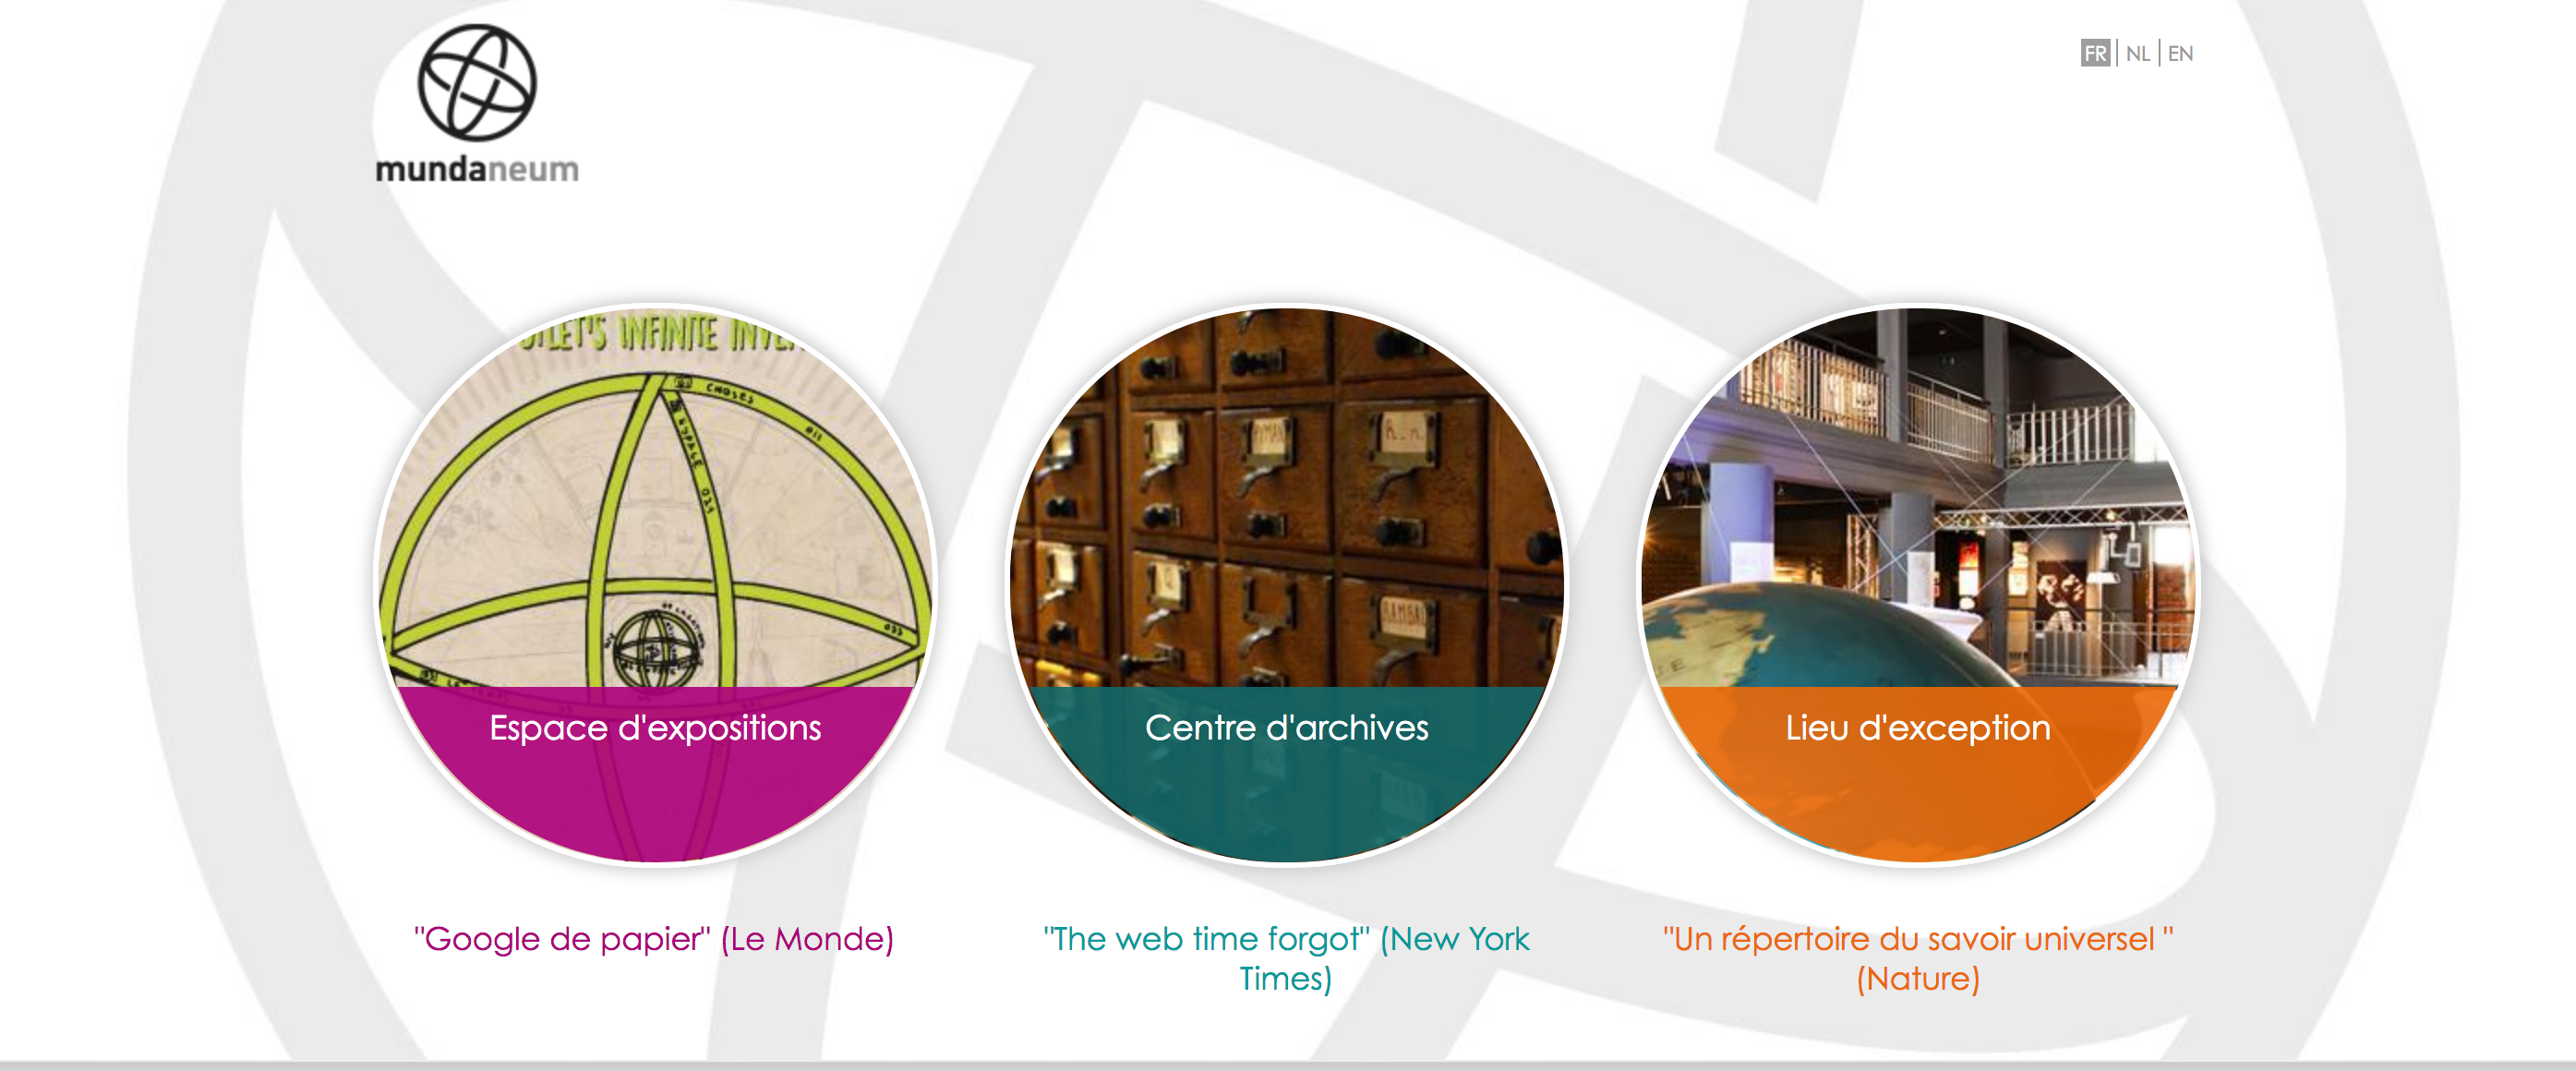
\includegraphics[scale=0.3]{mundaneum}
\caption{Capture-d'écran du site internet du \textit{Mundaneum}.}
\end{figure}

Diverses bibliothèques procèdent parallèlement au \textit{microfilmage} ou numérisation de leurs collections. En 1927, la Librairie du Congrès (États-Unis) procède au microfilmage de quelques trois millions de pages de livres et manuscrits de la \textit{British Library} (Angleterre). Les microfilms générés durant cette grande période de réhabilitation des documents sont encore utilisés aujourd'hui\footnote{\cite[p. 9]{thylstrup_politics_2018}}.

Vannevar Bush\footnote{Vannevar Bush (1890-1974), ingénieur et inventeur américain} décrit son invention le \textit{Memex}, convaincu que les méthodes traditionnelles d'indexation ne suffisent pas à répondre aux besoins des scientifiques modernes\footnote{\cite[p. 11]{xie_discover_2016}}, dans un fameux article publié en 1945, \og \textit{As We May Think} \fg{}. Il définit sans le savoir ce qui constituera nos futurs ordinateurs personnels.

\begin{quotation}
[\textit{Traduction}]
Il s'agit d'un appareil dans lequel un individu peut stocker tous ses livres, fichiers et communications. Cet appareil est mécanisé de façon à pouvoir être consulté avec flexibilité et rapidité. Il est semblable à un élargissement, dans un format réduit, de la mémoire de l'individu.
 \footnote{\inquote{\textit{[It is] a device in which an individual stores all his books, records, and communications, and which is mechanized so that it may be consulted with exceeding speed and flexibility. It is an enlarged intimate supplement to his memory}}\cite[p. 6]{weiss_using_2014}.}
 \end{quotation}

L'américain Richard Feynman\footnote{Richard Feynman (1918-1988), physicien et théoricien américain, précurseur en nanotechnologies.} conçoit dès 1959 les perspectives offertes par les nouvelles technologies et leurs potentiels impacts sur les pratiques des bibliothécaires et autres spécialistes de l'information. Sa conférence \emph{There's plenty of room at the bottom} donnée le 29 décembre 1959, lors de la réunion annuelle de l'\textit{American Physical Society (California Institute of Technology)} propose de comprimer l'intégralité de l'encyclopédie britannique afin de la réduire à la taille d'une tête d'épingle. Il ira même plus loin en concluant ses propos par la proposition de réduire l'intégralité de la connaissance humaine suivant la même méthode. Il imagine pour cela un système de conversion des caractères textuels en traits et points. Nous sommes un an avant le début des travaux sur l'\gls{ascii}\footnote{Norme étasunienne qui sert comme premier système d'encodage informatique des caractères en anglais et apportera un premier niveau de standardisation. Les caractères utilisés en anglais sont encodés suivant une combinaison de 0 et de 1.}\footnote{\cite[p. 25]{association_pour_le_patrimoine_naturel_et_culturel_du_canton_de_vaud_patrimoine_2012}}.

Dans son ouvrage \emph{Libraries of the Future}, paru en 1965,  J.C.R. Licklider\footnote{Joseph Carl Robnett Licklider (1915-1990), psychologue et informaticien américain.} propose d'étendre le monde des bibliothèques à celui des ordinateurs. Au-delà de l'objet livre, présenter faits et idées en fonctions, classes d'informations et domaines de connaissances, \inquote{\textit{[engineers] need to substitute for the book a device that will make it easy to transmit information without transporting material, and that will not only present information to people but also process it for them\footnote{\cite[p. 6]{weiss_using_2014}}.}} Il faudra encore plus d'une génération pour que le numérique soit pleinement appliqué à la gestion des livres et du contenu informationnel qu'ils contiennent.

Nous concluons cette section par le projet Gutenberg, lancé par Michel Hart\footnote{Michael Stern Hart (1947-2011), auteur américain et inventeur du livre électronique ou \textit{e-book.}} en 1971. Convaincu que la valeur ajoutée des ordinateurs ne se trouve pas uniquement dans leur puissance de calcul, mais également dans leur capacité à stocker et à retrouver des informations, il parvient à rassembler une équipe de volontaires pour saisir au clavier des textes libres de droit dans un format accessible et compréhensible par les ordinateurs : une version basique de l'\gls{ascii}. Ces textes analogues ainsi convertis dans une forme numérique sont conservés sur un serveur en mode texte, et diffusés auprès des membres du réseau \textit{ARPAnet\footnote{\textit{Advanced Research Projects Agency Network}, réseau qui a servi de modèle à notre actuel internet.}}\footnote{\cite[p. 10]{association_pour_le_patrimoine_naturel_et_culturel_du_canton_de_vaud_patrimoine_2012}}. L'objectif n'est alors pas la précision, mais une plus ou moins haute correspondance entre texte écrit et rendu numérique\footnote{\cite[p. 10]{thylstrup_politics_2018}}. Ce projet peut être perçu comme le premier projet de bibliothèque numérique, alors que l'internet et le web que nous connaissons aujourd'hui ne seront mis en place que dans les années 90.

\newpage
\begin{figure}[H]% force à placer l'image au sein de notre balise figure
\centering
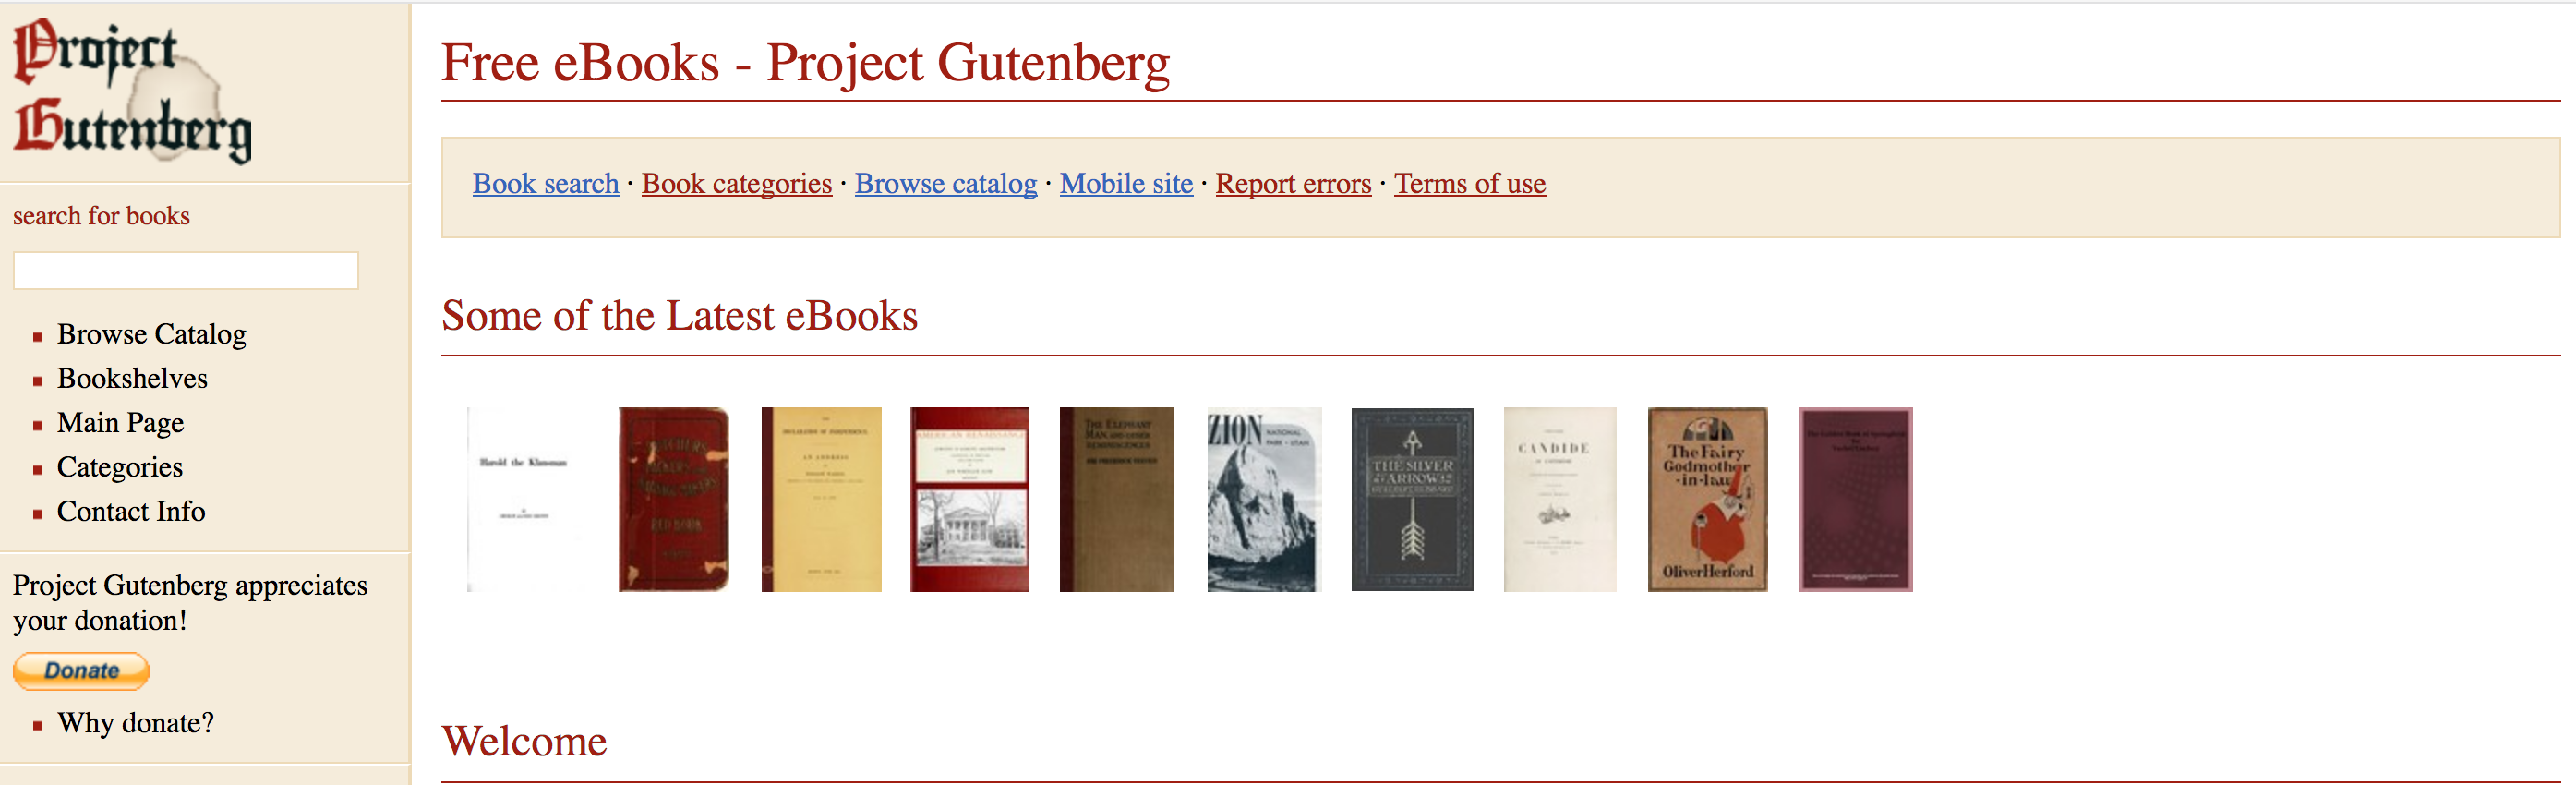
\includegraphics[scale=0.33]{projet_gutenberg}
\caption{Capture-d'écran du site internet du \textit{Projet Gutenberg}.}
\end{figure}

Les principaux défis techniques permettant le passage d'un texte physique à une version numérique sont levés entre 1970 et 1990 (le coût des scanners devient abordable pour les bibliothèques, les formats des images digitales se normalisent, l'industrie des logiciels s'intéresse aux programmes de \gls{reo})\footnote{\cite{association_pour_le_patrimoine_naturel_et_culturel_du_canton_de_vaud_patrimoine_2012}}. 

Désormais les écrans et les claviers servent d'interface entre hommes et ordinateurs, la puissance informatique a été augmentée et les premiers systèmes de recherche documentaires voient le jour\footnote{\cite[p. 10]{weiss_using_2014}}. Pour plus de détails sur ces développements du matériel informatique, liés à l'avènement d'internet\footnote{L'ensemble des supports de cours élaborés par Mr. Philippe Bootz, dans le cadre du cours "Sémiotique du numérique", suivis durant ma première année de Master en \textit{Humanités numériques : enjeux et technologies}, Université Paris 8, ont servis à l'élaboration de la synthèse des éléments techniques.}, référez-vous à l'annexe \ref{premisse}. 
\newpage

\begin{figure}[H]% force à placer l'image au sein de notre balise figure
%\centering
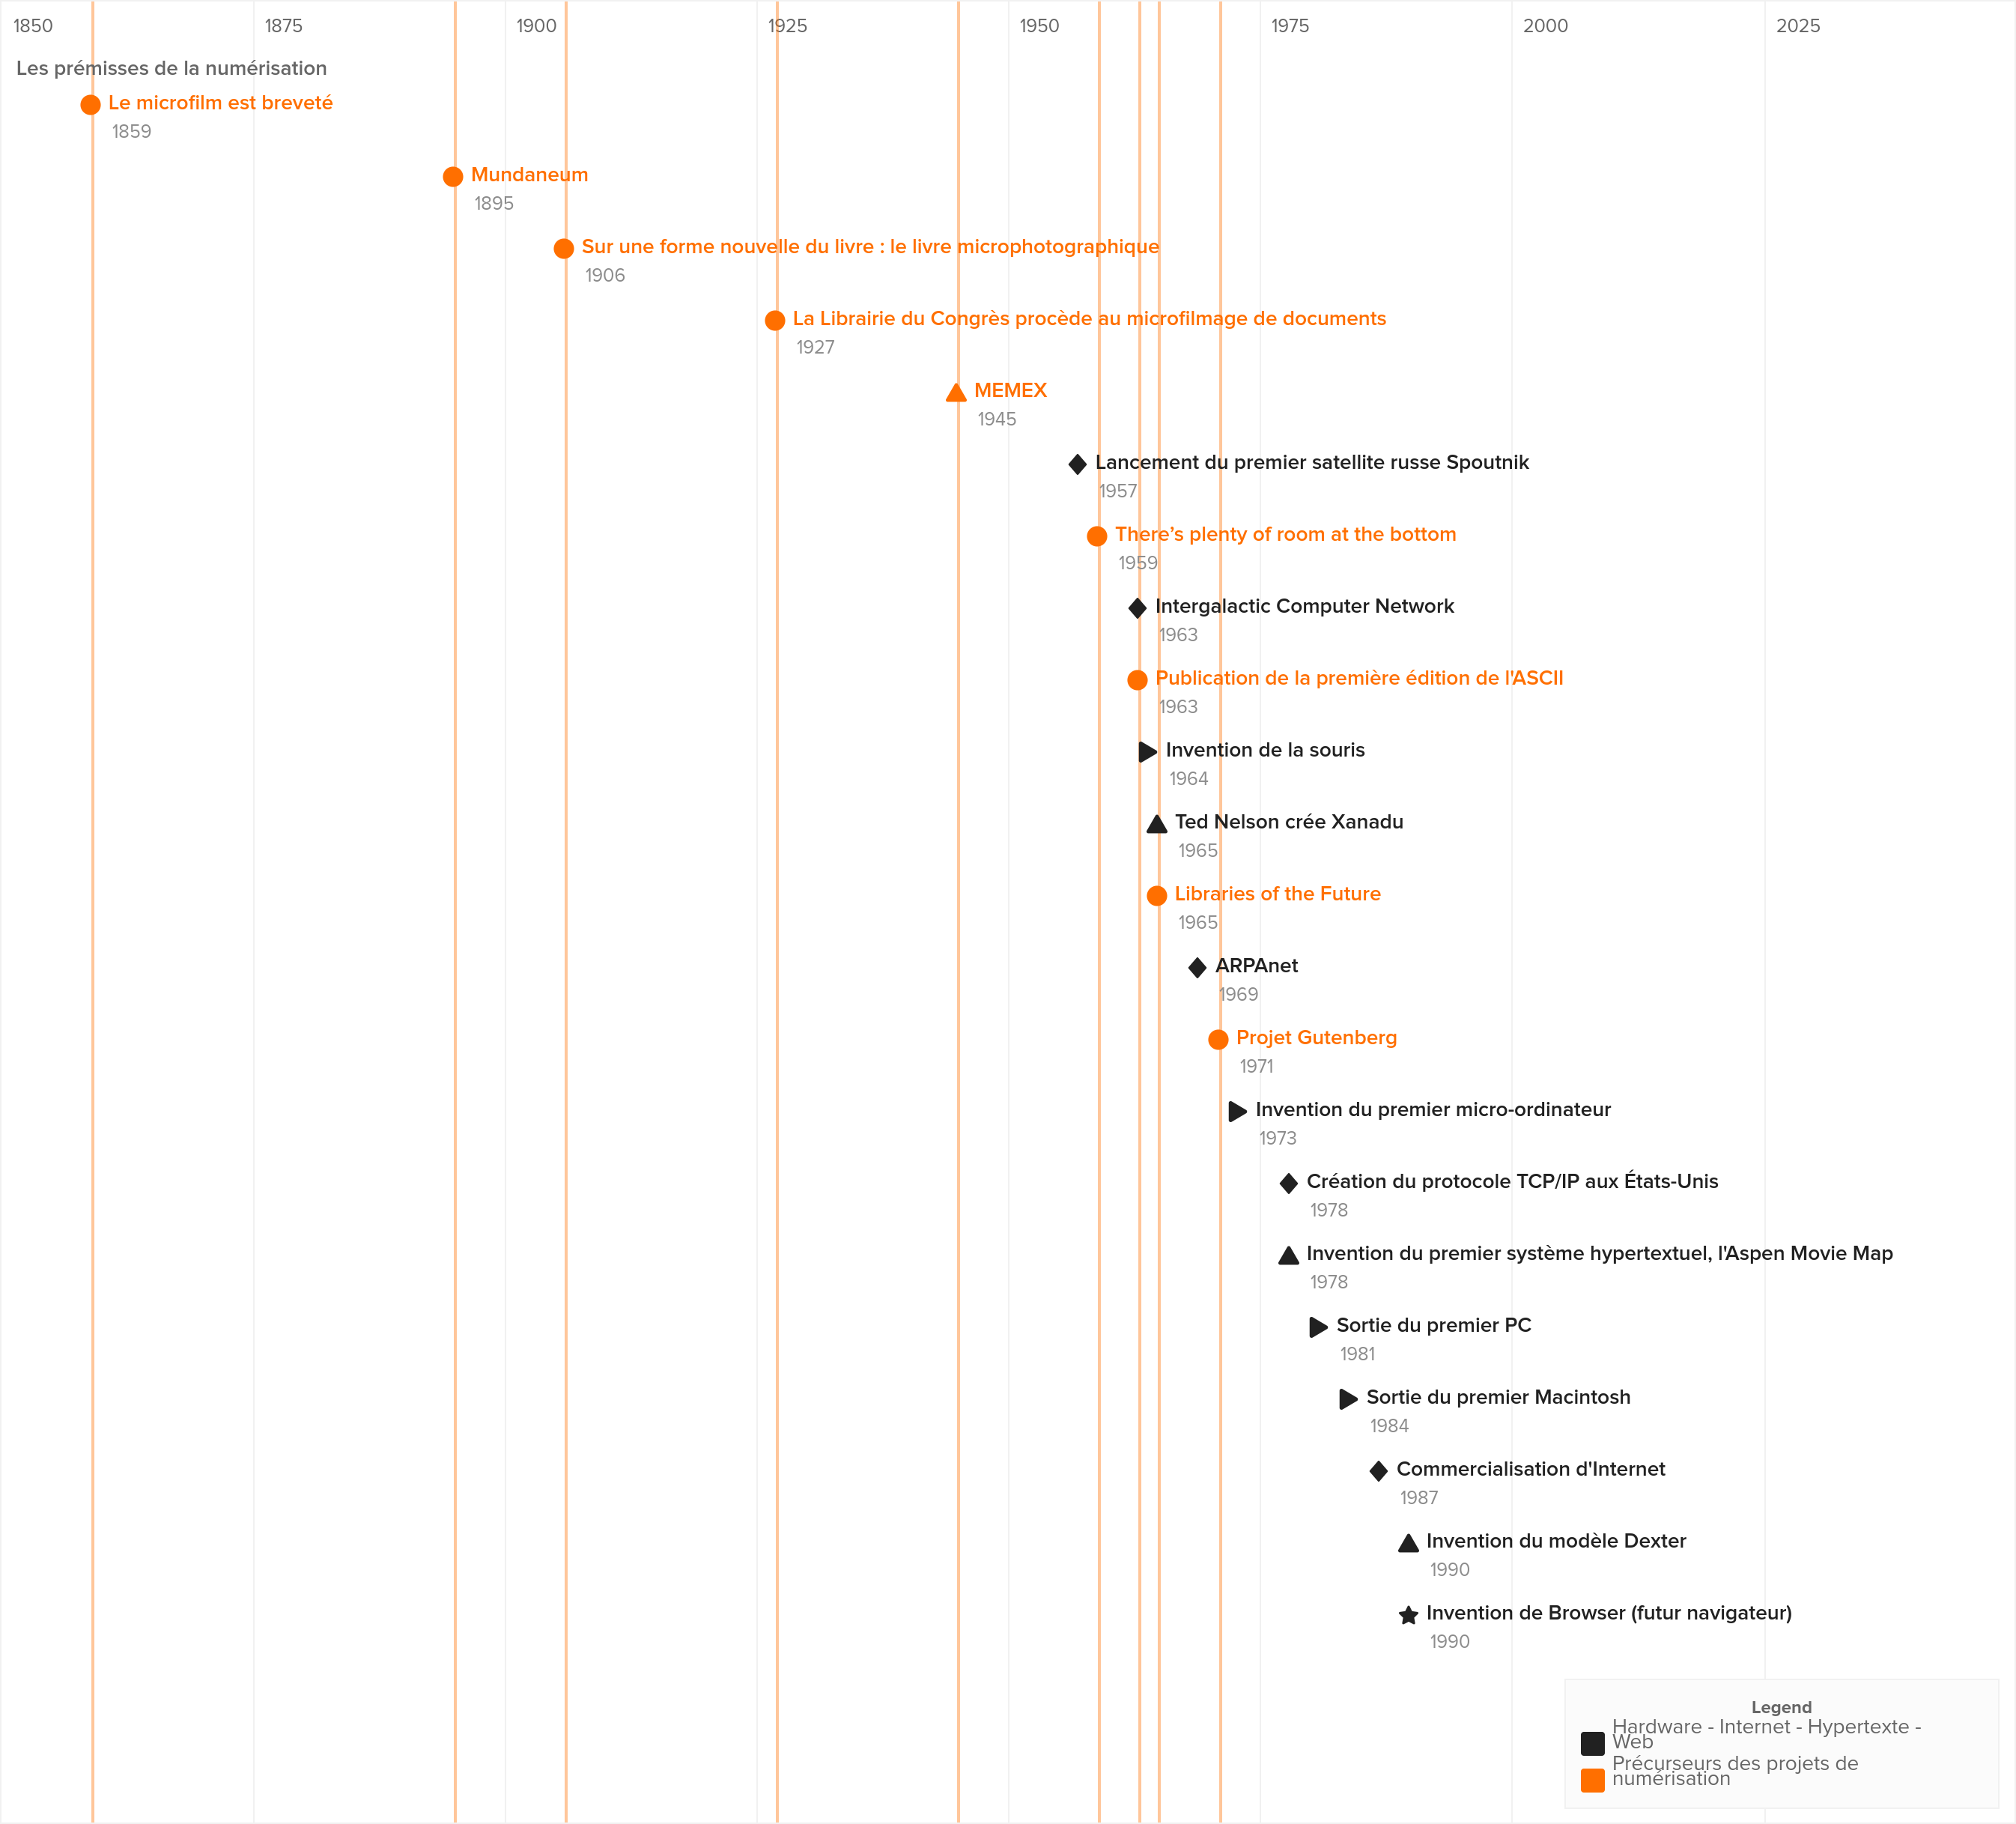
\includegraphics[angle=90, scale=0.21]{premisse_image.png}
\caption{Frise temporelle, \textit{Les prémisses de la numérisation}.}
\end{figure}
\newpage

%========PASSAGE A L'ECHELLE
\section{1990-2000 : Passage à l'échelle}\label{echelle}
%des bibliothèques numériques aux entreprises de numérisation de masse
Bien que les bibliothèques publiques apparaissent dès le milieu du 19\up{e} siècle\footnote{\cite[p.230]{jones_public_2017}}, avec pour vocation de rendre la connaissance accessible à tous, ce n'est qu'au début des années 1990 et l'avènement des ordinateurs personnels, que le mouvement des bibliothèques numériques voit le jour. Au-delà des développements purement techniques, les professionnels réalisent que proposer des collections numériques signifie bien plus que l'acte de \gls{num}, et que le processus est étroitement lié à des enjeux et des controverses culturelles, politiques et légales. Mais comment est-on passé de la bibliothèque numérique, aux projets de numérisation de masse ? 

Nous tenterons dans cette section de proposer une chronologie résumée des faits les plus marquants de cette révolution. Il est important de relever qu'il n'existe pas encore de définition exacte ni de catégorisation pour des projets d'une telle ampleur, et nous avons pu croiser, durant notre état de l'art, les expressions \textit{very large digital libraries} ou \textit{massive digital libraries\footnote{\cite{weiss_using_2014}}} au même titre que \textit{large-scale digitization projects\footnote{\cite[p.47]{lampert_ramping_2018}}\footnote{\cite{yeates_collaborative_2006}}} ou \textit{projets de numérisation de masse}\footnote{\cite{thylstrup_politics_2018}}\footnote{\cite{lampert_ramping_2018}}\footnote{\cite{xie_discover_2016}} pour désigner ces entreprises. Par souci de cohérence et puisque le cadre théorique fait encore débat, nous avons choisi de regrouper toutes les initiatives sous l'appellation de \textit{projets de numérisation de masse}.

Avec la démocratisation de l'ordinateur personnel et la naissance du web, les premières bibliothèques numériques voient le jour. Différents termes servent à les désigner, \textit{electronic library, virtual library, network-accessible libraries, libraries without walls}, reflétant l'évolution du sens de cette expression\footnote{\cite[p.3]{xie_discover_2016}}. D'abord perçues d'un point de vue technique et non comme institution ou objets porteurs d'influences sociales, \inquote{\textit{In this sense, they are an extension and enhancement of information storage and retrieval systems that manipulate digital data in any medium (text, image, sound ; static or dynamic images) and exist in distributed networks}\footnote{\cite[p.243]{jones_public_2017}}}, les bibliothèques numériques garderont trace de ce premier focus technologique\footnote{\cite[p.245]{jones_public_2017}}. 

Karen Calhoun les définit comme un système  de services et de gestion des collections numériques, basé sur une architecture centrée sur les données\footnote{\cite{calhoun_exploring_2014}}.

Prenant conscience des potentialités en termes de services aux utilisateurs, promis par les interfaces numériques, les bibliothèques se mettent à réfléchir au développement de leurs activités, laissant les informaticiens développer les systèmes requis\footnote{\cite{jones_public_2017}}. Les premières entreprises de numérisation sont pensées dans la complémentarité de la mission d'accessibilité de la connaissance humaine, et motivées par les perspectives de préservation de documents rares ou trop fragiles, le rayonnement supplémentaire apporté aux collections et aux institutions par cet accès en ligne, et la possibilité de numériser différents matériaux (photographies, textes, manuscrits etc.)\footnote{\cite[p.274]{lopatin_library_2006}}. Les projets de numérisation héritent toutefois des mêmes biais que les premières collections des bibliothèques publiques, dont les politiques documentaires visaient à élever l'esprit des masses\footnote{\cite{jones_public_2017}}. 

\begin{quotation}
[\textit{Traduction}]
Les programmes de numérisation des bibliothèques ont contribué à la création d'un répertoire de collections spécialisées et de services dédiés à une audience similaire à celle de la bibliothèque physique. Puisque la plupart des bibliothèques engagées dans ces programmes de numérisation sont académiques, les collections sont destinées à un usage d'abord scientifique.\footnote{\inquote{\textit{[...] library digitization programs have largely aimed to establish a repertoire of fairly specialized collections and services targeted at an audience that resembles the host libraries patron base - which, since most digitizing libraries are academics libraries, means designing for scholarly use}}\cite[p.247]{jones_public_2017}.}
\end{quotation}

\begin{quotation}
[\textit{Traduction}]
Les bibliothèques numériques et les bibliothèques publiques se sont aliénées de potentiels utilisateurs en se focalisant trop sur leurs idéaux. Les bibliothèques publiques en traitant de haut les travailleurs et ouvriers, les faisant se sentir indésirables et les bibliothèques numériques en développant des interfaces demandant une connaissance technique, culturelle ou thématique préalable à leur utilisation.
\footnote{\inquote{\textit{[...] both have alienated potential users by holding too strictly to this ideal, public libraries by making factory workers and other laborers feel patronized and unwelcome, and digital libraries by presenting interfaces that require a particular sort of technological, cultural, or domain-specific knowledge in order to use them effectively}}\cite[p.247]{jones_public_2017}.}
\end{quotation}

\textit{The Perseus Digital Library}, est l'un des premiers projets de bibliothèque numérique. Initié en 1985 au sein de l'université Tufts (États-Unis), la version initiale regroupe des textes grecs et leurs traductions anglaises sur un CD-ROM. Le projet évolue vers une première plateforme en ligne en 1995, ouvrant ses collections au monde greco-romain et passant d'un outil d'enseignement à un moteur de recherche. Il rassemble des ressources liées aux études classiques (civilisations grecques et romaines) jusqu'à la renaissance anglaise\footnote{\cite{dubis_web_2003}}.

\begin{figure}[H]% force à placer l'image au sein de notre balise figure
\centering
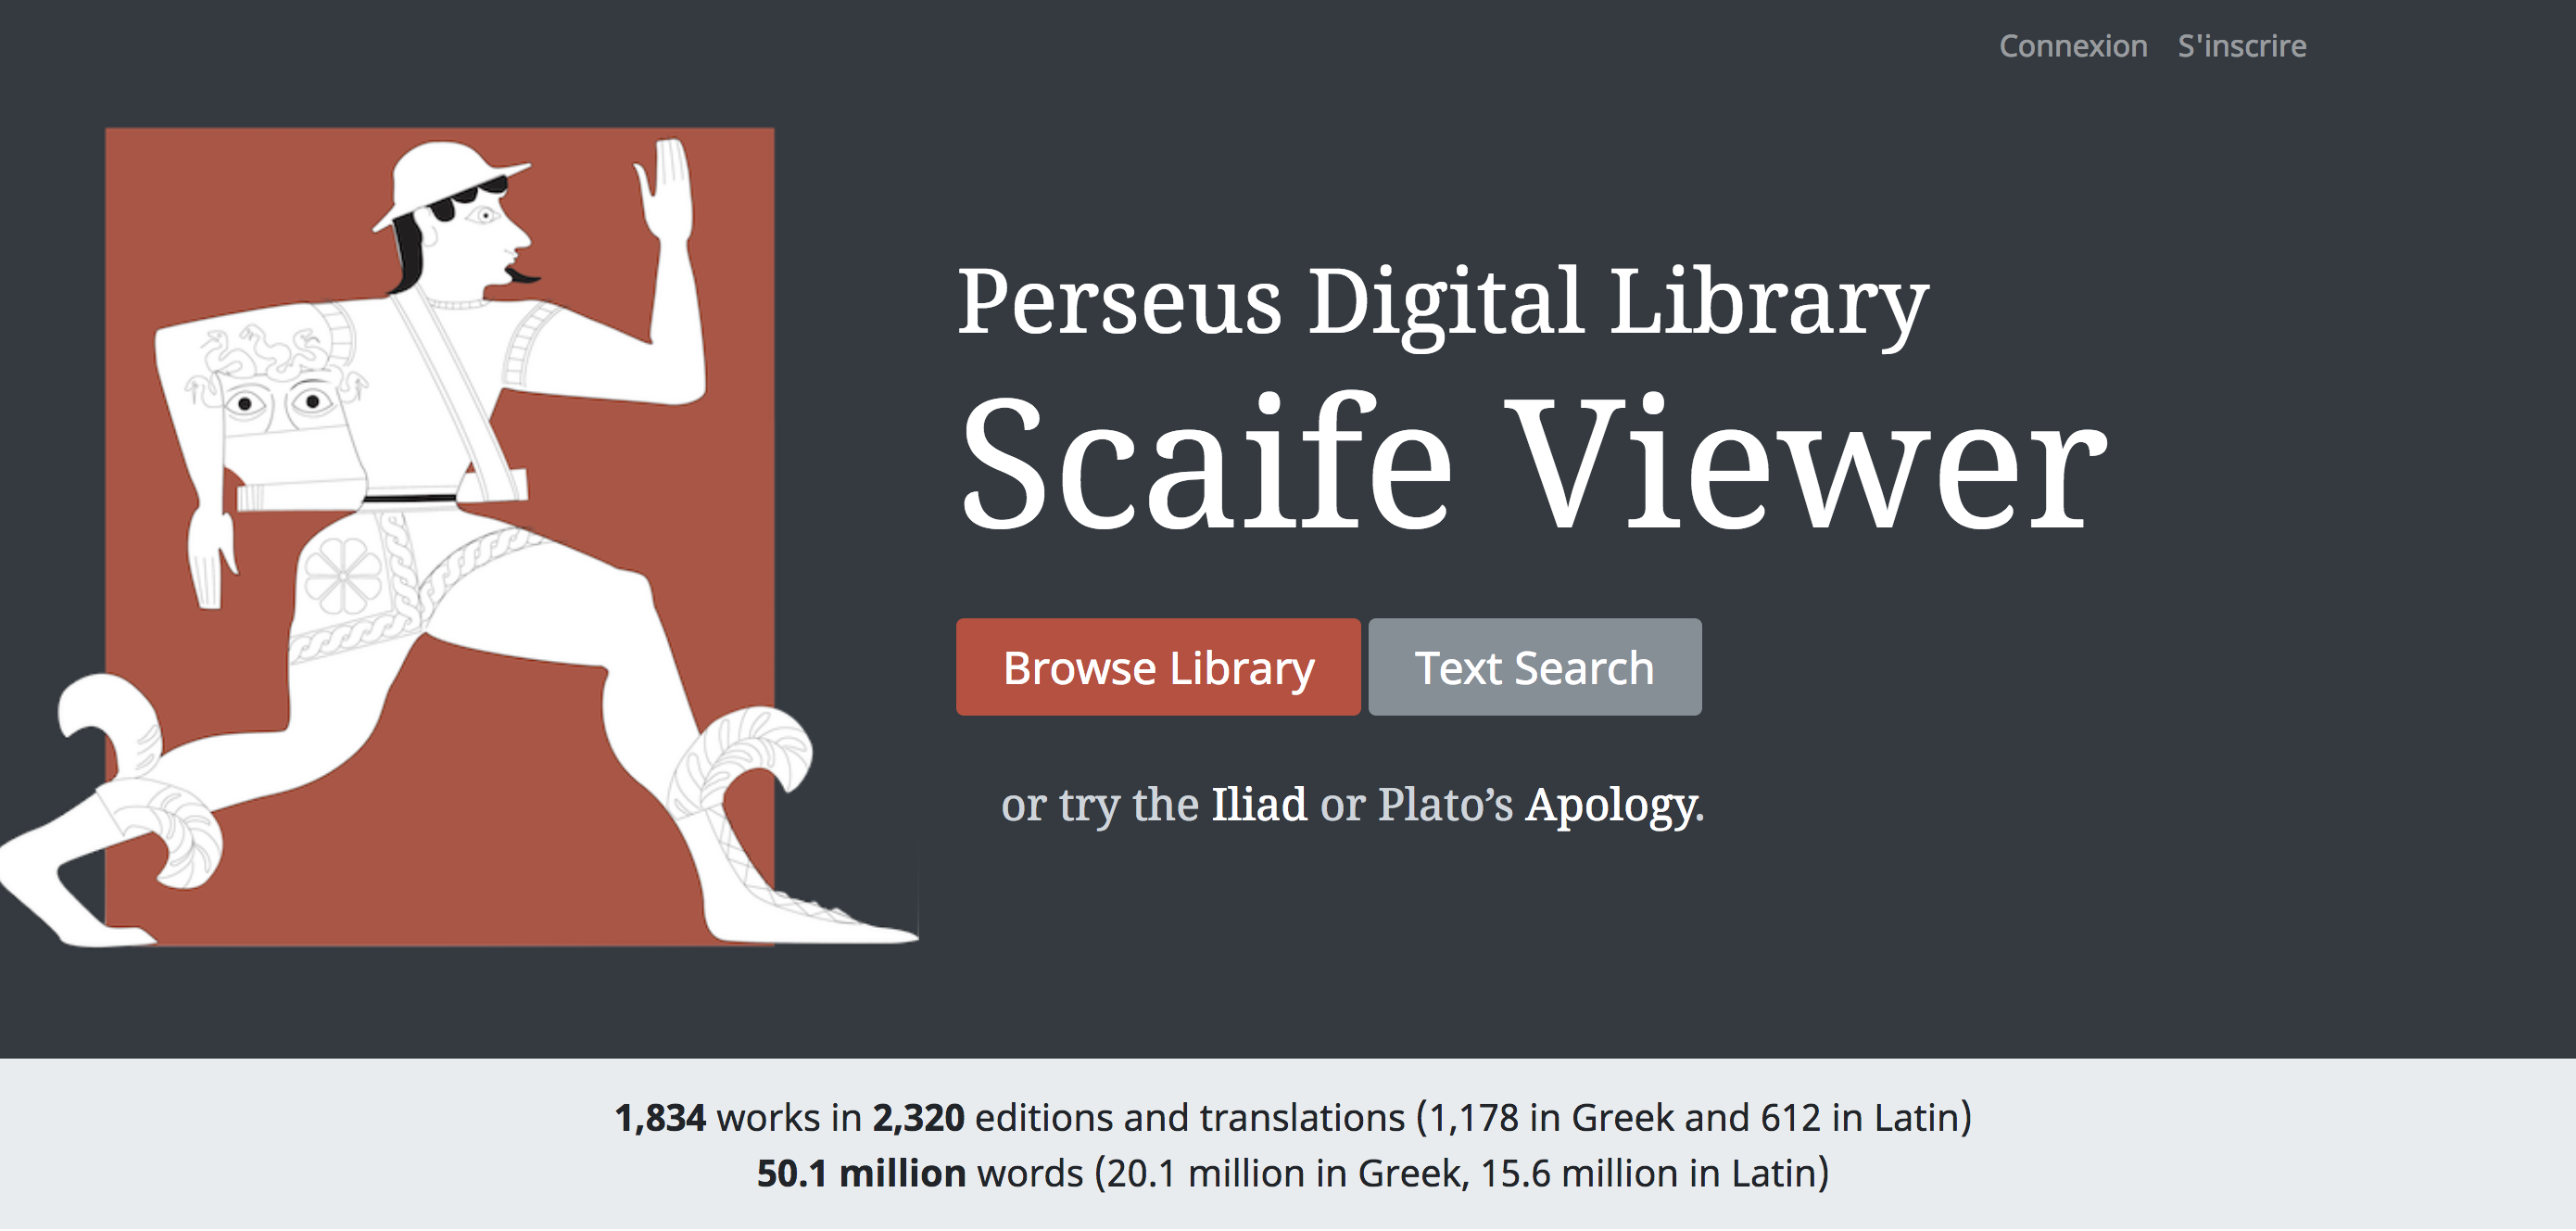
\includegraphics[width=15cm]{perseus}
\caption{Capture-d'écran du visualisateur \textit{Scaife} de la \textit{Perseus Digital Library}.}
\end{figure}

Si ces premières initiatives de numérisation sont ciblées sur une certaine catégorie de collection et vers une audience particulière, c'est pour des raisons de financement. Les institutions culturelles et patrimoniales y voient  une opportunité pour augmenter l'accessibilité de leurs collections et bénéficient dès les premiers temps de fonds publics\footnote{\cite[p.1]{coutts_stepping_2017}}. Les entreprises de numérisation articulent différents champs, nécessitant la création de nouveaux standards et bonnes pratiques, qui mèneront à l'élargissement de la portée de ces projets. 

\begin{quotation}
[\textit{Traduction}]
Il est apparu clairement que c'était un domaine multi-facettes, demandant une uniformisation des processus liés au contenu, aux technologies, à l'infrastructure, à la propriété intellectuelle et à la préservation. Les \gls{glam} ont très vite fait partie des participants les plus enthousiastes. En terme de contenu, les projets à petites échelles sont emblématiques des premières entreprises, se focalisant souvent sur ceux à haute valeur intellectuelle et culturelle. Cependant les activités de cette période visaient en parallèle à la mise en place de standards technologiques, au développement des infrastructures et au déploiement des processus de gestions, de préservation et de respect du droit d'auteur.
\footnote{\inquote{\textit{It also became clear that it was a multifaceted field, requiring that same process to be applied to issues of content, technology, infrastructure, intellectual property and sustainability. Universities, museums, galleries and national libraries were amongst the enthusiastic participants. In term of contents, small-scale projects typified the early work, often showcasing items of major intellectual and cultural value. The activity in this period, however, was as much concentrated on developing experience in and standards for the use of the technology and the provision of infrastructure, legal management and preservation}}\cite[p.12]{coutts_stepping_2017}.}
\end{quotation}

Les premières initiatives de numérisation de masse semblent également issues d'une forme de croyance répandue chez les informaticiens, déclarant que l'information contenue sur le papier deviendrait un jour obsolète, \inquote{\textit{[...] there was an attitude in computer science that putting things on dead trees was obsolete and getting it all into a searchable, digital format was a quest that had to be accomplished someday}\footnote{\cite{cook_googles_nodate}}.} En proposant des livres sous forme numérique, ces pionniers argumentent également qu'ils mettent leurs informations à disposition de tous, utilisant le même motif que pour la création des bibliothèques publiques et reproduisant à nouveau leurs biais\footnote{\cite[p.8]{thylstrup_politics_2018}}.

\begin{quotation}
[\textit{Traduction}]
Tout comme au 19\up{e} siècle, il n'était pas suffisant de laisser le marché proposer des fictions de moindre qualité au peuple sans leur donner accès à des contenus jugés plus pertinents, au 21\up{e} siècle, il n'est pas suffisant de laisser les chercheurs errer sur internet face à un océan de sites, où le meilleur de la connaissance - naturellement contenu dans les livres - n'est pas accessible.
\footnote{\inquote{\textit{Just as in the nineteenth century, it was not seen as sufficient to let the market provide cheap paperback fiction for the masses without giving them access to higher quality materials, in the twenty-first century it is not enough to leave Internet searchers to their own devices in a sea of websites where the best knowledge - that contained in books - is nowhere to be found}}\cite[p.254]{jones_public_2017}.}
\end{quotation}

Le premier projet de numérisation massive répertorié en France est un véritable précurseur et apparaît au tout début des années 90, il découle de la création de la \gls{bnf} en 1989. À la demande du Président François Mitterand, Alain Giffard\footnote{Alain Giffard est directeur du groupement d’intérêt scientifique « Culture-médias \& numérique. » Il a été directeur informatique de la Bibliothèque de France, directeur adjoint de l’Institut Mémoires de l’édition contemporaine (Imec), conseiller technique de la ministre de la Culture et de la Communication pour la société de l’information et président de la mission interministérielle pour l’accès public à l’internet.} est prié d'utiliser les dernières innovations technologiques pour rendre accessible les ouvrages du catalogue de la \gls{bnf} et créer ainsi une très grande bibliothèque. Le projet conduira à la numérisation de 70'000 à 80'000 titres. Pour choisir quels ouvrages numériser, il n'eut pas recours à des bibliothécaires mais à des scientifiques et écrivains, ce qui fut possible car le projet était directement lié au Président. Alain Giffard explique d'ailleurs qu'il a personnellement acheté un grand nombre des livres à numériser, puisqu'ils n'étaient pas dans les collections de la \gls{bnf}, et que celle-ci avait du mal à collaborer avec ce projet. Cet exemple illustre bien le fait que les projets de numérisation massive, au-delà des enjeux techniques, sont aussi des questions politiques qui soulèvent des débats de territorialité (institutionnelle ou nationale), matérialité et culture\footnote{\cite[p.11]{thylstrup_politics_2018}}.  

Ces documents numérisés seront intégrés en 1997 au projet plus connu de numérisation massive, \textit{Gallica}. Ce projet, également mandaté par le Président François Mitterand, vise à numériser les livres libres de droit issus des collections de la \gls{bnf}, depuis le Moyen-Âge jusque vers 1930, avec une priorité pour les documents illustrant la culture francophone. Environ quatre millions de documents sont disponibles sur la plateforme du projet\footnote{\cite[p.140]{thylstrup_politics_2018}}.

\begin{figure}[H]% force à placer l'image au sein de notre balise figure
\centering
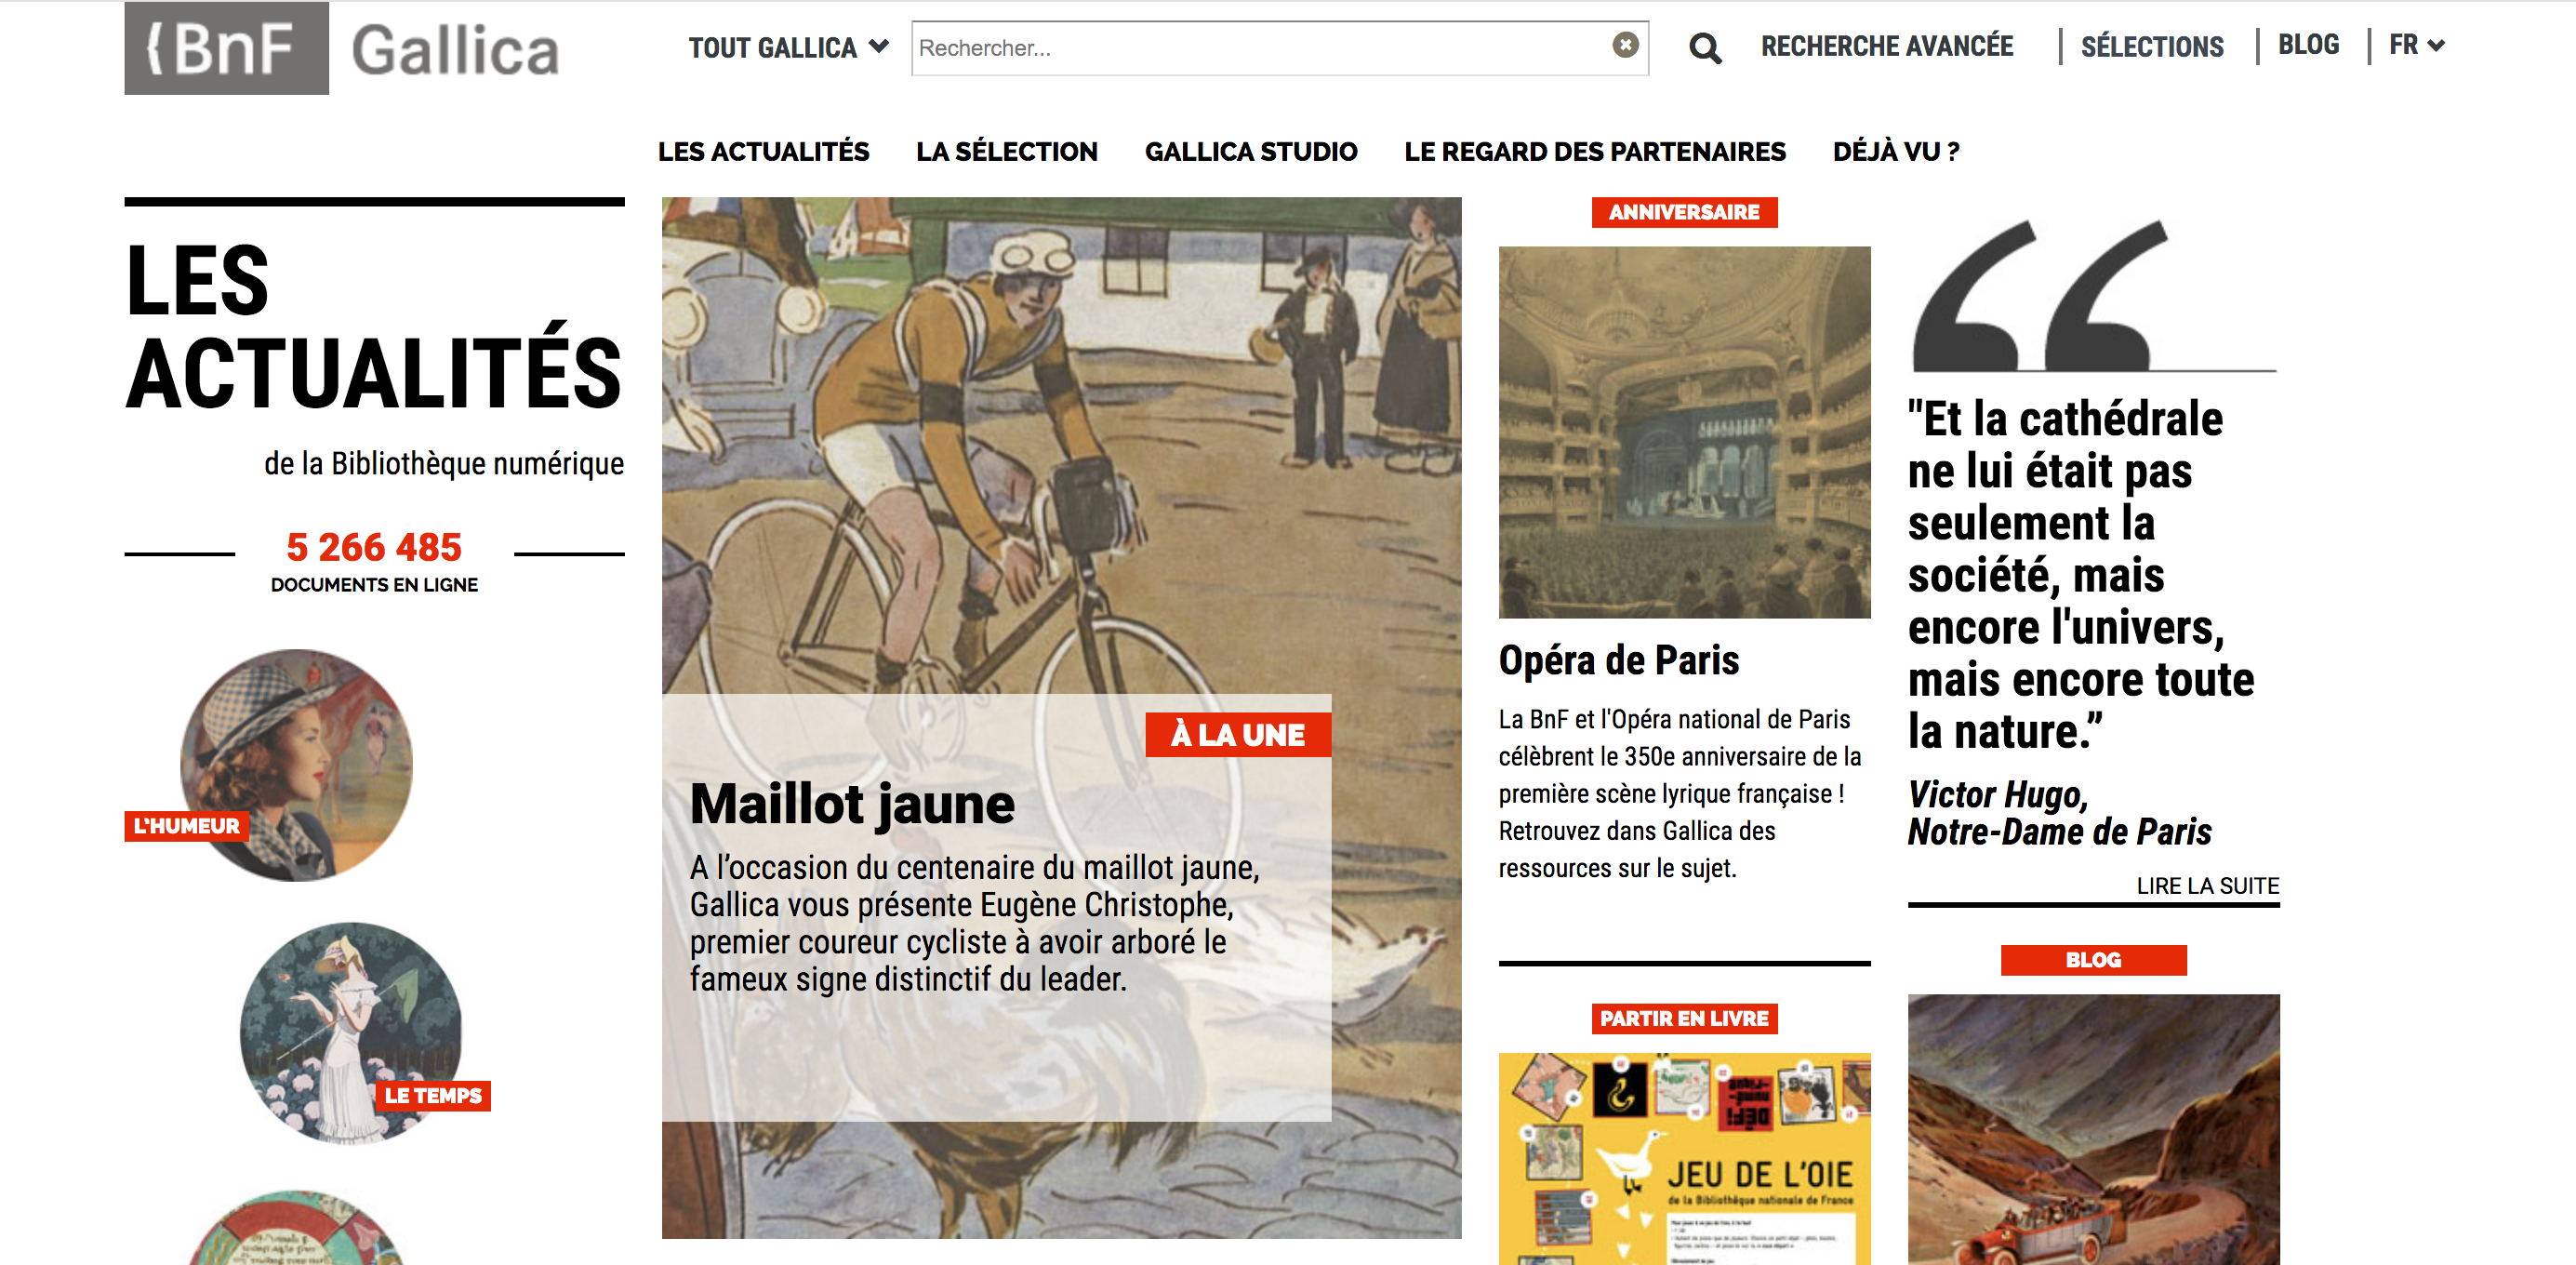
\includegraphics[width=15cm]{gallica}
\caption{Capture-d'écran de la plateforme du projet \textit{Gallica}.}
\end{figure}
L'\textit{Universal Digital Library} est initiée en 1995 par différents scientifiques en partenariat avec la Canergie Mellon Foundation (États-Unis). En 1998, ce projet est à l'origine du \textit{Thousand Book Project} qui sera finalement augmenté jusqu'à devenir le \textit{Million Book Project}, successivement terminé en 2007. Il se distingue des autres projets de numérisation de masse, en incluant dès le départ des institutions chinoises, indiennes ou égyptiennes. L'entreprise de numérisation s'est toutefois terminée en 2008\footnote{\cite[p.12]{thylstrup_politics_2018}}, et la plateforme du projet n'est pas parfaitement maintenue. Cet exemple, pourtant ambitieux, démontre que l'avenir réservé à de nombreux projets de numérisation est toujours bien incertain\footnote{\cite[p.12]{weiss_using_2014}}. Andrew Weiss appelle à une meilleure caractérisation des projets de numérisation de masse, afin d'en préserver l'accessibilité sur le long-terme et à sortir de tels projets des contraintes du marché économique : \inquote{\textit{However, in dealing with consortia of public and nonprofit educational institutions, market forces should not be the sole factor determining their overall sustainability, especially when the content is of significant cultural and social value\footnote{\cite[p.30]{weiss_using_2014}}.}}

\begin{figure}[H]% force à placer l'image au sein de notre balise figure
\centering
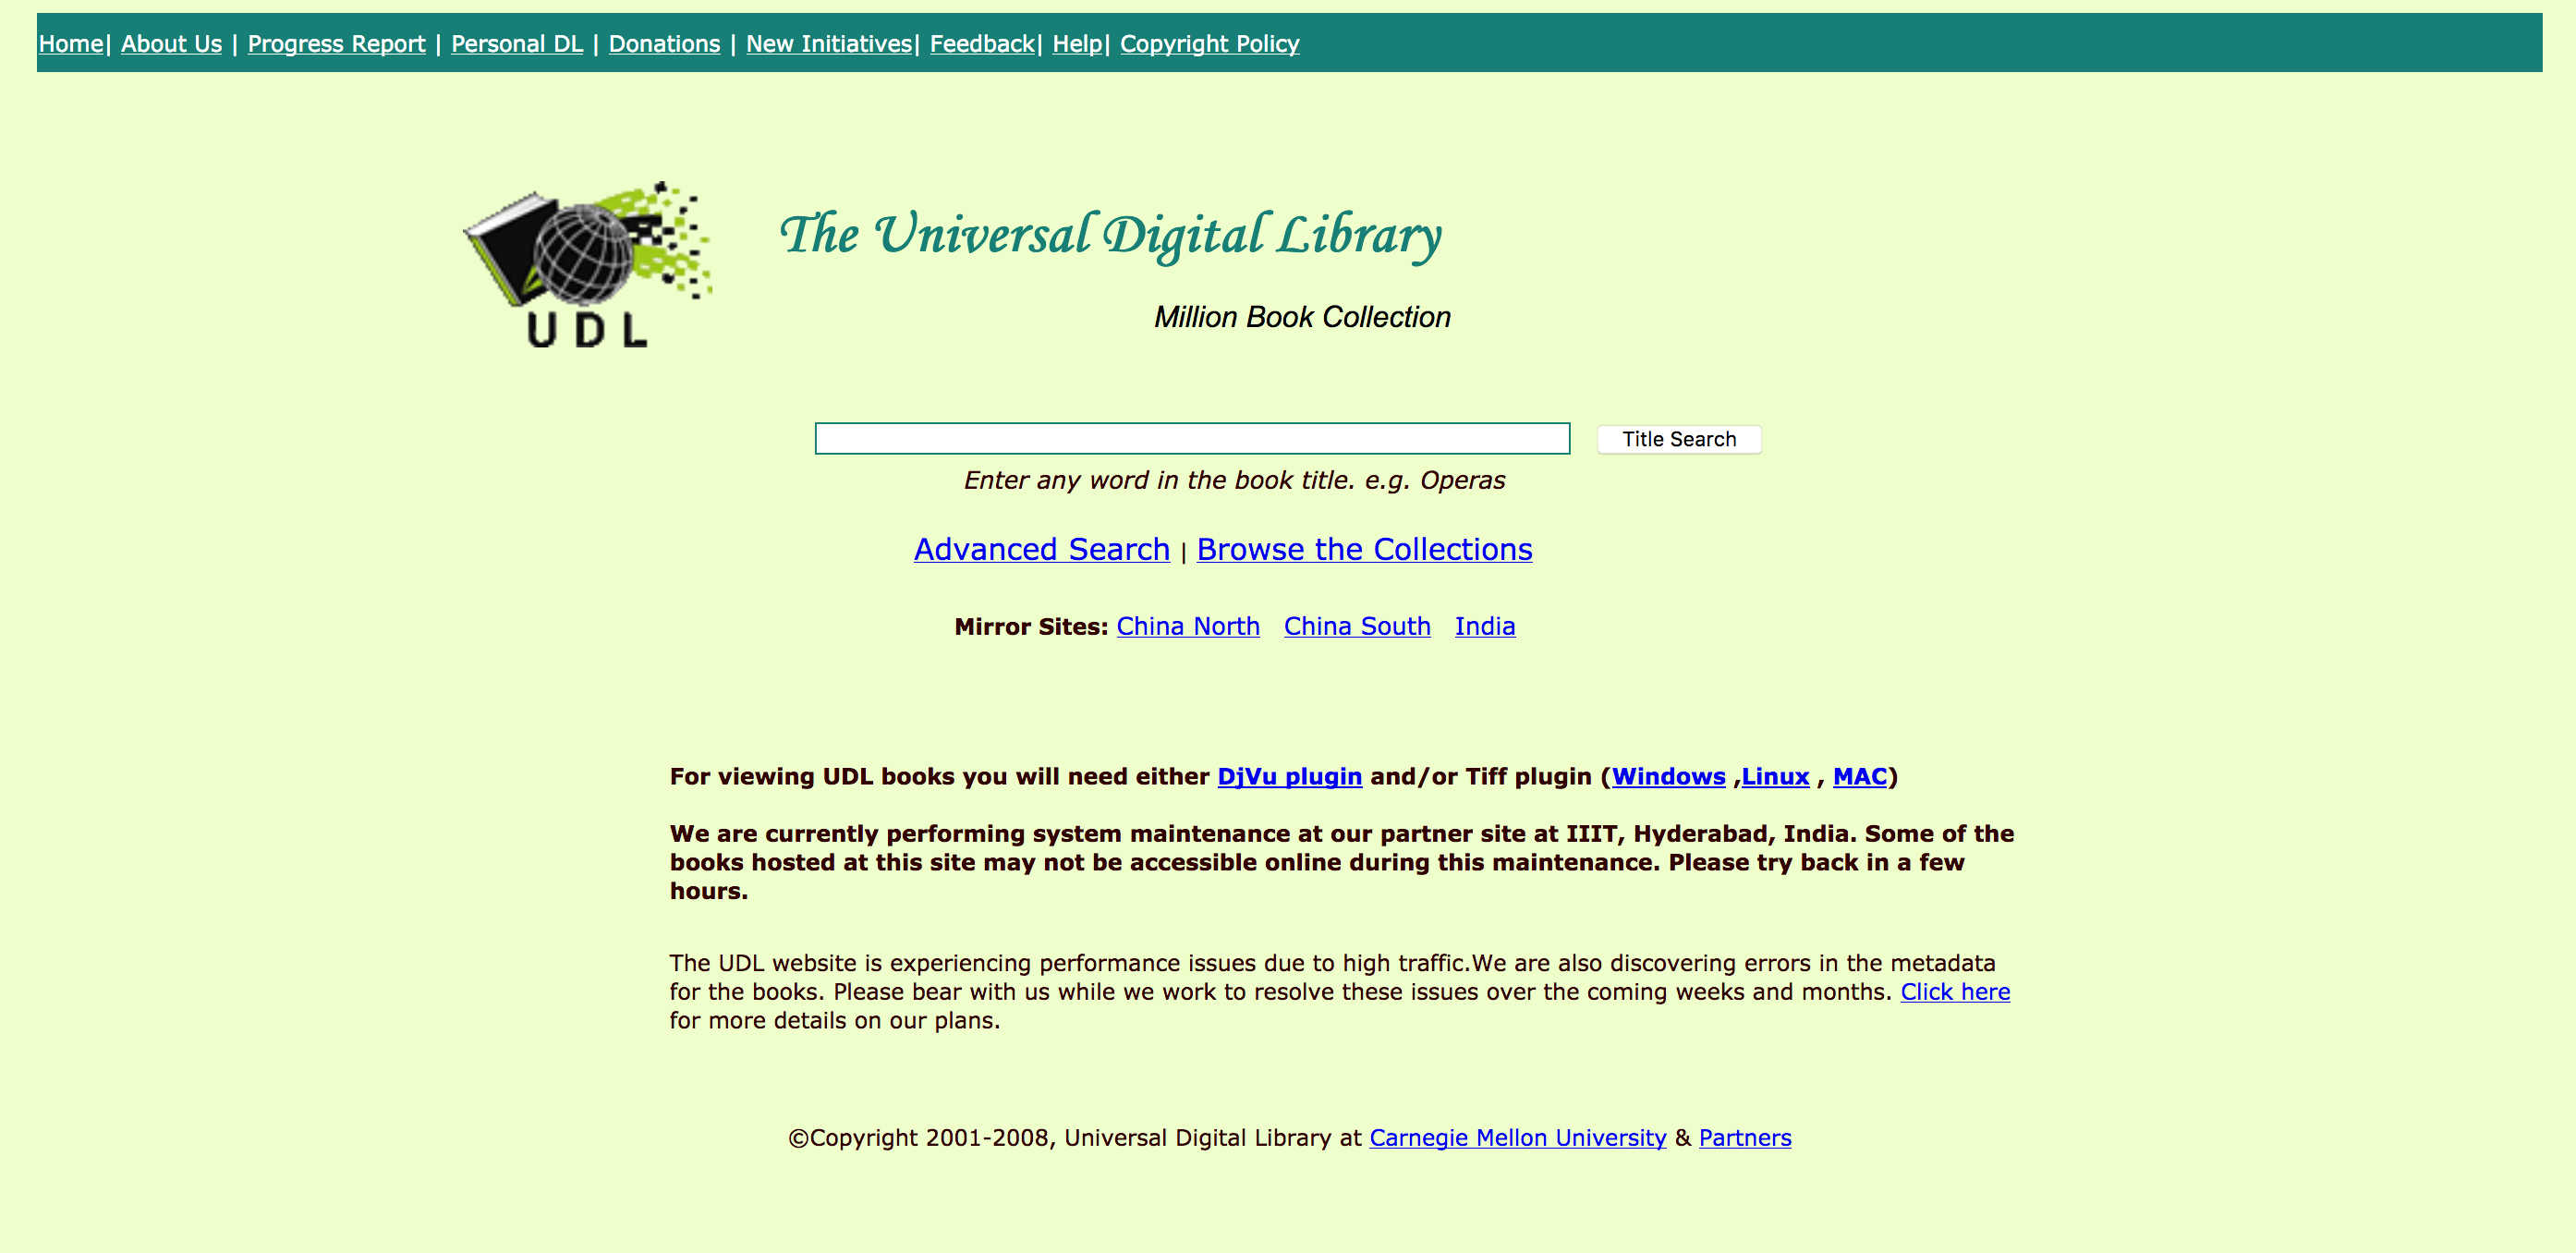
\includegraphics[width=15cm]{udl}
\caption{Capture-d'écran de la plateforme du projet \textit{Universal Digital Library}.}
\end{figure}

1996, marque également le lancement d'un projet se poursuivant aujourd'hui : \textit{The Internet Archive}. Fondé par l'activiste du \gls{oa} Brewster Kahle, avec pour objectif initial de préserver le matériel né numériquement (à l'instar des pages et des sites web). Le projet finira par numériser des livres dès 2005, avec l'aide d'une infrastructure regroupant de grandes institutions patrimoniales et acteurs privés, \textit{The Open Content Alliance}\footnote{\cite[p.12]{thylstrup_politics_2018}}.

Dans leur désir d'accessibilité, les projets de numérisation de masse ne tiennent d'abord pas compte des aspects légaux propres aux ouvrages numériques\footnote{\cite[p.251]{jones_public_2017}}, et se voient imposer un certain nombre de restrictions à ce désir d'ouverture. Toutefois l'ambition de construire une bibliothèque numérique universelle commence à se répandre, notamment au sein de l'entreprise Google\footnote{\cite{cook_googles_nodate}}. Il est important de spécifier qu'au début des années 2000 de nombreux standards et  bonnes pratiques ont été définis et ouvrent la voie aux futurs projets\footnote{\cite{dunning_digitising_2009}} : \inquote{\textit{The digital lifecycle is now well defined, moving from creation through curation, preservation, discovery and use to the creation of new knowledge and content\footnote{\cite[p.245]{jones_public_2017}}.}} Le mouvement des bibliothèques numériques va continuer de s'amplifier avec de nouveaux projets de numérisation de masse et l'apparition des dépôts de publication en \gls{oa}\footnote{\cite{xie_discover_2016}}\footnote{Comme notre mémoire porte sur les projets de numérisation de masse, nous n'aborderons la question du \gls{oa} qu'à travers certains développements du projet Time Machine.}. 

Les années 2000 marquent l'histoire des projets de numérisation par le séisme de \textit{Google Books} (2004) qui poussera les bibliothèques et leurs tutelles à revoir leurs stratégies de numérisation\footnote{\cite{dufrene_numerisation_2013}}, et sa réponse européenne \textit{Europeana} (2008). Le passage à l'échelle de ces initiatives est crucial dans l'industrialisation et la popularité du phénomène des \textit{\gls{bigd}}\footcite{thylstrup_politics_2018}\footnote{Nous ne parlerons pas en détail de l'histoire des big data dans le présent mémoire, mais pour l'anecdote, Time Machine n'est pas le premier projet à vouloir créer un big data du passé, le projet \textit{Collaborative for Historical Information and Analysis}, initié en 2011 par l'université de Pittsburgh poursuivait le même objectif. \cite{manning_big_2013}}.

Ces projets emblématiques des initiatives de numérisation de masse seront présentés en deuxième partie de ce mémoire, aux côtés d'autres initiatives similaires issues de ces dernières années.

L'apparition de projets de numérisation conduits par des entreprises à but lucratif semble marquer une séparation entre les initiatives issues du monde privé qui seraient par définition des \textit{massive digitisation projects} et celles du monde public des bibliothèques numériques, soit des \textit{massive digital libraries}\footnote{\cite[p.245]{jones_public_2017}}. Nous nous attacherons à déceler ces présupposées différences à travers l'analyse des réponses apportées par ces projets aux enjeux de la numérisation, qui sont souvent bien plus complexes.

%========POLITIQUE ET NUMERISATION EN EUROPE
\section{Politiques et numérisation}\label{politique}

L'histoire de la numérisation constitue également une histoire politique. L'\gls{ue} et \gls{unesco} témoignent toutes deux d'une certaine ambition.

En 2003, l'\gls{unesco} adopte la \textit{Charte sur le patrimoine numérique}, argumentant que le temps des solutions individuelles est révolu et que des solutions internationales doivent être mises en place pour faire face à la croissance des coûts liés à ces collections numérisées. L'article 11 appelle à une coopération de tous les acteurs :
\begin{quotation}
Vu la fracture numérique actuelle, il est nécessaire de renforcer la coopération et la solidarité internationales pour permettre à tous les pays d'assurer la création, la diffusion et la conservation de leur patrimoine numérique ainsi que la possibilité d'y accéder en permanence.
\end{quotation}
En 2009, le constat dressé par l'\gls{unesco} est amer, les recommandations non appliquées mettent l'humanité face au risque de perdre des pans entiers de son histoire\footnote{\cite{association_pour_le_patrimoine_naturel_et_culturel_du_canton_de_vaud_patrimoine_2012}}.

2009 est également l'année du lancement de la plateforme de la Bibliothèque numérique mondiale lancée par la Bibliothèque du Congrès sous l'égide de l'\gls{unesco} et visant à proposer une interface à large échelle aux collections patrimoniales numériques. Se sachant incapable de rivaliser avec d'autres grandes bibliothèques numériques, elle fait du multilinguisme et du choix sélectif des documents, ses principaux atouts\footnote{\cite{dufrene_numerisation_2013}}. 

\begin{figure}[H]% force à placer l'image au sein de notre balise figure
\centering
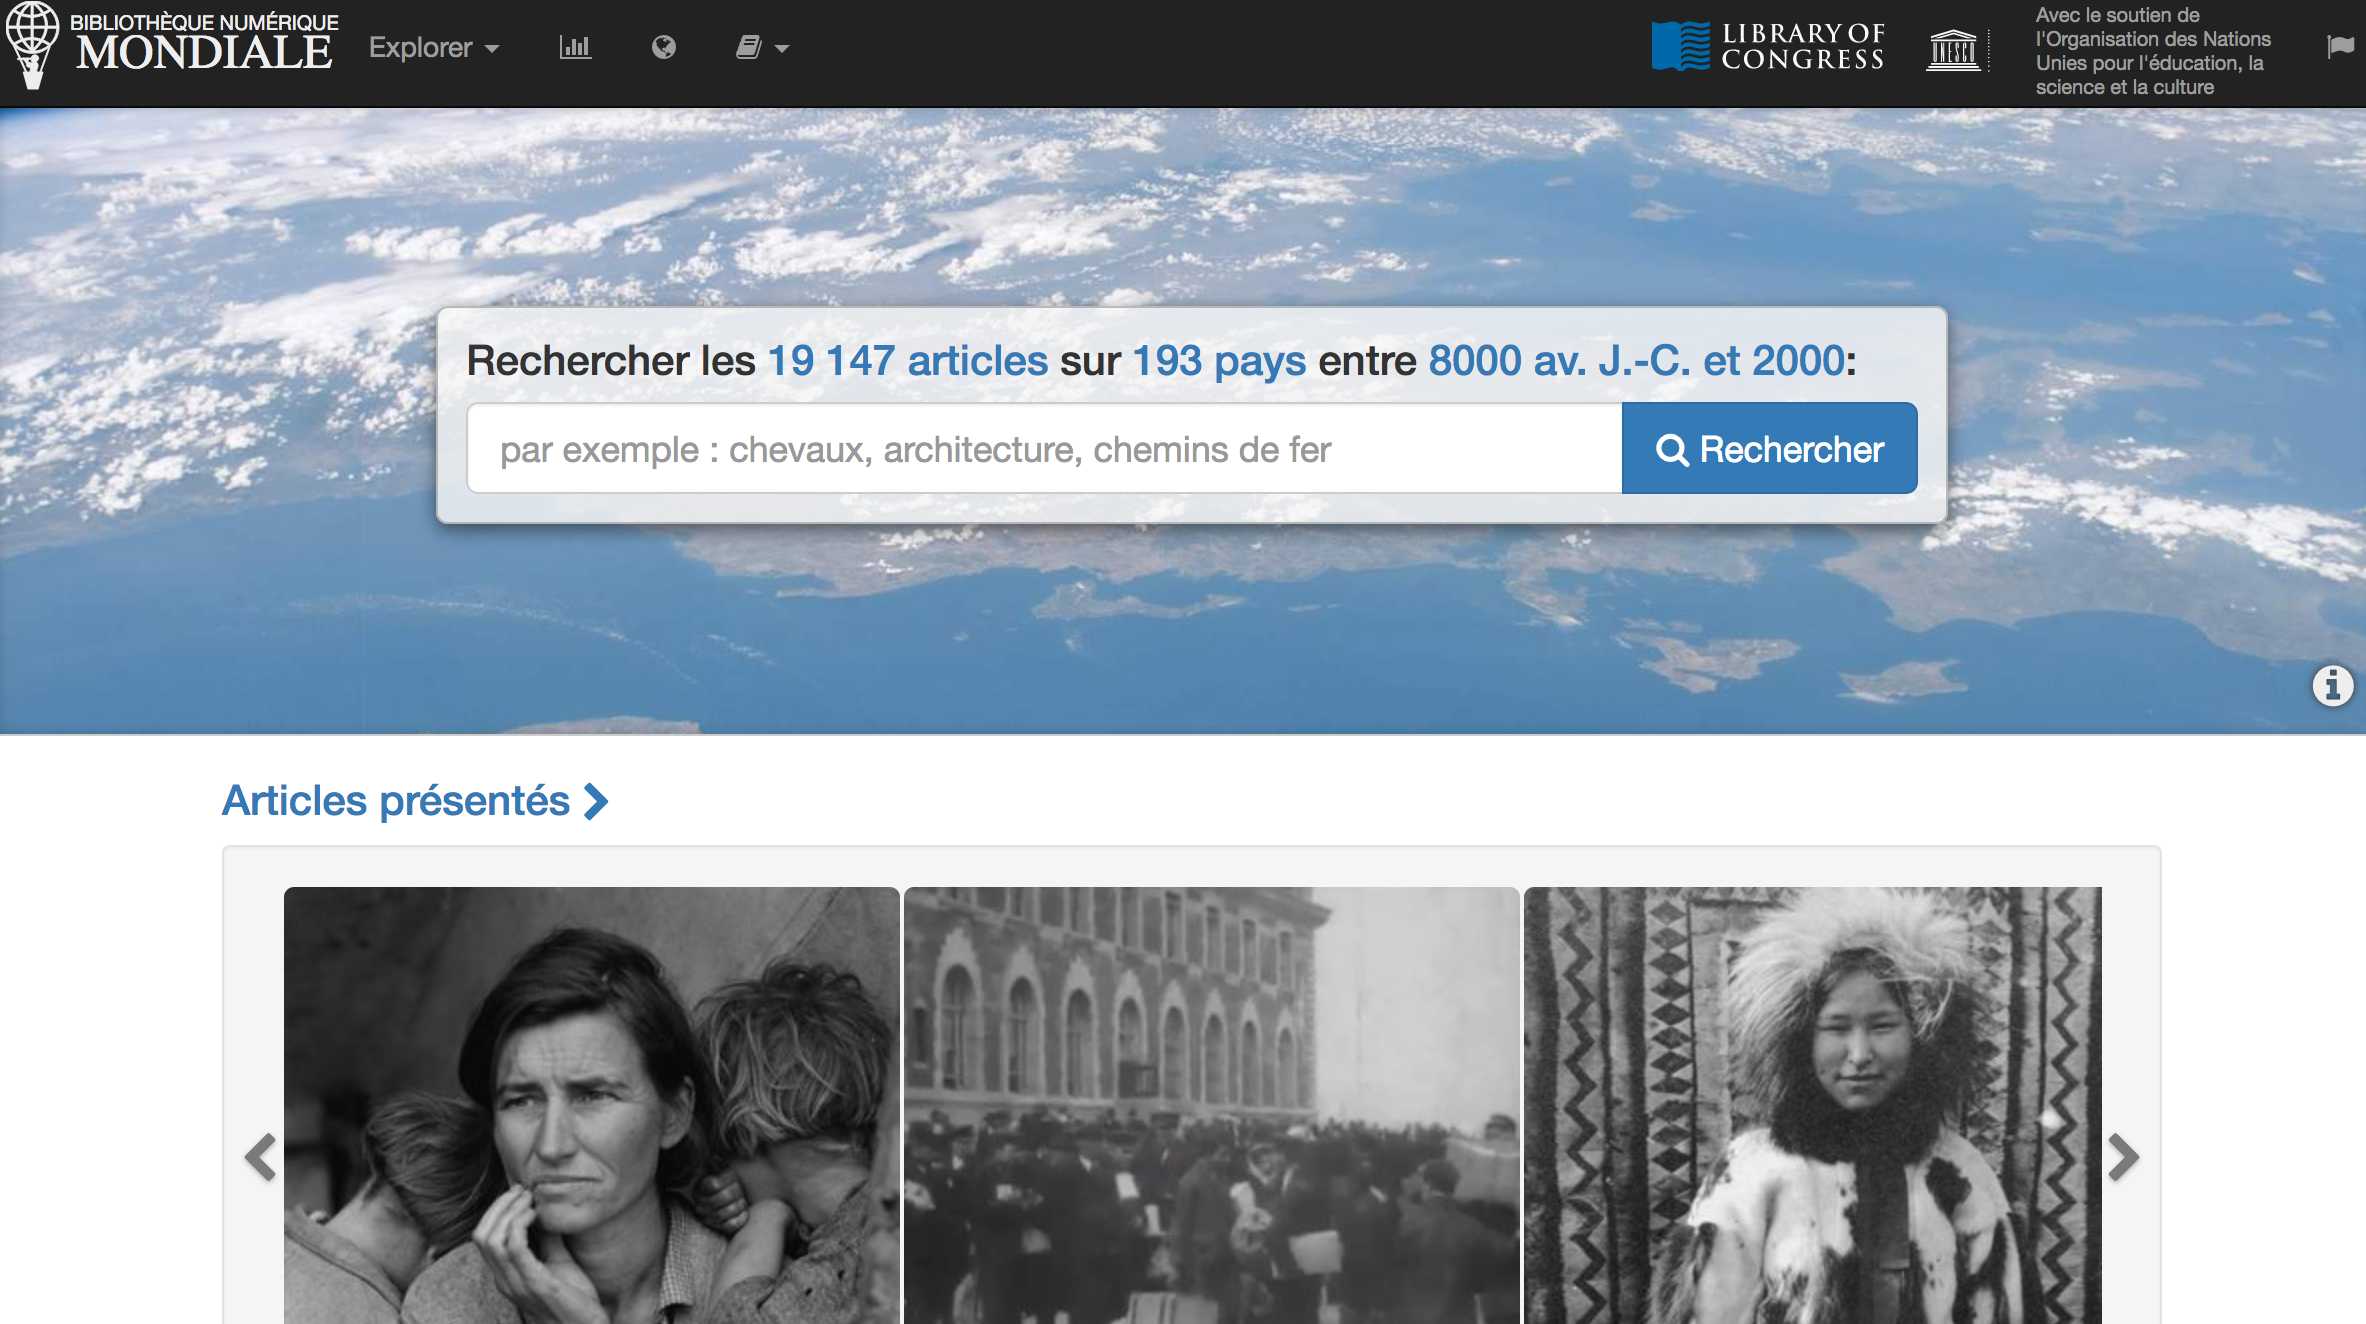
\includegraphics[width=15cm]{unesco}
\caption{Capture-d'écran de la plateforme du projet de Bibliothèque numérique mondiale.}
\end{figure}

La révolution numérique a fortement ébranlé l'\gls{ue} qui, par crainte de manquer ce tournant économique, énonce en 2010 diverses mesures dans son agenda Europe 2020, dont une spécifiquement consacrée à la numérisation du patrimoine culturel européen à travers Europeana\footnote{\cite{coutts_stepping_2017}}. Cet objectif, loin d'être nouveau, incarne l'évolution d'une volonté politique qui remonte à 2001. Retour sur l'histoire de ces principales actions politiques soutenant les entreprises de numérisation :

Les principes de Lund, définis en 2001, invitent les états membres à collaborer pour proposer un alignement de leurs programmes de numérisation, afin de favoriser la valorisation du patrimoine numérique et l'émergence d'une nouvelle forme d'économie\footnote{\cite{foulonneau_recherche_2003}}.

Consciente des nombreuses barrières technologiques à la mise en place d'une numérisation à l'échelle européenne et au développement d'un marché économique, l'\gls{ue} s'intéresse également à l'interopérabilité et publie en 2002 un rapport sur les bonnes pratiques, \textit{DigiCULT : paysages technologiques pour l'économie culturelle de demain, Faire connaître la valeur de l'héritage culturel}  \footcite{salzburg_research_forschungsgesellschaft_digicult_2002}\footcite{thylstrup_politics_2018}. 
 
Ces principes s'incarneront sous plusieurs formes : le programme MINERVA\footnote{MINERVA vise à mettre en place un réseau de soutien politique pour harmoniser les entreprises de numérisation visant à proposer notamment, des recommandations pour les métadonnées et l'interopérabilité des plateformes. \cite{claerr_manuel_2011}.} en 2003, \textit{The European Library}\footnote{Bibliothèque numérique servant de portail à différentes bibliothèques nationales et qui servira d'\gls{agr} de contenus pour la future Europeana, avant que le projet ne soit gelé en 2016.} en 2005 et Europeana en 2008\footnote{\cite{coutts_stepping_2017}}, et serviront de base pour définir le cadre politique et l'édition d'un certains nombres de recommandations\footnote{\cite{noauthor_commission_2011}}. Certains autres projets furent initiés par l'\gls{ue} durant ces mêmes années à l'instar de MICHAEL \textit{Multicultural Inventory of Cultural Heritage in Europe}, poursuivant des buts similaires et contribuant à rendre parfois trop touffu l'organigramme des initiatives\footnote{\cite{association_pour_le_patrimoine_naturel_et_culturel_du_canton_de_vaud_patrimoine_2012}}. Afin de clarifier les choses, l'\gls{ue} a choisi de concentrer ses forces dans la plateforme d'Europeana.

La Commission européenne publie en 2011 des \textit{COMMISSION RECOMMENDATION on the digitisation and online accessibility of cultural material and digital preservation}, qui précisent notamment que : 
\begin{itemize}
\item La numérisation du patrimoine culturel européen comprend les objets imprimés, les photographies, collections des musées, documents d'archives, sons, documents audiovisuels, monuments et sites archéologiques.
\item Pour couvrir les coûts élevés de la numérisation, des partenariats public-privé doivent être mis en place.
\item Numériser est une manne économique, puisque ces données permettront aux industries créatives et culturelles de proposer de nouvelles formes de services et les aideront dans cette phase de transition liée à la révolution numérique. Il est urgent d'agir sous peine de manquer cette transformation numérique des industries : \inquote{\textit{If Member States do not step up their investments in this area, there is a risk that the cultural and economic benefits of the digital shift will materialise in other continents and not in Europe}.\footnote{\cite{noauthor_commission_2011}}} 
\item Pour diminuer les coûts, il est important d'améliorer les infrastructures techniques existantes et de collaborer à l'échelle européenne pour la mise en place des meilleures solutions.
\item Certaines législations doivent être adaptées pour répondre aux besoins d'échanges et d'interopérabilité de ces initiatives. Lever ces barrières doit être fait sur le plan national et européen pour garantir un degré d'uniformisation. 
\item La conservation des données numérisées doit être faite sur le long-terme.
\item Mettre en place des bases de données favorisant l'identification des \oe{}uvres sous droit d'auteur et faciliter leurs numérisations.
\end{itemize}
Ces recommandations spécifient également que le projet Europeana doit parvenir à numériser 30 millions d'objets d'ici 2015, afin de parvenir à la numérisation de l'intégralité de l'héritage culturel d'ici à 2025\footnote{\cite{coutts_stepping_2017}}.

Faisant suite aux recommandations de la Commission, la directive sur certains usages des \oe{}uvres dites orphelines, datée d'octobre 2012\footnote{Les \oe{}uvres orphelines sont des \oe{}uvres protégées par le droit d'auteur, mais dont le détenteur des droits ne peut être identifié.}, vise à permettre la numérisation des \oe{}uvres sous droit, si certains conditions sont remplies. Une fois qu'une recherche sérieuse des détenteurs des droits a été menée, une base de donnée permet de les enregistrer avant de procéder à leurs numérisations\footnote{\cite{noauthor_orphan_nodate}} .

En 2015, l'\gls{ue}, consciente que la révolution numérique a rétabli des barrières que les politiques européennes s'étaient efforcées de réduire dans le monde physique, notamment concernant la libre circulation des données, inhérente à la réussite de tout projet de numérisation de masse, propose la mise en place d'un marché unique numérique\footnote{\cite{hoekstra_proposed_2019}}. L'idée est de pouvoir ainsi concurrencer les leaders mondiaux qui bénéficient eux-mêmes de vastes marchés économiques\footnote{\cite[p.3]{viola_vers_2017}} en se dotant des moyens pour moderniser et décloisonner cette présence numérique\footnote{\cite{viola_vers_2017}}. Pour pouvoir proposer un meilleur accès, sans frontières, aux commerces en ligne, il faut notamment lever le principe de géolocalisation et moderniser les lois sur le droit d'auteur\footnote{\cite{noauthor_eu_2015}}. Le marché unique numérique est pensé pour aider l'\gls{ue} à rattraper son retard économique.

\begin{quotation}
[\textit{Traduction}]
L'\gls{ue} est très en retard par rapport à d'autres pays et régions concernant les échanges commerciaux en ligne, les compétences numériques, la mise en place de règlements appropriés et l'investissement dans les infrastructures numériques. Cela est unanimement reconnu comme une conséquence d'un marché unique très fragmenté qui entrave les échanges commerciaux numériques entre pays européens et gêne le développement de jeunes plateformes européennes et start-ups.
\footnote{\inquote{\textit{The EU is still lagging far behind other countries and regions when it comes to digital cross-border trade, digital skills, innovative regulation and investment in digital infrastructure. It is widely acknowledge that this is to a large extent the result of a fragmented Single Market, which hinders digital trade between EU-countries and hampers the scaling of young European digital platforms and start-ups}}\cite{dittrich_balancing_2017}.}
\end{quotation}

Les résultats de la mise en place de ce marché tardent à se faire sentir et certains auteurs argumentent que plutôt que de libéraliser, les propositions sont venues ajouter une couche de régulation administrative supplémentaire aux initiatives numériques\footnote{\cite{noauthor_next_nodate}}. Certains s'accordent à dire que l'\gls{ue} s'est trompée de combat et plutôt que d'accroître la compétitivité par ce marché unique numérique, elle devrait s'attaquer aux véritables barrières qui se trouvent dans les lois sur le droit d'auteur, trop souvent envisagées uniquement du point de vue des créateurs de l'\oe{}uvre, voir plutôt de celui des détenteurs des licences\footnote{\cite{schroff_politics_2018}}.

Le nouvel agenda pour la culture, publié en mai 2018, est construit sur l'idée du marché numérique unique, et s'engage à mettre en place un réseau de centres de compétence à travers l'\gls{ue} afin de préserver le patrimoine bâti par le biais de la numérisation de masse, et renforcer la collaboration entre acteurs culturels, industries créatives, autorités locales, partenaires sociaux, instituts de recherche et d'éducation, autour des initiatives de numérisation\footnote{\cite{drennan_european_2018}}. 

L'\gls{ue} s'intéresse de près à l'évolution de ces entreprises de numérisation. La Commission européenne a publié en 2018 un rapport sur cette progression, \textit{European Commission report on Cultural Heritage: Digitisation, Online Accessibility and Digital Preservation}\footnote{\cite{noauthor_european_2019}}. Avec pour objectif d'évaluer les progrès réalisés concernant l'application des recommandations de 2011, il propose un état des lieux des entreprises de numérisation au sein des pays membres et établit certaines bonnes pratiques\footnote{\cite{noauthor_council_nodate}}. Parmi les faits à relever :  un tiers des états font usage de la numérisation et de la 3D pour la préservation du patrimoine, bien qu'il y ait encore un manque de connaissances pratiques constaté dans les milieux professionnels ; un accroissement des partenariats public-privé est observé, pour mieux faire face aux coûts élevés de ces entreprises ; il est complexe d'identifier les \oe{}uvres étant du domaine public ; les \oe{}uvres sous droit d'auteur sont très peu représentées au sein des collections et la directive concernant les \oe{}uvres orphelines est peu utilisée car trop chère à déployer\footnote{\cite{noauthor_european_2019}}\footnote{\cite{zeinstra_research:_2016}}.

Signée durant les \textit{Digital Days 2019}, une nouvelle déclaration européenne \textit{the Declaration of cooperation on advancing digitisation of cultural heritage} s'engage à favoriser la coopération pour faire avancer les entreprises de numérisation patrimoniale. Elle s'articule autour de trois axes\footnote{\cite{noauthor_eu_2019}}.
\begin{enumerate}
\item La mise en place d'une initiative européenne pour avancer la numérisation 3D des monuments, sites et artefacts culturels et patrimoniaux.
\item L'usage de ces ressources numériques pour développer l'engagement citoyen et favoriser l'émergence d'entreprises innovantes dans tous les secteurs.
\item Encourager les initiatives entre partenaires de secteurs et pays différents pour augmenter la capacité de développement de cette numérisation de masse de l'héritage culturel.
\end{enumerate}
Il est intéressant de spécifier que le projet Time Machine est cité par la déclaration comme projet répondant à ces objectifs.

Consciente que les enjeux sont du côté de la gestion des droits des \oe{}uvres numériques, l'\gls{ue} a adopté la \textit{Directive on open data and the re-use of public sector information} en avril 2019. Cette dernière spécifie que les \oe{}uvres libres de droit numérisées doivent demeurer libres de droit. Si un droit exclusif pour numériser ou reproduire une \oe{}uvre est imposé, il ne doit pas excéder une période de dix ans et être au maximum non contraignant. \inquote{\textit{Any licences for the re-use of public sector information should in any event place as few restrictions on re-use as possible, for example limiting them to an indication of source.}}

L'accélération du rythme de publication des recommandations et des directives, semble indiquer que l'\gls{ue} a de hautes attentes, concernant la numérisation de son patrimoine. L'incendie récent survenu à Notre-Dame de Paris est venu encore renforcer un débat déjà existant\footnote{\cite{noauthor_european_2019}}. Europeana ayant dépassé ses objectifs de quantité, l'\gls{ue} semble désormais choisir la voie du développement de la qualité (multilinguisme, plateforme, amélioration de la médiation du contenu etc.)\footnote{\cite{noauthor_european_2019}}.

\begin{figure}[H]% force à placer l'image au sein de notre balise figure
%\centering
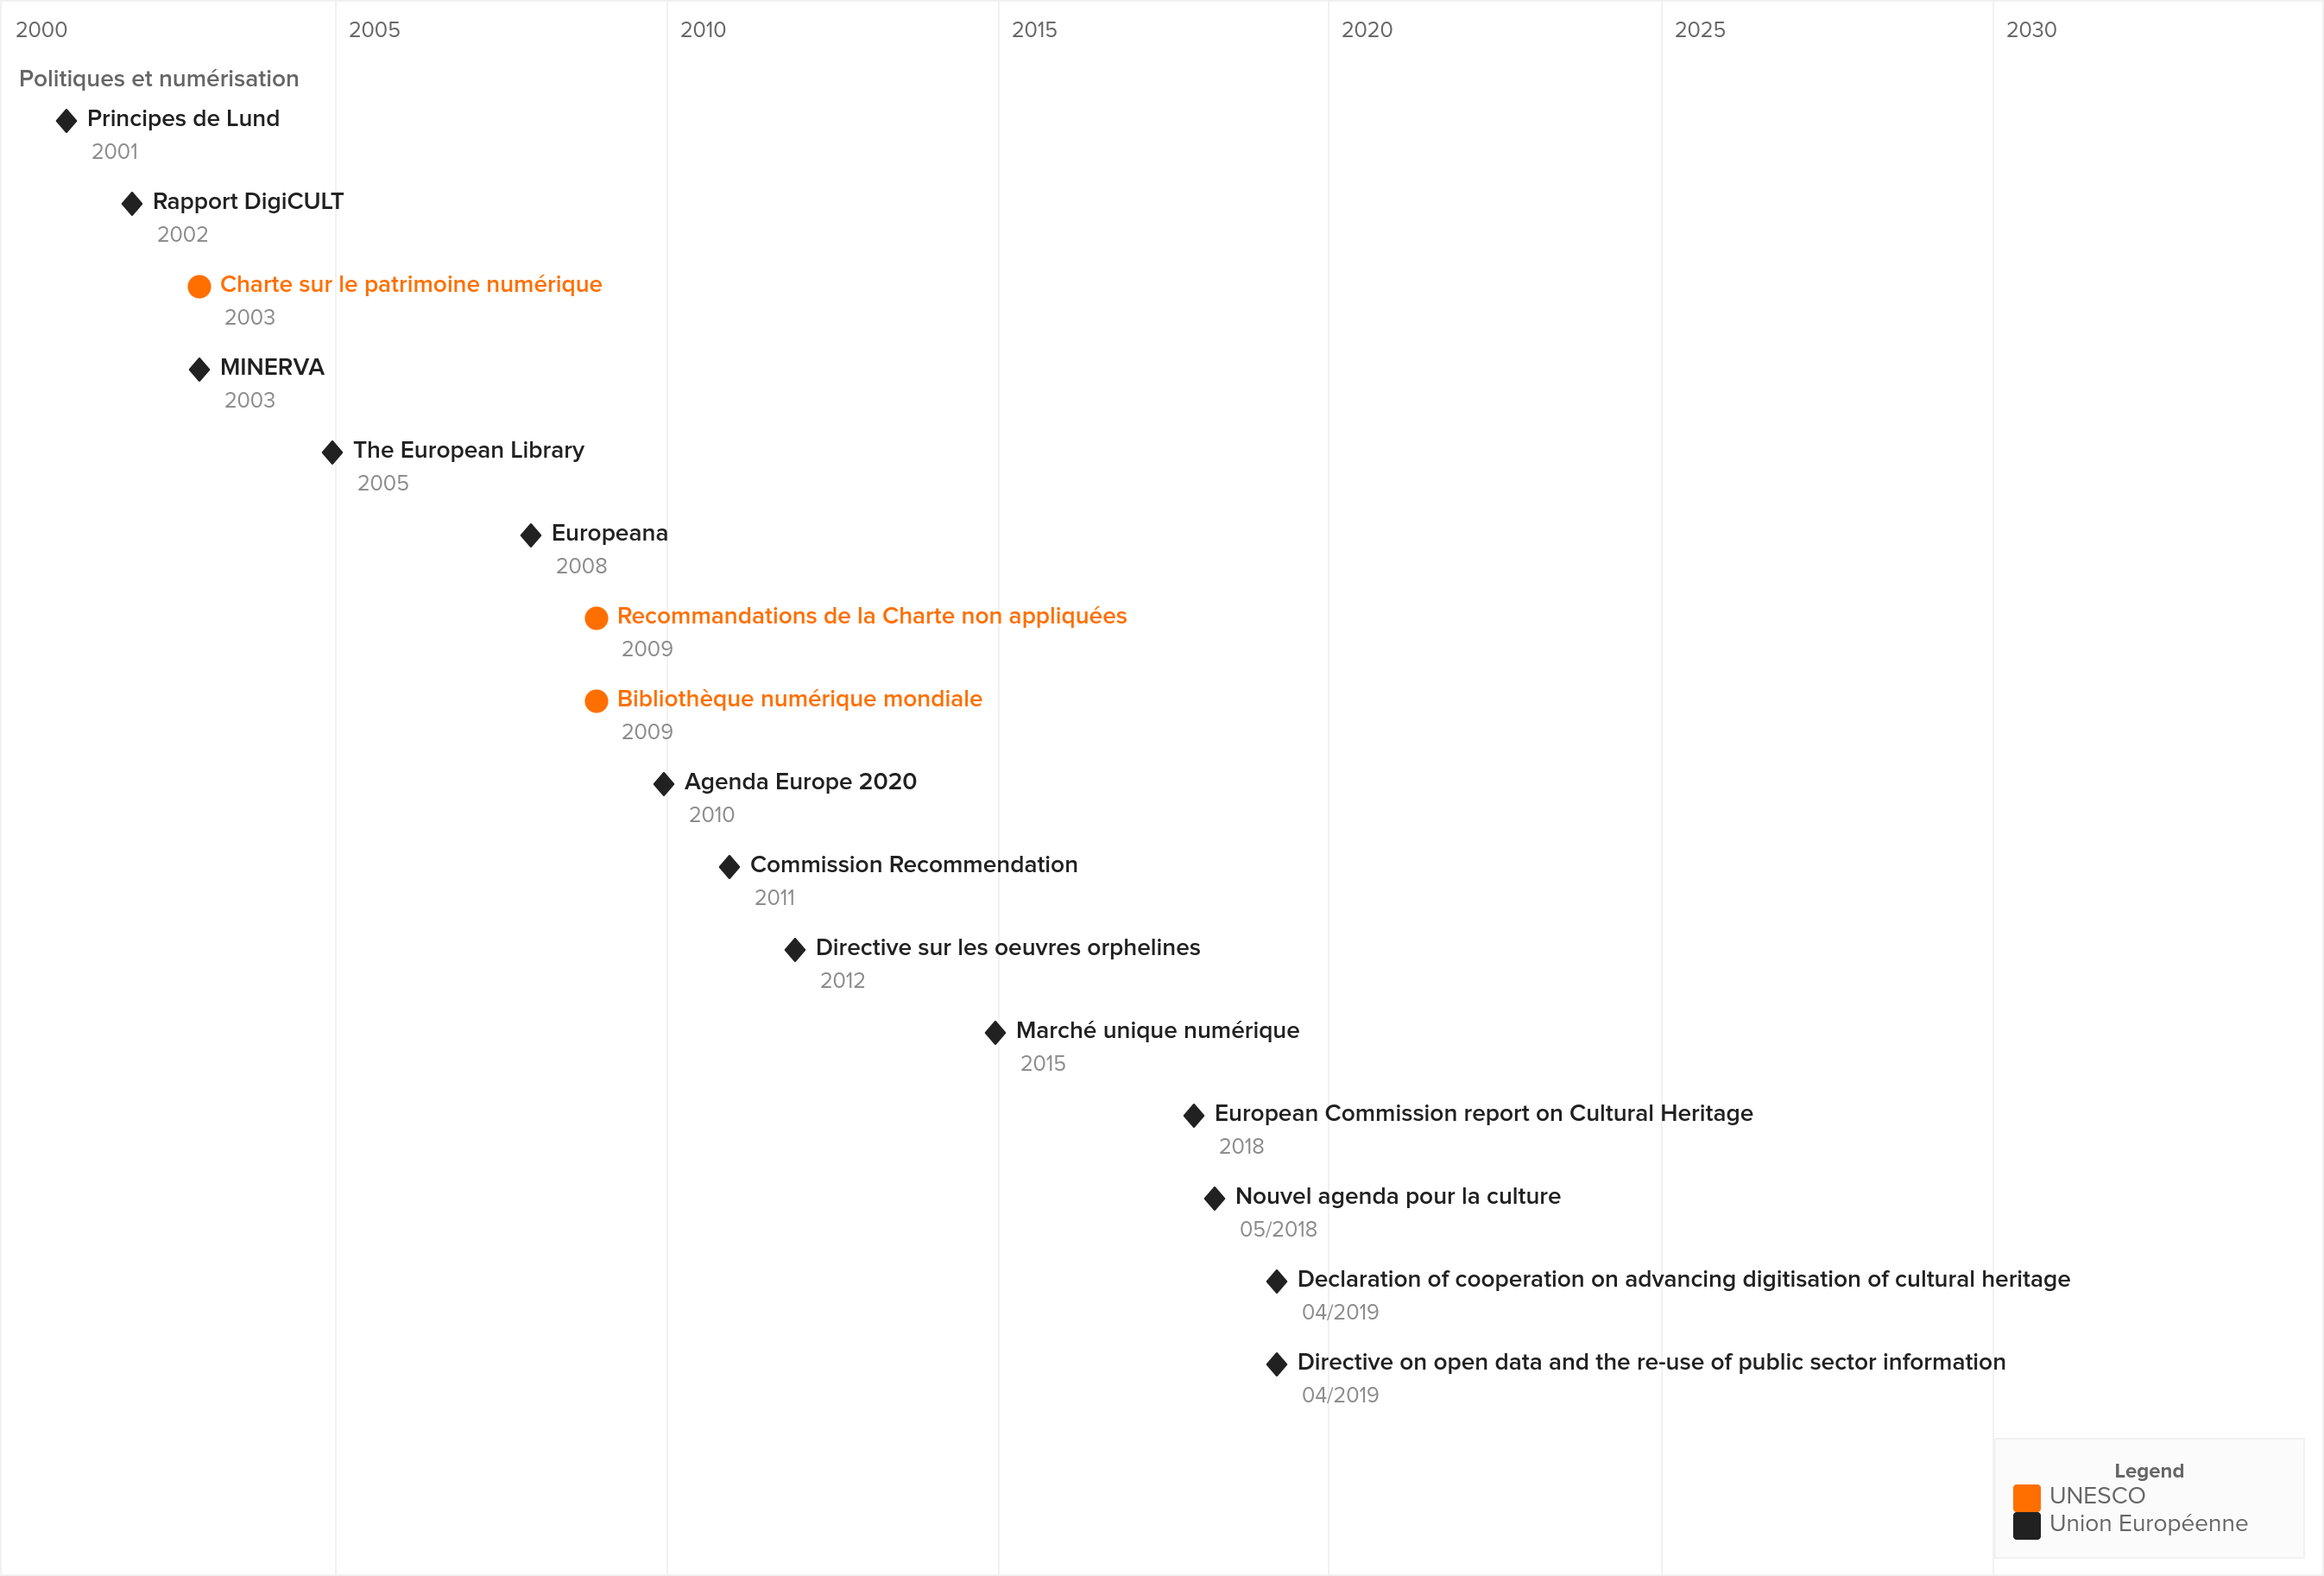
\includegraphics[angle=90, scale=0.27]{politiques_numerisation.png}
\caption{Frise temporelle, \textit{Politiques et numérisation}.}
\end{figure}
\newpage

%========TABLEAU LEçONS
\section{Leçons d'histoire pour Time Machine}

De cette revue du contexte historique, nous avons déduit certaines \inquote{leçons}. %éléments appelés à impacter le futur projet Time Machine. %Nous vous proposons à la page suivante un tableau résumant ces \inquote{leçons de l'histoire}.

\begin{table}[H]
\centering
%

\begin{tabular}{|l|l|lll}
\cline{1-2}
\cellcolor[HTML]{2E1A46}{\color[HTML]{FFFFFF} \textbf{\begin{tabular}[c]{@{}l@{}}Contexte \\ historique\end{tabular}}}    & \cellcolor[HTML]{2E1A46}{\color[HTML]{FFFFFF} \textbf{Points d'attention pour Time Machine}}                                                                                                                                                               &  &  &  \\ \cline{1-2}
{\color[HTML]{2E1A46} }                                                                                                   & Le projet de bibliothèque universelle n'est pas nouveau.                                                                                                                                                                                                   &  &  &  \\ \cline{2-2}
{\color[HTML]{2E1A46} }                                                                                                   & \begin{tabular}[c]{@{}l@{}}Les développements technologiques impactent la portée et le cadre \\ des projets.\end{tabular}                                                                                                                                  &  &  &  \\ \cline{2-2}
\multirow{-3}{*}{{\color[HTML]{2E1A46} \textbf{\begin{tabular}[c]{@{}l@{}}Prémisses \\de la \\numérisation\end{tabular}}}} & \begin{tabular}[c]{@{}l@{}}La version numérique n'est pas parfaitement identique à la version\\ physique du document.\end{tabular}                                                                                                                         &  &  &  \\ \cline{1-2}
{\color[HTML]{2E1A46} }                                                                                                   & Pas de définition figée pour les projets de numérisation de masse.                                                                                                                                                                                         &  &  &  \\ \cline{2-2}
{\color[HTML]{2E1A46} }                                                                                                   & \begin{tabular}[c]{@{}l@{}}Les collections numériques ne sont pas le reflet de la connaissance \\ universelle et portent des biais hérités des collections physiques et\\ motivés par leurs sources de financement.\end{tabular}                           &  &  &  \\ \cline{2-2}
{\color[HTML]{2E1A46} }                                                                                                   & \begin{tabular}[c]{@{}l@{}}Différents acteurs impliquent différents intérêts qui se mêlent au sein \\ d'un projet. Point de vue technologique, point de vue patrimonial, \\ point de vue du public ; partenaires publics, partenaires privés.\end{tabular} &  &  &  \\ \cline{2-2}
{\color[HTML]{2E1A46} }                                                                                                   & \begin{tabular}[c]{@{}l@{}}La construction d'une collection numérique peut être définie par des \\ choix politiques.\end{tabular}                                                                                                                          &  &  &  \\ \cline{2-2}
{\color[HTML]{2E1A46} }                                                                                                   & \begin{tabular}[c]{@{}l@{}}La taille du projet induit un besoin de standardisation et la mise en \\ place de bonnes pratiques.\end{tabular}                                                                                                               &  &  &  \\ \cline{2-2}
{\color[HTML]{2E1A46} }                                                                                                   & \begin{tabular}[c]{@{}l@{}}Ouverture et protection du droit d'auteur ne sont pas synonymes, et \\ les enjeux légaux réels.\end{tabular}                                                                                                                    &  &  &  \\ \cline{2-2}
\multirow{-7}{*}{{\color[HTML]{2E1A46} \textbf{\begin{tabular}[c]{@{}l@{}}Passage à \\ l'échelle\end{tabular}}}}          & \begin{tabular}[c]{@{}l@{}}Le projet se construit pour être au service de l'utilisateur final et \\peut être influencé par ce dernier.\end{tabular}                                                                                                       &  &  &  \\ \cline{1-2}
{\color[HTML]{2E1A46} }                                                                                                   & La numérisation est au programme des politiques européennes.                                                                                                                                                                                               &  &  &  \\ \cline{2-2}
{\color[HTML]{2E1A46} }                                                                                                   & Il y a une volonté d'aligner les initiatives.                                                                                                                                                                                                  &  &  &  \\ \cline{2-2}
{\color[HTML]{2E1A46} }                                                                                                   & Des partenariats public-privé servent à financer les projets.                                                                                                                                                                                            &  &  &  \\ \cline{2-2}
{\color[HTML]{2E1A46} }                                                                                                   & \begin{tabular}[c]{@{}l@{}}Les données numérisées permettent l'émergence d'un nouveau secteur \\ économique.\end{tabular}                                                                                                                                  &  &  &  \\ \cline{2-2}
{\color[HTML]{2E1A46} }                                                                                                   & \begin{tabular}[c]{@{}l@{}}Les législations concernant le droit d'auteur doivent être adaptées et \\ uniformisées.\end{tabular}                                                                                                                            &  &  &  \\ \cline{2-2}
{\color[HTML]{2E1A46} }                                                                                                   & Les données numérisées doivent être conservées sur le long-terme.                                                                                                                                                                                          &  &  &  \\ \cline{2-2}
{\color[HTML]{2E1A46} }                                                                                                   & \begin{tabular}[c]{@{}l@{}}Renforcer la coopération autour des entreprises numériques est dans\\ l'agenda européen.\end{tabular}                                                                                                                           &  &  &  \\ \cline{2-2}
{\color[HTML]{2E1A46} }                                                                                                   & Numériser inclut le patrimoine bâti, avec l'aide  de la 3D.                                                                                                                                                                                                &  &  &  \\ \cline{2-2}
\multirow{-9}{*}{{\color[HTML]{2E1A46} \textbf{\begin{tabular}[c]{@{}l@{}}Politiques et \\ numérisation\end{tabular}}}}   & Les œuvre libres de droit doivent le demeurer, une fois numérisées.                                                                                                                                                                                        &  &  &  \\ \cline{1-2}
\end{tabular}
\centering
\caption{Leçons d'histoire pour Time Machine}
\end{table}

%====================CHAPITRE 2 keyword : enjeux

\chapter{\textit{Comment} numériser en masse}

L'histoire des projets de numérisation a permis de mettre en lumière la complexité et la diversité de ces entreprises, s'inscrivant à la fois dans une forme de rupture et de continuité avec ce qui a précédemment été. Si de nombreux scientifiques s'intéressent au \textit{comment} (quelles réponses apporter aux défis techniques, légaux etc. ?) des projets de cette envergure, peu osent s'attaquer au \textit{pourquoi} (quelles formes de connaissance sont créées par ces projets, quels sont les impacts sur l'organisation des entreprises culturelles, de quel contexte politique sont-ils issus, etc. ?)\footnote{\cite{thylstrup_politics_2018}}. Les projets ne se laissent pourtant pas facilement restreindre à des aspects opérationnels et techniques, alors même que ces derniers sont déjà très nombreux et impliquent la définition de nombreuses typologies de standards : 

\begin{quotation}
[\textit{Traduction}]
Ces projets de numérisation de masse partagent de nombreuses caractéristiques. Ils impliquent le développement de standards pour une numérisation uniforme et pour les métadonnées techniques et descriptives ; la prise de décisions sur les droits d'utilisation ; le choix des logiciels de stockage, de l'environnement de mise à disposition des ressources et du matériel informatique.
\footnote{\inquote{\textit{These mass digitization projects have many similar characteristics. They require standards for uniform digitization, standards for descriptive and technical metadata, decision on rights and permissions, decisions on software for storage and end-user access, and decisions on hardware and operating environments}}\cite[p.11]{kowalczyk_digital_2018}.}
\end{quotation}

Nanna Bonde Thylstrup ose voir au-delà du \textit{comment}, en argumentant que ce changement de contenant (passage d'informations cloisonnées dans un objet physique à la création de jeux de données) induit la création de nouvelles voies de transmission de la connaissance et la redéfinition des aspects politiques, légaux, financiers associés. Ce qui aboutit à d'inévitables controverses découlant de tant d'intérêts mélangés.

\begin{quotation}
[\textit{Traduction}]
Les méthodes de numérisation de masse, créent de nouvelles formes de connaissances et de nouveaux moyens de la découvrir. Ce qui à première vue semble se limiter à un simple acte de numérisation (la transformation des limites physiques d'un livre, en un jeu de données libre), révèle, si nous le regardons de plus près, un processus complexe, foisonnant de diverses controverses politiques, légales et culturelles.
\footnote{\inquote{\textit{The practice of mass digitization is forming new excuses of knowledge, and new ways of engaging with that knowledge. What at first glance appears to be a simple act of digitization (the transformation of singular books from boundary objects to open sets of data), reveals on closer examination, a complex process teeming with diverse political, legal, and cultural investments and controversies}}\cite[p.1]{thylstrup_politics_2018}}
\end{quotation}

Pour mieux analyser ces projets et oser s'intéresser au \textit{pourquoi} (dans la troisième partie de ce mémoire), il nous faut d'abord présenter leur matière même, ce \textit{comment}. Nous vous présentons dans ce chapitre leurs principales caractéristiques puis certains enjeux qui en découlent\footnote{Ces derniers étant très nombreux et de nouveaux ne cessant d'apparaître, nous ne serions prétendre à une absolue exhaustivité.}. Bien que les projets de numérisation de masse ne se laissent que mal résumer tant leurs complexités et spécificités sont grandes, notre revue de la littérature et notre expérience de stagiaire nous ont permis de définir les problématiques minimales induites par ces initiatives. 

%======= CARACTERISTIQUES DES PROJETS DE NUMERISATION
\section{Caractéristiques des projets}\label{caracteristique}

Avant de tenter une caractérisation des projets de numérisation de masse, rappelons brièvement la signification du terme numérisation. Dans le monde du patrimoine, la numérisation implique traditionnellement\footnote{\cite[p.37]{dufrene_numerisation_2013}} : 

\begin{itemize}
\item La conversion d'un objet physique ou analogique (en général des images, fichiers audio ou vidéo ou du texte) en une suite de données interprétables par des machines.
\item La conversion des catalogues sur fiche des bibliothèques selon le même processus.
\end{itemize}

Le projet Time Machine y ajoute une troisième dimension puisqu'il désigne également : 
\begin{itemize}
\item La transformation du patrimoine bâti ou phénomène géographique en modèles 3D.
\end{itemize}

Dans le cadre de ce mémoire, la définition de la numérisation se veut la plus large possible et peut se résumer par la création d'un contenu, copie ou enregistrement numérique, d'une information analogique contenue par un document, artefact, son, performance, élément géographique ou phénomène naturel.

Au-delà de l'acte lui-même, numériser désigne une série de processus d'analyse intellectuelle et d'indexation visant à satisfaire les besoins des utilisateurs avec, pour double objectif, d'assurer la préservation du document au-delà de la durée de vie de son support et de pouvoir valoriser le document numérisé et son modèle original.\footnote{\cite{noauthor_numerisation_2013}}. Tout projet de numérisation pose une série de difficultés, liées aux coûts souvent élevés, au temps nécessaire pour la réalisation, à la qualité de l'indexation, à la conservation à long-terme des données, au coût induit par la maintenance des équipements informatiques et à la qualification des équipes chargées de gérer la masse des documents numérisés\footnote{\cite[p.37]{dufrene_numerisation_2013}}. 

Les objets choisis pour la numérisation ne sont pas systématiquement le fait de politiques de sélection mais découlent des ressources financières, du temps, de la qualité et des objectifs que l'on veut accomplir : \inquote{\textit{Therefore, looking to our traditional media, digitization is not a question of selection according to certain criteria, but according to financial resources, time line, priorities, quality and/or aims we want to reach.\footnote{\cite[p.19]{association_pour_le_patrimoine_naturel_et_culturel_du_canton_de_vaud_patrimoine_2012}}}}

Karen Coyle définit les projets de numérisation de masse comme la conversion de matériel à une échelle industrielle, sans véritable politique de sélection et utilisant les techniques de \gls{reo} pour permettre les recherches plein-texte : \inquote{\textit{ [...] mass digitization refers to converting materials on an industrial scale without curating specific materials for digitization. OCR is used to make the full text of digitized documents searchable}}\footnote{\cite{coyle_mass_2006}}. 

Iris Xie met en avant leurs plateformes d'accès, en les désignant comme les nouvelles générations de systèmes de découverte, offrant un accès centralisé vers une grande variété du patrimoine culturel et scientifique et caractérisés par plusieurs millions de titres, des formats divers, une politique de gestion du droit d'auteur, une politique de sélection, et des degrés d'accessibilité dérivés en fonction, ainsi que par la mise en place de standards techniques pour assurer l'interopérabilité\footnote{\cite[p.23]{xie_discover_2016}}.

Comme déjà mentionné\footnote{Pour plus de détails, référez-vous à la section \ref{echelle}.}, certains auteurs présentent\footnote{\cite{jones_public_2017}} ou osent une distinction entre les projets menés par des partenaires commerciaux et les projets issus des institutions publiques. Justifié par un enjeu plus grand mis sur l'accessibilité des données dans le premier cas, et par la prise en compte de modération humaine dans la gestion des collections, avec un accent plus développé sur les aspects liés à la préservation des données et la réutilisations des métadonnées existantes dans le deuxième cas. Les objectifs de création d'un moteur de recherche universel et le développement de nouveaux services basés sur l'indexation plein-texte d'immenses corpus de données aux formats divers et issus du domaine public restent communs aux deux types d'initiatives\footnote{\cite[p.47]{lampert_ramping_2018}}. 

Il est toutefois certain que la complexité de tels projets ne saurait faire l'objet d'une seule définition tant les intérêts qu'ils mêlent soulèvent de multiples questions, \inquote{\textit{Mass digitization brings together so many disparate interests and elements that any monotheoretical lens would fail to account for the numerous political issues arising within the framework of mass digitization\footnote{\cite[p.5]{thylstrup_politics_2018}}}}. 

La numérisation de masse semble surtout se distinguer des autres formes de numérisation par une contrainte moins importante sur la sélection des sources et par la vitesse des processus liée aux développements technologiques et à l'automatisation. Ces entreprises ne sont dès lors pas résumables en un tout ou par l'une de leurs parties, elles sont constituées de différents assemblages\footnote{\cite[p.26]{thylstrup_politics_2018}}. Si les projets sont difficiles à catégoriser, ils se regroupent derrière la mission de permettre un meilleur accès aux collections des institutions patrimoniales\footnote{\cite[p.58]{lampert_ramping_2018}}.

Avec l'avènement et la construction de notre société numérique, le développement d'une économie liée et l'arrivée de nouvelles générations, il y a désormais un sentiment d'urgence à numériser le savoir qui motive la poursuite de projets de grande ampleur. Celui-ci fait écho aux premières craintes des informaticiens qui prédisaient que les pratiques des utilisateurs seraient à l'avenir uniquement orientées en ligne.

\begin{quotation}
[\textit{Traduction}]
Dans un contexte d'accroissement de la dominance numérique et puisque la plupart des biens patrimoniaux et culturels existent incontestablement uniquement sous une forme physique, la numérisation demeure comme par le passé, un élément clé de tous futurs développements.
\footnote{\inquote{\textit{In the light of increasing digital dominance, however, and the incontrovertible fact that so much of the world's knowledge and cultural outputs still exist only in physical form, digitisation is as much a key element in future digital developments as it has been in the past}}\cite[p.4]{coutts_stepping_2017}}
\end{quotation}

\begin{quotation}
[\textit{Traduction}]
Il existe aujourd'hui des risques considérables à ne pas faire progresser les projets de numérisation. Les nombreux utilisateurs exclusivement numériques pourraient ignorer, voire ne jamais être informés de l'existence de contenus pertinents pour leurs besoins et intérêts. Une connaissance négligée à travers le temps, devient une connaissance perdue, au détriment de tous.
\footnote{\inquote{\textit{There are considerable risks in not advancing digitisation at this time. The numerous digital-only users may ignore or never know of key content which is relevant to their interests and needs. Neglected knowledge, over time, becomes lost knowledge, to the detriment of all}}.\cite[p.4]{coutts_stepping_2017}.}
\end{quotation}

Cette intensification des projets commence à ouvrir les débats autour des questions du \textit{pourquoi} de la numérisation, et certains auteurs s'attachent à proposer de nouveaux angles d'analyse, interrogeant la typologie des acteurs de la numérisation et les leçons à apprendre de ces initiatives\footcite[p.47]{lampert_ramping_2018}\footnote{\cite{thylstrup_politics_2018}}.

%======= ENJEUX DES PROJETS DE NUMERISATION
\section{Enjeux des projets}
Nous avons choisi de présenter les enjeux qui nous ont semblés incontournables pour toute entreprise de numérisation, cependant le développement rapide de ces initiatives et des technologies numériques, nous interdit de prétendre être exhaustive. Ces derniers se construisent autour des questions liées à la mise en place d'une collaboration effective entre différents partenaires, au coût, au droit d'auteur, à l'interopérabilité découlant de choix techniques ou de la construction des corpus, ainsi qu'à la préservation et au stockage de ces données. Ces différents axes interagissent les uns avec les autres au sein d'un même projet, et les décisions relatives peuvent influencer sa réussite finale. 
L'arrivée de \textit{Google Books} a fortement impacté les stratégies des projets de numérisation et semble être l'origine de la nouvelle complexité de ces enjeux\footcite{dufrene_numerisation_2013}.

Les réponses apportées par certaines initiatives et par Time Machine à ces enjeux du \textit{comment} seront examinées respectivement dans la deuxième et la troisième partie du mémoire.
%===COLLABORATION
\subsection{Amener différents acteurs à collaborer }
Les projets de numérisation de masse ont poussé les bibliothèques à sortir de leur isolement. Pour arriver à une meilleure efficacité et une meilleure \inquote{compétitivité}, il a fallu travailler à inscrire la numérisation du patrimoine dans les objectifs de politique publique, définir plus précisément la notion d'Europe culturelle déjà existante dans l'agenda européen\footnote{Pour plus de détail référez-vous à la section \ref{politique}.}, agrandir l'offre à d'autres objets que les livres et partager les infrastructures existantes. Ce qui a conduit les \gls{glam}s à vouloir davantage coopérer au sein d'un même projet\footcite{dufrene_numerisation_2013}. 

\begin{quotation}
[\textit{Traduction}]
Les bibliothèques et archives sont très conscientes des opportunités offertes par la collaboration en regard de ce qui pourrait être fait en travaillant seul. Nous constatons une grande volonté de leur part à développer de telles initiatives. Les bibliothèques publiques et les musées sont les premiers à viser l'amélioration de leurs services au public par le biais de la collaboration et de la mise en commun de collections et d'infrastructures.
\footnote{\inquote{\textit{There is also a strong emphasis on the opportunities to achieve more by working with others than can be achieved by working alone, and this is specified by the library and archives sectors in particular. The public libraries and museums are prominent among those targeting improved public services through collaboration, and in sharing collections and infrastructure}}\cite[p.23]{coutts_stepping_2017}.} 
\end{quotation}

S'inscrivant dans le contexte multilatéral et international de la mondialisation, les projets doivent  orchestrer le double retour du local et du national\footcite[p.175]{dufrene_numerisation_2013}.

La collaboration est également nécessaire pour définir les choix techniques inhérents à la mise en commun des collections de diverses institutions, que les frontières nationales soient dépassées ou non par le cadre du  projet\footcite{moatti_bibliotheque_2012}. 

L'accélération des processus induits par l'envergure du projet implique souvent l'externalisation à un prestataire de certains actes de numérisation et le transport des documents concernés. L'organisation du flux des documents entre l'institution détentrice et le prestataire doit être soigneusement planifiée\footcite{ministere_de_la_culture_et_de_la_communication_:_direction_des_archives_de_france_ecrire_nodate}.

De la qualité de la collaboration découlent la possibilité de coordonner différentes initiatives de numérisation et de proposer une vision globale. Cet aspect semble souvent faire défaut aux initiatives, alors même que la collaboration est susceptible d'impacter fortement tous les autres enjeux\footcite{coutts_stepping_2017}. Parvenir à faire collaborer un nombre croissants de partenaires induit la mise en place d'outils de gestion, la définition d'un cadre, et la prise en compte du multilinguisme, et représente de fait un investissement nécessaire pour la réussite du projet\footcite{eschenfelder_nine_2019}.

\begin{quotation}
[\textit{Traduction}]
Bien entendu, chaque organisation sera confrontée à ses propres limites, et certaines initiatives ne pourront être poursuivies faute d'une collaboration effective mise en place avec soin. Collaborer implique un environnement délicat et finement équilibré [...]. Collaborer signifie travailler avec un ensemble cohérent et complexe de partenaires régionaux, nationaux et internationaux.
\footnote{\inquote{\textit{Ultimately, however, there will be limits to every organisation's options, and there will be initiatives that cannot go forward because they lack the collaborative commitment that they require. Collaboration is a finely balanced and delicate environment [...]. Collaboration means working with a coherent and complex set of regional, national, and international partnerships}}\cite[p.26]{coutts_stepping_2017}.}
\end{quotation}

 %===FINANCEMENT
\subsection{Financement et partenariats public-privé}

Les coûts élevés de la numérisation de masse et les limitations posées par le système de numérisation à la demande\footcite{maurel_quel_2017}\footnote{En général, le premier utilisateur paie pour le processus, le fichier est ensuite publié si libre de droit, sur la plateforme de l'institution.}, ont poussé les initiatives à chercher des solutions du côté des partenaires privés (individus, banques, fondations, médias, industries du tourisme etc.)\footcite{lopatin_library_2006}\footcite{yeates_collaborative_2006}. En général, comme les coûts sont fortement imputés à l'infrastructure\footnote{De grands progrès ont toutefois été faits sur les couches technologiques, la montée des coûts serait due aux recherches pour les droits d'auteur. \cite{stobo_i_2018}.}, ce sont vers des entreprises spécialisées dans ces technologies (à l'instar de Google, Proquest, IBM, Kodak)\footcite{dufrene_numerisation_2013}, que se tournent les institutions culturelles et patrimoniales. On trouve toutefois des engagements avec des fondations telles que Wikimedia et le recours au financement participatif ou \textit{crowdfounding}\footcite{noauthor_european_2019}\footnote{Cette piste demeure ambiguë, car pose des problèmes de réutilisation commerciale des \oe{}uvre ainsi numérisées. \cite{maurel_quel_2017}.}. 

L'arrivée des ces partenariats privés a reçu un accueil au départ très mitigé par crainte d'un monopole et de la réappropriation des ouvrages libres de droit publiés sous licence\footnote{Voir aussi à ce propos dans la section \ref{politique} la récente directive de l'\gls{ue}, sur les ouvrages libres de droit.}\footcite{association_pour_le_patrimoine_naturel_et_culturel_du_canton_de_vaud_patrimoine_2012}. Ces partenariats financiers entre institutions publiques et prestataires privés posent également des problèmes liés à la réutilisation des données, puisque certains prestataires imposent des conditions d'exclusivité\footcite{dufrene_numerisation_2013}\footnote{Voir aussi à ce propos dans la section \ref{politique} la récente directive de l'\gls{ue}, visant à limiter la durée des périodes d'exclusivité.}. De récentes études montrent toutefois que l'exclusivité tend à ne plus porter directement sur l'utilisation des oeuvres numérisées mais se déplace vers la commercialisation de services\footcite{maurel_quel_2017}.

En dépit de la prolifération de ces partenariats, il manque un socle de règles communes visant à limiter les risques de monopole de certains acteurs privés et à fixer un cadre permettant d'harmoniser et légitimer ces pratiques\footcite{dufrene_numerisation_2013}, afin de trouver l'équilibre entre des financements gouvernementaux, locaux, privés et caritatifs\footcite{yeates_collaborative_2006}. La mise en place d'une politique active de numérisation dans chaque état pourrait également permettre de rééquilibrer la situation\footcite{maurel_quel_2017}\footnote{Les Pays-Bas ont par exemple mis en place une loterie nationale pour répondre aux besoins financiers des institutions culturelles.}.

Malgré la créativité déployée par les initiatives pour parvenir à couvrir leurs frais, un manque est constaté dans l'organisation des projets, qui ont tendance à négliger la perspective du long-terme. Les projets financés par des bourses locales, nationales ou européennes sont souvent les plus susceptibles de présenter un modèle financier lacunaire\footcite{lampert_ramping_2018}. Ceci conduit à une multiplicité de projets financés, mais plus accessibles car les contenus n'ont jamais été mis à jour et les plateformes datées\footcite{eschenfelder_nine_2019}. 

Très peu d'études s'attachent à analyser le rapport entre l'audience générée par les plateformes et leurs coûts de production, ce qui permettrait aux initiatives de justifier ou d'adapter leurs investissements\footcite{moatti_bibliotheque_2012}.
 %===DROIT D'AUTEUR
\subsection{Droit d'auteur}

Les projets de numérisation de masse suscitent une prise de conscience de l'urgence à ne pas limiter les collections aux ouvrages libres de droit\footcite{dufrene_numerisation_2013}. La question du droit d'auteur devient incontournable, les institutions ayant la responsabilité de déterminer si le droit d'auteur s'applique ou non aux \oe{}uvres qu'elles souhaitent numériser\footcite{lopatin_library_2006}. 

La problématique du droit d'auteur, dans tout projet de numérisation, intervient de différentes manières\footcite{dufrene_numerisation_2013} :
\begin{itemize}
\item Certaines \oe{}uvres sont libres de droits, car dans le domaine public.
\item Certaines \oe{}uvres sont couvertes par le droit d'auteur, mais dites orphelines\footnote{Pour rappel, les \oe{}uvres orphelines sont des \oe{}uvres soumises au droit d'auteur mais dont le détendeur est inconnu.}.
\item Certaines \oe{}uvres existent nativement sous forme numérique et sont couvertes par des licences numériques.
\end{itemize}

Les exceptions au droit d'auteur sont réglées par un certain nombre de régimes de droits nationaux et quelques directives européennes visant à faciliter leur gestion. Il n'existe pas, en Europe, de réel équivalent aux exceptions définies par le \textit{fair use}\footnote{Le \textit{fair use} autorise cinq exceptions au droit d'auteur : le droit à opérer une copie privée, le droit de citation, le droit au pastiche ou à la caricature, l'usage pour l'enseignement, l'usage pour la recherche.} états-unien, qui a notamment servi à justifier la pratique de \textit{Google Books}. L'\gls{ue} est toutefois consciente des enjeux liés au droit d'auteur et a mis en place un certain nombre de recommandations et de directives\footnote{Pour plus de détail, référez-vous à la section, \ref{politique}}.

La montée des coûts des entreprises de numérisation de masse se justifie de plus en plus par la recherche des auteurs des \oe{}uvres sous droit\footcite{stobo_i_2018}. En effet dans l'environnement numérique, les détenteurs des droits ont un contrôle presque absolu sur l'utilisation de l'\oe{}uvre originale\footcite{pavlovic_serpent_2011}. Les détenteurs de ces droits refusent souvent de libérer les \oe{}uvres et ont peu d'intérêt à réduire les coûts pour les initiatives de numérisation, car cela représente une perte financière\footcite{stobo_i_2018}. Les acteurs cherchent surtout à maintenir un équilibre économique, chèrement acquis par les industries créatives\footcite{stobo_i_2018}. \inquote{\textit{The commercial publishers representing the greatest copyright holders were the most reluctant to grant the permission, fearing loss of their profits\footcite[p.54]{george_testing_2005}.}}

Cette situation conduit à une sous-représentation des \oe{}uvres à partir du 20\up{e} siècle au profit des \oe{}uvres plus anciennes généralement libres de droit, phénomène connu sous le nom de \inquote{Trou noir} du 20\up{e} siècle\footcite{dufrene_numerisation_2013}, \textit{20th century black hole}\footcite{noauthor_european_2019} ou encore \textit{digital black hole}\footcite{association_pour_le_patrimoine_naturel_et_culturel_du_canton_de_vaud_patrimoine_2012}.

Dans le cas des \oe{}uvres dites orphelines, la directive européenne de 2012\footnote{Pour plus de détail, référez-vous à la section, \ref{politique}} permet aux institutions de les numériser, mais impose la poursuite de recherches diligentes et le respect de nombreuses règles (interdiction de les utiliser ensuite pour un usage commercial, etc.) avant le lancement des processus\footcite{stobo_i_2018}. Ce qui s'avère trop coûteux pour la plupart des projets\footcite{noauthor_european_2019}.

Pour les \oe{}uvres encore soumises au droit d'auteur, mais non trouvables dans le commerce, il n'existe aucune directive visant à faciliter la recherche des détenteurs de droit et à lever les coûts imposés par ces derniers\footcite{noauthor_european_2019}.

Il y a un grand besoin de rétablir l'équilibre entre la protection des droits d'auteur et du profit qu'il génère pour certains, et la protection des intérêts du grand public et de la société à utiliser ces \oe{}uvres\footcite{pavlovic_serpent_2011}. Le droit d'auteur doit être adapté aux nouveaux modes de production de la connaissance\footcite{dufrene_numerisation_2013}. 

\begin{quotation} 
[\textit{Traduction}]
Ces dernières années, le droit d'auteur semble avoir dérivé vers une protection des détenteurs du droit au détriment des bénéfices pour la société. Les délégués semblent incapables ou peu disposés à changer cet équilibre par de nouvelles législations. Puisque les règlements existants sont mal équipés pour faire face aux nouvelles technologiques, les riches détenteurs de droits ont prestement utilisé ces nouvelles technologies pour accroître la protection de leurs \oe{}uvres ou intimider les usagers. \footnote{\inquote{\textit{In recent years, the balance of copyright appears to have tipped more toward the rights of copyright owners over the benefits to society, with legislators unable or unwilling to change that balance through new legislation. Because existing statutory language is ill-equipped to handle new technologies, wealthy and powerful copyright holders have been quick to use technology to expand protection of their works or to intimidate users}}\cite[p.54]{xie_discover_2016}.}
\end{quotation}

Solution possible à cette situation paradoxale, le \gls{oa} et l'\gls{os} méritent d'être davantage développés. Les exceptions au droit d'auteur doivent également être davantage explorées par les projets de numérisation de masse dont les institutions craignent trop souvent les retombées légales, ce qui ajouterait la gestion des risques à la liste des enjeux identifiés\footcite[p.661]{stobo_i_2018}. \inquote{Cependant ni la capitulation devant le droit d'auteur ni la transgression provocatrice des règles fondamentales ne peuvent résoudre le problème à la longue\footcite{association_pour_le_patrimoine_naturel_et_culturel_du_canton_de_vaud_patrimoine_2012}.}

\begin{quotation}
[\textit{Traduction}]
Compte tenu des coûts trop élevés associés à la recherche des auteurs des \oe{}uvres orphelines dans le cas de collections de grandes tailles, et du manque d'alternatives législatives, nous proposons que les institutions culturelles et patrimoniales apprennent à vivre en acceptant une certaine forme d'incertitude. Elles doivent explorer les perspectives offertes par une gestion consciente des risques dans leurs stratégies de gestion et mettre à profit le large champ des exceptions prévues dans les législations sur le droit d'auteur.
\footnote{\inquote{\textit{Given the unmanageable transaction costs associated with these orphan works schemes when dealing with collections of any notable size, as well as the lack of other useful cognate legislative form, we argue that Cultural Heritage Institutions must learn to live with the uncertainty inherent in copyright law : that is, they must explore risk management strategies in more depth, and utilise the full scope of the exceptions already available within the copyright regime}}\cite[p.661]{stobo_i_2018}.}
\end{quotation}

 %===SORTIR DES SILOS
\subsection{Sortir des silos - la quête de l'interopérabilité}

Tout projet de numérisation de masse implique à un certain moment, en plus de la \gls{num}, la réunion de collections déjà numériques et la mise à disposition de l'ensemble de ces données à travers une plateforme commune en ligne\footcite{lampert_ramping_2018}. Rassembler ces différentes données, puis les rendre trouvables, est complexe. De trop nombreuses \gls{db} ont été déployées par les institutions, éparpillant les données à travers des systèmes différents et contribuant à les enfermer et les isoler les unes des autres, dans des \inquote{silos}\footcite{institut_national_dhistoire_de_lart_lundisnum_nodate}. 

L'interopérabilité est un argument pour beaucoup, pour l'\gls{ue} qui souhaite mettre en place des procédures communes favorisant l'économie de la connaissance, pour les professionnels des bibliothèques et archives souhaitant sortir de leurs logiques de \inquote{silos} et pour le mouvement de \textit{\gls{os}}. L'objectif de l'interopérabilité est de faciliter les échanges de données entre les différents systèmes des institutions culturelles et patrimoniales\footcite{lopatin_library_2006} et de proposer des services permettant d'accroître les interactions avec ces ressources au sein d'un même réseau\footcite{xie_discover_2016}.

\begin{quotation}
[...] l'interopérabilité est devenue un enjeu à un autre niveau que par le passé. Il ne s'agit plus seulement d'échanger des notices pour éviter la redondance dans l'effort de catalogage, mais de mutualiser les outils à travers des \inquote{portails} pour tenter d'accrocher un usager devenu insaisissable\footcite[p.21]{bermes_web_2013}.
\end{quotation}

Alors que les standards et les bonnes pratiques apportent de nouvelles réponses aux enjeux techniques posés par la numérisation, ces derniers ne semblent pas encore avoir trouvé leur forme finale. 

De plus, un autre écueil contribue à isoler les collections des institutions culturelles et patrimoniales : celui de la sélection du contenu intellectuel. Un manque de coordination et de vision globale sur la création de ces collections les rend fortement disparates et complique davantage leur réunification au sein d'une même plateforme\footcite{coutts_stepping_2017}, augmentant également la redondance des données numérisées\footcite{institut_national_dhistoire_de_lart_lundisnum_nodate}. 

De l'attention apportée aux enjeux  techniques et aux enjeux sur le contenu, découle d'une part la qualité et la richesse de l'expérience proposée ensuite pour utilisateur, et d'autre part la qualité de la conservation sur le long-terme\footcite{xie_discover_2016}. 

Nous n'avons pas pour objectif de définir quelle sont les meilleurs pratiques à adopter, puisque ces dernières sont propres au contexte de chaque projet et liées aux objectifs utilisateurs, mais nous vous proposons une introduction des différents éléments auxquels toute initiative sera amenée à se confronter.

Il n'existe pas encore de modèle de donnée européen ou universel propre à assurer l'interopérabilité. La coopération entre institutions culturelles, professionnels de l'information et utilisateurs est essentielle pour la définition et l'implémentation d'un tel modèle\footcite{rasmussen_pennington_connecting_2019} qui devra être à la foi souple, cohérent et garant de la provenance des données\footcite{institut_national_dhistoire_de_lart_lundisnum_nodate}. Une étude européenne datée de 2004 définit trois critères à la réussite de l'interopérabilité : organisationnel, technique et sémantique\footcite[p.565]{zharova_influence_2015}. 
%\addcontentsline{toc}{subsubsection}{Enjeux techniques}
\subsubsection{Enjeux techniques}

%=== NUMERISATION
Les enjeux techniques se découpent en deux grandes familles. La première est liée aux processus de \gls{num}, ses choix portent sur la qualité des productions numériques et les formats\footnote{Le format désigne la nature d'un document informatique et permet d'identifier le logiciel nécessaire à sa lecture. Chaque fichier porte une extension en trois lettres indiquant le format (par ex. pdf pour les documents)} des fichiers ensuite produits. De cette qualité dépendent surtout la découverte proposée aux utilisateurs\footnote{Par exemple, une image sera accessible en plus ou moins haute résolution, ce qui ralentira ou non le navigateur de l'usager} et la préservation sur le long-terme des données\footnote{Pour plus de détails, référez-vous à la section \ref{preservation}}. Les bonnes pratiques privilégient le choix de formats ouverts (par exemple .tiff ou .png pour les images)\footnote{Un format ouvert par opposition aux formats propriétaires est un un fichier dont le code est accessible et transparent et peut être lu par différents logiciels.}. 

Pour s'assurer de la conformité aux critères de qualité, un contrôle doit être mis en place, faisant partie intégrante du projet. Il ne peut se réduire à une simple étape du processus.\inquote{Suivant les moyens disponibles et le niveau de qualité souhaité, on procédera au contrôle à différents moments de la production}\footcite[p.271]{claerr_manuel_2011}.

Si la recherche de la qualité des produits de la \gls{num} a motivé les premières initiatives, il semble que les projets de numérisation de masse ont appelé à une redéfinition des priorités pour produire plus en allégeant les processus, ce qui ne se fait pas sans difficulté. \inquote{Ansi la non-qualité et la sur-qualité sont des extrêmes à éviter}\footcite[p.271]{claerr_manuel_2011}. La qualité minimale se fixant sur l'usage et non sur les conditions de préservation. Les entreprises de numérisation de masse sont ainsi appelées à faire preuve de flexibilité, en appliquant des critères de qualité différents en fonction des documents\footcite{xie_discover_2016}. 

\newpage
\begin{figure}[H]% force à placer l'image au sein de notre balise figure
\centering
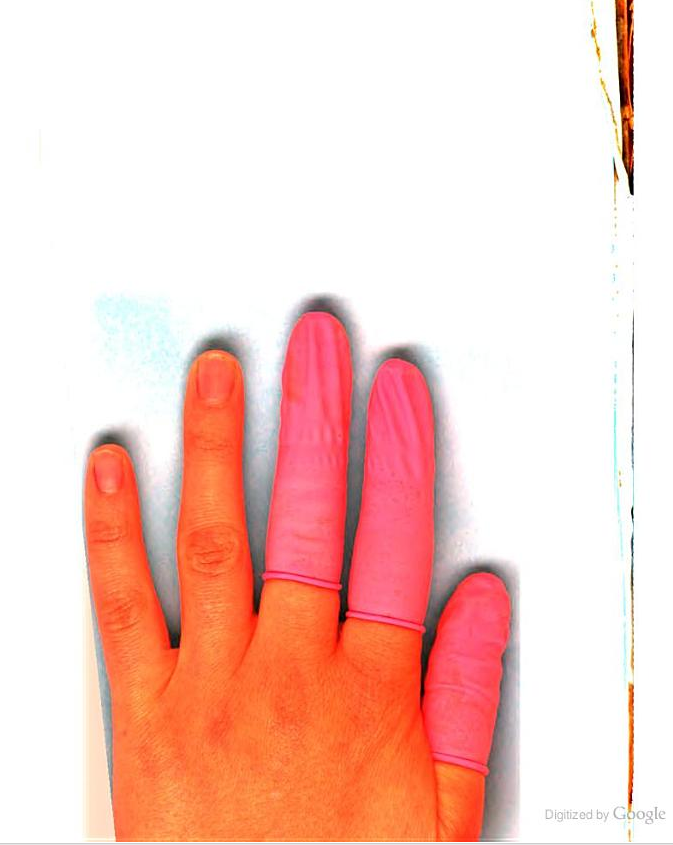
\includegraphics[scale=0.4]{qualite}
\caption{Image de mauvaise qualité, numérisée par Google ©\textit{Google Books}}
\end{figure}


%===METADONNEES

La deuxième famille des enjeux techniques est liée aux données servant à décrire les produits numérisés, soit les métadonnées. La quête de l'interopérabilité permettant de faire communiquer ces corpus de métadonnées décrivant les collections, indépendamment de l'environnement technique de leurs bases de données, est l'une des solutions pour la sortie des silos, ou c'est, en tous les cas, la présomption qui en est faite.

\inquote{\textit{It's a metadata's world, and you're just living in it\footcite[p.4]{pomerantz_metadata_2015}.}} Les métadonnées sont pleinement intégrées dans notre société et passent inaperçues. Nous n'avons pas toujours conscience que lorsque nous achetons un livre en librairie, c'est le titre, l'auteur ou la couverture qui auront motivés notre choix. Les informations servant à décrire le livre ont toujours été utilisées dans les bibliothèques, pour permettre de retrouver et classer les documents et sont à la base des catalogues. Les métadonnées nous servent à simplifier la réalité. Par exemple, \inquote{Camille} est mon prénom, mais ce n'est pas moi en tant que telle. 

Il existe plusieurs catégories de métadonnées, aux frontières parfois un peu floues : les métadonnées descriptives\footnote{Servant à simplifier l'objet ou l'information par le biais de mots-clés.}, les métadonnées administratives\footnote{Informations sur l'origine d'un document, par exemple une photographie numérisée avec tel scanner, telle résolution, sous telle licence}, les métadonnées structurelles\footnote{Informations sur l'organisation de l'objet, par exemple un livre se compose de chapitres.}, les métadonnées de préservation\footnote{Informations spécifiques à la préservation sur le long-terme.}, les métadonnées d'usage\footnote{Informations sur l'usage de l'objet, par exemple combien de fois un livre a-t-il été lu.}\footcite{pomerantz_metadata_2015}. Si les métadonnées descriptives ont été développées avec pour objectif d'améliorer la recherche sur internet, elles n'ont pas longtemps permis de le réaliser. Très vite, des entreprises ont tenté de tromper les moteurs en ajoutant de nouveaux mots-clés, et de fait, ce champ est souvent ignoré. Leur intérêt est néanmoins en train de se réveiller, mais plus pour améliorer l'affichage que pour influencer les résultats d'une recherche\footcite{pomerantz_metadata_2015}. 

La multiplicité des catégories de métadonnées implique la création d'un fichier capable de toutes les contenir : le registre de métadonnées.

L'écriture de ces métadonnées est définie par un certain nombre de règles spécifiant la description de l'élément, on parle alors de schéma de métadonnées. Les schémas sont structurés en triplets : objet (par ex. Camille Besse), prédicat (par ex. est l'auteure), sujet (par ex. du présent mémoire), les règles du schéma servent à spécifier quels prédicats peuvent être utilisés et quelles sortes de déclaration sujet-prédicat-objet sont possibles\footcite{pomerantz_metadata_2015}. La valeur prise par les différentes données du triplet est également normalisée, avec l'aide notamment de vocabulaires controlés\footnote{Lexique servant à organiser les connaissances pour favoriser la recherche d'information} et d'ontologies\footnote{\inquote{Une ontologie est une façon de modéliser un domaine en identifiant les concepts y afférent et en les organisant les uns par rapport aux autres }\cite{delestre_du_2017}.}. \inquote{\textit{If a metadata schema expert control over the kinds of statements that may be made, a controlled vocabulary expert control over the words and phrases that may be used in those statements}.\footcite[p.33]{pomerantz_metadata_2015}}

Bien que les métadonnées soient cruciales pour le succès des entreprises de numérisation de masse\footcite{pomerantz_metadata_2015}, elles ont souvent été développées sans souci d'uniformisation, rendant la situation actuelle très hétérogène\footcite{rasmussen_pennington_connecting_2019}. Les institutions culturelles ne traitent pas leurs métadonnées selon les mêmes schémas (différences notables entre les collections des bibliothèques, des archives, des musées)\footcite{bermes_web_2013}. Nous verrons, dans la deuxième partie de ce mémoire, les exemples d'Europeana et de \textit{The Digital Public Library of America} qui, dans leurs objectifs de rassembler différentes collections, ont créé leurs propres schémas de métadonnées\footcite{pomerantz_metadata_2015}.

Pour pallier à cette hétérogénéité des schémas de métadonnées, le \textit{Semantic Web Education and Outreach Interest Group}, créé en 2006 par le \gls{w3c}\footnote{Communauté internationale chargée de développer les standards du web afin de garantir sa longévité.} a proposé une nouvelle solution visant à faciliter l'échange de ces métadonnées, pour permettre aux machines de les interpréter et construire de nouvelles applications et de nouveaux services\footcite{bermes_web_2013}. S'exprimant à travers les technologies du web sémantique, le web de données est définit comme : 

\begin{quotation}
[...]un réseau où les données structurées qui se trouvent actuellement isolées dans les bases de données pourraient être exprimées sous une forme permettant aux machines de les interpréter et de construire de nouvelles applications et de nouveaux services. Pour cela, les données doivent être partagées dans un espace commun et reliées en utilisant des identifiants fiables et uniques\footcite{bermes_web_2013}.
\end{quotation}

Le web sémantique représente un ensemble de pratiques évolutives plus qu'une technologie spécifique. Il définit quatre principes\footcite{rasmussen_pennington_connecting_2019} : les ressources doivent être identifiées par des \gls{uri}s\footnote{Chaîne de caractère servant à désigner une ressource de manière non ambiguë.} ; ces \gls{uri}s doivent être formulés suivant le protocole \gls{http}\footnote{Protocole qui permet la transmission d'information sur le web.} ; lorsqu'on accède à une ressource via son \gls{uri}, il doit renvoyer des informations utiles et pertinentes standardisées ; les résultats doivent également contenir des liens vers d'autres \gls{uri}s pour favoriser la découverte de nouvelles collections\footcite{zengenene_global_2013}.

Il est intéressant de relever que parmi les critères de qualité évaluant la mise en place du web de données, il est également recommandé de privilégier des formats ouverts pour les documents\footcite{rasmussen_pennington_connecting_2019}.

Le \gls{rdf} constitue la grammaire ou la colonne vertébrale du web sémantique, c'est le standard qui permet de formater la réponse à une requête via l'\gls{uri} du document. \gls{rdf} est un langage d'encodage des métadonnées et permet la description de leurs relations\footcite{zengenene_global_2013}. Suivant les mêmes bonnes pratiques que les schémas de données, il permet en plus la création de liens. Les données sont structurées en triplets, reliés les uns aux autres pour former un graphe. Une entité peut être à la fois le sujet ou l'objet d'autres triplets, ce qui permet de créer des liens entre plusieurs collections. La normalisation des valeurs du triplet est d'autant plus nécessaire à la mise en place du web de données\footcite{pomerantz_metadata_2015}. \inquote{La navigation de lien en lien dans le web de données doit rendre possible l'exploitation conjointe de ressources décrites différemment, pourvu qu'elles aient un point de contact [...]\footcite[p.45]{bermes_web_2013}.}

 Europeana et  \textit{The Digital Public Library of America}, ont créé en plus de leurs schémas de métadonnées un modèle, permettant de définir la structure sémantique selon laquelle les métadonnées sont exprimées en classes et propriétés \gls{rdf}\footcite{bermes_web_2013}.

\begin{figure}[H]% force à placer l'image au sein de notre balise figure
\centering
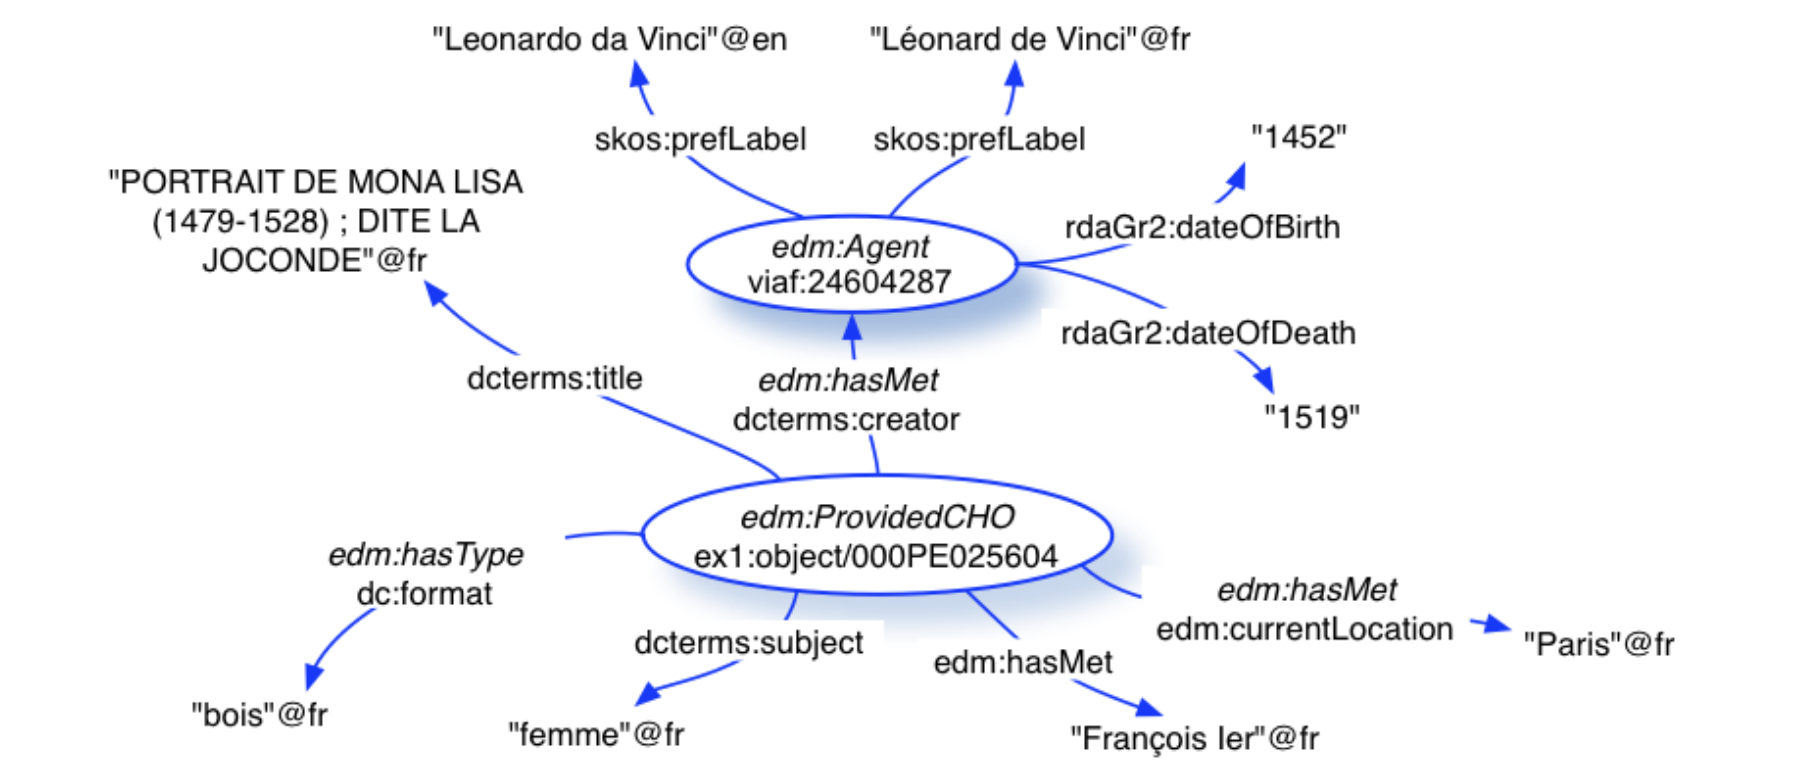
\includegraphics[width=15cm]{edm}
\caption{Extrait de \textit{Europeana Data Model Primer} ©Europeana.}
\end{figure}

Le web de données propose de nouvelles solutions, mais demeure une technologie avec certains défauts : il est très compliqué de faire face à un grand nombre de requêtes sur un corpus structuré selon le modèle RDF, et la création de liens entre les différents jeux de données est une pratique demandant beaucoup de temps pour son implémentation\footcite{rasmussen_pennington_connecting_2019}. Il faut plus que des données structurées en \gls{rdf} pour permettre un bon fonctionnement du web sémantique, la création de schémas de données de référence demeure un prérequis.
\begin{quotation}
[\textit{Traduction}]
Si chaque service web développe son propre schéma, cela équivaut à chaque ville et village développant leur propre borne d'incendie : il ne pourrait y avoir aucune collaboration entre les départements de pompiers, puisque les lances incendies ne fonctionneraient qu'avec leur borne locale. C'est seulement lorsque tous utiliseront les mêmes standards qu'une collaboration à grande échelle pourra être mise en place. \footnote{\textit{\inquote{If every web service developed its own schema for structuring its data, that would be the equivalent of every town and city developing its own type of fire hydrants : there could be no collaboration between fire departments because no department's hoses would fit any other department's hydrants. Only when everyone - or at least a significant portion of everyone - is using the same standards, is widespread collaboration possible}\cite[p.186]{pomerantz_metadata_2015}.}}
\end{quotation}

D'autres technologies travaillent à rendre interopérables les métadonnées des collections, à l'instar du protocole \gls{oai} ou des \gls{api}, qui permettent à des applications de communiquer entre elles\footcite{bermes_web_2013}. Les \gls{api}s sont des mécanismes très populaires pour accéder aux métadonnées sur les documents et aux documents eux-mêmes, elles sont dans la pratique presque davantage utilisées que les pages d'accueil des institutions\footcite{pomerantz_metadata_2015}. Les bibliothèques ont développé un standard très populaire spécifiquement dédié à l'interopérabilité des images, \gls{iiif}. Cette méthode de publication des données se base sur l'implémentation de différentes \gls{api}s et implique une structuration des métadonnées. Europeana a développé une extension de son modèle de métadonnées pour favoriser l'utilisation de \gls{iiif} par ses partenaires\footcite{iiif_consortium_home_nodate}.


%=====CONCLUSION TECHNIQUE

L'acquisition des compétences spécifiques pour les gestionnaires des collections numériques ne peut se limiter à la maîtrise d'une tâche, puisque la réussite du processus implique une vision d'ensemble et la prise de nombreuses décisions stratégiques (mise en place de standards de qualité pour la numérisation, définition des schémas de métadonnées, proposition d'un modèle, choix des outils pour favoriser l'interopérabilité etc.). \inquote{C'est tout une culture professionnelle du numérique qu'il faut élaborer et transmettre, de façon à permettre aux acteurs de s'inscrire dans un environnement global, de comprendre les implications de leurs choix et de leurs actions. \footcite[p.303]{claerr_manuel_2011}}. 

%=====ENJEU SUR LE CONTENU
\subsubsection{Enjeux sur le contenu}

Les collections numérisées sont disparates, proposant aux utilisateurs des ressources lacunaires ou contenant des doublons. Cela s'explique par des questions de financement, ou des questions de lois, de structures, de techniques\footcite{xie_discover_2016}\footcite{lopatin_library_2006}, mais également par le processus de sélection, du point de vue intellectuel, des ressources à numériser, et qui contribue à la problématique des silos. Les différentes stratégies de numérisation ont d'abord cohabité, développant pour chaque projet des critères propres, avant l'émergence des premières initiatives visant à les réunir. Bien que les critères de sélection intellectuels sont essentiels dans les entreprises de numérisation, ils n'ont jamais fait partie des contraintes de standardisation.\footcite{coutts_stepping_2017}.

Si les projets de numérisation de masse se sont construits dans la volonté de tout numériser et semblent à priori se passer de critères de sélection\footcite{lampert_ramping_2018}, la réalité est différente. Même si la sélection semble plus large, une prédominance des livres et des journaux dans les collections numérisées est à relever. De plus pour les \gls{agr}s que sont Europeana ou \textit{The Digital Public Library of America}, la sélection est fortement influencée par les collections et décisions des institutions partenaires, et par leurs positions géographiques. \footnote{La notion de \inquote{patrimoine européen} n'a pas attendu Europeana pour être diffusée à travers le monde. Le patrimoine des grandes bibliothèques américaines, numérisé par Google s'en est déjà chargé. C'est le patrimoine allemand, anglais, espagnol, français, italien de l'émigration européenne qui fonde les bases de celui des États-Unis. \cite{moatti_bibliotheque_2012}.} 

La vision de la bibliothèque universelle étant à priori issue du monde occidental et de la recherche, les plateformes d'accès aux produits de ces initiatives empêchent souvent leurs usages par des communautés ne partageant pas les mêmes normes\footcite{jones_public_2017}. Ce biais influence également la représentation des collections non occidentales dans les collections, qui suivent des formats de documents souvent mal pris en charge par les acteurs du marché\footcite{weiss_examining_2016}. 

Les projets de numérisation à plus petite échelle ne vont pas s'arrêter au profit des plus grands et l'intégration de ces collections signifie l'acceptation de leurs critères de sélection. \inquote{\textit{Digitisation work short of mass digitisation will continue, and selection criteria will be applied, whether in a structured or unstructured fashion\footcite[p.78]{coutts_stepping_2017}.}}

Le manque de normalisation pour la sélection peut sans doute être expliqué par le contexte et le développement rapide des projets de numérisation de masse, qui ont souvent \inquote{pallié au plus pressé} et se sont d'abord confrontés aux aspects techniques et légaux.

\begin{quotation}
[\textit{Traduction}] L'avancée de la numérisation a requis le développement et le renforcement de nombreux nouveaux éléments liés aux aspects techniques, structurels, légaux, financiers, au développement des interfaces de recherche. Ces aspects complexes évoluent de plus en plus rapidement, ce qui rend compréhensible le focus initial pour la création de standard et la coordination des pratiques associées. En conséquence, la mise en place de critères et d'aide à la sélection des ressources du point de vue de leurs contenus intellectuels a été négligé, alors même que ce champ d'étude était familier des acteurs de la culture et de l'information, habitués à les mettre en pratique dans la création de collections physiques.\footnote{\textit{\inquote{[...] the advent of digitisation required that many entirely new elements in the technical, infrastructural, discovery, preservation, legal and financial areas had to be developed, consolidated and matured. These were complex fields that changed rapidly. It is understandable that there was much emphasis on the creation of robusts standards and coordination of such practice; they were imperatives to apply the new technology effectively. As a consequence, guidance and criteria for the selection of content in terms of its intellectual value, a field that was already very familiar to information and heritage practitioners in relation to analogue materials, was somewhat overshadowed\cite[p.80]{coutts_stepping_2017}.}}}
\end{quotation}

Bien que les critères de sélection des objets à numériser se sont construits sans uniformisation, un groupe de critères communs émerge peu à peu. Margaret Coutts en propose huit, qui s'articulent en fonction du contexte des projets\footcite{coutts_stepping_2017}.
\begin{enumerate}
\item \textbf{L'accessibilité}

Les projets de numérisation se construisent autour de deux objectifs différents, celui de la préservation\footnote{Pour plus de détail, référez-vous à la section \ref{preservation}.}, et celui de l'accessibilité qui promet à la fois d'être élargie et enrichie par une publication en ligne. Ces deux notions font débat et dépendent fortement du contexte du projet.
\item \textbf{La notion de valeur}

Guidée par des critères intellectuels, historiques, physiques (format). Sélectionner en tenant compte de la valeur d'un document peut aussi être motivé par la notion de \inquote{valeur ajoutée}, découlant des nouveaux usages apportés par la version numérisée. La valeur est un choix subjectif qui dépend des intérêts des utilisateurs.

\item \textbf{La notion de rareté ou d'unicité}

Proposer pour la première fois la version numérisée. 

\item \textbf{La sélection thématique}

Une masse critique des documents numérisés est souvent atteinte par la mise en commun de plus petites entreprises, souvent articulées autour d'une thématique, d'un sujet particulier.

\item \textbf{Le format et le support}

Certains objets ont fait l'objet d'un numérisation plus rapide, à l'instar des livres, journaux, cartes et plans. 

\item \textbf{La cohérence}

Critère souvent utilisé lorsqu'il s'agit de mettre en commun différentes collections.

\item \textbf{La réunification virtuelle}

Permettant la réunification de ressources liées mais disséminées physiquement à travers différentes institutions.

\item \textbf{Le regroupement}

Propose un développement du critère précédent. Visant à réunir et enrichir des ressources déjà numérisées afin de développer de nouveaux services.

\end{enumerate}

Bernadette Dufrêne justifie la disparité des collections par leur développement initial autour de différents modèles, celui du musée où les pièces rares et trésors sont numérisés ; celui des archives où les documents sont numérisés selon une granularité d'ensembles thématiques liée à un fonds ; celui des bibliothèques, articulé souvent autour d'une charte documentaire détaillée visant à proposer la bibliothèque numérique idéale du chercheur et non élargir l'accès au patrimoine ; celui de Google, sans politique documentaire\footcite{dufrene_numerisation_2013}. Toutefois, l'absence de politique documentaire n'est pas forcément synonyme d'absence de critères de sélection comme nous l'avons vu plus haut.

Certains autres biais sont également listés, à l'instar des motivations des partenaires financiers qui peuvent venir imposer ou diriger certains choix, ou de la surreprésentation des collections des bibliothèques au détriment de celles des musées ou des archives, qui s'explique par un plus rapide développement de la numérisation dans ce secteur\footcite{coutts_stepping_2017}.

La croissance de la masse des données implique la mise en place de véritables directives dans la poursuite de la numérisation, afin de favoriser la réunification de ces données, d'éviter la redondance des collections et promouvoir la naissance de nouveaux usages\footnote{En Suède, un système de coordination a été mis en place par le bais de la Bibliothèque Nationale. \cite{dufrene_numerisation_2013}.}. 

 %===STOCKAGE
\subsection{Stockage sur le long-terme - préservation} \label{preservation}

Si la numérisation peut servir à préserver les objets physiques\footcite{xie_discover_2016}, la préservation signifie la maintenance sur le long-terme de l'accès aux objets numérisés ou à l'information contenue\footcite{coutts_stepping_2017}. Assurer cette longévité dépend de moyens techniques, économiques, légaux, organisationnels et structurels\footcite{xie_discover_2016}\footcite{georgetown_university_long_2009}. La prise en compte de cet enjeu est parfois laissée de côté dans les projets de numérisation de masse\footcite{lopatin_library_2006} alors que l'incertitude de pouvoir accéder sur la durée aux données a des impacts négatifs sur l'usage des plateformes et la conduite de projets de recherches dédiés\footcite{shankar_sustaining_2015}. 

Préserver implique souvent la copie de l'objet numérisé original, visant à la fois à servir de substitut et à proposer une version plus allégée pour les interfaces numériques\footcite{coutts_stepping_2017}. Les métadonnées de contexte sont importantes, puisque l'objet numérisé est souvent séparé de son format original dans le processus de numérisation\footcite{beaudoin_context_2012}.

Deux notions sont intrinsèques à la préservation, l'\inquote{intégrité} qui signifie que l'objet est le même que l'objet initialement numérisé, et l'\inquote{authenticité} qui consiste à s'assurer que l'objet est bien ce qu'il prétend être. La prise en compte de ces deux éléments doit assurer le long-terme de la compréhension et de l'usage de l'objet, alors même que les technologies seront modifiées\footcite{varniene-janssen_authenticity_2018}. 

En dehors de la question du stockage, on distingue trois technologies différentes pour la préservation des données\footcite{kowalczyk_digital_2018}. 
\begin{enumerate}
\item \textbf{La préservation des technologies de lecture}

Impliquant la conservation des anciens systèmes et des ordinateurs capables de les faire fonctionner.
\item \textbf{L'émulation}

Consiste à recréer un environnement technique capable d'exécuter les anciens programmes tout en fonctionnant avec une système moderne.

\item \textbf{La migration}

Passage d'un format de données vers un autre format. Souvent la méthode la moins coûteuse, mais implique certaines modifications de l'objet original, voir des pertes de données.

\end{enumerate}

Les technologies numériques présentent un paradoxe en terme de préservation. Ils multiplient les risques et les difficultés liés à la préservation sur le long-terme (dus à l'obsolescence des formats et programmes notamment) et proposent de nouvelles solutions et outils spécifiquement développés pour y pallier\footcite{xie_discover_2016}. 

Face aux difficultés posées par la préservation, de nouvelles pratiques voient le jour, visant à prendre en compte tous les aspects du cycle de vie des données (ajout de métadonnées standardisées, mise en place d'un plan de préservation, prise en compte des besoins des utilisateurs, valorisation et accessibilité) : la \gls{cur} de contenus numériques. Des infrastructures cross-institutions sont développées afin de partager les savoirs et les coûts\footcite{shankar_sustaining_2015}. Les bonnes pratiques développées pour le stockage des données ont conduits les dépôts institutionnels à devenir plus robustes, permettant à la fois l'ingestion de différents formats de données, leur organisation intuitive et proposant des fonctionnalités de recherche avancées\footnote{Le mouvement de l'\gls{os} a poussé les institutions a proposer des solutions efficaces pour les données de la recherche, qui peuvent être utilisées pour les projets de numérisation de masse. \cite{kowalczyk_digital_2018}.}. 

L'\gls{ue} a également financé des recherches visant à proposer des solutions de stockage sur le long-terme et des standards de métadonnées adaptés aux projets de numérisation de masse et leurs collections de données hétérogènes\footnote{Par exemple, le \textit{Scalable Preservation Environments} ou SCAPE projet, conclu en 2014.}\footcite{jurik_bridging_2015}.
\newpage
\subsection{Résumé des enjeux de la numérisation}
\begin{table}[H]
\centering
\begin{tabular}{|l|l|}
\hline
\rowcolor[HTML]{2E1A46} 
{\color[HTML]{FFFFFF} \textbf{Enjeux}}                                                                                   & {\color[HTML]{FFFFFF} \textbf{Résumé}}                                                                                                                                                                                                                                                                                                                                                                                                                                                                                                                                                                                                                                                                                                                                                                    \\ \hline
{\color[HTML]{2E1A46} \textbf{\begin{tabular}[c]{@{}l@{}}Amener différents\\ acteurs à collaborer\end{tabular}}}         & \begin{tabular}[c]{@{}l@{}}Susceptible d'impacter tous les autres enjeux, une collaboration \\ de qualité doit être mise en place entre les différents partenaires.\end{tabular}                                                                                                                                                                                                                                                                                                                                                                                                                                                                                                                                                                                                                          \\ \hline
{\color[HTML]{2E1A46} \textbf{\begin{tabular}[c]{@{}l@{}}Financement et \\ partenariats \\ public-privé\end{tabular}}} & \begin{tabular}[c]{@{}l@{}}Les coûts élevés impliquent des fonds privés. Ces partenariats \\ suscitent des craintes et manquent d'encadrement. Peu d'argent \\ est dédié à la préservation sur le long-terme.\end{tabular}                                                                                                                                                                                                                                                                                                                                                                                                                                                                                                                                                                                \\ \hline
{\color[HTML]{2E1A46} \textbf{Droit d'auteur}}                                                                           & \begin{tabular}[c]{@{}l@{}}Projets souvent limités aux \oe{}uvres libres de droit. Cela coûte cher\\ de rechercher les détenteurs de droits. Les \oe{}uvres du 20\up{e} siècle \\ sont sous-représentées. Pas de cadre légal européen, mais de \\ nombreux régimes nationaux. Réflexions autour de la directive sur \\ les \oe{}uvres orphelines et la prise de risques.\end{tabular}                                                                                                                                                                                                                                                                                                                                                                                                                                                          \\ \hline
{\color[HTML]{2E1A46} \textbf{\begin{tabular}[c]{@{}l@{}}Sortir des silos : \\ enjeux techniques\end{tabular}}}          & {\color[HTML]{333333} \begin{tabular}[c]{@{}l@{}}L'objectif est de rassembler des collections de provenances \\ différentes et permettre leurs interrogations en-dehors du silo de\\ leurs institutions.\\ Nécessité de fixer des standards pour la numérisation, et de définir \\ des critères de qualité.\\ Nécessité de fixer des standards pour les métadonnées, \\ présentation des différentes typologies, du rôle du schéma et de la\\ place des vocabulaires contrôlés.\\ Présentation des quatre principes du web sémantique et usages du \\ RDF, introduction d'autres outils favorisant l'interopérabilité \\ (OAI-PMH, APIs, IIIF).\\ Face à ces enjeux techniques en constante évolution, il est \\ nécessaire de développer la formation des gestionnaires de \\ collections.\end{tabular}} \\ \hline
{\color[HTML]{2E1A46} \textbf{\begin{tabular}[c]{@{}l@{}}Sortir des silos : \\ enjeux sur le \\ contenu\end{tabular}}}   & \begin{tabular}[c]{@{}l@{}}Un processus de sélection intellectuel non coordonné, qui \\ contribue à la création de collections disparates et redondantes\\ et ne favorise pas la mise en commun des collections. Nécessité\\ de mettre en place des directives et de prendre conscience des \\ typologies derrière ces critères de sélection (valeur, format, \\ unicité, accessibilité, thématique, cohérence, réunification \\ virtuelle, regroupement).\end{tabular}                                                                                                                                                                                                                                                                                                                                   \\ \hline
{\color[HTML]{2E1A46} \textbf{\begin{tabular}[c]{@{}l@{}}Stockage sur le \\ long-terme - \\ préservation\end{tabular}}}  & \begin{tabular}[c]{@{}l@{}}Préserver l'accessibilité sur le long-terme des données \\ numérisées afin d'en favoriser l'usage. Différentes méthodes \\ (émulation, préservation des technologies, migration) et systèmes\\ permettent la mise en place de cette préservation. Le coût reste\\ élevé, et les projets sont souvent construits sans plan de \\ préservation.\end{tabular}                                                                                                                                                                                                                                                                                                                                                                                                                     \\ \hline
\end{tabular}
\caption{Résumé des enjeux de la numérisation}
\end{table}   
\newpage

%====================CHAPITRE 3 (keyword context)
\chapter{Contexte du projet Time Machine}

Pour comprendre l'articulation du projet Time Machine au sein de l'histoire des projets de numérisation de masse et les réponses apportées aux enjeux liés à l'envergure de ces initiatives, il nous faut premièrement introduire le contexte du projet. Nous tenterons de définir dans le troisième temps de ce mémoire, si ses objectifs et solutions l'inscrivent dans une démarche de continuité ou contribuent à positionner les entreprises de numérisation de masse en tant que nouvel acteur de l'information. 

Cette présentation du cadre décrit d'abord le contexte académique de l'\gls{epfl} et de la recherche en humanités numériques qui l'ont vu naître, puis le projet \textit{Venice Time Machine} et les diverses activités du \gls{dhlab}, racines des développements futurs.

Nous terminons ce chapitre par une présentation de Time Machine, ses objectifs et  son organisation au moment de commencer notre stage.

Nous décrirons plus précisément notre mission de stagiaire et la réponse apportée par Time Machine aux enjeux de la numérisation dans la troisième partie de ce mémoire.

\section{La recherche en humanités numériques} 
%(keyword digitalhumanities)
\inquote{Nouveau} domaine d'étude, dont l'appellation est apparue au tournant des années 2000, les \textit{digital humanities (DH)}, humanités digitales ou humanités numériques pour les chercheurs francophones \footnote{Nous privilégions l'emploi du terme humanités numériques dans ce mémoire, qui est l'appellation utilisée en France, lieu de notre soutenance.}, proposent des programmes de recherche en cooccurrence avec les technologies informatiques et les différentes disciplines des sciences humaines.\footnote{\cite[p. 2]{meunier_paradoxe_2019}} Si les tentatives de définition abondent et demeurent volontairement larges, c'est aussi par refus d'établir \og une définition qui préexisterait à l'usage\fg{}\footnote{\cite[p. 2]{caraco_les_2012}}. 

Notre stage se déroulant au sein d'un laboratoire d'humanités numériques, il nous semble pertinent d'introduire quelques fondamentaux du domaine, pour mieux comprendre les origines académiques du projet Time Machine. Les débats étant à ce jour vifs parmi les communautés de chercheurs, dont les historiens, \og les réunions DH créent de nouveaux temps d'échange qui dépassent les thématiques et les périodes historiques, pour mettre en dialogue antiquisants, médiévistes, modernistes et contemporanéistes\fg{}\footnote{\cite[p. 5]{clavert_les_2019}}, nous ne prétendrons pas être exhaustif. 

Les humanités numériques constituent des zones d'échange, de projets à la frontière entre plusieurs disciplines, créant dans leurs pratiques de nouveaux espaces d'expression et leurs organisations associées, à l'instar d'Humanistica :  \textit{Association francophone des humanités numériques}, \footnote{\cite{association_francophone_des_humanites_numeriques_humanistica_nodate}} des conférences \gls{dh} Benelux \textit{\og an initiative that aims to further the collaboration between Digital Humanities activities in Belgium, The Netherlands, and Luxembourg \fg}{}\footnote{\cite{dhbenelux_2019_dhbenelux_nodate}}, des THATCamp \textit{\og The Humanities and Technology Camp \fg}{}\footnote{\cite{thatcamp_humanities_nodate}}, de Dariah en Europe \textit{\inquote{a pan-european infrastructure for arts and humanities scholars working with computational methods}}\footnote{\cite{dariah_digital_nodate}}, ou encore des conférence DH organisées par l'\textit{\og Alliance of Digital Humanities Organizations\fg}{}\footnote{\cite{alliance_of_digital_humanities_organizations_about_nodate}}.

La variété des approches est grande et diffère en fonction des rôles spécifiques attribués à l'expert des humanités ou à l'expert de l'informatique. Dans le premier type d'approche, les humanités numériques sont la suite des études menées en humanités, le numérique étant alors un outil aux services de \textit{\inquote{what is important today is not that we are doing work with computers, but rather that we are doing the work of the humanities, in digital form.}}\footnote{\cite[p.17]{schreibman_new_2016}}. Dans le deuxième type d'approche, l'informaticien est expert, et les données une fois générées sont offertes aux interprétations des chercheurs en humanités \footnote{\cite{meunier_paradoxe_2019}}. Cette situation a été identifiée par Jean-Guy Meunier comme le paradoxe des humanités numériques, lorsque les experts techniques estiment que \inquote{les traitement interprétatifs manquent de rigueur et de scientificité}\footnote{\cite[p.6]{meunier_paradoxe_2019}} et que les experts en humanités considèrent toute formalisation comme trop réductrice et peu capable de \inquote{rendre compte adéquatement de la complexité des objets traités} \footnote{\cite[p.6]{meunier_paradoxe_2019}}. La recherche en humanités numériques est dès lors une démarche complexifiée par les questions de compréhension et d'interprétation posées par ses objets d'étude, \inquote{d’autant qu’il n’y a pas une, mais des communautés \gls{dh}, qui distinguent notamment des approches anglo-saxonnes et européennes}\footnote{\cite[p.41]{clavert_les_2019}}. Pour le Professeur Willard McCarthy \footnote{Professeur au sein du département des humanités numériques du King's College de Londres.}, ce n'est pas uniquement le champ qui doit être interdisciplinaire, mais les personnes qui le pratiquent qui devraient tendre à l'être, se tenir informées de ce qui se fait ailleurs pour enrichir leurs expériences de recherche\footnote{\cite{schreibman_new_2016}}. Certains experts proposent une cartographie des champs de recherche : 

\begin{quotation}La variété des approches en \gls{dh} peut répondre à des interrogations en termes à la fois de recueils et gestion des sources de données, d'analyse et de représentation via des outils numériques - comme l'usage ou la constitution de bases de données, de cartographie de liens, d'étude sémantique ou lexicale etc. - ou encore de valorisation, notamment dans le cadre de l'histoire numérique publique.\footnote{\cite[p.35-36]{clavert_les_2019}}\end{quotation}

Si les démarches en humanités numériques sont multiformes et se distinguent de \inquote{tout un champ d'expérimentation croisant SHS et informatique (\textit{literary / linguistic / humanities computing}}\footnote{\cite{mounier_lou_nodate}}, les ancêtres de la discipline semblent communément acceptés, à l'instar du père Roberto Busa, jésuite pionnier de la numérisation et de l'analyse de corpus et de Franco Moretti, auteur de \textit{Graphes, cartes et arbres. Modèles abstraits pour une autre histoire de la littérature, 2008}, qui reste une référence pour son concept de lecture distante.\footnote{\cite{gefen_humanites_2017}} La \textit{Text Encoding Initiative (TEI)}, créée en 1987, figure aussi en bonne position puisqu'elle place les données au centre de son étude et s'adapte aux évolutions des outils informatiques.\footnote{\cite{clavert_les_2019}}. D'autres précurseurs communs aux projets de numérisation de masse pourraient figurer dans ce palmarès, notamment Paul Otlet, et Ted Nelson l'inventeur de la notion d'hypertexte.\footnote{\cite{clavert_les_2019}} Les projets en humanités numériques s'offrent à la fois comme outil et objet d'étude, tant leurs histoires s'écrivent au présent. 

\begin{quotation} [...] les humanités numériques ont permis l'émergence d’un vaste et riche patrimoine numérique, sources primaires de leur propre histoire que les historiens pourront très clairement exploiter, par l’hybridation de leurs outils maîtrisés de longue date (la lecture proche) avec ceux des \textit{digital humanities}, au premier rang desquels la lecture distante jouera un grand rôle.\footnote{\cite[p.43]{clavert_les_2019}}\end{quotation}

Time Machine fait de la question de la \gls{num} de masse l'un de ces enjeux. C\oe{}ur de nombreux projets en humanités numériques, l'acte de numérisation articule plusieurs moments (choix de la collection, conversion des documents papiers en versions électroniques, traduction du format électronique en format binaire, reconstruction de la structure du document, identification des caractères etc.)\footnote{\cite{meunier_paradoxe_2019}} et dans une même entreprise voient se confronter les différents rôles attribués à l'expert des humanités ou à l'expert de l'informatique. 

\begin{quotation}Ainsi, pour un expert des humanités, la constitution d’un corpus apparaîtra avant tout comme une activité de type herméneutique et l’ordinateur ne sera qu’un assistant, à l’inverse pour un expert de l’informatique, la numérisation apparaîtra avant tout comme l’application de technologies computationnelles d’une grande complexité.\footnote{\cite[p. 29]{meunier_paradoxe_2019}}\end{quotation}

Tout en s'inscrivant dans les démarches historiques des humanités numériques, Time Machine semble incarner les différents paradoxes de cette pensée académique au sein d'un même projet et promet de devenir à son tour objet d'étude de cette histoire.

\begin{quotation}Ainsi, au contact des humanités numériques, les historiens sont amenés à revisiter plusieurs aspects de la fabrique d’une histoire qui aujourd’hui articule productions individuelles et collectives, sous l’effet certes du numérique, mais aussi d’une culture du projet, qui innerve toutes les disciplines [...].\footnote{\cite[p. 42-43]{clavert_les_2019}}\end{quotation}

%-------------------------------------------------------------------------- keyword context
\section{Le Laboratoire d'humanités numériques de l'EPFL}
L'\gls{epfl} ouvre ses portes en 1853 sous le nom de l'École Spéciale de Lausanne. Au fil des années, l'école grandit, voyant de nouvelles spécialisations s'intégrer à son cursus (électricité, physique, architecture etc.), et d'une académie, devient université. Elle prend son nom actuel en 1969, année qui coïncide avec le début de son établissement sur le campus d'Écublens-Dorigny (Suisse). Réputés sélectifs, les cursus ne désemplissent pas et l'offre continue de croître. Dès 1991, la construction d'un parc scientifique hébergeant une dizaine de compagnies favorise le développement des activités de recherche. En 2003, année de son 150\up{ème} anniversaire, l'école compte plus de 6000 étudiants. 2014 marque la création de deux nouveaux campus en Suisse avec l'ouverture de l'\gls{epfl} Valais\footnote{\cite{epfl_epfl_nodate-1}} (dix laboratoires actifs dans les domaines de l'énergie, de l'environnement et de la santé) et de l'\gls{epfl} Fribourg\footnote{\cite{epfl_epfl_nodate}} (\textit{\og smart living lab \fg{}}  dédié aux recherches en technologies de la construction, bien-être et comportements, interaction et processus de conception, et systèmes énergétiques). En 2015, le nombre d'étudiants franchit la barre des 10'000\footnote{\cite {epfl_history_nodate}}.

En 2019, l'\gls{epfl} compte cinq facultés, trois collèges, plus de 11'000 étudiants, et quelques 210 compagnies constituent son parc scientifique\footnote{\cite {epfl_innovation_nodate}}. Son rayonnement s'étend à l'international, l'\gls{epfl} est en bonne position dans les classements universitaires européens et mondiaux.

Fondé en 2002, le Collège des Humanités (CDH) est un  un \og lieu de convergence des sciences humaines et sociales au coeur de l'\gls{epfl}, basé sur le concept de \gls{poly}, reflétant la nécessité pour les futurs ingénieurs et scientifiques d'adopter une perspective pluraliste face aux enjeux auxquels ils sont confrontés\fg{}\footnote{\cite {epfl_vision_nodate}}. Les perspectives s'organisent autour de quatre grandes thématiques : l'interdisciplinarité, la conscience globale (comprendre l'histoire des technologies pour mieux les faire évoluer), la citoyenneté et la créativité (engagement à travers l'art et la production artistique). La recherche au sein du CDH se compose de deux instituts, le \textit{Digital Humanities Institute (DHI)} et l'\textit{Institute for Area and Global Studies (IAGS)}, et d'un pôle soutenant des projets transdisciplinaires entre l'Université de Lausanne (UNIL) et l'\gls{epfl} : le \textit{Collaborative Research on Science and Society (CROSS)}\footnote{\cite {epfl_cross_nodate}}. Le CDH coordonne également le programme d'enseignement en sciences humaines et sociales pour tous les étudiants de l'\gls{epfl} et le DHI propose un master en humanités digitales et est lié au programme doctoral en humanités digitales \footnote{\cite {noauthor_formations_nodate}}.

Le \gls{dhlab} dans lequel nous avons effectué notre stage, constitue l'un des trois laboratoires du DHI, aux côtés du \textit{Digital and Cognitive Musicology Laboratory (DCML)} et du \textit{Laboratory for Experimental Museology (eM+)} et de plusieurs groupes thématiques de recherche (\textit{Social Computing Group},\textit{ Social Media}).\footnote{\cite {epfl.dhlab_dh_nodate}} 

Le \gls{dhlab} est fondé en 2012 par le Professeur Frédéric Kaplan avec pour objectif de développer de nouvelles approches informatiques pour l'étude du passé et la découverte du futur. Le Professeur Kaplan est également le créateur du Master en humanités digitales du DHI et co-organisateur de la \textit{Digital Humanities 2014}, conférence internationale de l'\textit{Alliance of Digital Humanities Organizations (ADHO)}\footnote{\cite {epfl.dhlab_dh_2019}} à Lausanne, qui demeure l'un des plus grands rassemblements scientifiques du domaine. 

\begin{figure}[H]% force à placer l'image au sein de notre balise figure
\centering
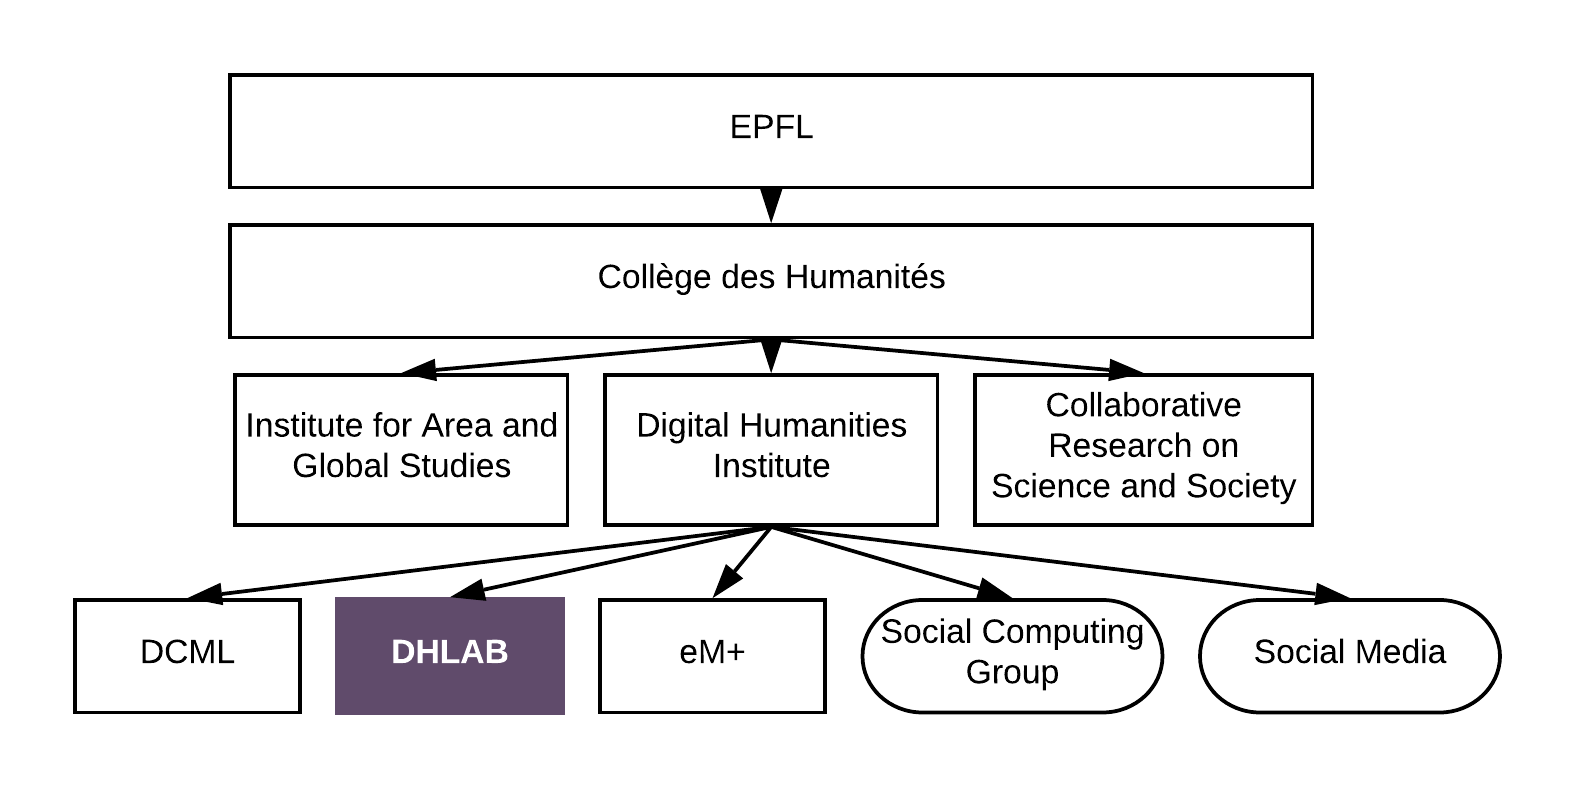
\includegraphics[width=15cm]{dhlab.png}
\caption{Le \gls{dhlab} au sein de l'\gls{epfl}}
\end{figure}

\section{Venice Time Machine}
Né de la crainte de voir les informations non digitales tomber dans \inquote{les oubliettes de l'histoire}\footnote{\cite{dubuc_venice_2017}}, initié en 2012 par l'\gls{epfl} et l'université Ca'Foscari de Venise, le projet vise à construire un modèle multidimensionnel de Venise et de ses évolutions, sur une période de 1000 ans : une machine à remonter le temps. Conscients dès le départ que les enjeux du projets nécessitent bien plus que de la puissance de calcul informatique, les initiateurs s'allient le secours d'historiens et d'archivistes pour mettre en place les processus de \gls{num}\footnote{\cite{abbott_time_2017}}. La transformation des 80 kilomètres d'archives vénitiennes en un système d'informations nécessite en plus un grand travail d'indexation et de cartographie pour aboutir à ce qui se veut une version augmentée de \textit{Google Maps}, offrant en plus un ancrage temporel\footnote{\cite{world.minds_frederic_nodate}} : un croisement entre histoire et \textit{\gls{bigd}}\footnote{\cite{rts_remonter_nodate}}. 

Les archives numérisées par le projet proviennent de deux sources différentes\footnote{\cite{evangelista_time_2018}} : 
\begin{itemize}
\item \textbf{Les Archives d'Etat de Venise} : en 2018, 190'000 documents avaient été numérisés
\item \textbf{La Fondation Cini} : la Fondation possède un million de photos d'art, en 2018 quelques 720'000 documents photographiques avaient été numérisés
\end{itemize}
Face à d'immenses corpus souvent manuscrits, les outils permettant la lecture automatique sont cruciaux. L'EPFL rejoint le projet européen \textit{Recognition and Enrichment of Archival Documents (READ)}\footnote{\cite{noauthor_recognition_nodate}} poursuivant des objectifs similaires, et emploie une partie de ses équipes à développer des solutions d'\gls{appauto}\footnote{\cite{nature_video_virtual_nodate}}. 

Avec le projet vénitien, l'\gls{epfl} souhaite développer, tester et démontrer l'efficacité d'une méthode appelée à se déployer avec Time Machine à travers l'\gls{ue}\footnote{\cite{arte_venice_nodate}}. Sans le succès du Venise Time Machine, il n'y a pas de Time Machine\footnote{\cite{kaplan_cartographie_2018}}. 

\subsection{Développements technologiques}
Le projet se poursuivant actuellement, de nombreux outils, techniques, méthodologies ont été spécialement dédiés à son avènement. En plus de la \gls{num}, il a fallu apprendre aux ordinateurs à automatiquement extraire certains types d'information, ce qui a impliqué un grand travail d'indexation manuelle. Tous ces éléments viendront enrichir la future interface de Time Machine et contribueront à la création de ce \textit{\gls{bigd}} du passé. L'envergure de ce projet étant trop vaste pour en lister tous les composants, voici un aperçu de leurs variétés :

\begin{itemize}
\item \textbf{The Replica Scanner} : numériser massivement a induit à  la création de divers scanners. Celui-ci, développé avec Adam Lowe de Factum Arte\footnote{\cite{s.l_factum_nodate}} est capable de numériser un document photographique recto verso toutes les quatre secondes.
\item \textbf{DhCanvas} : moteur de recherche associé aux documents numérisés, permettant la recherche dans le document original et son contenu,  fonctionnant comme un outil participatif de transcription. Les utilisateurs autorisés peuvent corriger les erreurs d'extraction\footnote{\cite{evangelista_time_2018}}.
\item \textbf{Replica} : une interface de recherche spécialement dédiée aux fonds des images numérisées de la Fondation Cini, proposant une recherche visuelle (par motifs, position des personnages etc.) et textuelle des documents et permettant d'établir des connections entre des images\footnote{\cite{evangelista_time_2018}}.
\item \textbf{Venice Scholar} : travail consacré aux ouvrages et journaux scientifiques vénitiens numérisés et dont les citations ont été automatiquement extraites, pour pouvoir étudier l'historiographie vénitienne\footnote{\cite{evangelista_time_2018}}.
\item \textbf{DhSegment} : confronté à l'enjeu de traiter l'immense masse des images numérisées, ce système se base sur les \gls{reneu} pour en extraire automatiquement certaines parties (lignes, encadrés, zone de texte etc.)\footnote{\cite{epfl.dhlab_introduction_nodate}}.
\end{itemize}

\begin{figure}[H]% force à placer l'image au sein de notre balise figure
\centering
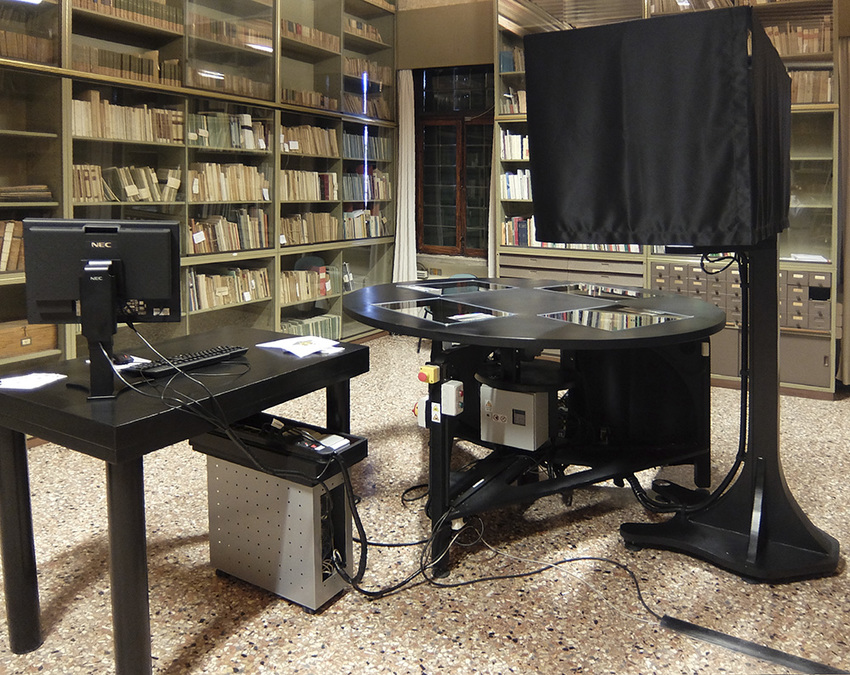
\includegraphics[width=15cm]{replica_scanner.jpg}
\caption{Le scanner Replica à la Fondation Cini, \textit{© Copyright 2019 Factum Foundation}}
\end{figure}

\section{Le projet Time Machine}

Le 14 décembre 2016, Frédéric Kaplan, Professeur et occupant de la chaire d'humanités digitales de l'\gls{epfl}, publie dans le journal suisse \textit{Le Temps}, le \href{https://www.letemps.ch/opinions/leurope-construire-premiere-time-machine}{manifeste} du projet Time Machine. L'intérêt du public et des institutions patrimoniales pour le projet Time Machine s'éveille et l'aventure est officiellement lancée ; Time Machine peut se lancer à la conquête de l'Europe et créer sa \inquote{machine à remonter le temps}. 

\begin{quotation}
L’Europe a inventé le web. Le web est devenu la matrice d’un monde nouveau. Les acteurs qui, les premiers, en comprirent la logique, dominent aujourd’hui notre monde. Une trentaine d’années plus tard, le virage spatio-temporel de l’Internet, en plongeant l’information numérique dans un espace bien plus large, redéfinit les règles du jeu.

Le projet Time Machine peut donner à l’Europe la technologie de son renouveau: une occasion unique pour construire notre futur à partir de notre patrimoine commun, une occasion unique pour nous retrouver\footnote{\cite{noauthor_leurope_2016}}.
\end {quotation}

\begin{figure}[H]% force à placer l'image au sein de notre balise figure
\centering

\includegraphics[width=15cm]{TM_logo.png}
\caption{Time Machine, logo \textit{© Copyright 2019 Time Machine}}
\end{figure}

\subsection{FET Flagships ou la recherche de financement}\label{fet}
A travers l'initiative des \textit{FET Flagships} ou \inquote{Initiatives-phare des technologies Futures et Emergentes}, la Commission européenne mettait au concours un soutien financier d'un milliard d'euros réparti sur dix ans. Les projets éligibles se devaient d'être visionnaires, de proposer des solutions scientifiques et technologiques innovantes et de réunir sur le long-terme autour d'un objectif commun et d'une feuille de route aux solutions ambitieuses, des équipes de recherche interdisciplinaires\footnote{L'\gls{epfl} pilote déjà un projet doté d'un tel financement, le \inquote{Human Brain Project}.}\footnote{\cite{moriscl_fet_2013}}. 

L'ambition de Time Machine s'accordant avec les objectifs fixés par la Commission, ses initiateurs (\textit{l'\gls{epfl} s'est alliée le concours de 32 partenaires pour développer et financer la proposition du projet, dont l'École Nationale des Chartes}) se sont lancés dans la course. L'histoire ne s'est pas faite sans embûches, Time Machine s'inscrivant sous le sigle de la culture, il fallut d'abord faire modifier les critères de sélection définis par l'\gls{ue} qui s'opposaient aux candidatures issues du milieu \footnote{\cite{rts_invite_nodate}}. En 2016, Time Machine est officiellement retenu comme candidat et en février 2019, le projet est classé premier parmi les six finalistes en lice pour la dernière ligne droite, avec cette fois une enveloppe d'un million d'euros et une année (à compter du 1er mars 2019) pour démontrer de l'organisation et de la faisabilité du projet.

Cette première victoire est nuancée, puisque coïncidant avec une année de votation, le programme de recherche européen \textit{Horizon Europe}, doté d'une enveloppe de quelque cent milliards d'euros pour la période 2021-2027, peine à se stabiliser \footnote{\cite{noauthor_crise_nodate}}. Le projet des FET Flagships est abandonné par la Commission européenne sans que pour l'heure une solution concrète ait été proposée aux six projets concurrents \footnote{\cite{rts_coup_2019}}. 

Nous avons commencé notre stage en cette période d'incertitude financière, étant à la fois contraints par l'\gls{ue} de planifier la mise en route du projet puisque le million a été perçu, mais sans certitude quant à l'ampleur finale du budget alloué.

\subsection{Time Machine, quels objectifs ?}

Dès 2014, le Professeur Frédéric Kaplan propose un modèle en forme de \inquote{champignon} pour expliciter l'ampleur des informations dont l'humain dispose pour évaluer une période donnée\footnote{\cite{ted_frederic_nodate}}. L'image est porteuse, plus l'on se rapproche du présent, plus le cône s'élargit. Face à une société désormais digitale, le risque est grand de perdre pour toujours l'accès aux informations contenues uniquement sous formes physiques, les enjeux liés à la conservation de ces documents sont réels, mais comment parvenir à rétablir un équilibre entre l'information du passé et l'information du présent\footnote{La \textit{factsheet} du projet, donnée en annexe \ref{factsheet}, offre une synthèse plus visuelle.} ? 

\begin{figure}[H]% force à placer l'image au sein de notre balise figure
\centering
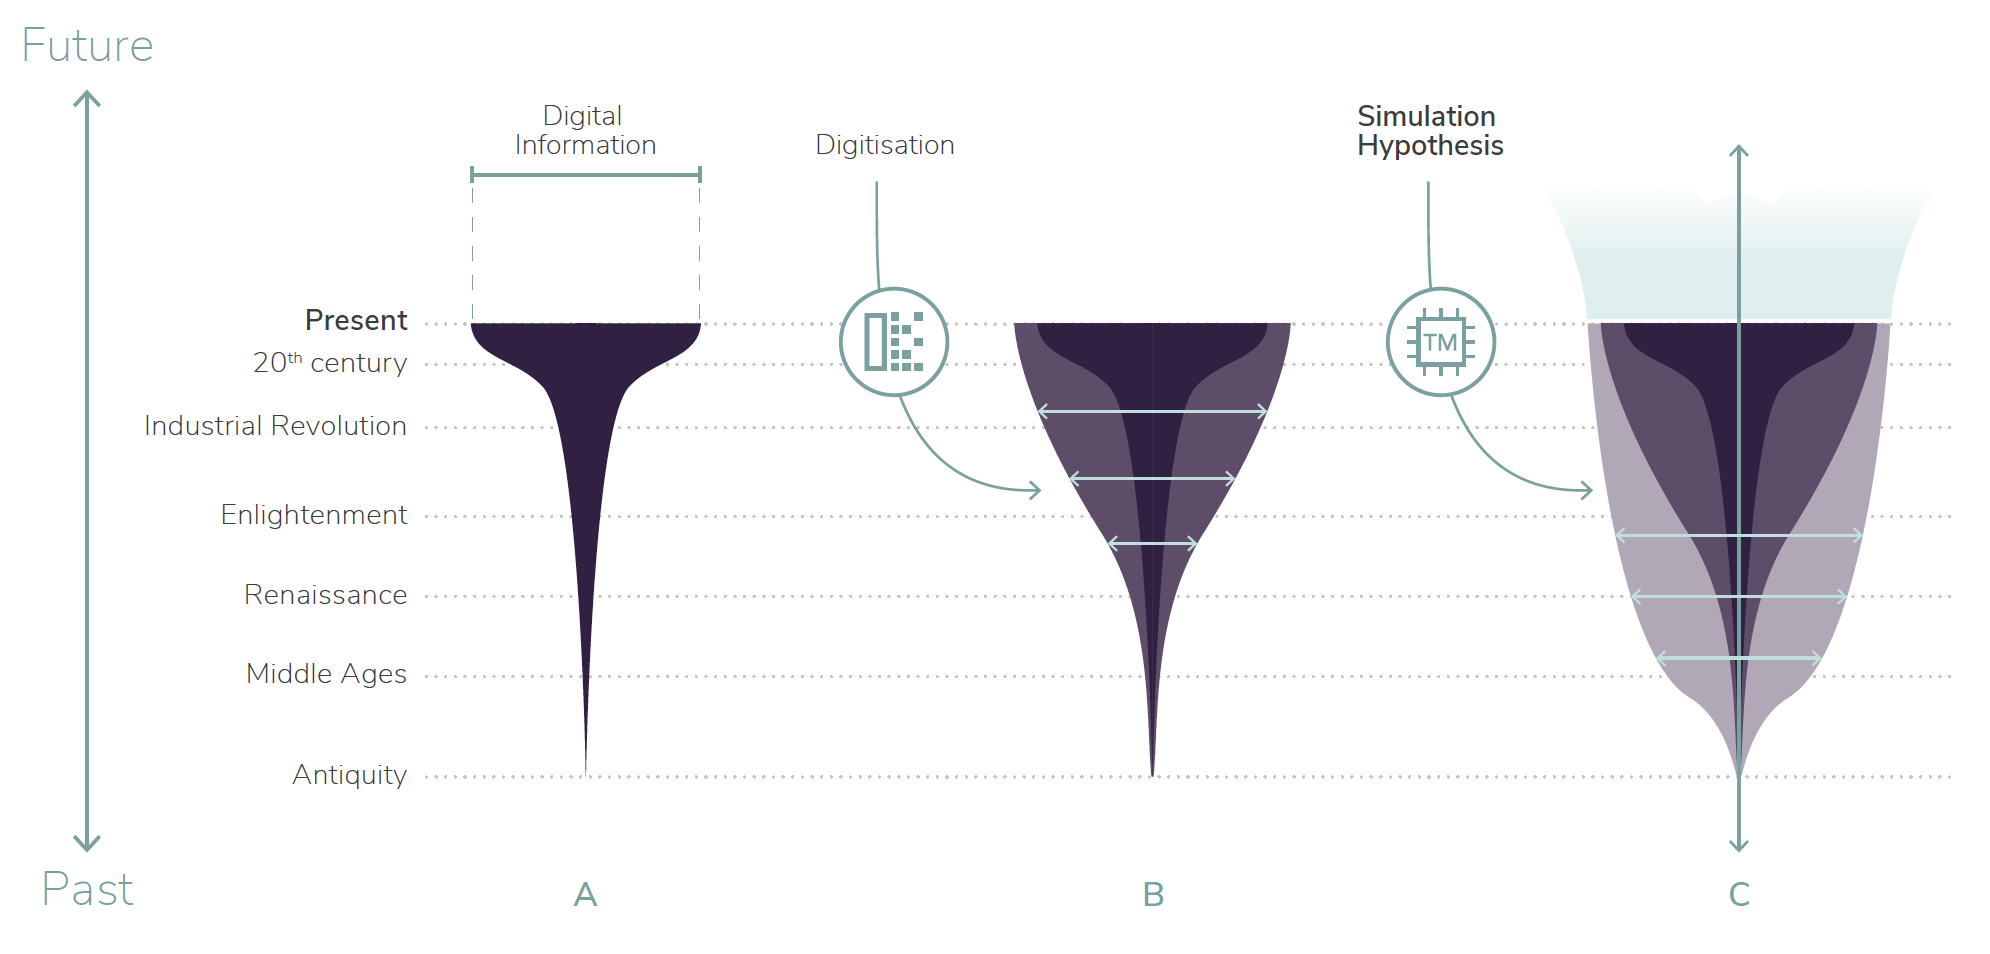
\includegraphics[width=17cm]{champ_info.png}
\caption{Time Machine, Information's Mushroom \textit{© Copyright 2019 Time Machine}}
\end{figure}

En visant comme résultat la création d'un \gls{graph} de données du passé, le \textit{\gls{bigd} of the past}, impliquant le développement de processus, technologies et innovations nécessaires à sa réalisation, Time Machine poursuit différents objectifs\footnote{Time Machine Manifesto, 2019 URL : https://documents.icar-us.eu/documents/2019/05/time-machine-manifesto.pdf} :

\begin{itemize}
\item Révolutionner les connaissances en \gls{ia} et dans le domaine des sciences de l'information et de la communication, positionnant l'Europe comme meneur sur le marché de l'extraction et de l'analyse d'énormes jeux de données hétérogènes et complexes, induits par les activités et réalisation passées et présentes du genre humain.
\item Offrir de nouvelles perspectives aux chercheurs en humanités et sciences sociales, leur permettant de positionner leurs objets d'étude à l'échelle plus large de l'histoire et de la culture européenne.
\item Devenir moteur et acteur de l'\textit{\gls{os}} et mettre à disposition les données du projet dans des dépôts ouverts et publics.
\item Offrir un flux de connaissances à l'enseignement, encourageant les réflexions sur le long-terme et l'apprentissage de la pensée critique.
\item Devenir un nouvel acteur économique, par la création d'emplois, services et produits appelés à influencer les secteurs clés de l'économie européenne.
\end{itemize}

\subsection{Quelle(s) méthode(s) pour Time Machine ?}

Créer un système d'information d'ampleur européenne basé sur un \gls{graph} de données du passé implique le déroulement de plusieurs étapes\footnote{\cite{ted_frederic_nodate}}\footnote{\cite{kaplan_cartographie_2018}} et le déploiement de technologies nécessaires à leurs succès. Se basant sur les innovations et méthodologies du projet vénitien, des projets menés en parallèle par l'équipe du \gls{dhlab}, et de ceux conduits par les partenaires du futur réseau, Time Machine entend mener ses révolutions technologiques à différents niveaux\footnote{Les partenaires étant actuellement plus de 300, il est impossible de rendre justice dans le cadre de ce travail à la multitude des projets en cours appelés à contribuer à la mise au point de Time Machine.} : 

\begin{enumerate}
%==========Première technologie ==================
\item \textbf{Numérisation massive des documents - archives - patrimoine bâti} 

Poursuivre le développement des outils de numérisation pour les documents (2D) et bâtiments (3D). 

Depuis 2018, l'\gls{epfl} conjointement avec la fondation Cini et Factum Arte\footnote{\cite{s.l_factum_nodate}} a créé un centre d'expérimentation et de formation aux techniques de numérisation à Venise : \textit{ARCHiVe, Analysis and Recording of Cultural Heritage in Venice}\footnote{\cite{noauthor_archive_nodate}}, diverses études sont en cours pour créer des scanners de nouvelles générations, mais également des programmes facilitant le suivi et l'automatisation des processus (traitement automatique de la post-production, ajout de métadonnées, indexation du texte). Les technologies d'\gls{appauto} sont utilisées par souci d'automatisation et de gain de temps. 

Les innovations apportées par ce \inquote{modèle} vénitien seront amenées par Time Machine, avec l'aide des acteurs locaux du marché de la numérisation, à se répandre et se développer à travers l'Europe, créant un réseau Time Machine de centres de numérisation européen. Cette uniformisation des processus permettra l'harmonisation des coûts et la garantie de la qualité des données. 

Une fois les données numérisées, leur stockage doit être assurés en vue de leur valorisation. Si un grand nombre d'institutions patrimoniales disposent de leurs propres serveurs, ce n'est pas forcément le cas des plus petites et ce n'était pas celui des archives vénitiennes. Une \textit{Time Machine Box}\footnote{\cite{epfl.dhlab_home_nodate}} a été développée, visant à accompagner les partenaires dans leurs démarches de numérisation et leur offrir une alternative de stockage en local.

La numérisation du patrimoine bâti implique l'utilisation des techniques de la \gls{photo} et l'alignement de différents nuages de points. L'ambition de Time Machine étant à l'échelle de villes, les technologies actuelles devront être améliorées. Le projet \textit{ScanVan (2016-2020)}, conduit par le \gls{dhlab}, a pour objectif le développement d'un véhicule capable de numériser les villes et de créer automatiquement des modèles 3D de ces territoires\footnote{\cite{epfl.dhlab_2016_nodate}}. 
\begin{figure}[H]% force à placer l'image au sein de notre balise figure
\centering
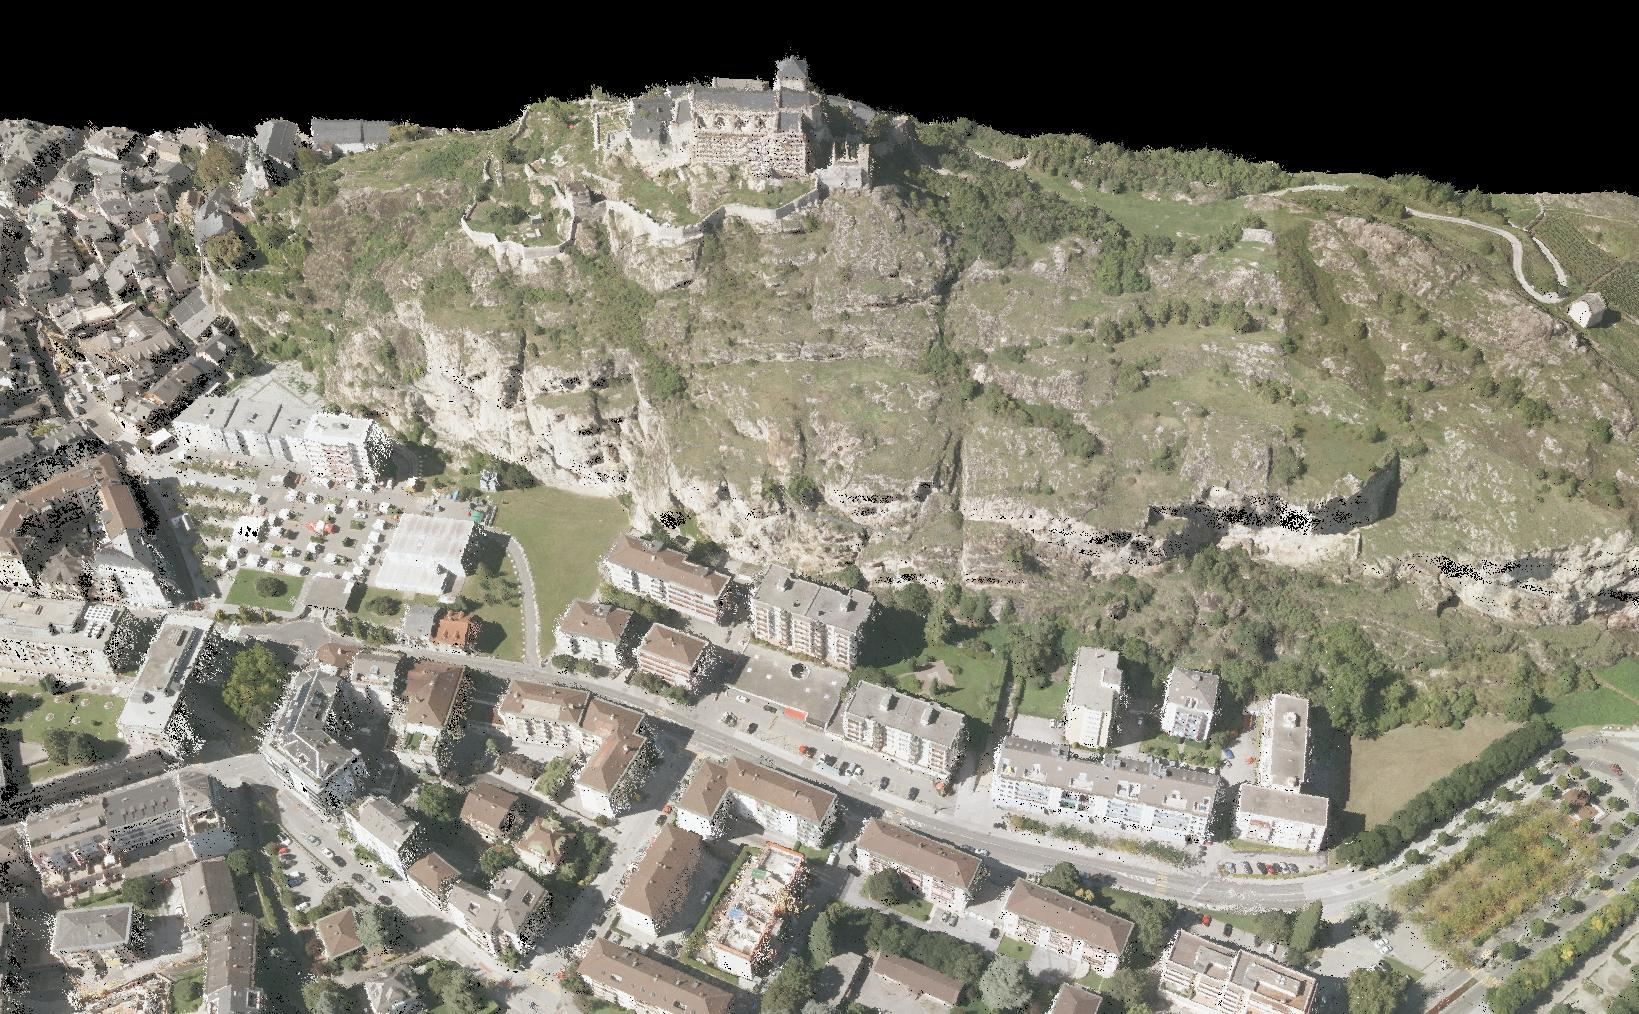
\includegraphics[width=15cm]{ScanVan.jpg}
\caption{Ville de Sion, compilée par ScanVan \textit{© Copyright EPFL DHLAB}}
\end{figure}
Iconem\footnote{\cite{iconem_iconem_nodate}}, start-up partenaire du projet, s'est spécialisée dans la numérisation de sites patrimoniaux en danger, grâce à des drones et à des processus de \gls{photo}. Par la mise en commun de ces développements technologiques, Time Machine vise à la création et à l'implémentation d'un système des plus efficients.
%==========Deuxième technologie ==================
\item \textbf{Extraction et indexation des informations contenues} 

On peut déterminer différentes étapes dans les traitements d'un document après sa numérisation et la liste tend à s'agrandir. On parle notamment : de l'automatisation des processus de repérages du texte ou des motifs au sein d'une image, de la compréhension de l'architecture du document par le biais des technologies du \gls{tal}, de la \gls{ree}, ou encore des technologies liées à la \gls{reo}.

 La plupart des projets du \gls{dhlab} conduisent des recherches dans ces domaines, c'est le cas notamment de \textit{DHSegment}\footnote{\cite{epfl.dhlab_introduction_nodate}} cité pour le projet vénitien ou du projet \textit{Impresso - Media monitoring of the past (2017-2020)}\footnote{\cite{epfl.dhlab_2017-2020_nodate}}, visant à automatiser l'extraction des informations de 200 ans d'archives de journaux afin d'en faciliter la recherche et la découverte. 

Les différentes technologies déployées dans le cadre de ces deux projets seront amenées à enrichir les futurs composants de la Time Machine. Il n'existe actuellement qu'un nombre limité d'applications d'\gls{appr} pour le traitement des données culturelles et patrimoniales. Time Machine entend développer un réseau de chercheurs et de projets visant à améliorer cet existant\footnote{Dans le cadre du stage, nous avons produit différents états de l'art sur les technologies déployées dans Time Machine, ces informations sont contenues dans la feuille de route, figurant sur la clé USB accompagnant ce mémoire.}.
\begin{figure}[H]% force à placer l'image au sein de notre balise figure
\centering

\includegraphics[width=15cm]{impresso.jpg}
\caption{Impresso, visuel \textit{© Copyright 2019 EPFL, DHLAB}}
\end{figure}
%==========Troisième technologie ==================
\item \textbf{Extrapolation - simulation des données depuis d'autres sources} 

L'une des dimensions caractéristique des \textit{\gls{bigd}}, est celle dite paradigmatique. Le nombre de données permettent elles-mêmes de déduire de nouvelles formes de sciences et de faire des découvertes\footcite{kaplan_big_2017}. Ce processus s'apparente à celui mis en place par les moines copistes ou historiens confrontés à devoir \inquote{combler les trous} de l'histoire et faire communiquer entre elles des sources différentes. Ce travail suscite depuis longtemps de nombreux débats sans qu'il existe de normes sur la manière de procéder. Time Machine soutient à priori qu'il faut veiller à précisément documenter ces techniques et les moyens déployés pour parvenir à cette \inquote{redocumentation} du passé\footcite{kaplan_big_2017}. Face aux immenses jeux de données que sont les \textit{\gls{bigd}}, les machines ont un rôle important à jouer dans la détermination du plus petit dénominateur commun capable de réunir différentes interprétations de l'histoire\footcite{kaplan_big_2017}.

Basé sur les méthodologies de l'\gls{ia}, trois moteurs de simulation, dont un moteur d'inférence permettront à Time Machine de déduire de nouvelles informations des données numérisées.

Les moteurs d'inférence ou \textit{Inference Engine} étaient un champ d'étude en \gls{ia} très populaire ; les technologies liées à l'\gls{appr} ont quelque peu réduit l'intérêt des chercheurs en la matière\footnote{Dans le cadre du stage, nous avons produit différents états de l'art sur les technologies déployées dans Time Machine, ces informations sont contenues dans la feuille de route, donnée en annexe sur la clé USB accompagnant le présent mémoire}. Time Machine entend relancer cette recherche et utiliser les données produites pour accroître son \gls{graph} de données du passé.
%==========Quatrième technologie ==================
\item \textbf{Valorisation des données afin de transformer le patrimoine en un atout pour les industries et l'économie européenne}

Afin de faciliter la découverte des données assemblées par Time Machine, une seule interface sera utilisée pour leurs valorisations, rassemblant en back-office tous les processus développés pour le projet\footnote{\cite{epfl.dhlab_dh_2019}}. 

Une première version de la future interface existe et est en cours de développement au sein du \gls{dhlab}. Cette dernière sera amenée à changer énormément au fil des avancées du projet afin de devenir un moteur de recherche diachronique : Diamond\footnote{\cite{time_machine_diamond_nodate}}.
Inclure la temporalité au sein du futur moteur de recherche implique pour Time Machine de favoriser les recherches menées sur la création de modèle 4D, actuellement dévouées à de petites échelles sans faire l'objet de standardisation\footnote{Dans le cadre du stage, nous avons produit différents états de l'art sur les technologies déployées dans Time Machine, ces informations sont contenues dans la feuille de route, figurant sur la clé USB accompagnant ce mémoire.}.
\end{enumerate}
\newpage
\begin{figure}[H]% force à placer l'image au sein de notre balise figure
\centering
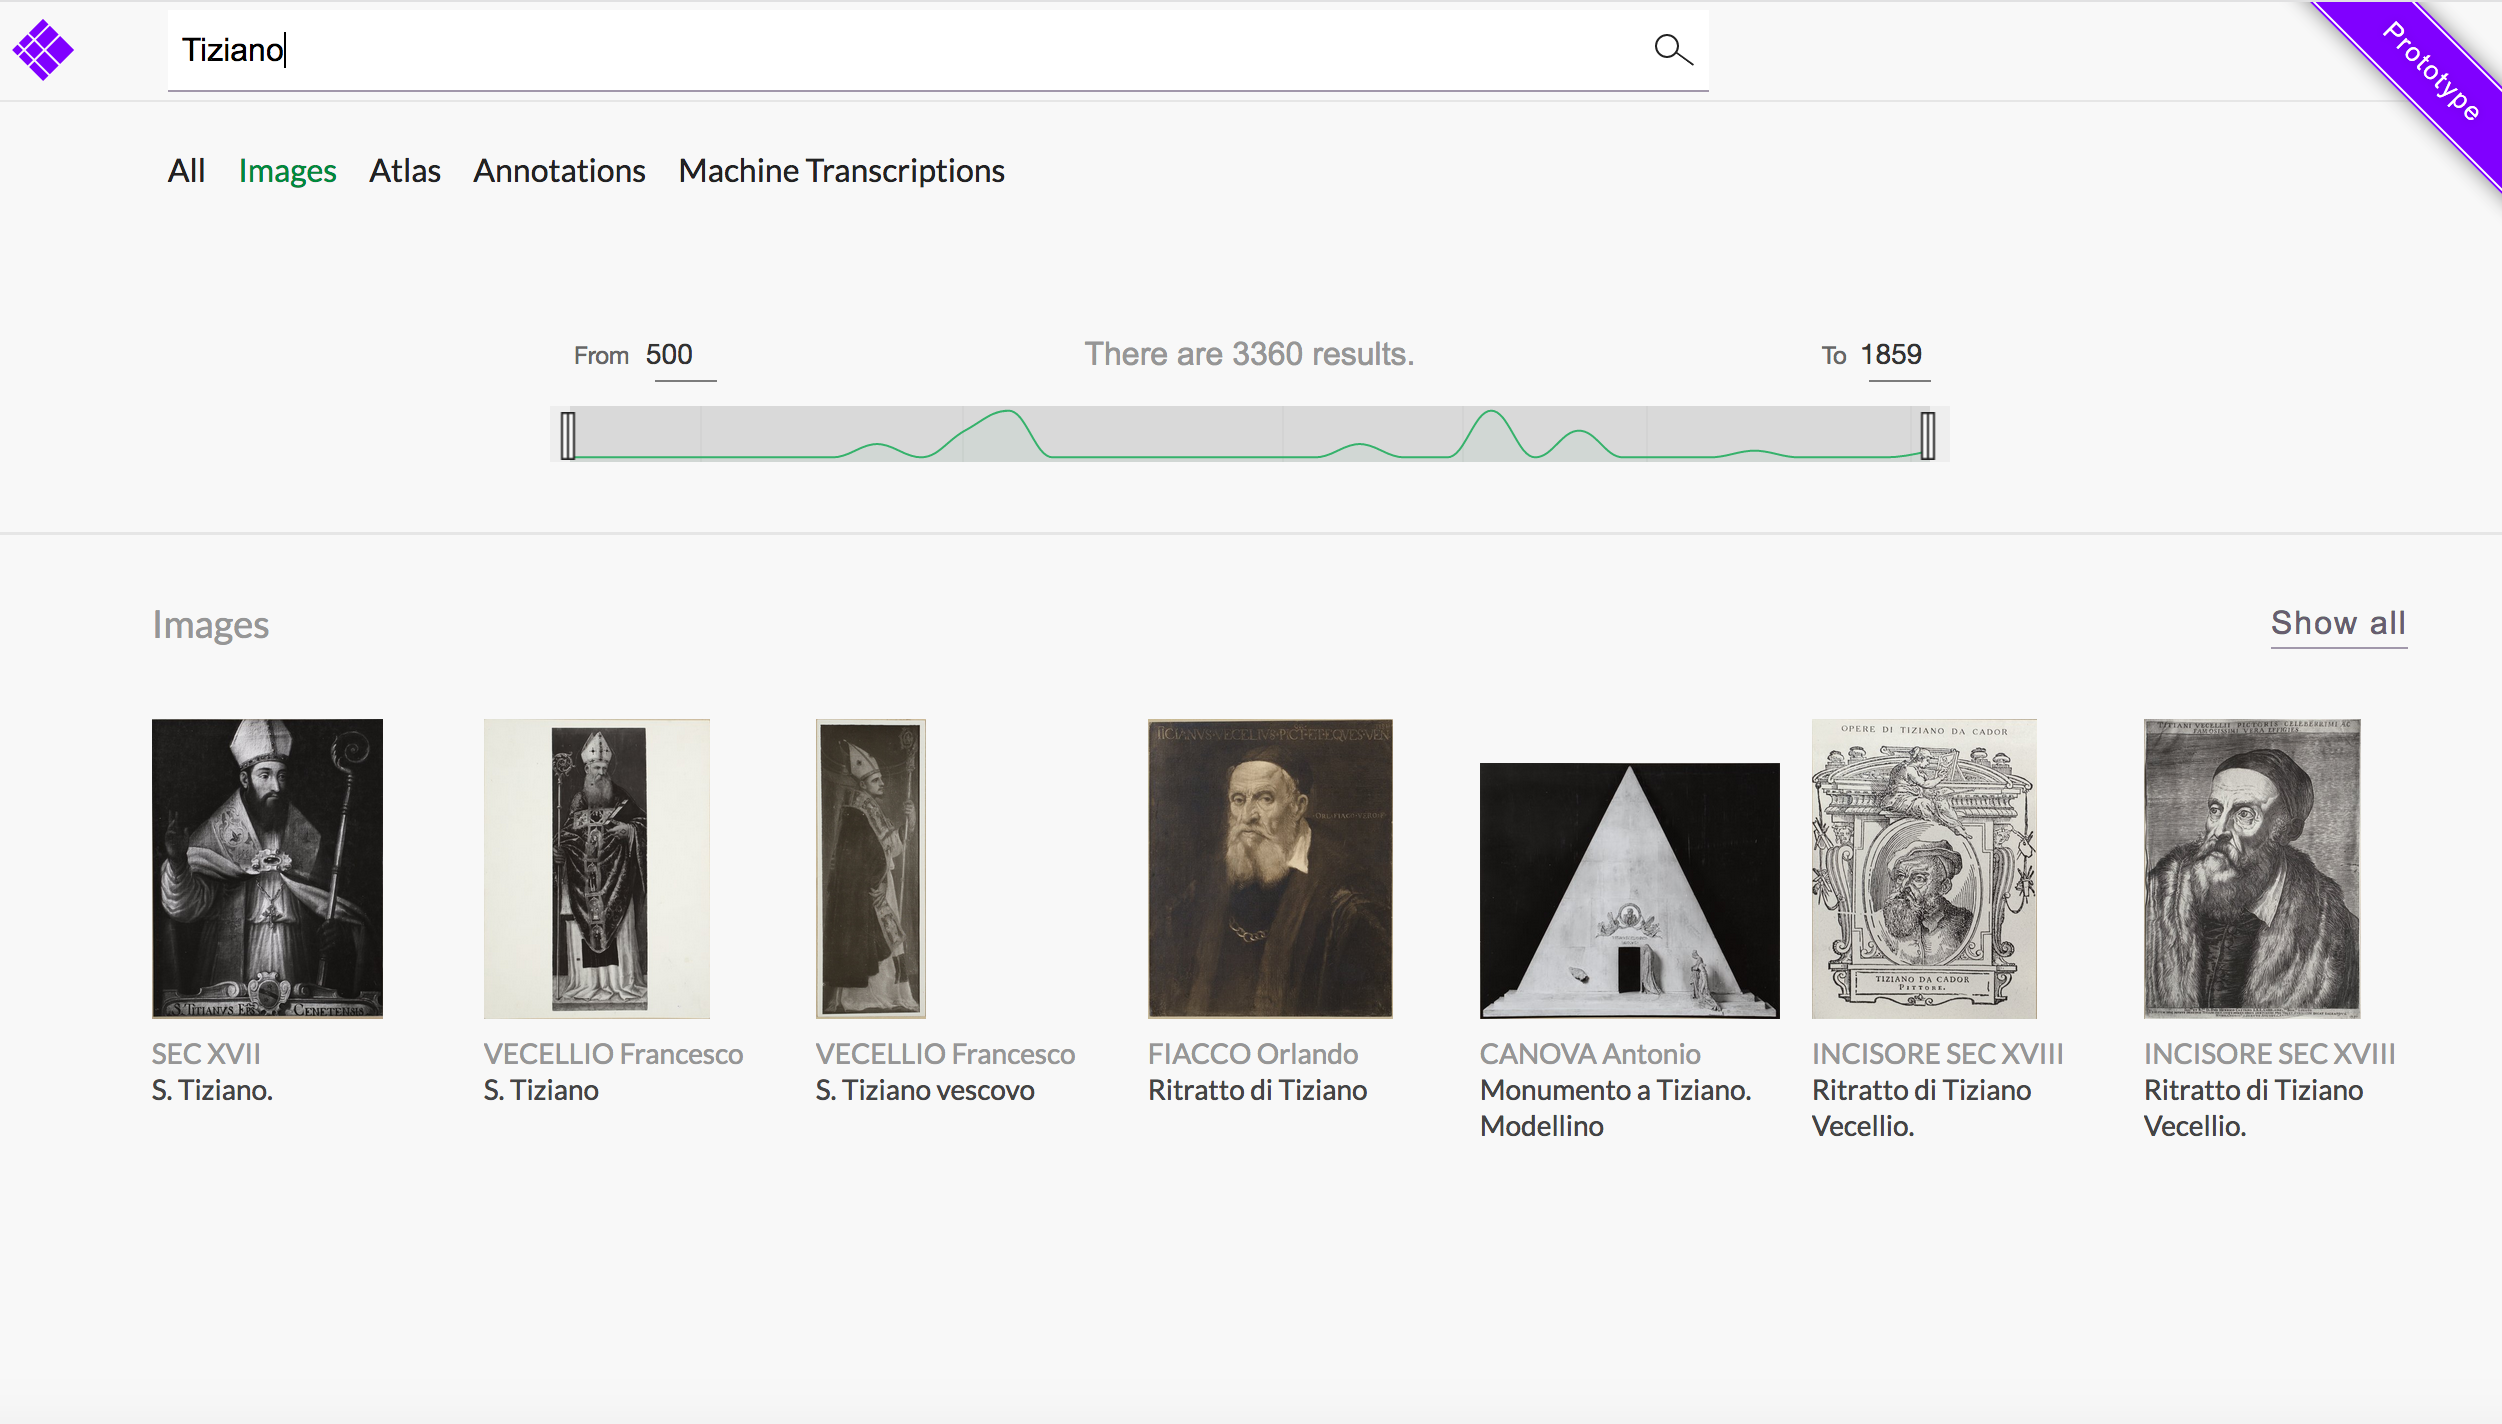
\includegraphics[width=14cm]{diamond.png}
\caption{Interface de Diamond, capture d'écran \textit{© Copyright 2019 Time Machine}}
\end{figure}

\begin{figure}[H]% force à placer l'image au sein de notre balise figure
\centering
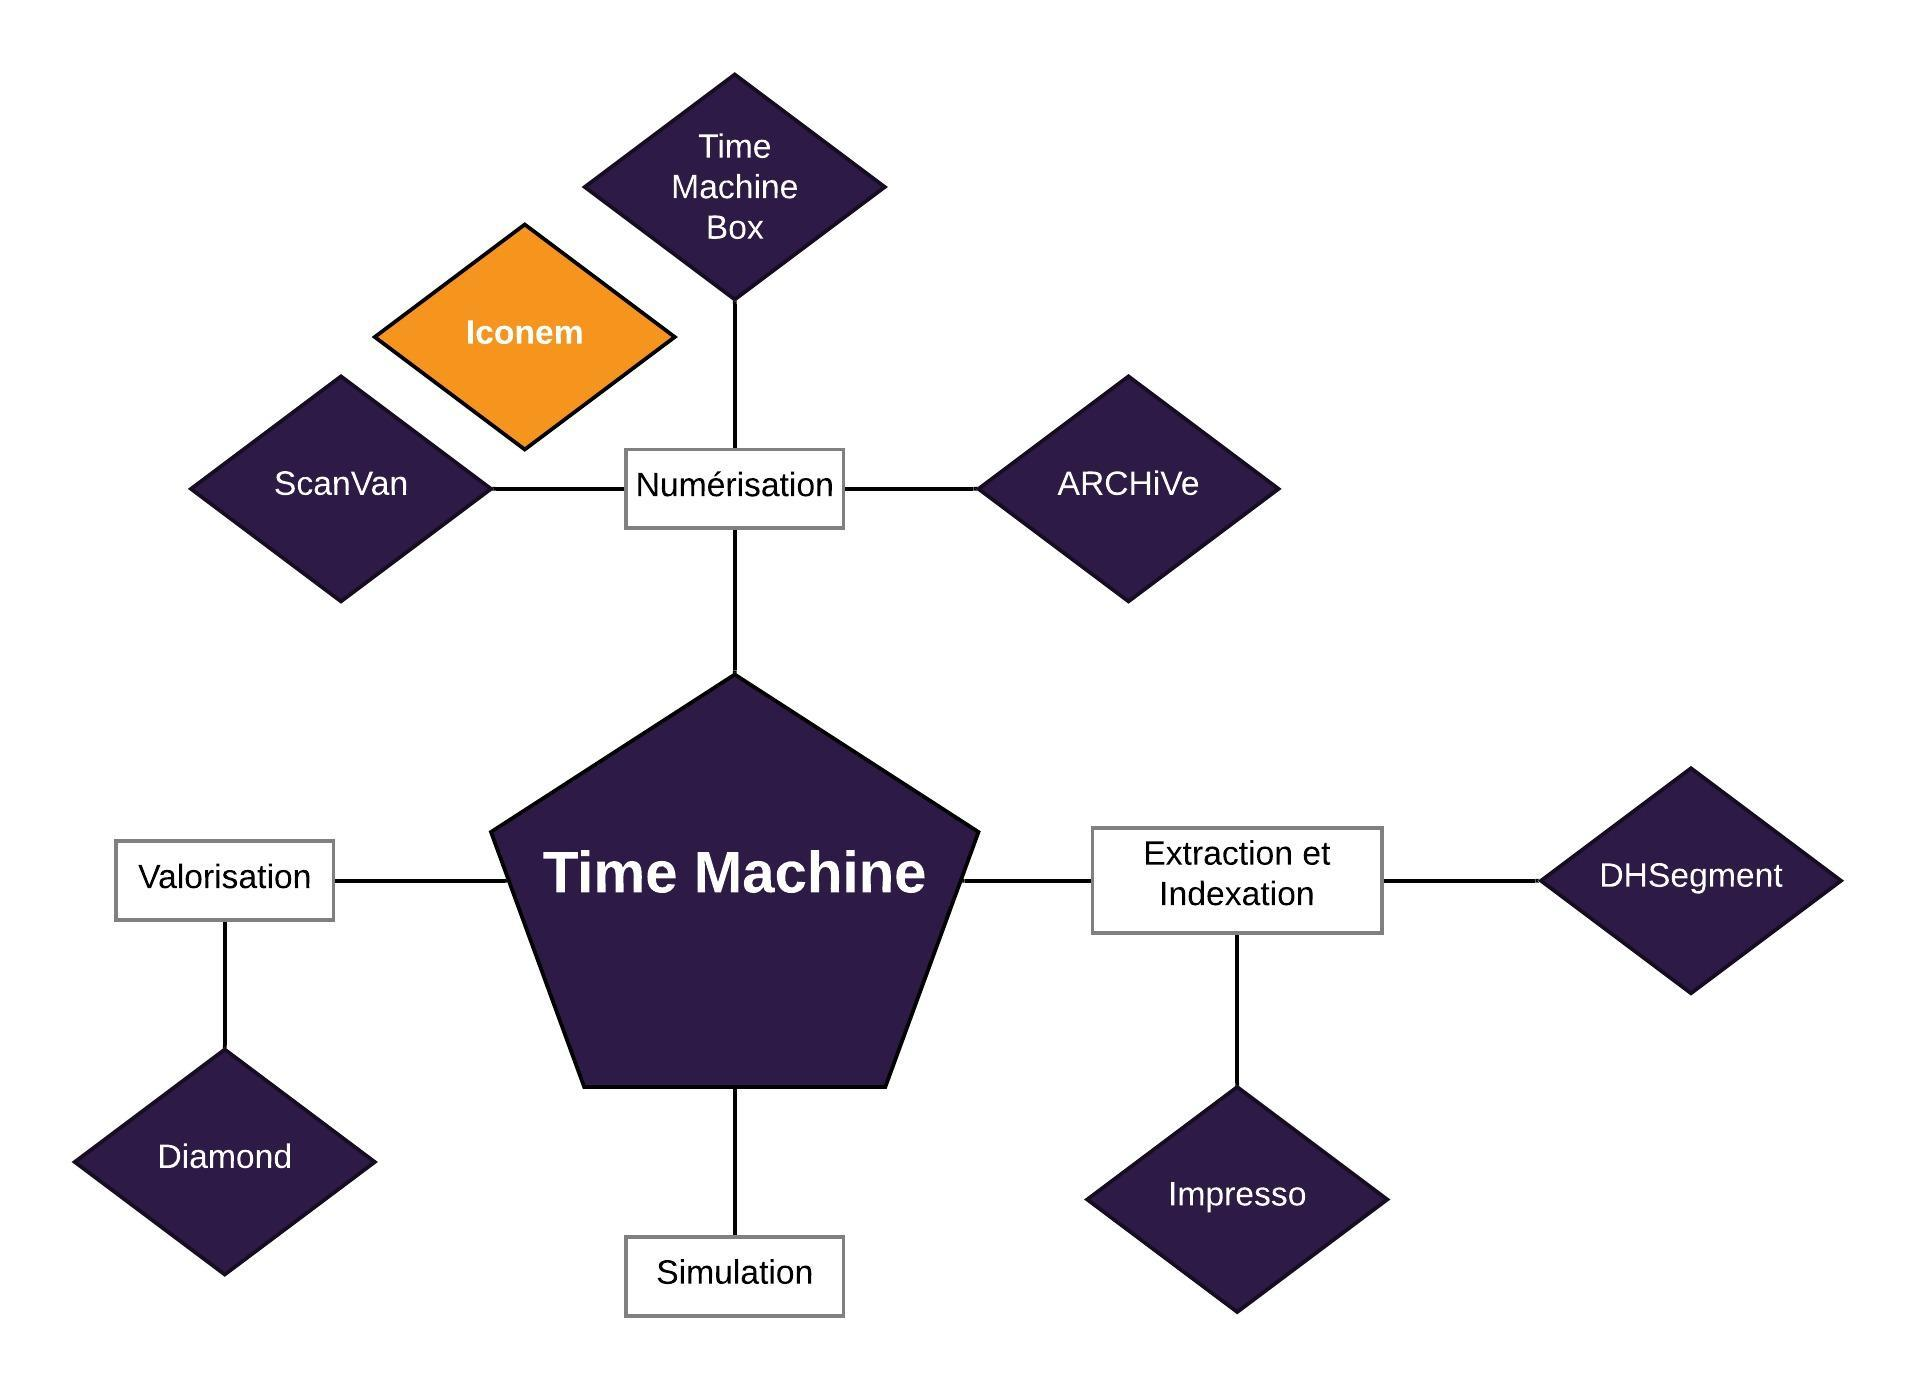
\includegraphics[scale=1.05]{technos.jpeg}
\caption{Résumé visuel des projets et technologies évoqués}
\end{figure}

\subsection{Collaboration public-privé de partenaires européens}
Des 32 partenaires initialement impliqués dans Time Machine, le consortium s'est désormais agrandi à plus de 300 institutions réparties dans 34 pays et les chiffres continuent de croître. Notre stage nous a amené à en côtoyer un grand nombre\footnote{Notamment lors de la conférence à Amsterdam, d'un séjour à Venise pour découvrir les coulisses du projet vénitien et des contacts nécessaires à la création de la feuille de route.} et offert la possibilité de questionner leurs motivations de manière informelle. De nos observations sur le terrain et de part nos activités de stagiaire, nous proposons d'établir certaines typologies, afin de mieux appréhender la multiplicité des profils et des attentes à l'encontre du projet. N'ayant pu mener de réelle étude quantitative, nous ne prétendrons pas être exhaustif : \footnote{\cite{time_machine_introduction_nodate}}. 
\begin{itemize}
\item \textbf{Les institutions culturelles et patrimoniales}

Composées de représentants des \gls{glam}, ces dernières sont à la fois intéressées par les traitements de numérisation appliqués à leurs données et par l'exploitation des résultats pour leurs propres besoins de valorisation auprès de leurs publics-cibles.
\item \textbf{Les réseaux ou consortiums}

Composés d'associations d'envergure actives dans le milieu du patrimoine, à l'instar d'Europeana\footnote{\cite{noauthor_europeana_nodate}} ou d'Icarus\footnote{\cite{icarus_icarus_nodate}}, ces dernières sont intéressées à intégrer un réseau qui leur permet à la fois de transcender leurs domaines d'activités, de rendre visibles leurs actions, d'accroître leurs membres et de participer au déploiement d'innovations technologiques applicables au sein de leurs communautés.
\item \textbf{Les laboratoires de recherche ou universités}

Composés de représentants des sciences humaines et sociales aussi bien que des sciences dures, ces centres de recherches sont motivés à l'idée de prendre une part active dans les processus d'élaboration des différents composants techniques et de traitement de ce \textit{\gls{bigd}} du passé. Ils sont également intéressés à déployer les résultats dans leurs missions d'enseignement.
\item \textbf{Les start-ups et entreprises privées}

Actives dans les domaines innovants impliqués dans Time Machine, ces dernières sont intéressées à développer de nouveaux services et modèles d'entraînement grâce aux données du \gls{graph} du passé et à valoriser ou accroître leurs compétences au sein d'un réseau de grande envergure.
\item \textbf{Les futurs exploitants}

Le \gls{graph} une fois constitué laissera la possibilité à un grand nombre d'acteurs de créer leurs propres plateformes ou services basés sur ce \textit{\gls{bigd}} du passé. Nous retrouvons ici, aux côtés des villes et des représentants des régions (le \textit{\gls{bigd}} faisant écho au mouvement des \textit{smart cities\footnote{Une ville intelligente utilise les données collectées sur internet pour mieux gérer et planifier l'utilisation de ses ressources.}}), les industries culturelles et créatives, à l'instar du fabriquant de jeu vidéo Ubisoft\footnote{\cite{ubisoft_welcome_nodate}}, les industries du tourisme, de la recherche et de l'éducation, tous intrigués par la perspective de construire de nouveaux lendemains grâce à ces données du passé.
\end{itemize}

\subsection{Un réseau de Time Machines locales}
A l'instar de Venise, d'autres villes n'ont pas attendu la fin du processus de financement pour se lancer dans la construction de leurs propres Time Machines locales. Poursuivant des objectifs divers en fonction de leurs particularités régionales et de la temporalité de leurs archives, ces initiatives sont amenées à constituer le centre du futur réseau Time Machine, qui se veut un réseau de Time Machines locales (appelées à jouer un rôle similaire à celui des \gls{agr}s),  composées de divers projets aux spécificités régionales, sous la gouvernance de la future \textit{Time Machine Organisation}. Dans un contexte au financement incertain, elles montrent également que des solutions financières locales et régionales peuvent être trouvées\footnote{\cite{rts_coup_2019}}, dont le futur réseau Time Machine\footnote{\cite{time_machine_local_nodate}}\footnote{La \textit{factsheet} du projet, donnée en annexe \ref{factsheet}, présente une liste des Times Machines locales} n'a pas encore fini d'explorer toutes les possibilités. Nous citerons ici quelques exemples parmi d'autres : 
\begin{enumerate}
\item Antwerp Time Machine (1500 - 2000)\footnote{\cite{university_of_antwerp_antwerp_nodate}}
\item Amsterdam Time Machine (1550 - 2000)\footnote{\cite{amsterdam_time_machine_amsterdam_nodate}}
\item Budapest Time Machine (1680-1990)\footnote{\cite{hungaricana_budapest_nodate}}
\item Dresden Time Machine (1200 - 2000)\footnote{\cite{noauthor_dresden_nodate}}
\item Paris Time Machine (1000 - 2000)\footnote{L'École Nationale des Chartes est membre du projet.}
\end{enumerate}

\begin{figure}[H]% force à placer l'image au sein de notre balise figure
\centering
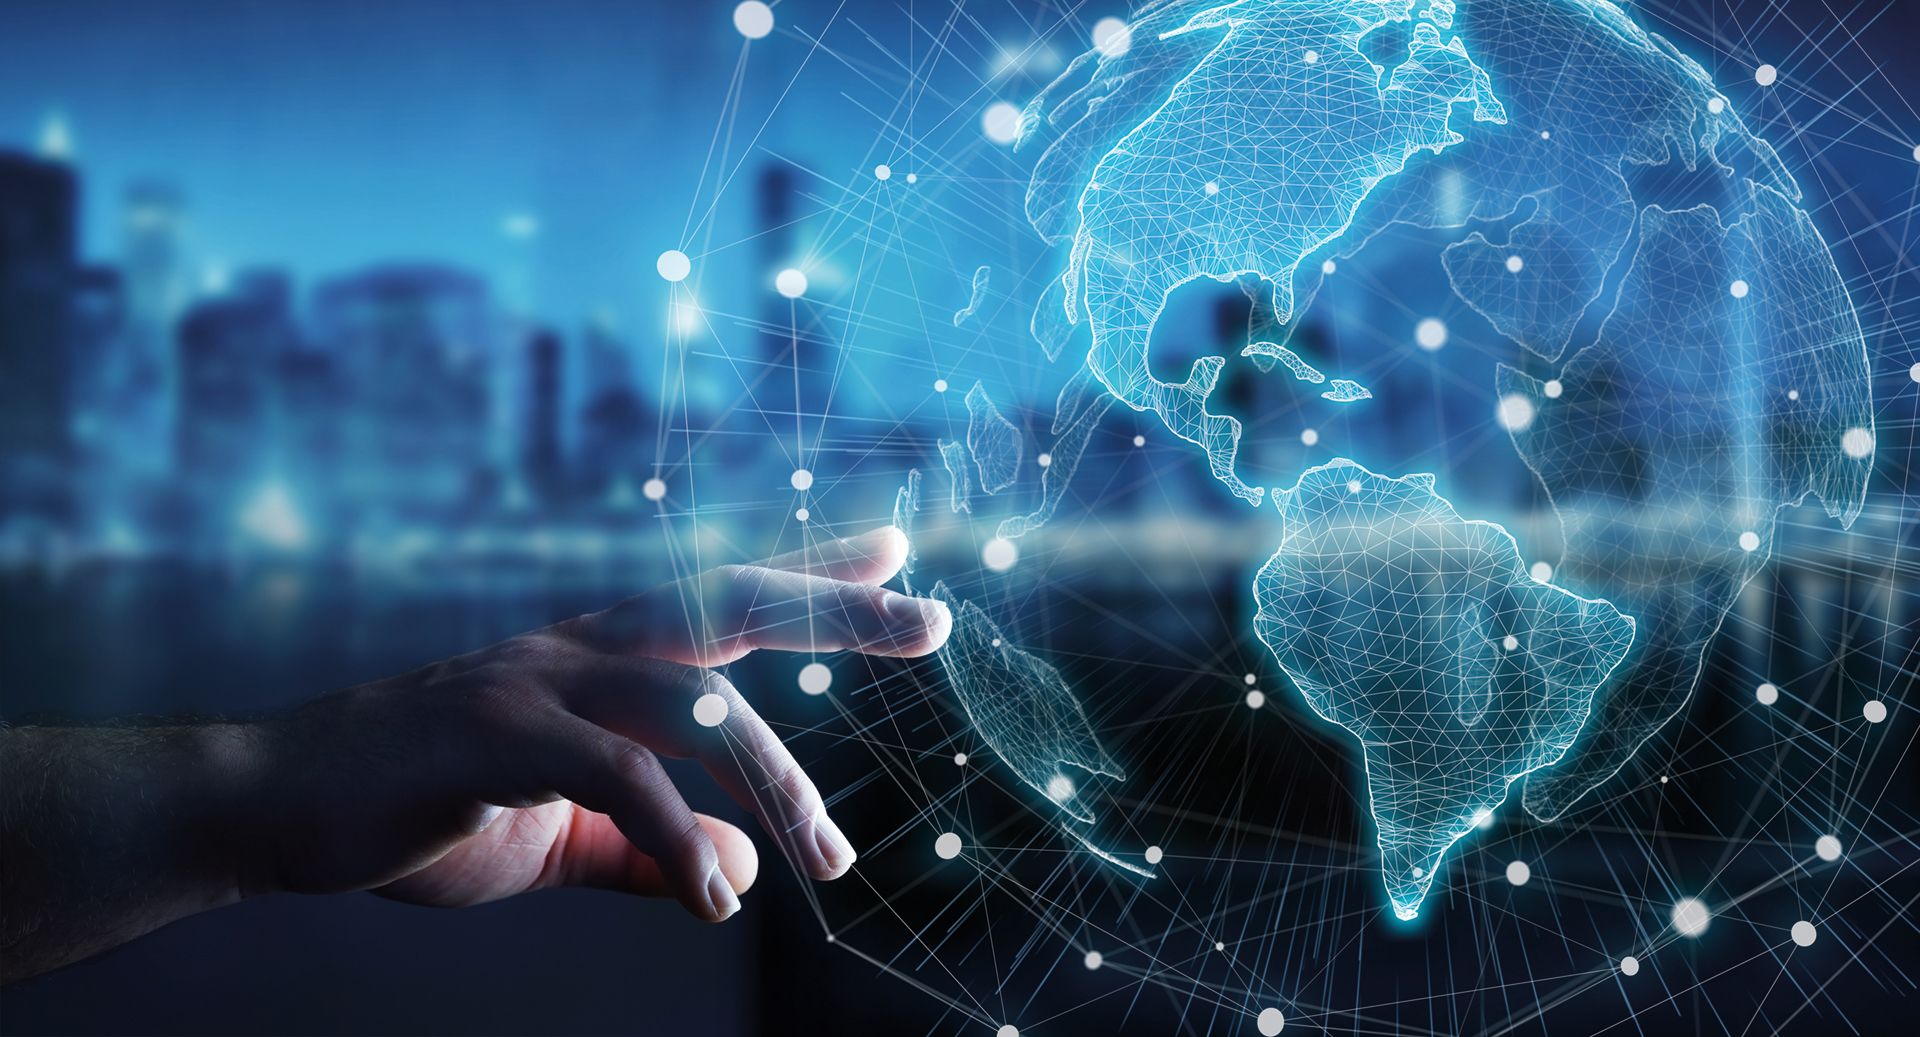
\includegraphics[width=15cm]{data_tm.jpg}
\caption{Time Machine, visualisation du réseau \textit{© Copyright 2019 Time Machine}}
\end{figure}


\part{Exemples de projets de numérisation de masse }

\chapter{Différentes typologies de projets}

Afin de mieux appréhender les réponses des projets de numérisation de masse aux enjeux de la numérisation et de mieux comprendre leurs similitudes et divergences, nous allons en présenter quatre encore actifs aujourd'hui. Pour rappel, nous exposerons dans la troisième partie de ce mémoire, les solutions proposées pour Time Machine. Suivant les recommandations de Margaret Coutts, nous distinguons deux typologies parmi ces exemples\footcite{coutts_stepping_2017}. 

\textbf{Typologie 1} : Les premières initiatives présentées (\textit{Google Books} et \textit{HathiTrust}), ont pour objectif de rassembler en ligne des corpus massifs de données numérisées. Aux côtés d'autres initiatives que nous ne détaillerons pas dans ce mémoire, telles que \textit{Microsoft Live Book Search}\footnote{Le projet s'étant arrêté en 2008, le contenu est désormais accessible à travers la plateforme d'\textit{Internet Archive : https://archive.org/index.php}} ou \textit{the Open Content Alliance}\footnote{Initié en 2005, ce groupe a rassemblé des institutions privées (Yahoo!), et publiques (\textit{Perseus Digital Library}) pour proposer une alternative aux objectifs commerciaux de Google. Ils étaient administrés par \textit{Internet Archive}, dont le fondateur Brewster Kahle est un militant pour l'accès universel à la connaissance via la numérisation et un opposant au projet de Google : https://archive.org/details/opencontentalliance. Le consortium ne semble plus actif depuis 2009.}, ils ont fortement contribué à l'accroissement des données numérisées et au développement de l'expertise technique nécessaire à la gestion de telles collections\footcite[p.78]{coutts_stepping_2017}.

\textbf{Typologie 2} : Les deuxièmes, bien que soutenant des entreprises de numérisations au sein de leur réseau, visent surtout à rassembler les données numérisées par de multiples institutions et les mettre à disposition via une interface commune : ce sont les \gls{agr}s (Europeana, \textit{\gls{dpla}}). Ces \gls{agr}s se caractérisent par une architecture distribuée, terme désignant un réseau informatique dont l'ensemble des ressources ne se trouvent pas au même endroit ou sur la même machine, mais sont stockées sur les serveurs de leurs institutions\footcite[p.79]{coutts_stepping_2017}.

Nous ne parlerons pas d'une autre forme d'initiatives visant à rassembler en ligne des corpus de données numérisées, les \textit{shadow libraries}. Ces bibliothèques \inquote{de l'ombre}, sont devenues des infrastructures de numérisation à grande échelle et proposent un accès gratuit et souvent illégal à des livres et articles académiques\footcite{thylstrup_politics_2018}. Caractérisées par une construction fragile voire éphémère, elles constituent un phénomène digne d'intérêt, mais que nous avons choisi de ne pas aborder afin de ne pas trop alourdir notre mémoire.

Si les typologies proposées par Margaret Coutts s'articulent autour de la construction des projets, elles font toutefois écho à celles mentionnées dans les sections \ref{echelle} et \ref{caracteristique}, qui évoquaient des critères différenciant initiatives publiques et privées. 

Pour pouvoir mieux comprendre les débats autour de ces efforts de catégorisation ou de classement des projets de numérisation de masse\footnote{\cite[p.245]{jones_public_2017}}, nous nous intéresserons également à leurs origines et motivations. Nous proposons un résumé comparatif des différentes réponses apportées aux enjeux de la numérisation et une brève conclusion à ce débat dans le chapitre \ref{distinction}.

%======NUMERISER EN MASSE
\section{Rassembler une masse de données numérisées}
%======Google Books (google ou exemple)
\subsection{Google Books}
Le projet initié en 2004 sous le nom de \textit{Google Print}, qui deviendra \textit{Google Partner Program}, a pour objectif de rendre accessible tout ce qui a été écrit par l'homme sans distinctions\footcite{thelle_persuasive_2011}. Les fondateurs de l'entreprise Larry Page et Sergey Brin annoncent à la foire du livre de Francfort la création d'une nouvelle plateforme d'édition pour permettre aux auteurs et éditeurs de commercialiser en ligne leurs ouvrages.

En complément de la création de cette plateforme d'édition, le \textit{Google Library Project}, qui vise à numériser sur dix ans, quelque 15 millions d'ouvrages à la fois libres et sous droit est lancé la même année. Cinq bibliothèques de langue anglaise sont partenaires de cette première étape du projet : celle de l'Université du Michigan, Stanford, Harvard, Oxford (Bodleian) et la bibliothèque publique de New York\footcite{thylstrup_politics_2018} \footcite{weiss_assessing_2013}. 

Afin d'uniformiser les deux programmes qui travaillent à la réalisation du même objectif, le \textit{Google Partner Program} et le \textit{Google Library Project}, changent de nom en 2005 pour se rassembler derrière la bannière de \textit{Google Books}.

Google retire de nombreux avantages de son projet de création de cette future bibliothèque universelle : des données pour contribuer à la réalisation d'une \gls{ia} capable de comprendre toute la symbolique humaine, de nouveaux espaces publicitaires, une offre commerciale de livres numérisés\footcite{dufrene_numerisation_2013}.

La mise en \oe{}uvre du projet va très vite se heurter à des barrières d'ordre légal (comment  numériser en restant dans la légalité du droit d'auteur américain), technique (quels moyens déployer pour numériser à grande échelle et comment valoriser et organiser ces données) et politique (comment dépasser les limites de fonctionnement territoriales et régionales).

Les éditeurs initialement du côté de Google vont prendre peur en constatant que ce dernier numérise également les ouvrages des bibliothèques. S'ensuivront différents procès et le lancement des débats liant droit d'auteur et numérique. Toutefois Google gagnera successivement ces derniers, grâce au principe du \textit{fair use}\footnote{Pour rappel, le \textit{fair use} autorise cinq exceptions au droit d'auteur : le droit à opérer une copie privée, le droit de citation, le droit au pastiche ou à la caricature, l'usage pour l'enseignement, l'usage pour la recherche.} états-unien, contribuant à créer les bases légales légiférant la circulation des biens culturels et patrimoniaux en ligne\footcite{xie_discover_2016}\footcite{stobo_i_2018}. Google a compris avant tout le monde que \inquote{les barrières techniques classiques à un contournement du droit d'auteur tombaient avec le numérique\footcite[p.37]{dufrene_numerisation_2013}}. 

Il semble que la firme ne dispose pas d'équipe chargée de vérifier les droits d'auteur et qu'en cas de doute, elle préfère directement limiter l'accessibilité. L'utilisateur est informé par des pages introductives multilingues sur les droits d'usage de chaque ouvrage\footcite{leetaru_mass_2008}, ces derniers figurent également dans les métadonnées.

\textit{Google Books} propose une recherche plein-texte gratuite par mots-clés\footcite{leetaru_mass_2008}, limitée par quatre différentes vues en fonction de l'accessibilité des documents. Un accès au texte intégral (le livre peut être téléchargé), un accès à quelques pages donnant un aperçu de l'ouvrage (en accord avec l'éditeur, avec un lien permettant de l'acheter), un accès aux métadonnées et à quelques phrases permettant de comprendre le contexte du mot-clé de la recherche (lorsque la license n'est pas claire) ou un accès uniquement aux métadonnées (lorsque l'ouvrage n'a pas été numérisé)\footcite{hoffmann_google_2016}\footcite{weiss_using_2014}.
\newpage
\begin{figure}[H]% force à placer l'image au sein de notre balise figure
\centering
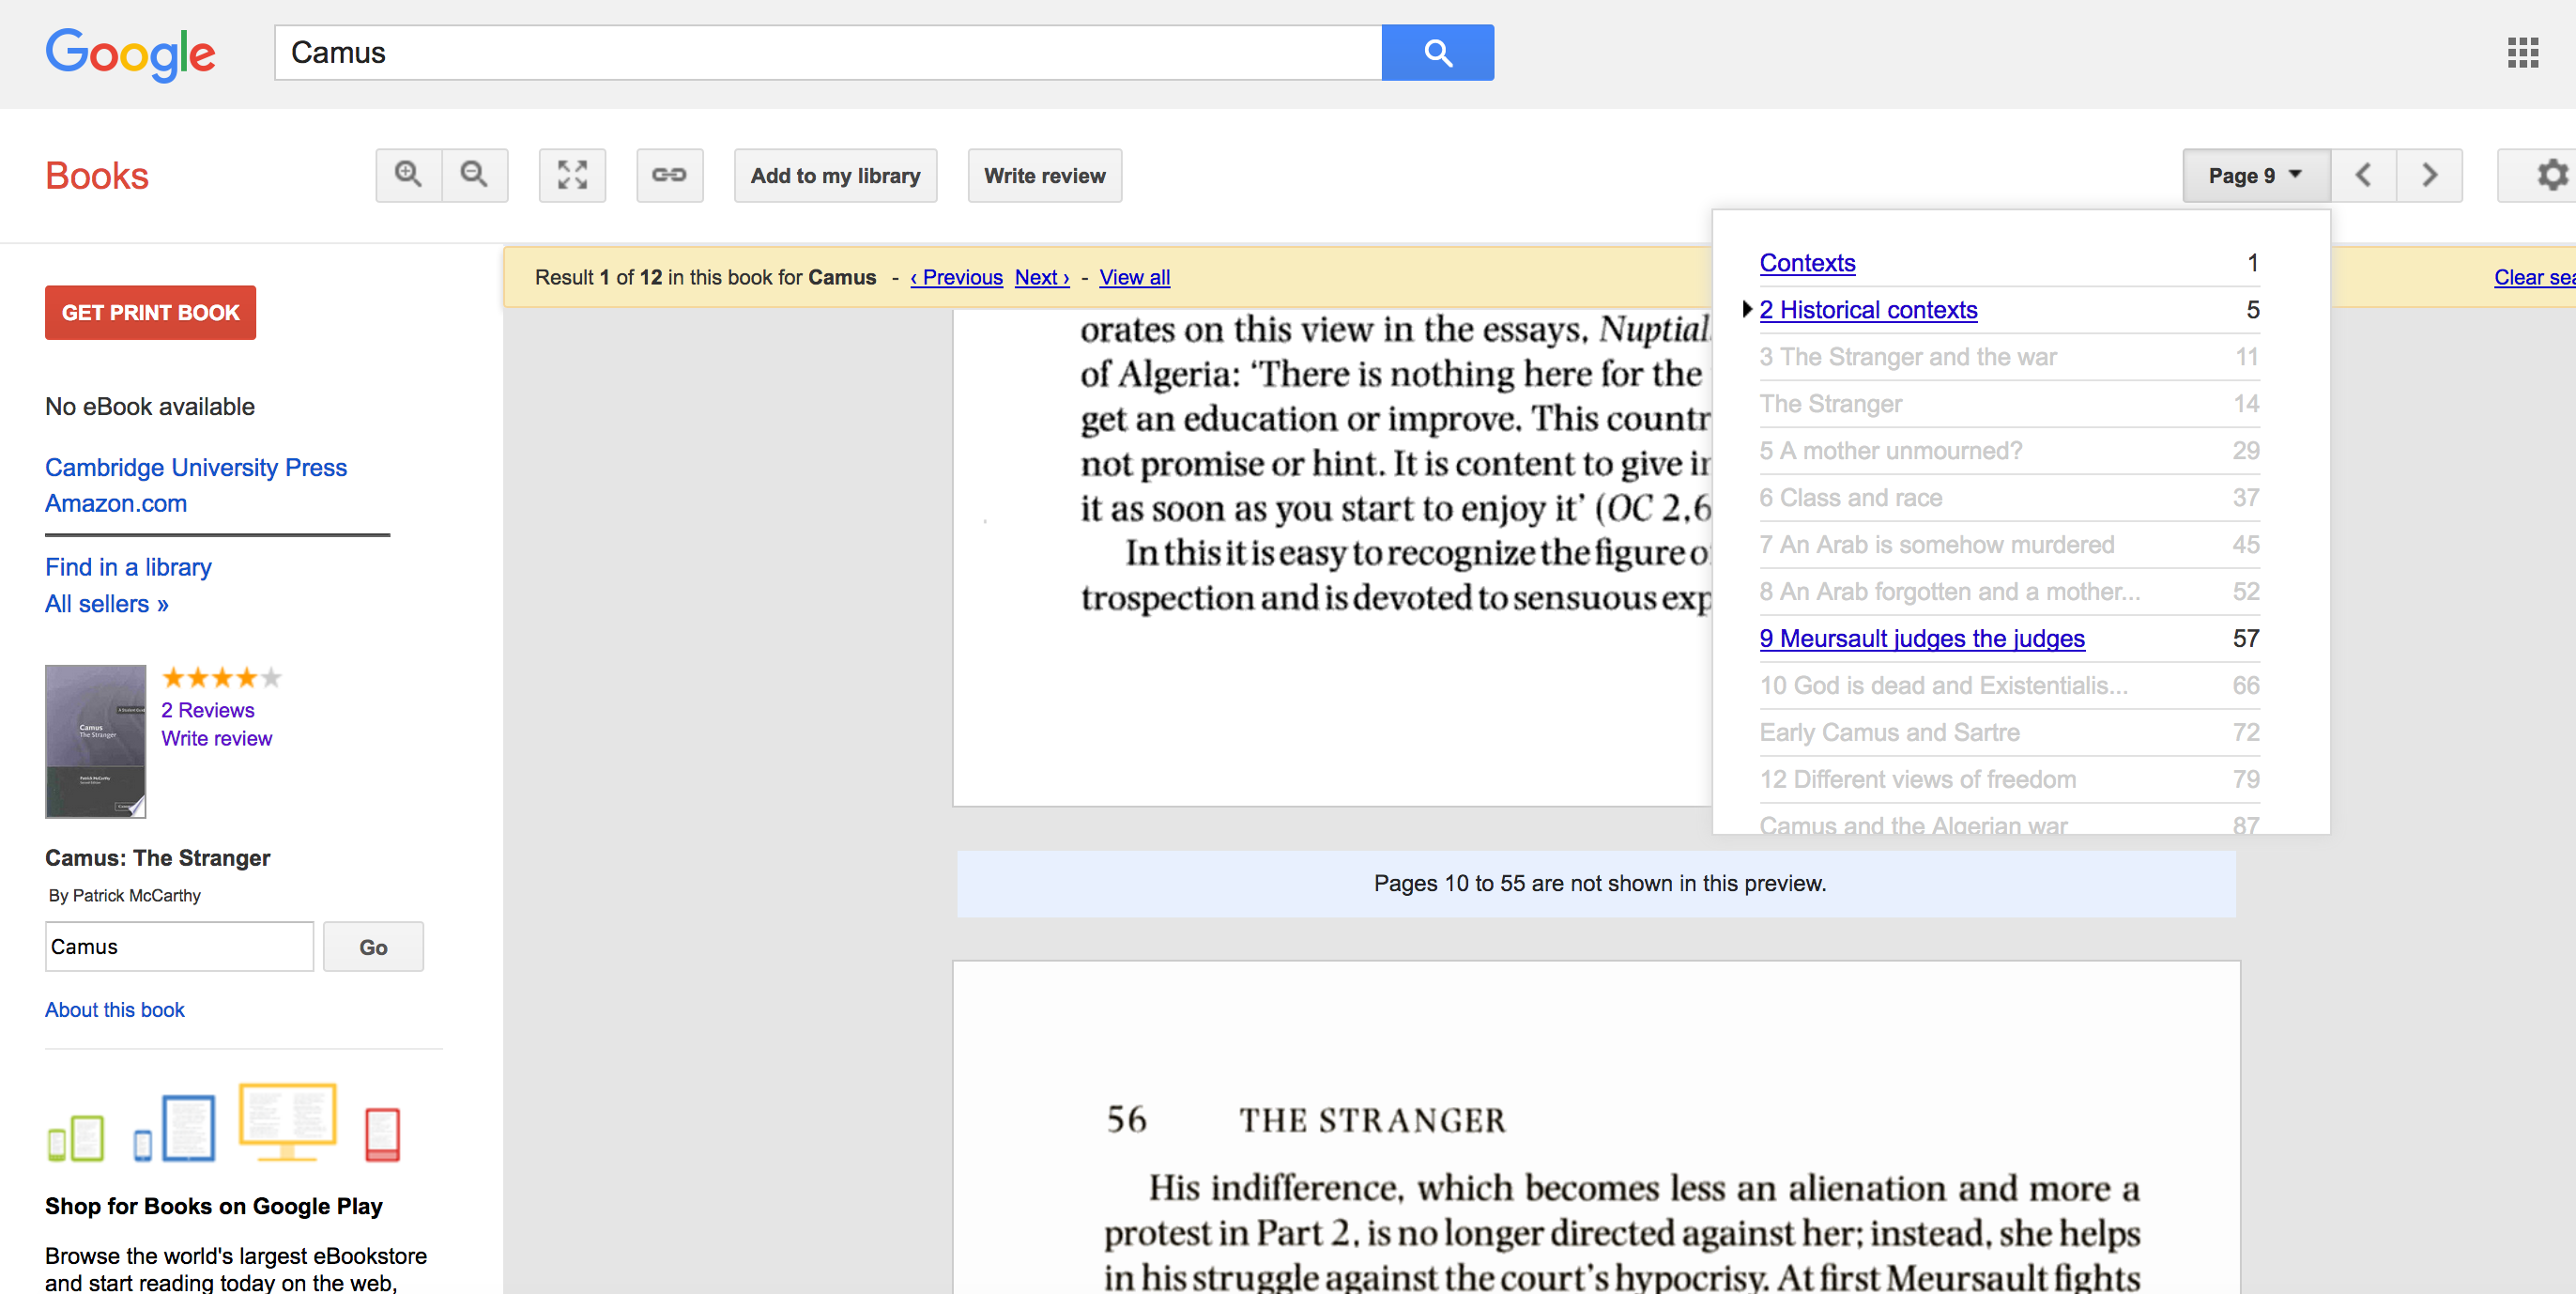
\includegraphics[width=15cm]{googleb}
\caption{Affichage d'un résultat \textit{Google Books}, capture d'écran}
\end{figure}

Passés les débuts rapides et presque \inquote{agressifs} de l'initiative, le droit d'auteur est néanmoins avancé pour justifier le récent ralentissement de l'entreprise et une nouvelle prédilection pour la numérisation d'ouvrages libres de droit\footcite{thylstrup_politics_2018}\footcite{weiss_examining_2016}\footcite{noauthor_viewpoint_nodate}. 

Les débuts sont caractérisés par de nombreux problèmes relatifs à la qualité des métadonnées et des images\footcite{hoffmann_google_2016}. Les langues non romanes sont sous-représentées et les spécificités propres à d'autres histoires littéraires (telles que celles japonaises où les livres sont construits sur d'autres logiques que celles européennes) sont difficilement prises en compte dans les processus de numérisation\footcite{weiss_examining_2016}. Les biais dans la construction des collections sont hérités des bibliothèques partenaires\footcite{weiss_assessing_2013}. De nombreux problèmes sont également constatés concernant la gestion des ouvrages en plusieurs volumes. En vérité, par rapport aux standards élevés des bibliothèques, \textit{Google Books} a du mal à faire concurrence. Cela ne signifie pas qu'il réussit moins bien son objectif de desservir le plus grand nombre, puisqu'il permet d'accéder aux recherches au sein de l'environnement Google.

Google ne partage pas publiquement les processus et les algorithmes de traitement de ces données\footcite{hoffmann_google_2016}. La firme se charge du transport des documents vers le lieu de numérisation, puis restitue les données enrichies une fois numérisées, en garantissant leur intégrité. Certaines bibliothèques témoignent d'un rythme de numérisation de quelques 5000 livres par mois\footcite{association_pour_le_patrimoine_naturel_et_culturel_du_canton_de_vaud_patrimoine_2012}.

La préservation sur le long-terme n'étant pas sa priorité, la firme remet tout de même une copie des fichiers aux institutions afin qu'elles puissent y veiller\footcite{leetaru_mass_2008}, pour autant que ces fichiers demeurent stockés sur les serveurs de l'institution\footcite{association_pour_le_patrimoine_naturel_et_culturel_du_canton_de_vaud_patrimoine_2012}. 

Contrairement aux initiatives publiques, Google n'a pas le souci d'inclure l'usager dans le déploiement de \textit{Google Books}. Il a démontré qu'il était capable de réagir et d'intégrer certaines critiques (notamment celles levées dans les premières années du projet qui reprochaient la mauvaise qualité de la numérisation), mais n'est pas prêt à ouvrir son projet plus largement aux besoins des individus\footcite{jones_public_2017}, qui sont limités au rôle de critiques. Les développements technologiques semblent être prioritaires\footcite{hoffmann_google_2016}. 

Sa quête de profit le pousse également à limiter les usages commerciaux faits par la suite et prévient le référencement des titres numérisés par d'autres moteurs de recherche\footcite{clavert_histoire_2013}\footcite{moatti_bibliotheque_2012}. La firme semble cependant largement autoriser les usages pour la recherche\footcite{leetaru_mass_2008}. 

L'initiative de \textit{Google Books} ne laisse personne indifférent, organisant dès le départ le monde en deux camps, celui des partenaires et celui des opposants. Google est entre-temps devenu un géant de l'information, dont le monopole et le non-respect de la protection des données des utilisateurs suscitent autant la crainte que l'admiration\footcite{clavert_histoire_2013}. De ce clivage va naître la plupart des projets de numérisation de masse du 21\up{e} siècle\footcite{thylstrup_politics_2018}. 

En 2018, quelques \textbf{30 millions} de livres ont été numérisés par cette initiative\footcite{thylstrup_politics_2018} et le fonds continue de croître. 

\newpage

\begin{table}[H]
\centering
\begin{tabular}{|l|l|}
\hline
\rowcolor[HTML]{2E1A46} 
{\color[HTML]{FFFFFF} \textbf{Enjeux}}                                                                                   & {\color[HTML]{FFFFFF} \textbf{Réponses de Google}}                                                                                                                                                                                                                                                                                                                                                                                                                                                                                                                                                         \\ \hline
{\color[HTML]{2E1A46} \textbf{\begin{tabular}[c]{@{}l@{}}Amener différents\\ acteurs à collaborer\end{tabular}}}         & \begin{tabular}[c]{@{}l@{}}Chaque contrat est négocié au cas \\ par cas, mais Google impose certaines règles.\\ Un contrat avec Google n'empêche pas la \\ poursuite d'autres projets de numérisation mais \\ prévient certains usages commerciaux.\end{tabular}                                                                                                                                                                                                                                                                              \\ \hline
{\color[HTML]{2E1A46} \textbf{\begin{tabular}[c]{@{}l@{}}Financement et \\ partenariats \\ public-privé\end{tabular}}} & \begin{tabular}[c]{@{}l@{}}Les profits générés par Google suffisent à couvrir les\\ frais des projets de numérisation. Nul besoin de \\ trouver d'autres partenariats financiers.\end{tabular}                                                                                                                                                                                                                                                                                                                                                                                                            \\ \hline
{\color[HTML]{2E1A46} \textbf{Droit d'auteur}}                                                                           & \begin{tabular}[c]{@{}l@{}}Google a gagné plusieurs procès contre la guilde \\ des auteurs aux États-Unis. Toutefois, ces attaques\\ incessantes sont souvent évoquées comme raison \\ aux choix de numériser des ouvrages libres de droit, \\ caractérisant les plus récentes initiatives.\end{tabular}                                                                                                                                                                                                                                                                                                  \\ \hline
{\color[HTML]{2E1A46} \textbf{\begin{tabular}[c]{@{}l@{}}Sortir des silos : \\ enjeux techniques\end{tabular}}}          & \begin{tabular}[c]{@{}l@{}}Déploiement de centres de numérisation et dépôt \\ de divers brevets visant à accélérer les processus \\ (scanners, mélodie aidant à la concentration, \\ automatisation etc.).\\ Si Google est plutôt transparent sur les contrats de \\ numérisation, il protège farouchement les \\ technologies associées, les centres de numérisation \\ ne sont pas visitables. Comme le projet est inclus dans\\ l'environnement de recherche le plus utilisé, les \\ ouvrages numérisés bénéficient d'une grande\\ visibilité et sont accessibles dans plusieurs langues.\end{tabular} \\ \hline
{\color[HTML]{2E1A46} \textbf{\begin{tabular}[c]{@{}l@{}}Sortir des silos : \\ enjeux sur le \\ contenu\end{tabular}}}   & \begin{tabular}[c]{@{}l@{}}Alors même que le projet a pour objectif de tout\\ numériser, sans sélection préalable, certains choix\\ ont été faits, qui le sortent de cette neutralité.\\ En choisissant les plus grands et prestigieux\\ établissements culturels, Google a reproduit \\ leurs biais, privilégiant les ouvrages scientifiques et \\ classiques au détriment de la littérature populaire. \\ Le projet se consacre également à la seule \\ numérisation de livres et privilégie les partenariats \\ avec des institutions dont les ouvrages sont en langue\\ romane.\end{tabular}          \\ \hline
{\color[HTML]{2E1A46} \textbf{\begin{tabular}[c]{@{}l@{}}Stockage sur le \\ long-terme - \\ préservation\end{tabular}}}  & \begin{tabular}[c]{@{}l@{}}La démarche de Google est une mise à disposition. La\\ qualité des données est trop variable pour prétendre\\ travailler à leur préservation, cette\\ responsabilité est laissée aux institutions partenaires.\end{tabular}                                                                                                                                                                                                                                                                                                                                                    \\ \hline
\end{tabular}
\caption {Les réponses de \textit{Google Books} aux enjeux de la numérisation}
\end{table}
%====== HathiTrust
\subsection{HathiTrust}

Initié en 2006 sous l'impulsion de l'université du Michigan, qui propose aux autres bibliothèques partenaires de \textit{Google Books}\footnote{Comme nous l'avons mentionné plus haut, Google s'inscrit dans une logique d'accès et ne se focalise pas sur le stockage sur le long-terme.} de développer un dépôt commun pour le stockage sur le long-terme des ouvrages numérisés\footcite{noauthor_viewpoint_nodate}. Les missions d'\textit{HathiTrust} sont de contribuer à la recherche, l'éducation et le bien commun en rassemblant, organisant, préservant et rendant accessible, de manière collective et collaborative, les données de la connaissance humaine\footcite{hathitrust_digital_library_charting_nodate}. Ainsi, au-delà de l'objectif de préservation, l'initiative se soucie de leur accessibilité dans le respect du cadre légal, afin de répondre aux besoins de la communauté scientifique : \inquote{\textit{It represents an example of a \inquote{light archive}, meaning, that the repository also functions as a digital library and provides access to some of their collections.}}\footcite[p.275]{xie_discover_2016} Le nom de la plateforme fait écho aux ambitions de ce projet, puisque \textit{Hathi} signifie éléphant en indien, animal connu pour sa mémoire, force et sagesse\footcite{xie_discover_2016}.

\begin{figure}[H]% force à placer l'image au sein de notre balise figure
\centering
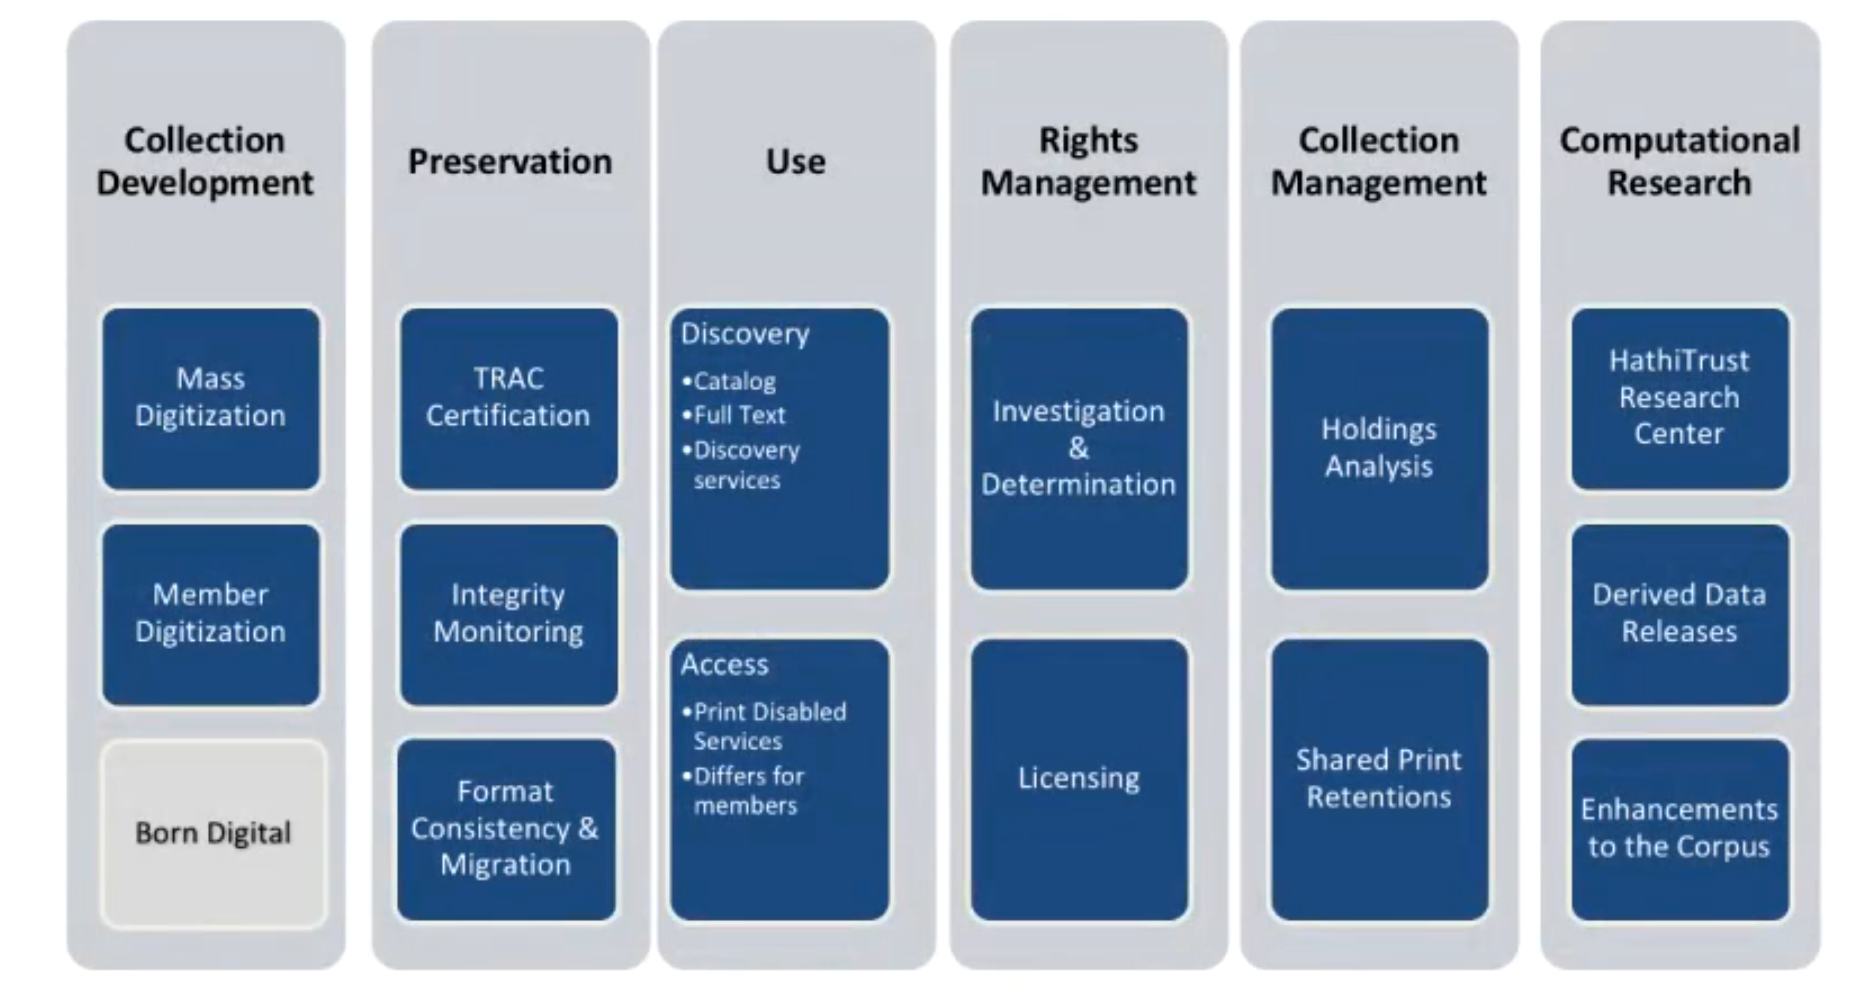
\includegraphics[width=15cm]{hathigoals}
\caption{Résumé des différentes activités entreprises par \textit{HathiTrust}, capture d'écran}
\end{figure}

La plateforme, inaugurée en 2008, propose des livres, articles de journaux sous licences ou libres de droit. Voulue indépendante du projet de Google, elle intègre également de nombreuses autres collections découlant de divers projets de numérisation de masse, publics (\textit{Internet Archive}) ou privés (\textit{Microsoft}). \textit{HathiTrust} regroupe plus d'une centaine de bibliothèques partenaires (140) à travers le monde\footcite{obrien_large-scale_2015} et offre un accès à quelques \textbf{seize millions} de documents\footcite{xie_discover_2016}\footcite{hathitrust_digital_library_charting_nodate}. Active dans différents domaines, l'organisation contribue notamment à la poursuite des projets de numérisation au sein des institutions partenaires en permettant le partage des coûts, et à accroître l'accessibilité et l'usage pour la recherche des données préservées. À travers le développement de différents outils et la mise en place du centre pour les recherches analytiques de \textit{the HathiTrust Research Center Analytics}, l'initiative soutient les travaux de recherches d'envergure conduits dans un objectif scientifique et par des organisations à but non lucratifs\footcite{hathitrust_digital_library_htrc_nodate}.

Pour regrouper les collections des différents partenaires et répondre aux besoins d'interopérabilité, un groupe collaboratif a développé un modèle de gestion des métadonnées visant à regrouper les différentes données des institutions et à en permettre l'exportation dans le format du projet : \textit{Zephir}\footcite{hathitrust_digital_library_zephir_nodate}. Portée par l'expertise des bibliothèques partenaires, la recherche offre des fonctionnalités similaires à celles que l'on peut trouver via les interfaces de ces institutions, permettant de rechercher dans les index (titre, auteur etc.), en plus de la recherche avancée et d'une recherche plein-texte. De la qualité de ses métadonnées, découle la robustesse et les performances de son moteur de recherche\footcite{weiss_using_2014}. L'affichage des résultats est toutefois limité en fonction du droit d'auteur\footcite{lau-suchet_hathitrust_2014}, puisque \textit{HathiTrust} vise avant tout à préserver les collections et s'inscrit moins dans une démarche d'accessibilité universelle. Certains ouvrages soumis au droit d'auteur ne peuvent être recherchés ou certaines fonctionnalités de la plateforme sont réservées aux membres des institutions partenaires (comme le téléchargement pdf des textes libres de droit), ce qui a valu au projet quelques critiques\footcite{wu_building_2011}\footcite{obrien_large-scale_2015}\footcite{xie_discover_2016}. 

L'anglais représente la langue majoritaire dans les collections\footcite{weiss_using_2014}, même si l'initiative poursuit l'objectif de permettre la recherche dans tous les systèmes d'écriture existants (actuellement celle-ci est disponible en caractères cyrilliques, hébreux, grecs, chinois, japonais et coréens)\footcite{lau-suchet_hathitrust_2014}.
\newpage
\begin{figure}[H]% force à placer l'image au sein de notre balise figure
\centering
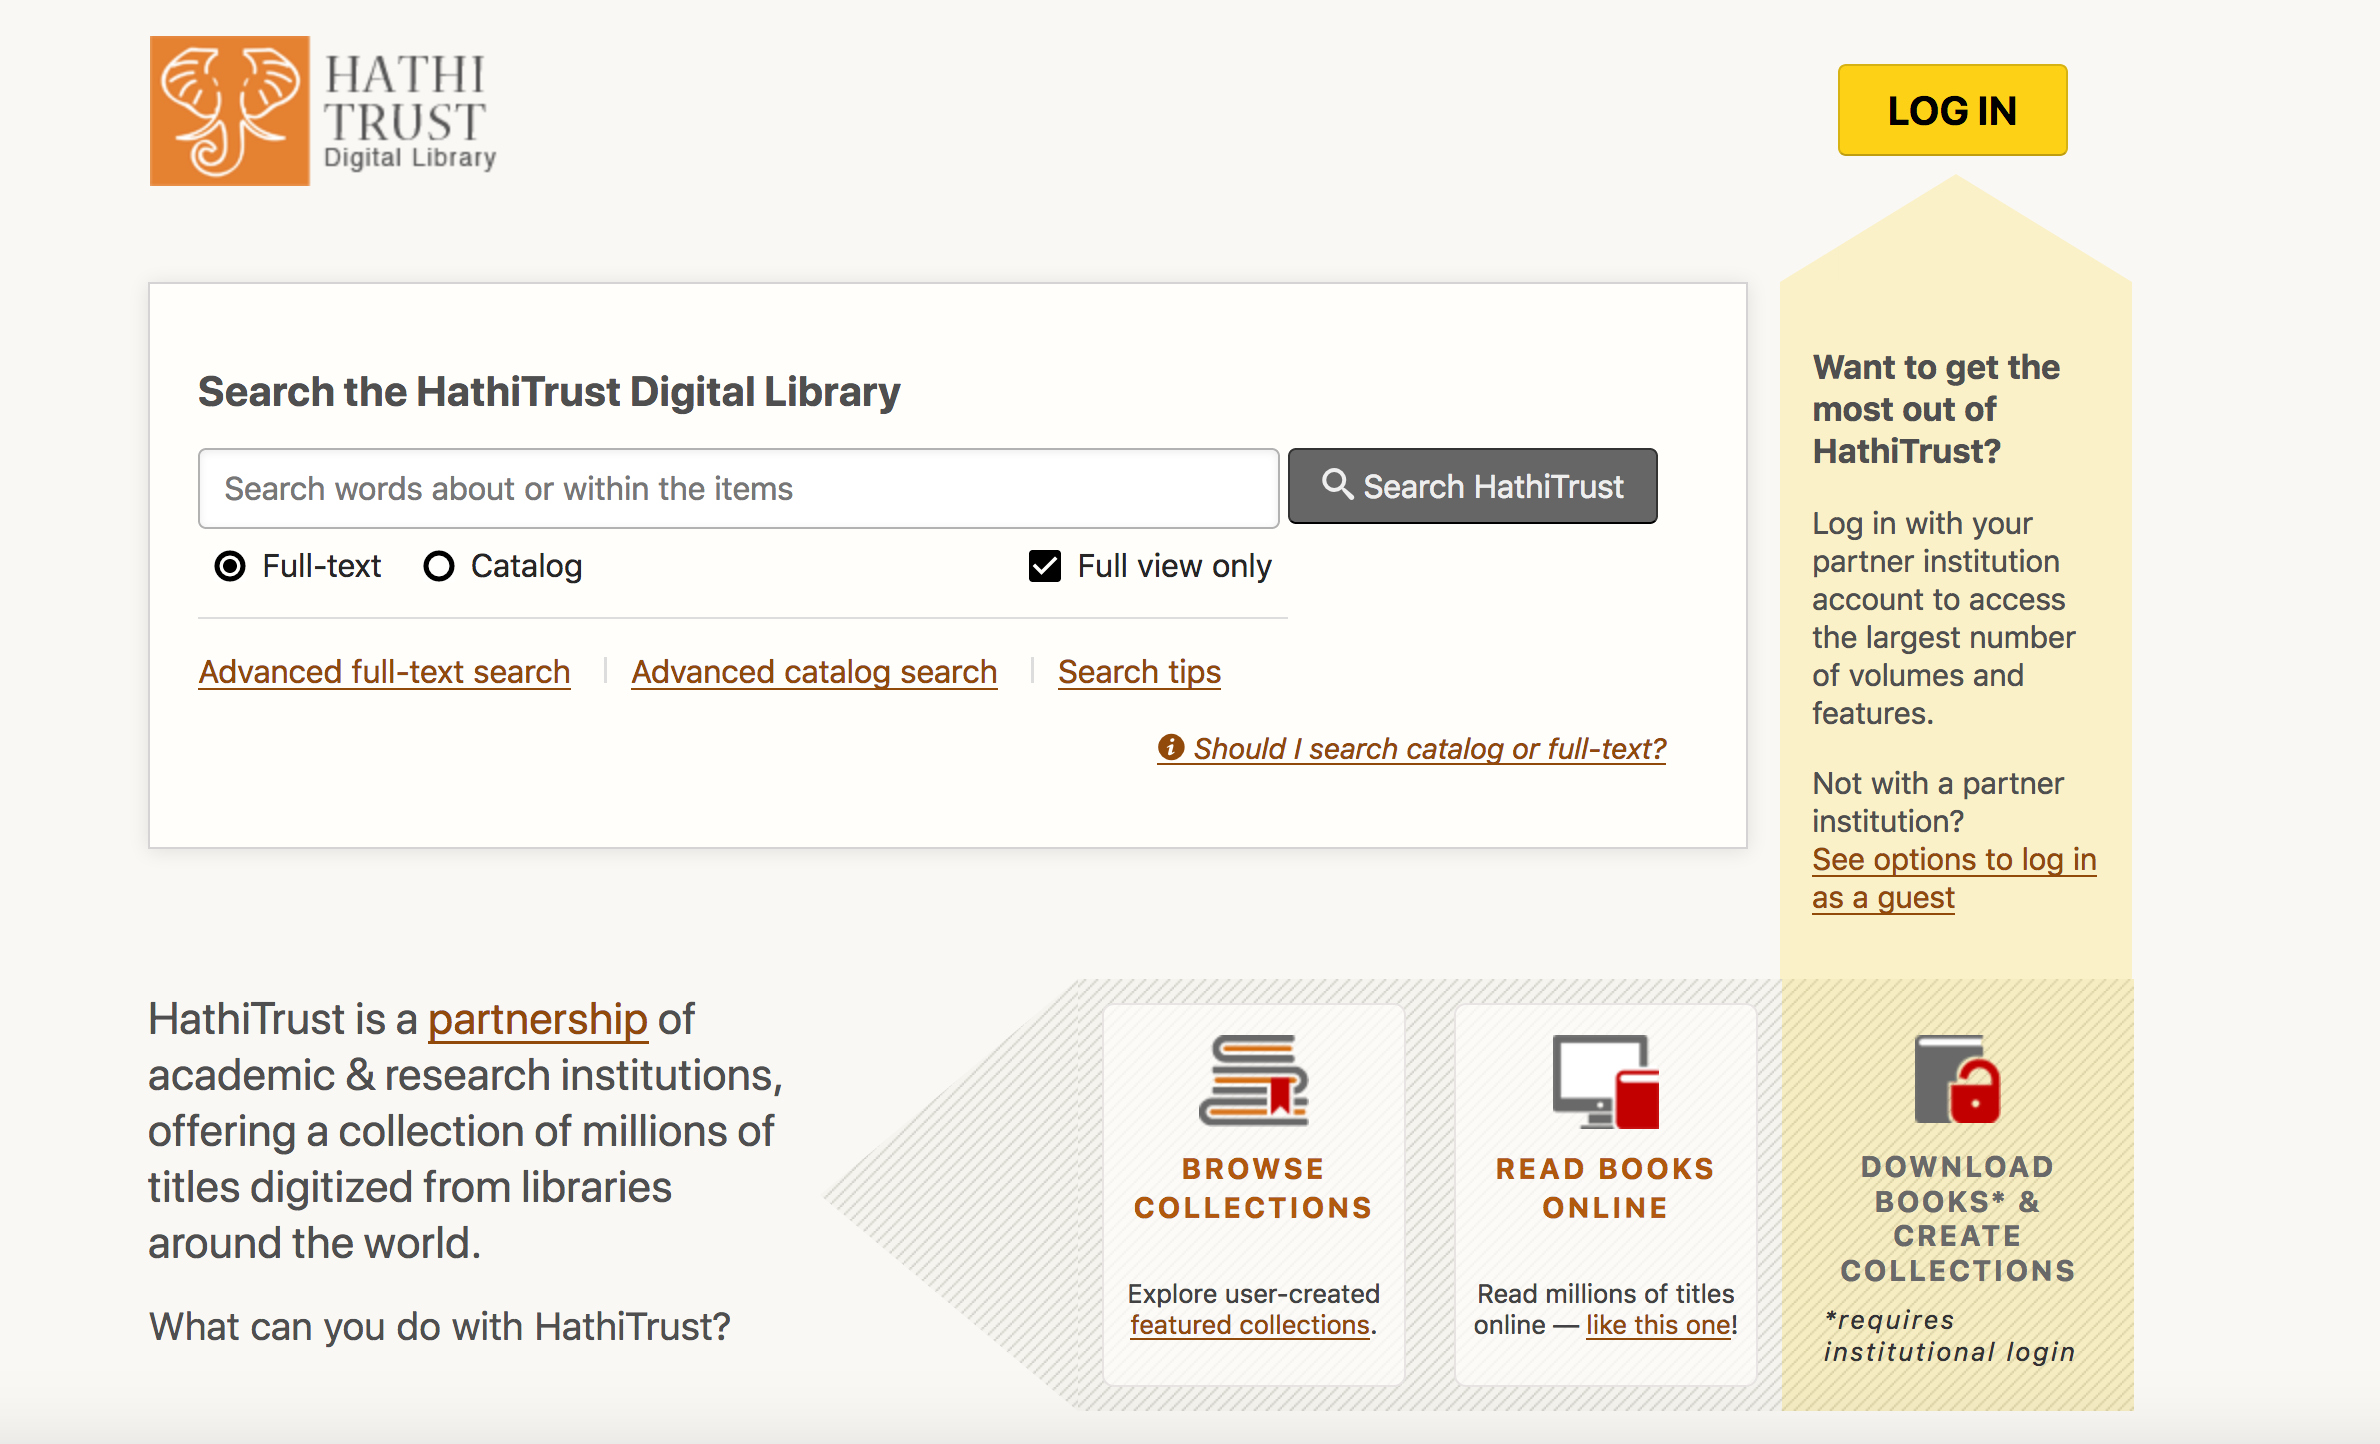
\includegraphics[width=15cm]{hathiface}
\caption{Page d'accueil de la plateforme d'\textit{HathiTrust}, capture d'écran}
\end{figure}

À l'inverse de Google, \textit{HathiTrust} sait gérer les ouvrages en plusieurs volumes, ce qui contribue à leurs découvertes\footcite{weiss_examining_2016} et s'attèle à vérifier le statut d'un document lorsque des doutes liés au droit d'auteur persistent\footcite{weiss_examining_2016}. La collaboration entre institutions partenaires est réalisée dans la plus grande transparence, et le site internet, mis à jour régulièrement, offre les derniers détails sur les décisions stratégiques soumises à l'approbation générale (dont les directions stratégiques envisagées pour la période 2019-2023)\footcite{hathitrust_digital_library_charting_nodate}. \textit{HathiTrust} développe des interfaces spécialement destinées aux personnes en situation de handicap\footcite{hathitrust_digital_library_charting_nodate}, ce qui contribue à accroître l'accessibilité de ses collections.
\newpage
\begin{table}[H]
\centering
\begin{tabular}{|l|l|}
\hline
\rowcolor[HTML]{2E1A46} 
{\color[HTML]{FFFFFF} \textbf{Enjeux}}                                                                                   & {\color[HTML]{FFFFFF} \textbf{Réponses de HathiTrust}}                                                                                                                                                                                                                                                                                                                                                                                                                                                                                                                                         \\ \hline
{\color[HTML]{2E1A46} \textbf{\begin{tabular}[c]{@{}l@{}}Amener différents\\ acteurs à collaborer\end{tabular}}}         & \begin{tabular}[c]{@{}l@{}}Projet collaboratif, porté par quelques 140 \\ bibliothèques partenaires. Une complète transparence\\ semble être garante d'une cohésion d'ensemble.\end{tabular}                                                                                                                                                                                                                                                                                                                                                                                                   \\ \hline
{\color[HTML]{2E1A46} \textbf{\begin{tabular}[c]{@{}l@{}}Financement et \\ partenariats \\ public-privé\end{tabular}}} & \begin{tabular}[c]{@{}l@{}}Les bibliothèques financent les infrastructures, selon une \\ somme calculée sur différents facteurs à la fois liés aux \\ collections de l'institution mais également à la taille du \\ réseau et au pourcentage d'\oe{}uvres sous droits. Le projet \\ ne semble pas recourir à des financements privés, mais\\ bénéficie de leurs entreprises de numérisation.\end{tabular}                                                                                                                                                                                          \\ \hline
{\color[HTML]{2E1A46} \textbf{Droit d'auteur}}                                                                           & \begin{tabular}[c]{@{}l@{}}HathiTrust a gagné son procès contre la guilde \\ des auteurs aux États-Unis. Il limite l'accès plein-texte des\\ ouvrages sous droits et entreprend de véritables recherches\\ afin de déterminer si des licences s'appliquent.\end{tabular}                                                                                                                                                                                                                                                                                                                       \\ \hline
{\color[HTML]{2E1A46} \textbf{\begin{tabular}[c]{@{}l@{}}Sortir des silos : \\ enjeux techniques\end{tabular}}}          & \begin{tabular}[c]{@{}l@{}}La qualité des métadonnées caractérisent le projet, favorisant\\ l'efficacité du moteur de recherche. Un système de gestion\\ dédié a été développé : \textit{Zephir}. Ce dernier attribue un score\\ à chaque fichier de métadonnées en fonction des informations\\ trouvées dans les différents champs de métadonnées. Si ce \\ score est trop bas, l'institution sera priée de corriger les \\ éléments manquants ou une notice développée par un autre\\ partenaire sera utilisée. Différentes APIs favorisent l'accès \\ aux métadonnées ou aux documents.\end{tabular} \\ \hline
{\color[HTML]{2E1A46} \textbf{\begin{tabular}[c]{@{}l@{}}Sortir des silos : \\ enjeux sur le \\ contenu\end{tabular}}}   & \begin{tabular}[c]{@{}l@{}}Le projet est motivé par des besoins académiques et ses\\ collections portent de fait le même biais scientifique que\\ les institutions partenaires. On observe une plus\\ forte représentation des ouvrages en langue anglaise. \\ Très peu d'institutions sont partenaires en dehors de\\ ce milieu linguistique. Les formats des collections sont \\ limités aux livres et articles de presse. Le projet rassemblant \\ des données préalablement numérisées, ses collections \\ offrent une forte redondance avec celles d'autres initiatives.\end{tabular}     \\ \hline
{\color[HTML]{2E1A46} \textbf{\begin{tabular}[c]{@{}l@{}}Stockage sur le \\ long-terme - \\ préservation\end{tabular}}}  & \begin{tabular}[c]{@{}l@{}}Le point fort du projet. L'infrastructure a été conçue pour \\ garantir la longévité des données et suit les normes récentes. \\ Les métadonnées de provenance et de contexte, et l'intégrité\\ et l'authenticité des documents sont préservés.\end{tabular}                                                                                                                                                                                                                                                                                                        \\ \hline
\end{tabular}
\caption{Les réponses de \textit{HathiTrust} aux enjeux de la numérisation}
\end{table}

\section{Agréger pour mieux valoriser}

%==== Europeana

\subsection{Europeana}

Issue de diverses réactions politiques à l'arrivée de \textit{Google Books}\footnote{En 2004, le Président français Jacques Chirac demande au directeur de la BNF Jean-Noël Jeanneney de lancer un projet européen similaire. Le directeur étant effrayé à la perspective de laisser les lois anglo-saxonnes s'imposer en Europe, il appelle à un effort national de numérisation et à la création d'une infrastructure européenne à même de préserver les différences culturelles des nations. Toutefois Europeana ne s'est pas construit comme une réponse à \inquote{l'invasion américaine}, d'autres voix plus pragmatiques, à l'instar de celle du président de la Commission européenne, José Manuel Barroso, ont argumenté du besoin de créer une économie de la connaissance \cite{thylstrup_politics_2018}}, Europeana est lancée par l'\gls{ue} en 2008, motivée par la perspective de créer une nouvelle économie de la connaissance. Le projet vise à favoriser le partage de contenus de qualités vers une audience européenne, à agrandir le nombre des partenaires afin de toucher toutes les parties concernées et à susciter l'intérêt du public quel qu'il soit, pour les contenus des institutions culturelles et patrimoniales\footcite{europeana_europeana_nodate-2}. La plateforme donne accès à quelques \textbf{58 millions} d'objets numérisés et élargit le spectre de leurs typologies. Les collections multilingues se composent d'images (33.5 millions), de textes (22.8 millions), de fichiers audio (700'000) ou vidéo (1.2 millions) et d'objets 3D (28'000) issus de plus de 3500 institutions\footcite{europeana_europeana_nodate-2}\footcite{xie_discover_2016}\footcite{noauthor_european_2019}.

En temps qu'\gls{agr}, Europeana bénéficie des entreprises de numérisations menées à l'échelle d'une nation ou d'une région, faisant converger les attentes de chacun au sein d'une infrastructure commune : \inquote{\textit{Europeana produces a new form of cultural memory politics that converge national and supranational imaginaries with global information infrastructures}\footcite[p.57]{thylstrup_politics_2018}}.
\newpage
\begin{figure}[H]% force à placer l'image au sein de notre balise figure
\centering
\includegraphics[scale=0.3]{europeana}
\caption{Page d'accueil de l'interface découverte d'Europeana, capture d'écran}
\end{figure}

Bien que se réclamant d'une souveraineté nationale, Europeana travaille avec les grands réseaux du web (Google, Microsoft etc.) pour financer la numérisation des données qui seront rassemblées sur sa plateforme. Présenté comme une initiative européenne, le projet réagit à des règles de privatisation induites par ces partenariats\footcite{thelle_persuasive_2011}. Les frontières entre public-privé tendant à se moduler à travers l'infrastructure, et celles entre institutions et environnement suivent la même logique\footcite[p.63]{thylstrup_politics_2018}. Ce paradoxe sera d'ailleurs souvent critiqué\footcite{thelle_persuasive_2011}\footcite{thelle_persuasive_2011}.

\begin{quotation}
[\textit{Traduction}]
Si Europeana est un projet de numérisation de masse construit autour d'anciennes logiques souveraines, dont le discours officiel valorise l'État nation, en même temps qu'il abolit les frontières en déployant des infrastructures interopérables, la question demeure : quel est le résultat de cet assemblage d'un point de vue culturel ?\footnote{\inquote{\textit{If Europeana is a late-sovereign mass digitization project that maintains discursive ties to the national imaginary at the same time that it undercuts this imaginary by means of networked infrastructure through increased interoperability, the final question is: what does this late-sovereign assemblage produce in cultural terms?}}\cite[p.73]{thylstrup_politics_2018}}
\end{quotation}

Europeana étant un projet sous financement européen, il respecte le droit d'auteur \footnote{par opposition à Google avec son application du \textit{fair use}}, alors même que ce système est très complexe à déployer. Comme l'Europe ne possède pas de législation commune, il navigue entre les différentes particularités nationales, l'émergence d'un marché global et la mouvance du \gls{oa}\footcite{thylstrup_politics_2018}\footcite{weiss_using_2014}. Europeana favorise les contenus en accès libres sous licence \textit{\gls{cc}} CC0\footnote{Licence la moins restrictive, n'obligeant pas à citer la provenance du contenu.}, ce qui pose des problèmes d'application pour certains États (dont la France), plus restrictifs\footcite{noauthor_european_2019}. On retrouve également différentes formes d'affichage en fonction de ces restrictions (accès aux contenus interactifs et aux métadonnées, accès aux contenus statiques et métadonnées, extraits et métadonnées, métadonnées seulement)\footcite{willems_europeana_2015}. Les \oe{}uvres à partir du 20\up{e} siècle sont sous-représentées au profit des \oe{}uvres libres de droit\footcite{dufrene_numerisation_2013}\footcite{stobo_i_2018}.

Pour tenter de répondre à ces différentes contraintes tout en effectuant sa mission, Europeana investit le principe d'interopérabilité : proposant notamment un cadre de publication à destination des institutions directement ou des \gls{agr}s nationaux et thématiques de collections numérisées\footnote{Afin de mieux interagir avec les plateformes et institutions existantes, Europeana a créé en 2012 le \textit{Europeana Aggregator forum}. Ce lieu permet la mise en place d'échanges professionnels et assure l'implication de ces instances stratégiques au sein du projet. Les agrégateurs offrent à leurs institutions partenaires conseils et support dans leurs projets de numérisation concernant le choix les licences ; formats ;  traitement du multilinguisme etc... \cite{europeana_breathing_nodate}. Plus de 2/3 des États membres ont des agrégateurs nationaux \cite{noauthor_european_2019}.} ; une stratégie de contenu ; un modèle de métadonnées suivant les recommandations du web sémantique\footcite{europeana_linked_nodate-1} et proposant un enrichissement à l'aide de vocabulaires contrôlés\footnote{Lexique servant à organiser les connaissances pour favoriser la recherche d'information} ;  des modèles de licences basés sur les \textit{\gls{cc}}. Plusieurs \gls{api}s (dont celles développées par \gls{iiif}) contribuent à l'accessibilité des collections et la naissance de nouveaux produits\footcite{roued-cunliffe_participatory_2017}\footnote{à l'instar de l'\textit{EuropeanaBot}, garant d'une certaine forme de sérendipité, puisque publiant aléatoirement des images issues des collections. \cite{noauthor_europeana_nodate}.}. Les données sont également rendues accessibles via le protocole \gls{oai}\footcite{europeana_everything_nodate}. Soucieuse de garantir une meilleure utilisation des données, Europeana conjointement avec \gls{dpla} et d'autres institutions, fait partie du \textit{RightsStatements.org} Consortium proposant des \inquote{déclarations de droits standardisées pour le patrimoine culturel disponible en ligne}\footcite{noauthor_rightsstatements.org_nodate}. Les institutions peuvent choisir entre 12 déclarations (en cours de traductions dans tous les idiomes européens), favorisant l'usage des fichiers par le public\footcite{noauthor_european_2019}. 

De nombreuses communautés sont impliquées dans Europeana. Le projet s'est construit dans la mouvance des \gls{cs}, dès lors ces communautés participent entre autres aux corrections, transcriptions, classification, contextualisation des données numérisées. L'expérience promue par le projet est de ne pas simplement demander aux utilisateurs de cliquer, mais de leur offrir l'opportunité de prendre une part active dans un projet de recherche\footcite{thylstrup_politics_2018}. Ce souci d'impliquer l'utilisateur se retrouve dans le développement de la plateforme et des services, héritage probable des pratiques mises en place au sein des institutions partenaires\footcite{jones_public_2017}. 

Pour améliorer l'expérience utilisateur et lui permettre de trouver son chemin face aux collections foisonnantes, des expositions virtuelles ont été créées\footcite{europeana_europeana_nodate-2}, la recherche peut se faire dans toutes les langues européennes mais les métadonnées, proposées en résultat ne sont pas traduites\footcite{noauthor_european_2019}. Europeana propose deux interfaces différentes, s'adressant d'un côté à l'utilisateur \inquote{grand public} et mettant en avant la découverte, ou interagissant en toute transparence sur sa plateforme professionnelle avec les partenaires du réseau et les entités ou individus motivés à profiter pleinement des opportunités offertes par ses collections massives (éducation, recherche, industries etc.)\footcite{ioana_roiu_cristina_family_nodate}. L'interface professionnelle décrit précisément l'organisation, les spécificités techniques et propose des accompagnements ciblés selon si l'on se positionne en tant que partenaire du réseau, chercheur, ou futur exploitant\footcite{europeana_europeana_nodate-2}. 

Europeana propose depuis les débuts des interfaces mobiles, ce qui est important pour le projet, car la plupart de son trafic provient des portables\footcite{xie_discover_2016}.
 \newpage
\begin{figure}[H]% force à placer l'image au sein de notre balise figure
\centering
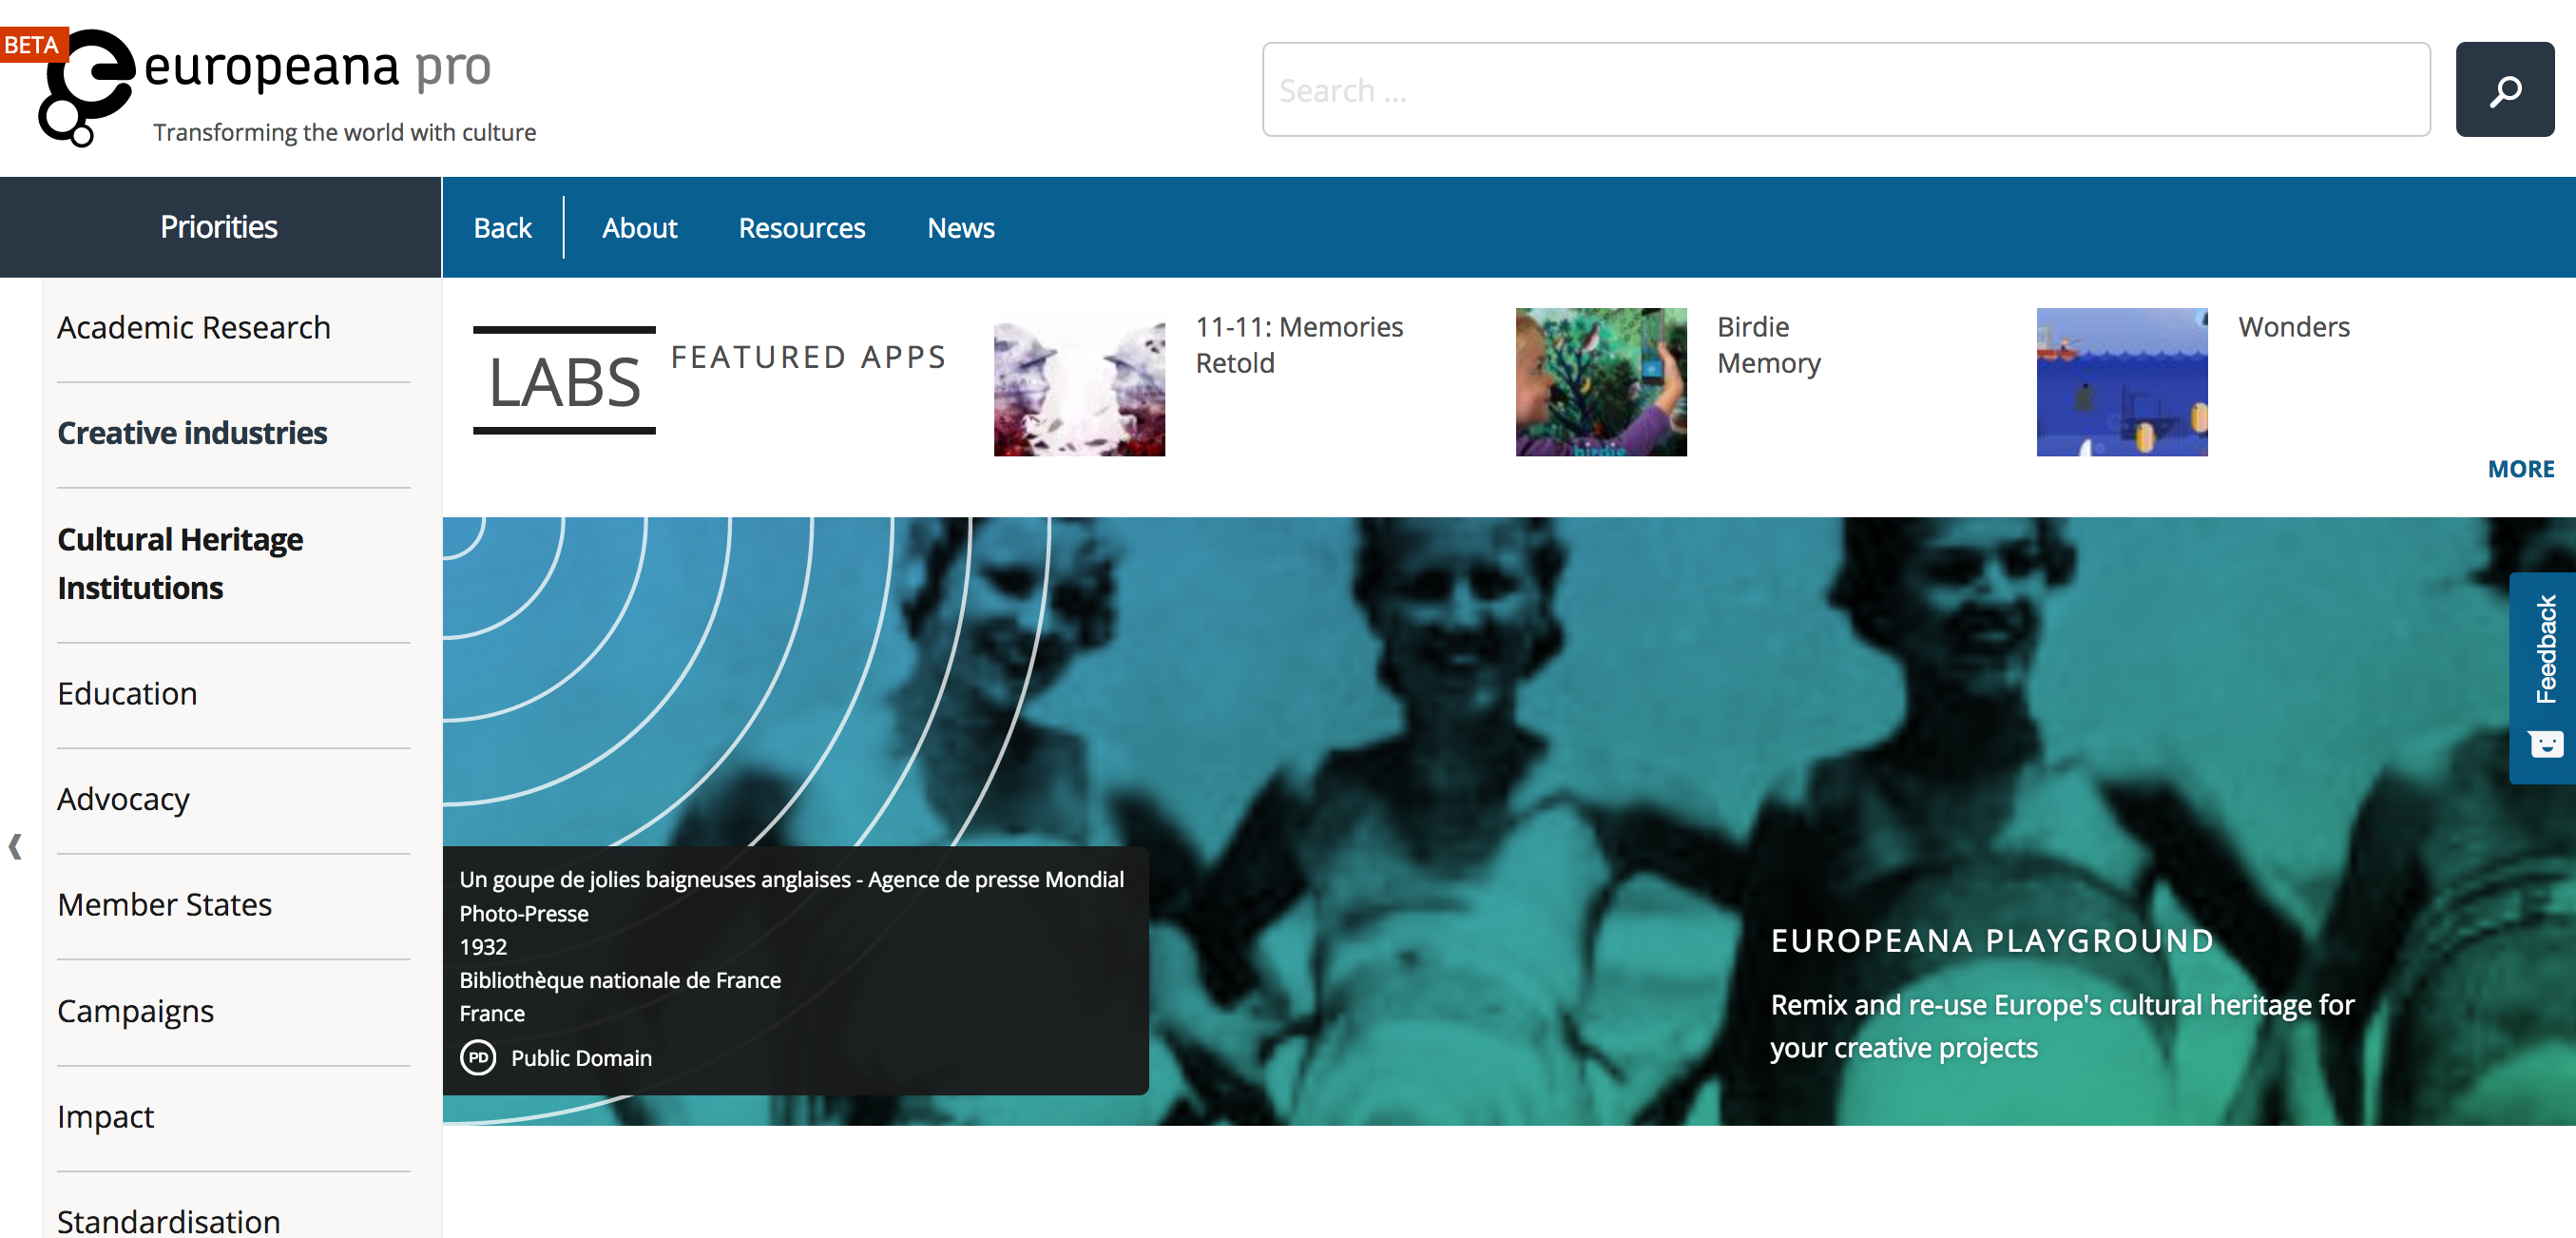
\includegraphics[width=15cm]{europeanapro}
\caption{Page d'accueil de l'interface professionnelle d'Europeana, capture d'écran}
\end{figure}

Se voulant reflet du patrimoine culturel européen, ses collections n'en sont toutefois pas pleinement représentatives. Certains pays ont moins développé la numérisation (biais géographique), certaines typologies d'objets sont sous-représentées, les collections héritent des biais des institutions partenaires\footcite{thylstrup_politics_2018}. Ce qui amènera un responsable d'Europeana à caractériser, en 2010, la différence entre Google et Europeana, par le fait que d'un côté l'usager accède à tout, alors que de l'autre les collections ont été soigneusement sélectionnées par les institutions en vue de leur numérisation\footcite{thelle_persuasive_2011}. Toutefois Europeana tente de proposer de nouvelles formes de numérisation, impliquant le citoyen dans le processus de sélection\footnote{Dans le cadre du projet Europeana 1914-1918, les individus ont été sollicités afin de créer une archive de la Première Guerre Mondiale basée sur leurs images et écrits familiaux \cite{ioana_roiu_cristina_family_nodate}.}, et a mis en place une stratégie de contenu visant à pallier aux manques des collections\footcite{europeana_everything_nodate}.

Europeana n'est pas responsable du stockage sur le long-terme des collections numérisées. Une forte disparité est constatée au niveau européen concernant l'existence de législations relatives à la préservation des données. Cette dernière est souvent dépendante du bon vouloir des institutions\footcite{noauthor_european_2019}.

Malgré son ancrage européen, Europeana est embranchée dans un écosystème Google, laissant le projet à la merci de changements de sa stratégie de référencement et par conséquent face au risque de perdre en visibilité\footcite{thylstrup_politics_2018}. Afin de mieux traiter la richesse des langues européennes, le projet a d'ailleurs intégré une fonction Google, \textit{Google Translate}\footcite{thelle_persuasive_2011}. Depuis 2011, les bibliothèques européennes signataires d'un accord de numérisation avec Google voient leurs documents indexés par Europeana\footcite{moatti_bibliotheque_2012}.

L'\gls{ue} a récemment fixé les nouvelles priorités pour Europeana, qui visent à : développer le multilinguisme de la plateforme ; améliorer la valorisation des collections et proposer de nouveaux services de découverte ; mieux prendre en compte les besoins des petites institutions\footcite{noauthor_european_2019}.

\newpage
\begin{table}[H]
\centering
\begin{tabular}{|l|l|}
\hline
\rowcolor[HTML]{2E1A46} 
{\color[HTML]{FFFFFF} \textbf{Enjeux}}                                                                                   & {\color[HTML]{FFFFFF} \textbf{Réponses d'Europeana}}                                                                                                                                                                                                                                                                                                                                                                                                                                                     \\ \hline
{\color[HTML]{2E1A46} \textbf{\begin{tabular}[c]{@{}l@{}}Amener différents\\ acteurs à collaborer\end{tabular}}}         & \begin{tabular}[c]{@{}l@{}}Une grande transparence et l'élaboration du cadre technique\\ en collaboration étroite avec les partenaires semblent être\\ garants d'une bonne collaboration. De nombreux groupes\\ de travail impliquant les institutions contribuent aux \\ évolutions du projet. Les agrégateurs nationaux ou thématiques\\ sont intégrés au sein d'un forum, favorisant les échanges. Le \\ grand public devient partenaire des projets de recherche.\end{tabular}                      \\ \hline
{\color[HTML]{2E1A46} \textbf{\begin{tabular}[c]{@{}l@{}}Financement et \\ partenariats \\ public-privé\end{tabular}}} & \begin{tabular}[c]{@{}l@{}}Comme la plupart des projets de numérisation sont\\ conduits de manière décentralisées par les institutions,\\ ces dernières se tournent vers des institutions\\ privées (Google, Microsoft etc.) pour les financer. \\ L'Europe finance l'infrastructure et quelques projets de \\ numérisation ciblés.\end{tabular}                                                                                                                                                         \\ \hline
{\color[HTML]{2E1A46} \textbf{Droit d'auteur}}                                                                           & \begin{tabular}[c]{@{}l@{}}Le projet agit dans la légalité et applique des licences\\ et restrictions aux \oe{}uvres sous droit.\\ Un cadre de publication règle les conditions d'échange\\ des métadonnées et s'assure que la mention de la licence \\ y figure. Les licences \textit{Creative Commons} sont privilégiées. \\ Membre du \textit{RightsStatements}, le projet propose des \\ déclarations de droit standardisées. Différentes formes \\ d'affichage garantissent un accès légal aux collections.\end{tabular} \\ \hline
{\color[HTML]{2E1A46} \textbf{\begin{tabular}[c]{@{}l@{}}Sortir des silos : \\ enjeux techniques\end{tabular}}}          & \begin{tabular}[c]{@{}l@{}}Un cadre de publication contenant un modèle de \\ métadonnées a été développé. Différentes APIs (dont IIIF) \\ sont déployées, le protocole OAI-PMH est disponible, les\\ métadonnées sont exposées suivant les principes du web\\ sémantique et enrichies grâce à des vocabulaires contrôlés.\end{tabular}                                                                                                                                                                   \\ \hline
{\color[HTML]{2E1A46} \textbf{\begin{tabular}[c]{@{}l@{}}Sortir des silos : \\ enjeux sur le \\ contenu\end{tabular}}}   & \begin{tabular}[c]{@{}l@{}}Conscient des biais liés aux formats, à la géographie et\\ à l'héritage des institutions partenaires, le projet a mis en \\ place une stratégie de contenu afin de pallier aux manques\\ constatés. De nombreux formats de documents sont disponibles,\\ dont des fichiers audio, vidéo et 3D. Les documents sont\\ multilingues mais le français est sur-représenté.\end{tabular}                                                                                            \\ \hline
{\color[HTML]{2E1A46} \textbf{\begin{tabular}[c]{@{}l@{}}Stockage sur le \\ long-terme - \\ préservation\end{tabular}}}  & \begin{tabular}[c]{@{}l@{}}Europeana n'a pas vocation à stocker directement les données,\\ (cette responsabilité est laissée aux institutions) \\ toutefois les critères de qualité imposés aux métadonnées \\ contribuent à la préservation de l'authenticité et \\ de l'intégrité des documents.\end{tabular}                                                                                                                                                                                              \\ \hline
\end{tabular}
\caption {Les réponses d'Europeana aux enjeux de la numérisation}
\end{table}

 
\subsection{Digital Public Library of America}

La \textit{Digital Public Library of America} ou \gls{dpla}, pensée dès 2010 et officiellement lancée en 2013 vise à rendre le contenu des institutions culturelles et patrimoniales états-uniennes accessible à tous. Deux programmes ont été mis en place pour répondre à cette mission : l'agrégation des données numériques des institutions de tous les États-Unis et un service d'ebooks\footcite{digital_public_library_of_america_strategic_nodate}\footcite{digital_public_library_of_america_history_nodate}. Ce projet est en grande partie dû aux travaux intellectuels du \textit{Berkman Klein Center for Internet and Society\footnote{La mission de ce centre est notamment d'explorer le cyberespace et d'identifier le besoin de nouvelles législations ou des ajustements de celles existantes.}} de l'université d'Harvard et de grands théoriciens du numérique, et des bibliothèques, qui ont travaillé à le positionner comme une alternative publique à l'infrastructure privée de \textit{Google Books}\footcite{thylstrup_politics_2018}. Cependant, comme dans toutes les initiatives de numérisation de masse, la notion de \inquote{public} suscite de nombreuses controverses, puisque l'on reproche à ces projets de détourner l'argent autrement réservé aux infrastructures plus petites\footcite{thylstrup_politics_2018}. 

Le réseau rassemble quelques 41 États, plus de 4000 institutions et permet de découvrir à travers sa plateforme plus de \textbf{30 millions} d'objets de différentes typologies (images, cartes, fichiers audio, manuscrits, \oe{}uvres muséales etc.)\footcite{digital_public_library_of_america_strategic_nodate}. Au même titre qu'Europeana, le projet n'héberge pas ces données, mais offre un portail permettant d'y accéder\footcite{pomerantz_metadata_2015}\footcite{xie_discover_2016}.

\begin{figure}[H]% force à placer l'image au sein de notre balise figure
\centering
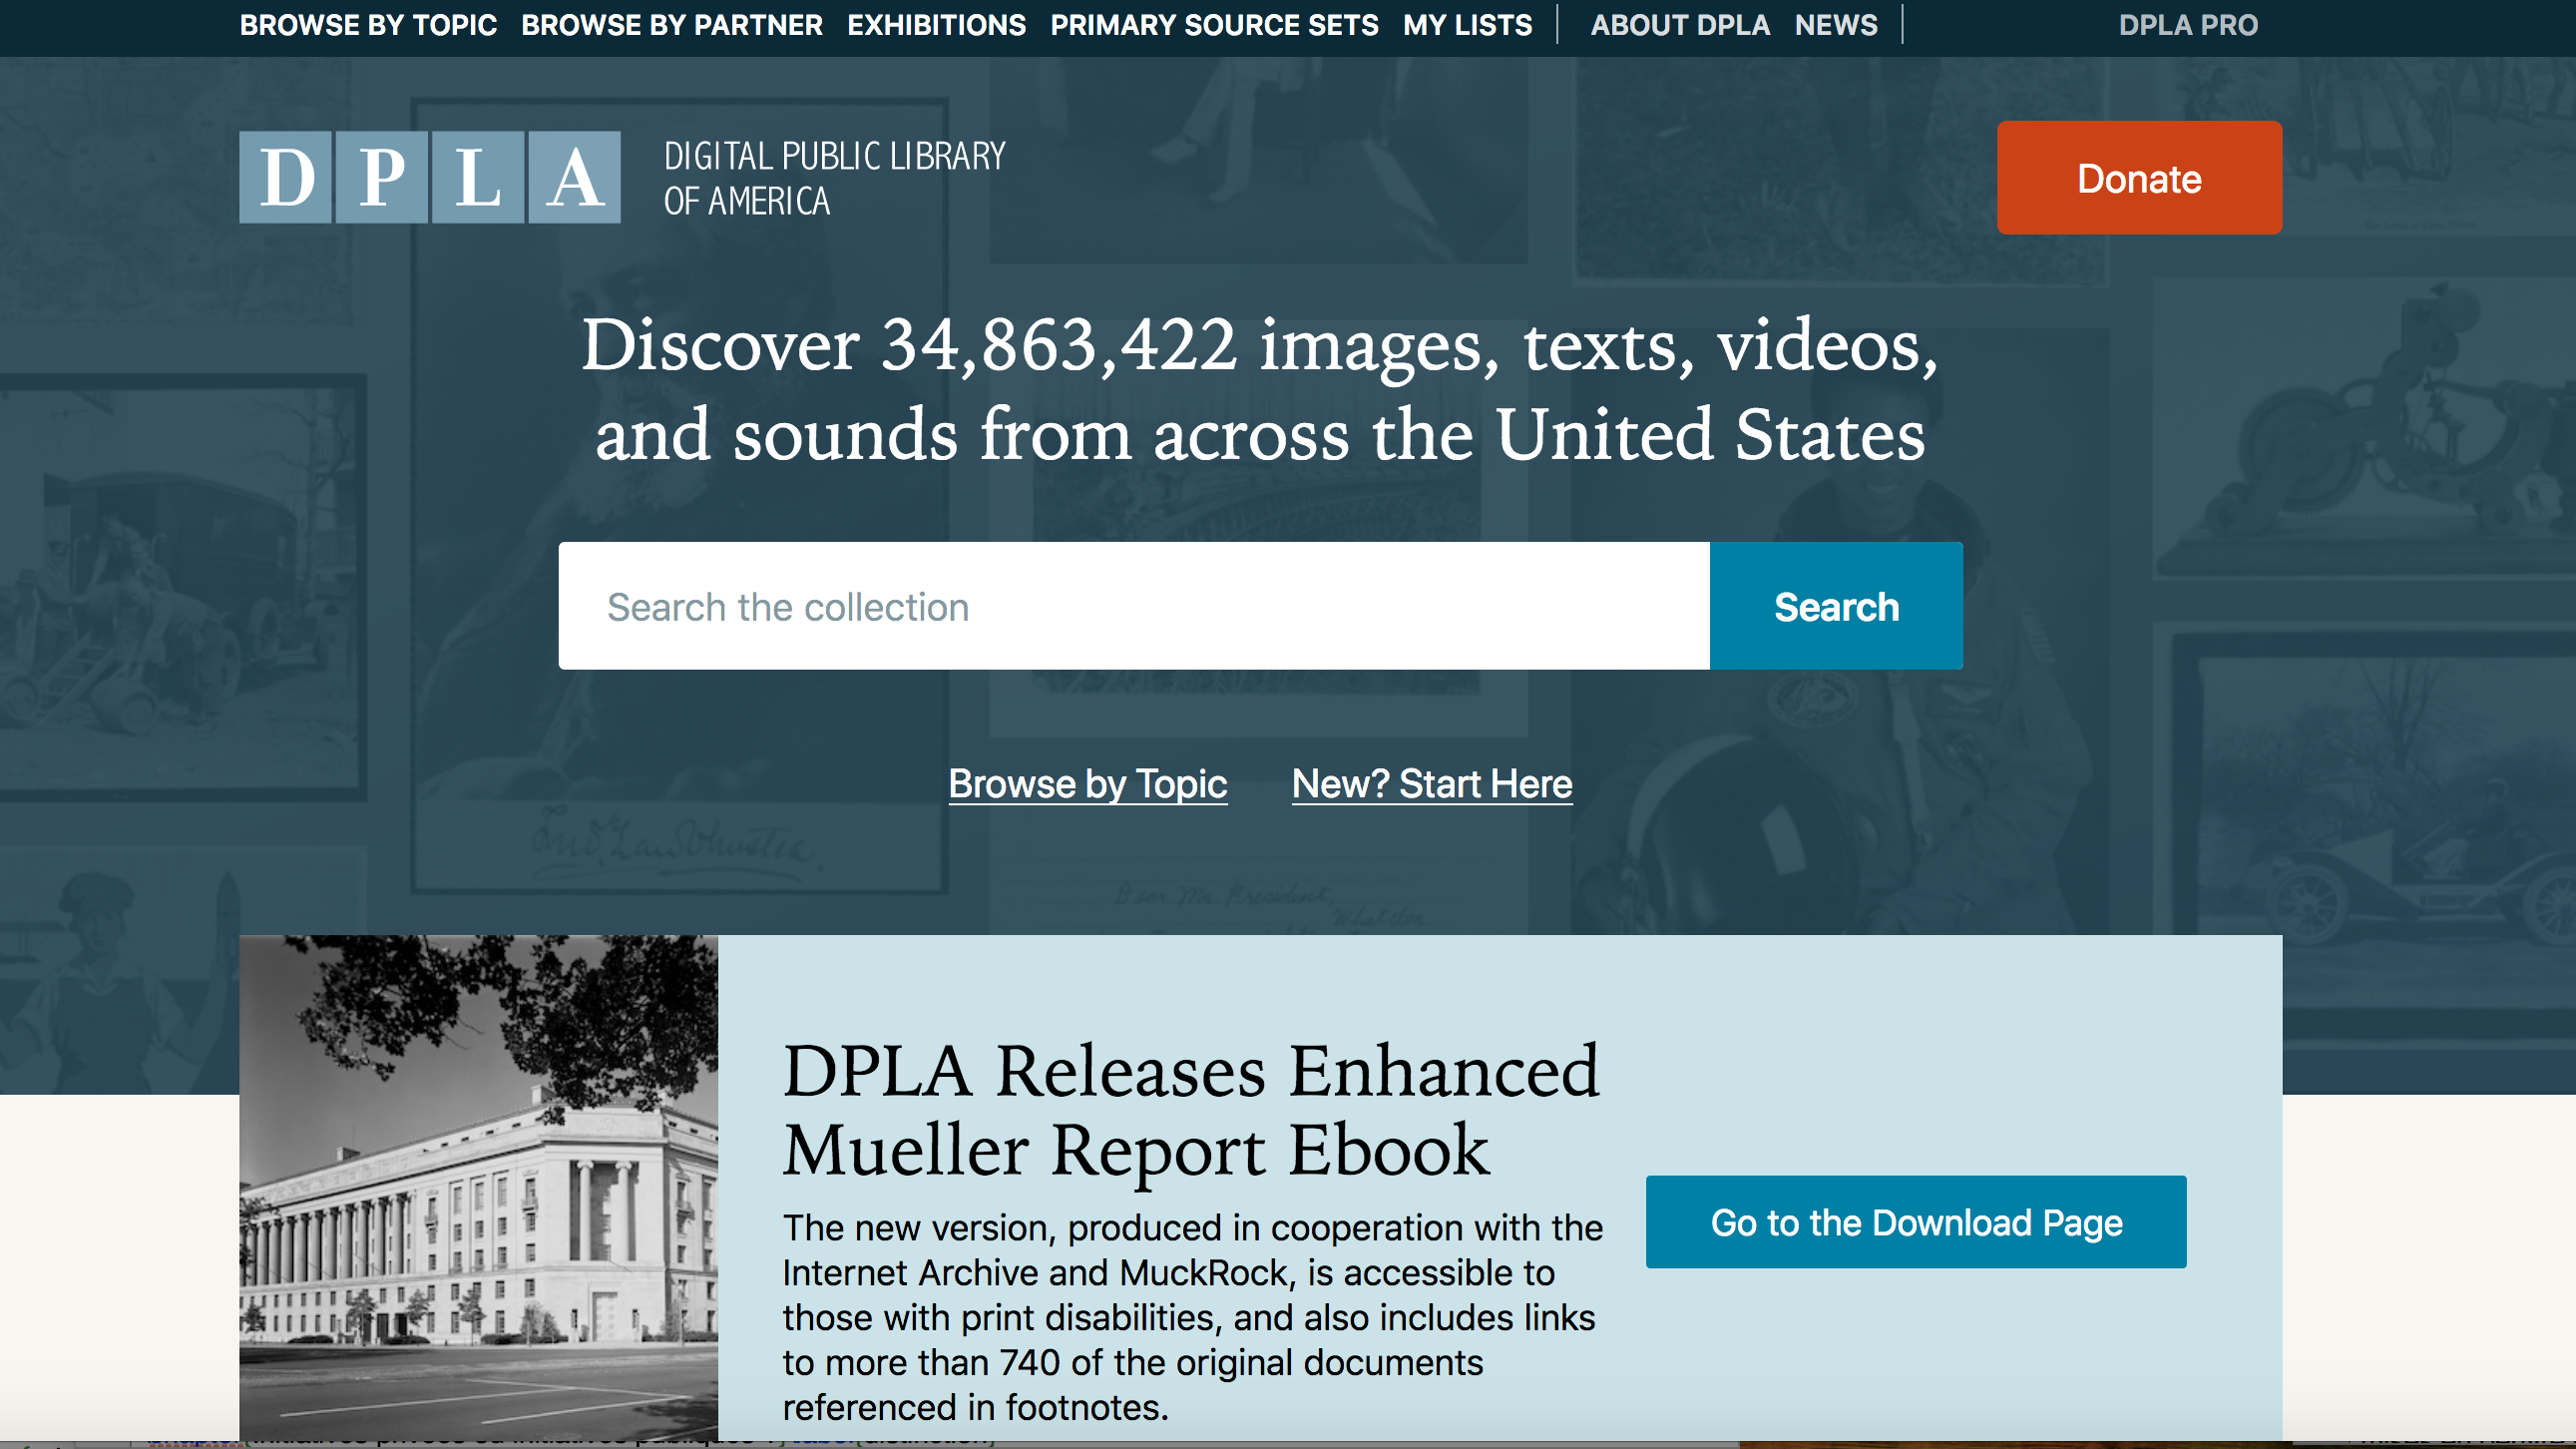
\includegraphics[width=15cm]{dpla}
\caption{Page d'accueil de l'interface découverte du projet de \gls{dpla}, capture d'écran}
\end{figure}

Bien que sa structure soit uniquement basée aux États-Unis, \gls{dpla} a été développé pour être interopérable avec Europeana (le même modèle de métadonnées est utilisé\footcite{digital_public_library_of_america_metadata_nodate}, les deux institutions collaborent au sein du \textit{RightsStatements.org} Consortium etc.). Les liens entre les deux initiatives contribuent ainsi à la création d'un réseau mondial\footcite{xie_discover_2016} et les placent à l'avant-garde d'un mouvement grandissant, visant à proposer des modèles de métadonnées spécifiques à certains domaines\footcite{pomerantz_metadata_2015}. \gls{dpla} s'appuie également sur un réseau d'\gls{agr}s nationaux qui facilitent l'intégration des données de leurs membres, et proposent des solutions de stockage pour les petites institutions qui n'en disposeraient pas\footcite{digital_public_library_of_america_becoming_nodate}\footcite{xie_discover_2016}. Des \gls{api}s permettent des requêtes sur le contenu et les métadonnées, la plateforme propose également un export total de ses \gls{db}\footcite{xie_discover_2016}.

L'initiative soutient une gestion des risques et l'application du \textit{fair use}, offerte par son ancrage géographique, pour justifier la numérisation des \oe{}uvres orphelines ou dont le libre accès suscite des doutes. Il incite toutefois les institutions à entreprendre des recherches sérieuses afin de déterminer si un contenu est libre de droit ou non, et offre un accompagnement dans cette démarche à ses partenaires\footcite{digital_public_library_of_america_understanding_nodate}. 

\gls{dpla} travaille au développement et à la mise en place de solutions techniques afin de soutenir l'engagement des communautés, la recherche et l'éducation. Ses missions actuelles s'articulent autour de différents projets visant à : favoriser l'usage des ebooks par le grand public et les bibliothèques ; accroître l'emploi des collections par le système éducatif ; clarifier l'usage des \oe{}uvres sous droit ; construire des solutions de dépôt numérique ; améliorer la présence de journaux issus de communautés marginalisées ; former les nouveaux partenaires aux technologies de la plateforme et les soutenir dans leurs entreprises de numérisation\footcite{digital_public_library_of_america_projects_nodate}. 

Tout comme Europeana, l'initiative dispose de deux plateformes, l'une permettant la découverte des collections et la deuxième, professionnelle, s'adressant plus précisément : aux agrégateurs partenaires ; aux candidats à la création d'un nouvel agrégateur ; aux communautés de développeurs ; aux chercheurs ; aux utilisateurs d'ebooks ; aux communautés de volontaires souhaitant promouvoir le projet \footcite{digital_public_library_of_america_our_nodate}. Soucieuse de faciliter l'accès à ses collections, la plateforme publique propose également des expositions virtuelles et a développé un \textit{Bot}\footnote{Programme autonome capable d'interagir avec un système ou un utilisateur.} afin de ramener la notion de sérendipité dans la découverte\footcite{thylstrup_politics_2018}.

 \begin{figure}[H]% force à placer l'image au sein de notre balise figure
\centering

\includegraphics[width=15cm]{dplapro}
\caption{Page d'accueil de l'interface professionnelle du projet de \gls{dpla}, capture d'écran}
\end{figure}

Ces projets et l'infrastructure sont financés par des fondations à but non lucratif, par des fonds du gouvernement américain et par une redevance prélevée auprès des institutions partenaires (qui varie entre 10'000 et 15'000 USD par an)\footcite{digital_public_library_of_america_membership_nodate}. Les institutions doivent elles-mêmes assurer les fonds nécessaires à la numérisation de leurs données mais peuvent être aidées dans cette recherche\footcite{digital_public_library_of_america_our_nodate-1}. Le projet indexe également des données numérisées par Google et stockées par \textit{HathiTrust}.

La collaboration fait partie intégrante de sa démarche, de nombreux groupes de travail sont mis en place afin de réfléchir aux développements de nouvelles solutions. Loin d'être partenaire du clivage Amérique - Europe, l'institution chercher à collaborer avec les réseaux existants\footcite{digital_public_library_of_america_our_nodate}. 
\newpage
\begin{table}[H]
\centering
\begin{tabular}{|l|l|}
\hline
\rowcolor[HTML]{2E1A46} 
{\color[HTML]{FFFFFF} \textbf{Enjeux}}                                                                                   & {\color[HTML]{FFFFFF} \textbf{Réponses de the Digital Public Library of America}}                                                                                                                                                                                                                                                                                                              \\ \hline
{\color[HTML]{2E1A46} \textbf{\begin{tabular}[c]{@{}l@{}}Amener différents\\ acteurs à collaborer\end{tabular}}}         & \begin{tabular}[c]{@{}l@{}}Collaborer fait partie des missions du projet. Une \\ plateforme professionnelle garantit la transparence de la\\ gouvernance. Différents groupes de travail permettent aux \\ partenaires de participer aux développements futurs. Les \\ communautés professionnelles, ou non, sont impliquées dans \\ le projet.\end{tabular}                                    \\ \hline
{\color[HTML]{2E1A46} \textbf{\begin{tabular}[c]{@{}l@{}}Financement et \\ partenariats \\ public-privé\end{tabular}}} & \begin{tabular}[c]{@{}l@{}}Le financement est assuré par le gouvernement américain, \\ des fondations à but non lucratif et une redevance versée\\ annuellement par les partenaires. Les projets de numérisation\\ sont à la charge des partenaires qui peuvent collaborer avec \\ des groupes privés (tels Google, Microsoft etc.).\end{tabular}                                              \\ \hline
{\color[HTML]{2E1A46} \textbf{Droit d'auteur}}                                                                           & \begin{tabular}[c]{@{}l@{}}Favorable à l'usage des licences \textit{Creative Commons}, encourage les \\ partenaires à tirer parti du \textit{fair use} et à mettre en place une gestion \\ des risques. Membre du \textit{RightsStatements}, le projet propose des\\ déclarations de droit standardisées.\end{tabular}                                                                                                  \\ \hline
{\color[HTML]{2E1A46} \textbf{\begin{tabular}[c]{@{}l@{}}Sortir des silos : \\ enjeux techniques\end{tabular}}}          & \begin{tabular}[c]{@{}l@{}}Adoption du modèle de métadonnées développé par \\ Europeana et interopérabilité avec sa plateforme. \\ APIs pour accéder aux métadonnées ou aux contenus.\end{tabular}                                                                                                                                                                                             \\ \hline
{\color[HTML]{2E1A46} \textbf{\begin{tabular}[c]{@{}l@{}}Sortir des silos : \\ enjeux sur le \\ contenu\end{tabular}}}   & \begin{tabular}[c]{@{}l@{}}Hérite des biais des institutions partenaires et sur-représentation de \\ certains formats de documents (textes et images). Un effort est fait \\ pour identifier les manques des collections et les corriger par la mise en \\ place de projets de numérisation ciblés.\end{tabular}                                                                               \\ \hline
{\color[HTML]{2E1A46} \textbf{\begin{tabular}[c]{@{}l@{}}Stockage sur le \\ long-terme - \\ préservation\end{tabular}}}  & \begin{tabular}[c]{@{}l@{}}Développe des solutions de dépôts institutionnels pour les petites\\ institutions et favorise les agrégateurs qui en proposent à leurs \\ communautés. Le stockage des données sur le long-terme demeure\\ sous la responsabilité des institutions. La qualité des métadonnées\\ favorisent le respect de l'intégrité et de l'authenticité des objets.\end{tabular} \\ \hline
\end{tabular}\caption {Les réponses de la \textit{Digital Public Library of America} aux enjeux de la numérisation}
\end{table}
\newpage

% Initiatives publiques versus initiatives privées
\chapter{Comment catégoriser ?}\label{distinction}

La comparaison plus détaillée de ces quatre initiatives de numérisation de masse permet de nuancer les propos de ceux qui distinguent initiatives financées par des institutions commerciales de celles financées par des institutions publiques ou à but non lucratif, puisque les activités de ces deux typologies de projet semblent étroitement imbriquées. Nous appuyons la réflexion contenue dans cette section sur les réponses apportées aux enjeux de la numérisation, bien que d'autres critères non étudiés dans le cadre de ce mémoire auraient pu servir à cette comparaison (tels que le rôle joué par l'homme au sein de ces projets, le nombre de publications officielles proposées etc...)\footcite{leetaru_mass_2008}. 

Les critères proposés par Cory Lampert argumentent que les premières (financées par des institutions commerciales) se distinguent par un enjeu plus grand sur l'accessibilité des données, lorsque les deuxièmes (financées par le secteur public) offrent une modération humaine dans la gestion des collections avec un accent plus développé sur les questions de préservation et la réutilisation des métadonnées\footnote{\cite[p.47]{lampert_ramping_2018}}. Bien que corroborées en un sens par nos exemples, l'analyse de Cory Lampert semble oser quelques raccourcis et ne pas refléter la complexité des réponses apportées aux enjeux de la numérisation. Si \textit{Google Books} offre l'avantage de pouvoir rendre accessible ses données au sein de son propre environnement et bénéficie de fait d'une meilleure visibilité, les autres projets déploient de grands efforts pour améliorer l'accessibilité des leurs. Les différents développements des plateformes d'Europeana, \textit{HathiTrust} et \gls{dpla} témoignent de leurs investissements. Ces trois initiatives se distinguent d'ailleurs par la prise en compte de plusieurs typologies de public et le déploiement de services spécialement adaptés. En ce sens, il est vrai que la modération humaine joue un rôle important pour les initiatives publiques. La préservation n'est certes pas considérée par Google, mais hormis \textit{HathiTrust}, Europeana et \gls{dpla} semblent surtout déléguer cette responsabilité aux institutions détentrices des données. Leur position d'\gls{agr} justifie la réutilisation des métadonnées, afin de ne pas refaire à double le travail mené par leurs institutions partenaires, et constitue plus une conséquence qu'une véritable opportunité.

S'il est vrai que les entreprises publiques que sont Europeana, \gls{dpla} et \textit{HathiTrust} sont davantage transparentes concernant  la gouvernance ou le détail de leurs activités, des développements techniques propres à leurs plateformes et des processus de numérisation, demeurent souvent réalisés par des institutions privées et ne sont dès lors que peu documentés puisqu'ils répondent à des enjeux de protections commerciales évidents : \inquote{\textit{[...]the important infrapolitical question in mass digitization, namely, how, why, and when to manage visibilities[...]}\footcite{thylstrup_politics_2018}}. A ce titre, il est possible d'argumenter que Google offre la même ouverture sur son organisation que les initiatives publiques\footcite{leetaru_mass_2008}. 

La collaboration n'a sans doute pas la même valeur pour \textit{Google Books} que pour les autres projets (puisque dirigé par une seule compagnie qui peut imposer les mêmes règles à ses partenaires\footcite{leetaru_mass_2008}), qui doivent amener un grand nombre d'institutions publiques ou privées à collaborer. Les critères économiques semblent toutefois pousser les initiatives à se développer de manière complémentaire et à collaborer entre réseaux pour trouver des solutions communes (\gls{dpla} et Europeana dans le cadre du \textit{RightsStatements.org}, Europeana et Google pour le partage de certaines fonctionnalités et l'indexation des données numérisées).

Les projets financés uniquement par des fonds publics peinent à construire sereinement leurs activités, Europeana a souvent été contrainte par les instances politiques à revoir ses objectifs et son positionnement\footcite{thylstrup_politics_2018}. Il semble que pour parvenir à un équilibre sur le long-terme, les institutions doivent déployer des partenariats public-privé ou prélever une redevance auprès de leurs partenaires (\textit{HathiTrust}, \gls{dpla}). De plus l'acte de numérisation est finalement souvent financé par des institutions privées, qui imposent dès lors certaines restrictions d'usage\footcite{thelle_persuasive_2011}. 

Concernant le droit d'auteur, Google, de par son emploi du \textit{fair use}, propose un accès moins restrictif à ses collections que les autres exemples étudiés. De plus il a mis en place avant les autres initiatives différents affichages en fonction des droits liés au document\footcite{leetaru_mass_2008}. \gls{dpla} défend d'ailleurs la mise en place d'une gestion des risques dans les projets de numérisation américains afin de favoriser un accès plus large aux collections potentiellement sous droit. Les différents projets peinent toutefois à proposer une solution satisfaisante, ce qui résulte en une sous-représentation des \oe{}uvres à partir du 20\up{e} siècle. 

La quête de l'interopérabilité est au centre des préoccupations des projets. Si l'environnement de Google permet à \textit{Google Books} de s'affranchir des barrières, \gls{dpla}, Europeana et \textit{HathiTrust} sont contraints de développer plusieurs solutions techniques pour sortir des silos des institutions.

Bien qu'il y ait au sein de toutes les initiatives une volonté officialisée de donner accès à la connaissance qu'elle soit universelle ou européenne, sa définition ne semble pas faire l'unanimité. Google se limite aux livres et restreint sa politique de numérisation à ce format, tandis qu'Europeana et \gls{dpla} en élargissent le champ pour inclure d'autres formes de création. Les critères de sélection liés au développement des collections, mis en place par les institutions, sont reproduits au sein des projets de numérisation de masse, et si certains argumentent que \textit{Google Books} n'a pas de politique documentaire\footcite{dufrene_numerisation_2013}, il en a en vérité une très complexe, au vu du nombre de ses partenaires\footcite{coutts_stepping_2017}. Il est cependant indéniable que certains projets travaillent plus activement à détecter et corriger leurs \inquote{manques}, à l'instar de \gls{dpla} et Europeana. 

\textit{HathiTrust} est le projet le plus actif dans la préservation des données sur le long-terme, puisqu'il s'est construit autour de cette mission et pour pallier au désintérêt montré par Google sur la question. Toutefois les deux initiatives sont les seules à stocker elles-mêmes leurs données numérisées. Europeana et \gls{dpla}, en temps qu'\gls{agr}s semblent surtout déléguer cette responsabilité aux institutions, bien que \gls{dpla} travaille au développement et à l'implémentation de dépôts pour celles qui n'en auraient pas.

Vouloir effectuer une catégorisation entre ces différentes initiatives, semble relever aujourd'hui d'un exercice difficile. La distinction public-privé s'efface au profit d'une collaboration. La proposition de Margaret Coutts que nous avons choisie d'appliquer, bien que cohérente, semble manquer de plus en plus d'initiatives actives au sein du premier groupe et encourt d'une part, le risque d'isoler la démarche d'\textit{HathiTrust} et de restreindre ses activités de valorisation derrière la bannière de la préservation, et d'autre part, d'occulter le rôle joué par Google au sein du deuxième groupe. Les initiatives de numérisation de masse évoluent rapidement et leur croissance continue rend l'exercice de définition de ces géants de plus en plus complexe, tant ils s'articulent autour d'enjeux et d'objectifs multiples\footcite{thylstrup_politics_2018}. 

Peut-être qu'alors il serait plus raisonnable de considérer les projets de numérisation de masse comme un tout, chaque nouvelle initiative se construisant sur les précédentes et contribuant à renforcer les bonnes pratiques et à proposer de nouvelles orientations, plutôt que de vouloir séparer des projets pourtant motivés par les développements des autres. Une approche inclusive de ces initiatives permettrait l'ouverture de nouvelles perspectives de recherches, palliant au risque d'une catégorisation trop réductive incapable de refléter leur envergure.






 











\part{Une nouvelle voie à définir pour Time Machine}

%===RETOUR SUR LE STAGE (CLARIFIER OU PLACER LA FEUILLE DE ROUTE)
\chapter{Stagiaire au sein du projet Time Machine}

Nous avons été engagée en tant que stagiaire au sein du \gls{dhlab} de l'\gls{epfl}, du 15 avril au 31 août 2019. Nous avons pris une part active dans l'élaboration de la future feuille de route du projet Time Machine.

\section{État des lieux avant le commencement du stage}
Lorsque nous avons commencé notre stage, Time Machine venait tout juste de recevoir le million d'euros de l'\gls{ue} pour démontrer la faisabilité du projet et tenter de remporter un milliard. Cette période appelée à se dérouler du 1er mars 2019 au 29 février 2020 est appelée \gls{csa} par l'\gls{ue}, et implique la collaboration des 32 partenaires du projet dans l'élaboration de solutions. Dans la proposition initialement soumise à l'\gls{ue}, quatre piliers, \textit{PILLARs}, correspondant à des thématiques particulières et devant proposer chacun une feuille de route détaillée contenant des solutions concrètes ont été identifiés et les responsabilités de chacun d'eux réparties parmi autant de groupes de travail composés de membres du consortium. 

En plus de ces différents piliers amenés à durer au-delà de la phase du \gls{csa}, différents \gls{wp} visent à accompagner la mise en place du projet durant cette année charnière. La temporalité des actions à mener est également préalablement définie au même titre que les interactions entre les différentes tâches composant chaque pilier, et les interactions entre les différents piliers. 

La liste des activités conduites durant la période du \gls{csa} peut se résumer ainsi :

\begin{enumerate}
\item \textit{WP 1: Project Management}
\item \textit{PILLAR 1: Science and Innovation}

Ayant pour objectif de proposer les différentes thématiques de recherches nécessaires au fonctionnement des futurs processus de l'infrastructure Time Machine.
\item \textit{PILLAR 2: Time Machine Operations}

Ayant pour objectif de mettre en place le projet, de définir son fonctionnement tant au niveau organisationnel que technologique.
\item \textit{PILLAR 3: Exploitation Avenues}

Ayant pour objectif de définir quels produits et services pourront être construits avec les données du projet et comment mettre en place la collaboration avec ses futurs utilisateurs.
\item \textit{PILLAR 4: Innovation and Outreach}

Ayant pour objectif de garantir la création d'une structure suffisamment flexible pour évoluer fortement en fonction des développements technologiques et demeurer suffisamment souple pour ne pas freiner l'innovation.
\item \textit{WP 6: Governance scheme}

Ayant pour objectif de mettre en place la gouvernance de Time Machine.
\item \textit{WP7: Dissemination and Promotion}

Ayant pour objectif la communication et valorisation du projet Time Machine.
\item \textit{WP8: Overall Time Machine Strategy and Implementation Plan}

Ayant pour objectif de garantir la cohérence globale et le développement futur de Time Machine.
\end{enumerate}


Certains groupes de travail doivent proposer des solutions plus tôt, afin que d'autres puissent bâtir leurs propositions en tenant compte des objectifs énoncés, c'est notamment le cas pour les \textit{PILLARs} 1, 2 et 3. 

Notre maître de stage, le Professeur Frédéric Kaplan, est chargé de la gestion du projet durant cette période du \gls{csa}.

Un consultant externe, déjà engagé pour la proposition initiale, se charge de superviser les différentes activités et propositions et offre une vision plus stratégique, nécessaire au bon développement du projet

Un coordinateur de projet a également été engagé pour la durée du \gls{csa}, chargé de mettre en place les outils collaboratifs nécessaires à des groupes de travail répartis entre plusieurs territoires et de professionnaliser les pratiques de Time Machine, en prenant en charge le management des risques et en proposant une supervision globale du projet. Les activités du chef de projet forment un \gls{wp} spécifique au temps du \gls{csa}.

Un comité exécutif réunissant les responsables des différents \textit{PILLARs}, le chef de projet, le consultant et le coordinateur se réunit virtuellement chaque semaine, afin de garantir un niveau d'échanges minimal entre les différents participants et pour faire face aux inévitables enjeux posés par un projet d'une telle envergure. Nous serons amenée à en faire partie durant toute la durée de notre stage.

\begin{figure}[H]% force à placer l'image au sein de notre balise figure
\centering
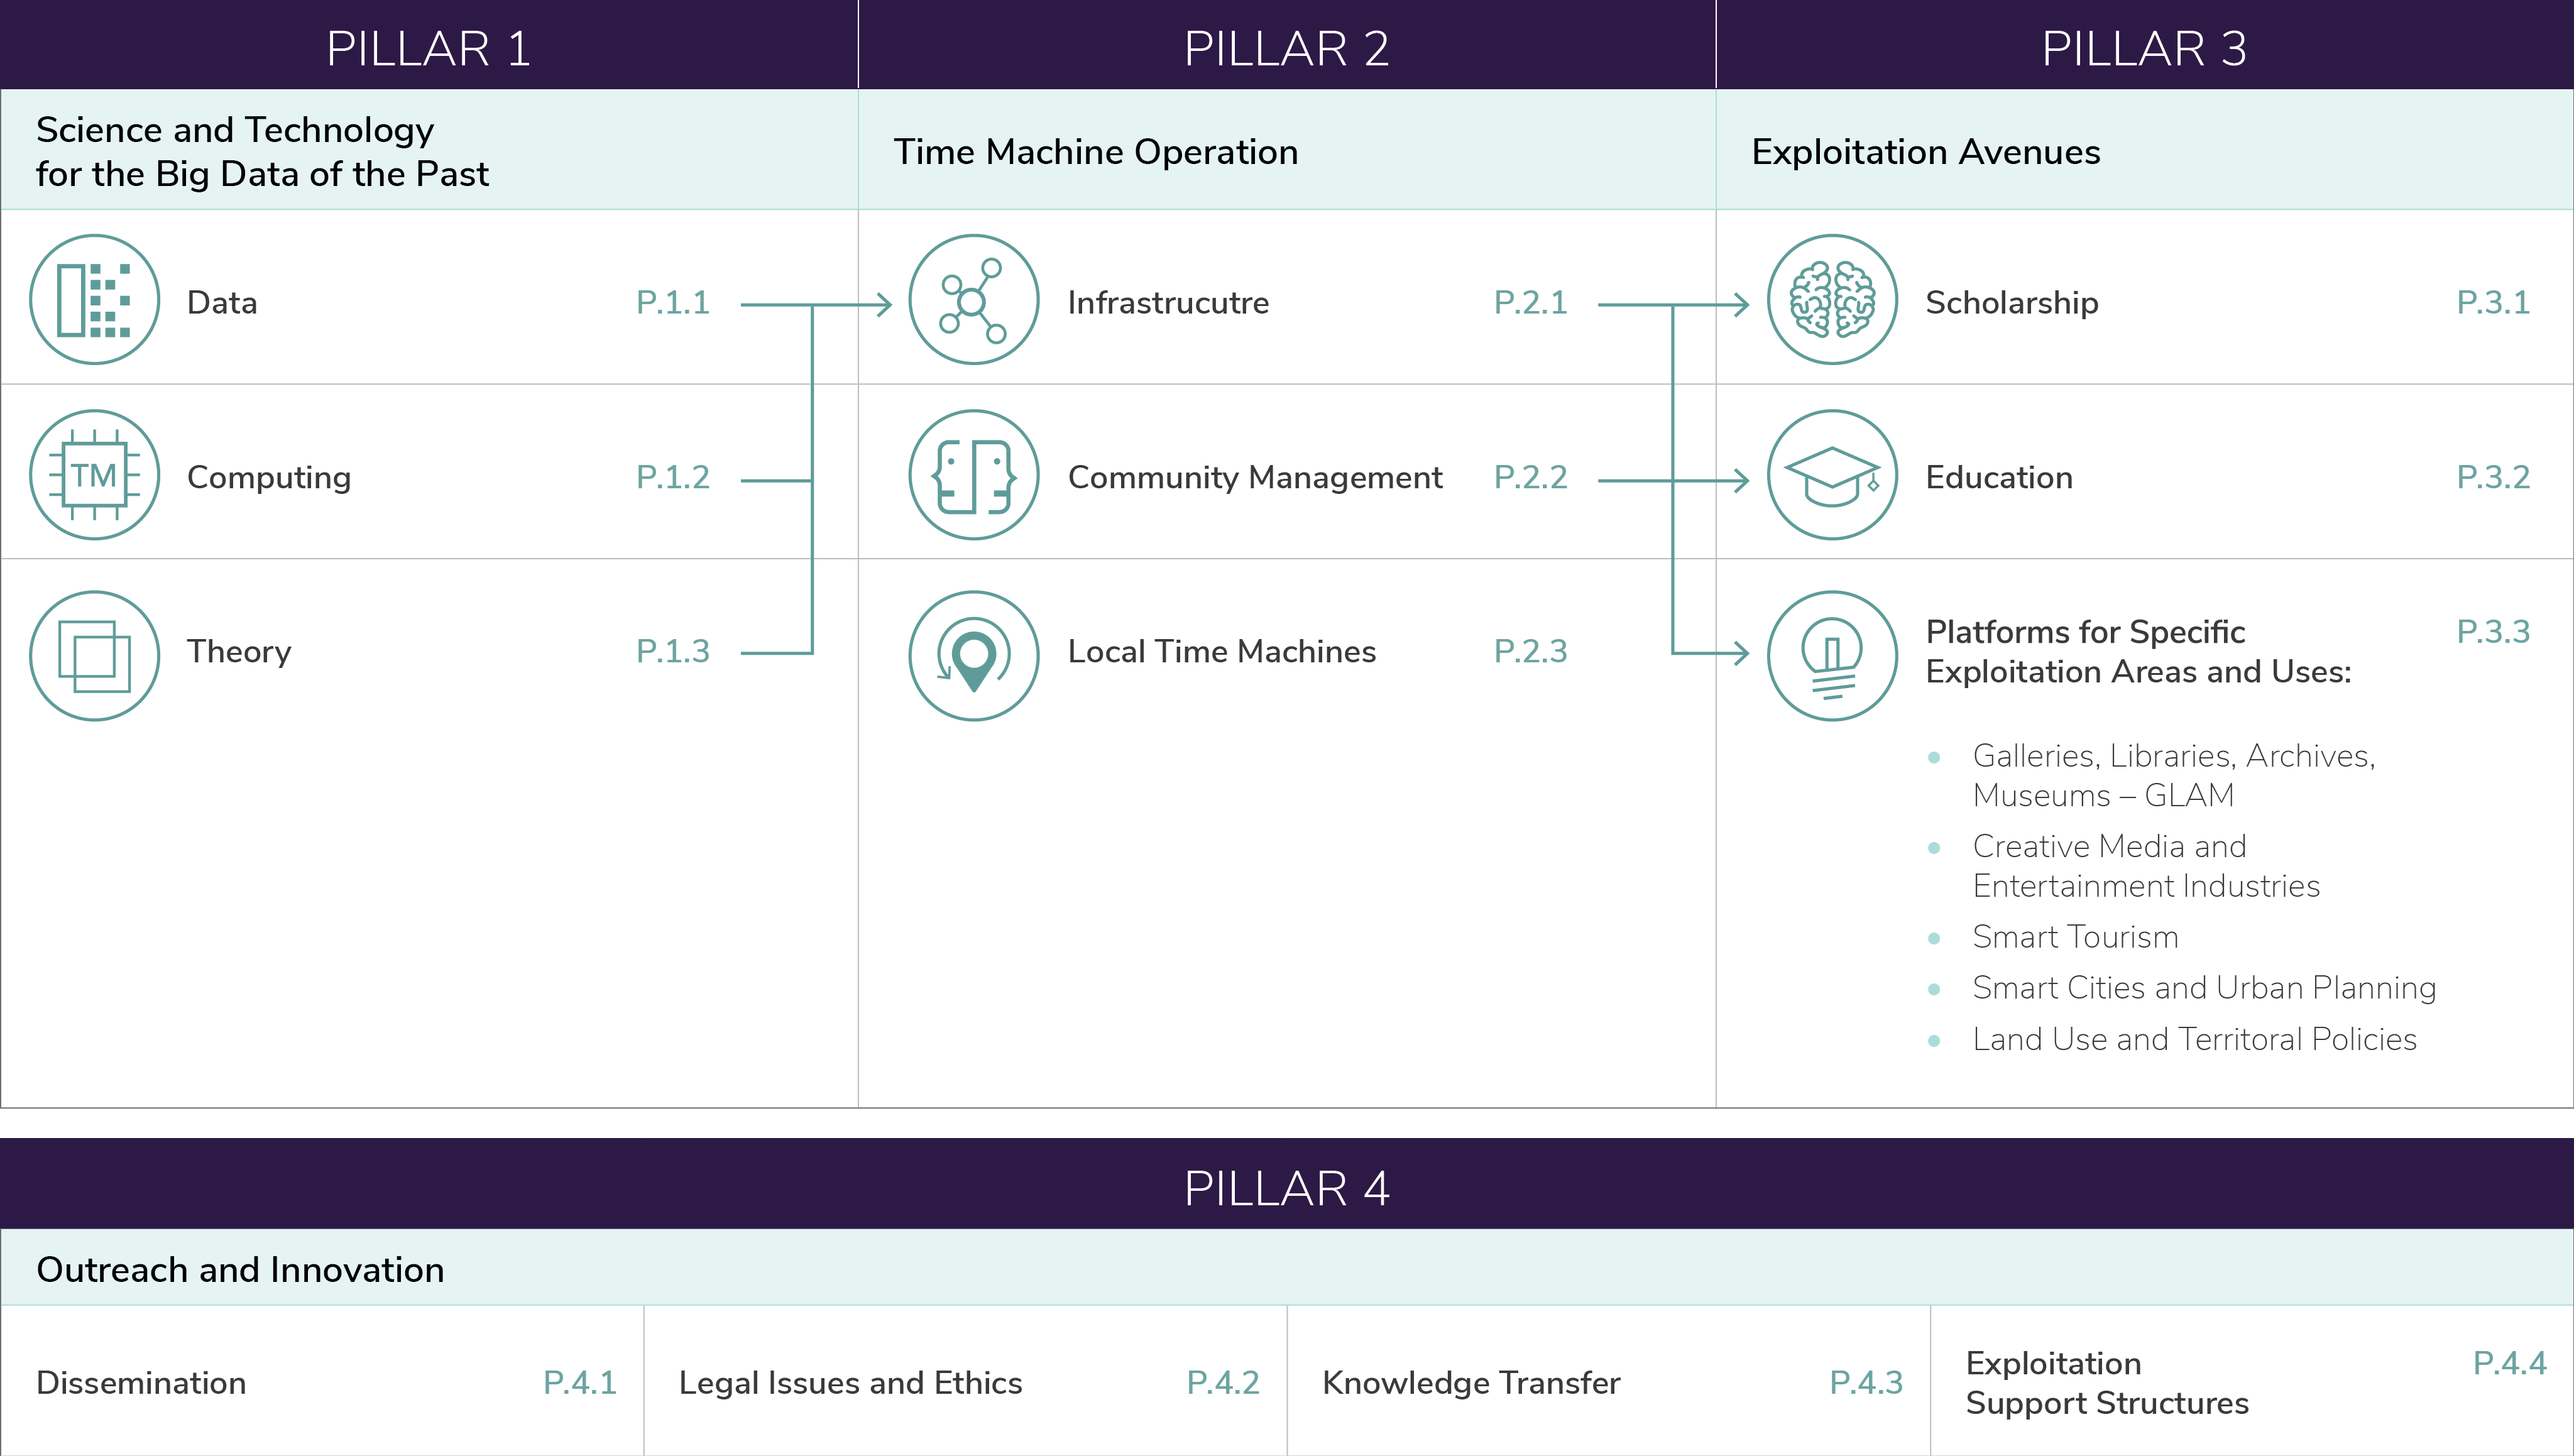
\includegraphics[width=15cm]{pillar_org.png}
\caption{Organisation et interactions des premiers \textit{PILLAR}s \textit{© Copyright 2019 Time Machine}}
\end{figure}

Cette période du \gls{csa} est également rythmée par différentes conférences\footnote{Nous participerons à la deuxième conférence, réunissant les groupes de travail des différents \textit{PILLAR}, les 9-10 mai à Amsterdam}, visant à réunir les partenaires afin de faciliter la collaboration au sein des membres d'un même PILLAR ou \gls{wp}, de faire connaître le projet et d'inviter les membres croissants à collaborer à ce processus décisionnel. En effet, le réseau Time Machine grandit en parallèle de la période du \gls{csa} et bien que les nouveaux membres ne soient pas liés contractuellement à l'élaboration du projet, ni rémunérés par l'\gls{ue}, les échanges sont fortement encouragés. Lors de la conférence d'Amsterdam des 9 et 10 mai 2019, plus d'une centaine de participants ont fait le déplacement.

Bien que très vite, la perspective du milliard d'euros ait été retirée\footnote{Détails dans le chapitre \ref{fet}.}, les participants ont poursuivis le plan d'élaboration et des rendus fixés par l'\gls{ue}, dans l'attente que les commissions concernées trouvent la manière appropriée de \inquote{faire atterrir} le projet, étant toujours liés contractuellement puisqu'ayant touché le million. 

La période de notre stage coïncide avec la recherche de nouvelles formes de financement et de pressions auprès de l'\gls{ue} conduites par le comité exécutif, en vue de demeurer un projet bénéficiant du soutien européen.

\section{Déroulement du stage}

Les missions du stage, initialement attachées à l'étude et à l'implémentation d'un des composants du réseau Time Machine précédemment mentionné, la \textit{Time Machine Box}\footnote{\cite{epfl.dhlab_home_nodate}} ont été modifiées dès notre premier jour. Notre maître de stage, ayant évalué qu'il serait plus intéressant de nous impliquer dans la conception du réseau de \textit{Local Time Machines}, ce qui correspond au \textit{PILLAR 2}. 

Concrètement, nous avons eu pour mission de rendre début juin 2019 la première version de la feuille de route du projet à destination de l'\gls{ue}, en charge de valider les différentes propositions. Une période de consultation des propositions contenues étant planifiée de juillet à septembre, avant le rendu final devant avoir lieu à la fin de l'année 2019. 

Notre stage a consisté en la création de la première proposition de ladite feuille de route pour le \textit{PILLAR 2}, en étroite collaboration avec notre maître de stage, des membres d'Icarus\footnote{\cite{icarus_icarus_nodate}} et le consultant du projet\footnote{Vous trouverez ladite feuille de route sur la clé USB jointe au mémoire.}. La version finalisée de la feuille de route devant être développée pour décembre, elle ne fait pas partie de nos missions de stage. 

Le \textit{PILLAR 2} se compose de trois grandes sections, la première traitant de l'infrastructure (sous la responsabilité du Professeur Frédéric Kaplan), la deuxième des communautés (sous la responsabilité des membres d'Icarus) et la troisième des enjeux organisationnels et opérationnels du réseau de Time Machines locales et par conséquent du projet Time Machine dans son ensemble. Nous fûmes responsable de la troisième section et de l'articulation des différentes parties les unes avec les autres, avec pour objectif de garantir la cohérence entre les propositions de recherche identifiées dans le \textit{PILLAR 1}, et les impacts envisagés par le \textit{PILLAR 3}. Mettre en place les opérations et l'infrastructure nécessaires à un réseau tel que Time Machine sous-tend de définir chacun de ses composants et leurs rôles respectifs et de précisément établir le cadre, ce que nous nous sommes efforcée de faire afin de pouvoir définir les directives associées. 

La création de cette première version s'est déroulée suivant quatre étapes qui ont rythmé nos activités de stagiaire : 

\begin{enumerate}
\item \textbf{Définition}

Clarification du contexte, des différentes instances et partenaires du réseau Time Machine et de leurs rôles respectifs.
\item \textbf{Écriture}

Transformation des idées définies en 1 en objectifs et réalisations concrètes. Rédaction de la feuille de route.
\item \textbf{Intégration et validation}

Consultation et évaluation des propositions par les partenaires et intégration des commentaires. Création de la cohérence entre les différentes feuilles de route proposées en \textit{PILLAR 1} et \textit{PILLAR 3}. 
\item \textbf{Consultation externe}

Définition de questions ciblées pour la phase de consultation externe, ouverte au grand public.
\end{enumerate}

Nous avons été aidée dans la réalisation de notre mission par les membres du \gls{dhlab} et particulièrement par la coordinatrice de la \textit{Venice Time Machine}, Dr. Isabella di Lenardo, membre également de l'unité de coordination du projet Time Machine\footnote{Nous participerons à un voyage d'étude à Venise (30 mai au 1\up{er} juin 2019), pour découvrir les coulisses de la \textit{Venice Time Machine}.}.
\newpage

\begin{figure}[H]% force à placer l'image au sein de notre balise figure
%\centering
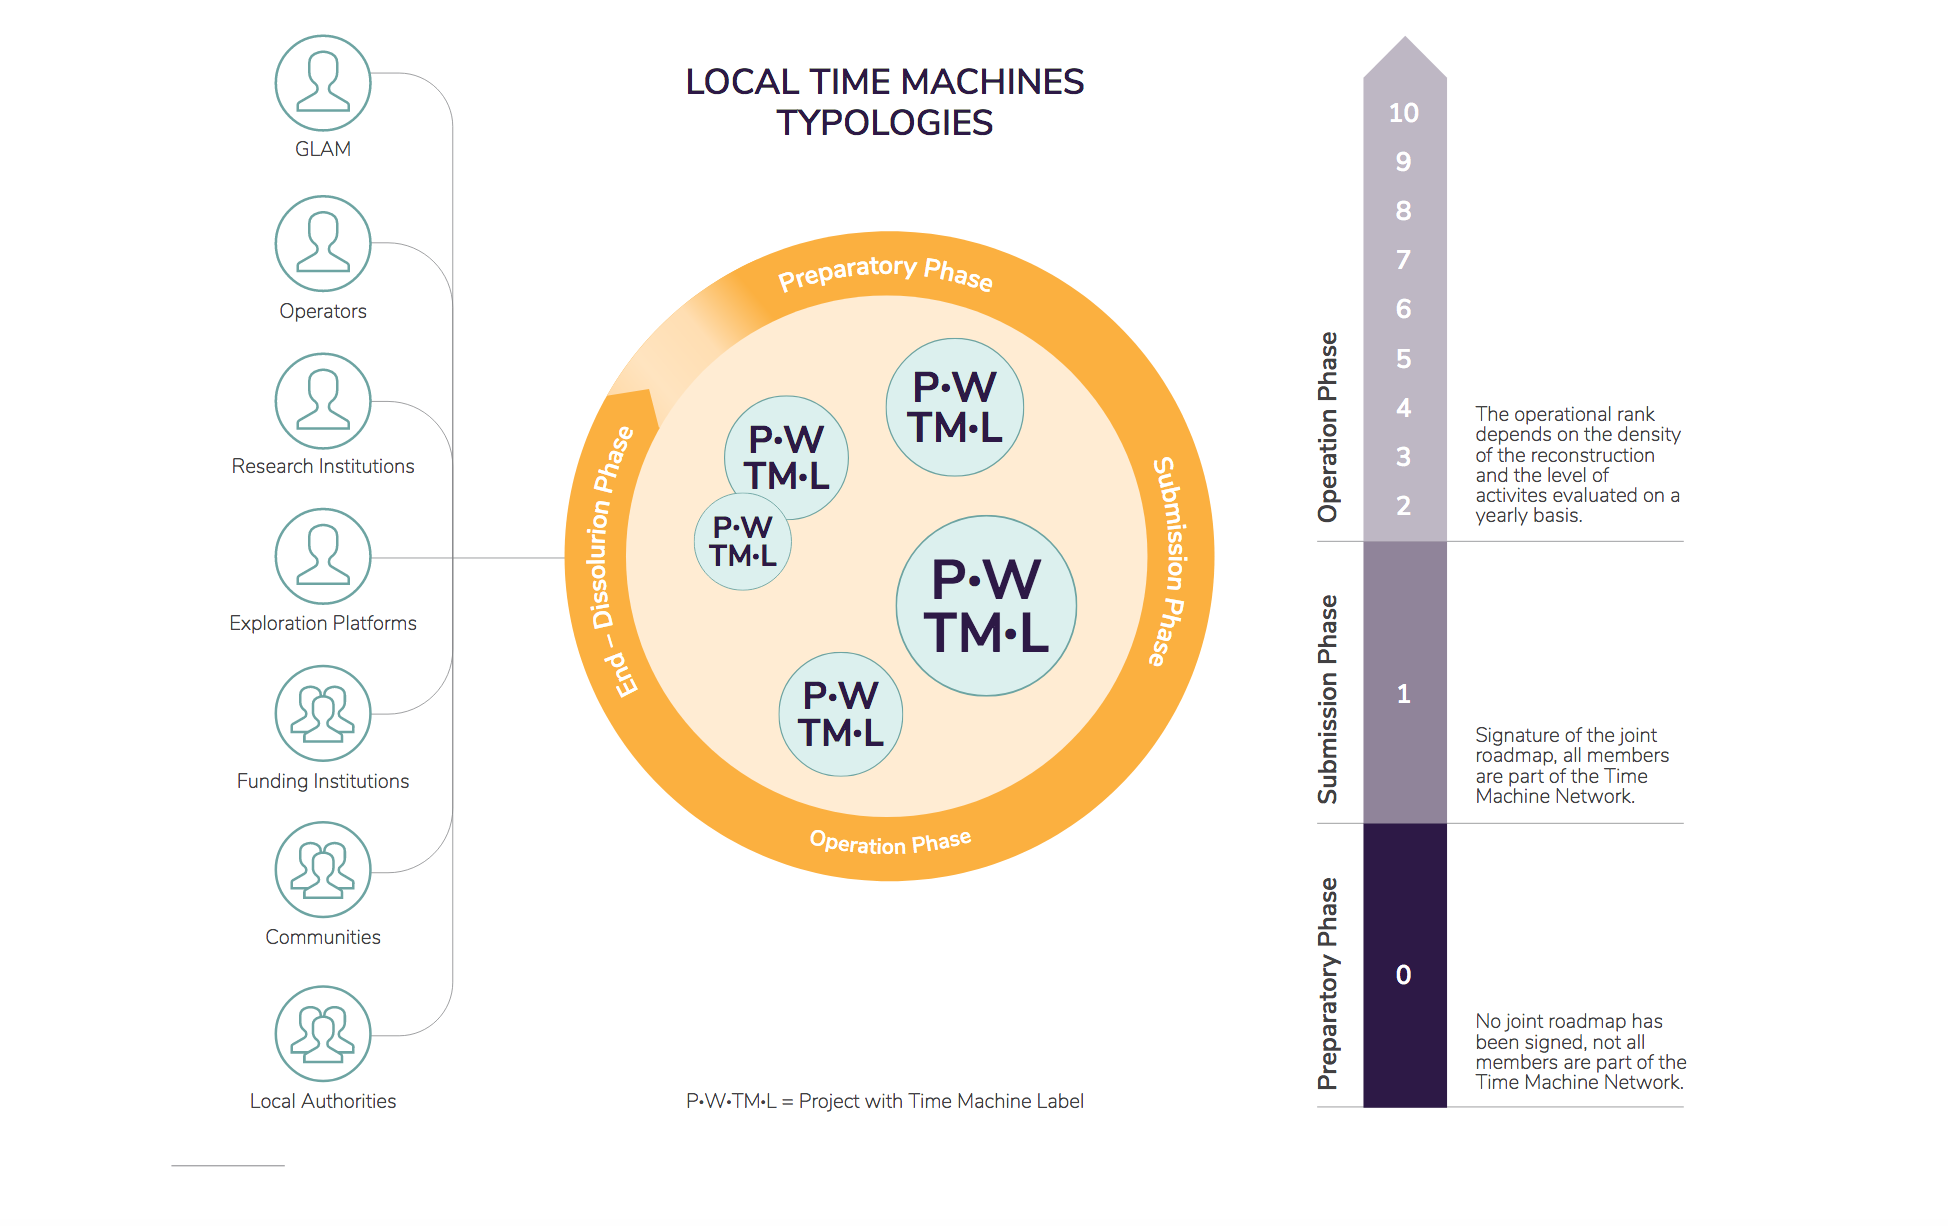
\includegraphics[angle=90, scale=0.7]{ltm.jpg}
\caption{Local Time Machines, document de travail \textit{© Copyright 2019 Time Machine}}
\end{figure}


\section{Rédaction de la feuille de route}

L'élaboration de la feuille de route s'est très vite révélée une tâche ambitieuse, puisqu'elle implique à la fois l'intégration des idées motrices à l'initiative Time Machine, telles que pensées par le \gls{dhlab}, dans le contexte de la recherche en humanités numériques, et la prise en compte des envies et attentes des différents partenaires. Rédigée à destination d'un réviseur mandaté par l'\gls{ue} et dans le but d'obtenir un financement, ce document doit à la fois faire rêver et concrétiser les idées de tous. 

Nous nous sommes vite trouvée confrontée à la réalité que derrière le nom du projet et la quête commune visant à proposer un \gls{graph} du passé, se cachaient autant de définitions que de membres du réseau. Notre travail de stagiaire a consisté en un difficile exercice de transcription de tous ces intérêts parfois divergents, parfois audacieux, vers une feuille de route commune, servant de base au futur cadre des opérations, mais suffisamment flexible et vaste pour intégrer les inévitables changements induits par sa longue durée et son financement des plus incertains. Mener à bien cette mission nous a poussée à comprendre très précisément les différents composants du futur réseau Time Machine, qu'ils soient d'ordre technique ou opérationnel. Le projet étant prévu pour se déployer sur dix ans, la feuille de route reste à un niveau relativement macro, puisqu'il est difficile de prévoir certains choix techniques ou stratégiques avant que l'infrastructure, le financement et la gouvernance ne soit eux-mêmes clarifiés.

Au début de notre stage, le projet en est à ses prémisses, tout reste à définir et les nombreuses questions que nous nous posons ne font que s'ajouter à la longue liste de celles auxquelles nous devons proposer une réponse, et celles qui sont posées par les membres du comité exécutif. Le temps n'est d'ailleurs pas aux palabres et à la réflexion, puisque l'échéance du rendu intervient tôt, nous n'avons malheureusement pas eu l'opportunité de mener l'intégralité du travail réflexif présenté dans ce mémoire avant le rendu de la feuille de route. Ce travail de recherche nous a d'ailleurs permis de remarquer certains manques qui seront signalés.

Notre méthodologie de travail s'est construite autour des éléments et des enjeux figurant dans la première proposition du projet faite à l'\gls{ue}, complétée par nos discussions avec les membres du consortium, du comité exécutif, les équipes du \gls{dhlab} et notre maître de stage. 

Travaillant au sein d'un environnement ouvert où chaque membre peut suivre la construction des idées de manière transparente, nous avons également bénéficié de remarques ciblées émanant de certains spécialistes partenaires du consortium.
%===ajouter une mention de où accéder à la roadmpa
Les premières semaines de notre stage ont consisté en un grand travail de définition, afin de proposer un socle commun construit autour d'une clarification du contexte des différents éléments du projet, sur lequel chaque \gls{wp} ou \textit{PILLAR} peut venir appuyer ses idées. Ce travail a conduit à l'élaboration de différents graphiques et documents, qui trouvent une version plus synthétisée dans la deuxième partie de la feuille de route, \textit{Pillar 2 Key concepts}. 

Nous avons également été confrontée à la difficulté que chacun des trois premiers \textit{PILLAR}s, bien que planifiés pour être écrits en parallèle, était destiné à influencer les choix des autres. Veiller à articuler ces propositions pour garantir une harmonisation des processus (entre les pistes de recherche identifiées dans le \textit{PILLAR 1} et les impacts envisagés par le \textit{PILLAR 3}) a impliqué des ajustements jusqu'aux derniers jours avant le rendu. Le détail de ces interactions figure également dans la deuxième partie de la feuille de route, \textit{Interaction of pillar 2 with pillars 1 and 3}. 

De manière générale, la construction de la feuille de route a nécessité une grande flexibilité, et de nombreuses versions ont vu le jour avant d'aboutir à celle introduite dans ce mémoire et disponible en annexe\footnote{La version soumise à l'\gls{ue} fait quelque 60 pages et est écrite en anglais. Vous pouvez la consulter sur la clé USB accompagnant ce mémoire.} Écrit à plusieurs mains, ce document, à la hauteur des projets de numérisation, est complexe, et chaque choix pourrait être analysé. 

Pour ne pas alourdir inutilement ce rendu et rester dans le cadre de notre problématique, nous ciblons notre présentation sur les réponses apportées par Time Machine aux enjeux de la numérisation. Bien que ces derniers ne soient pas décrits ainsi dans la feuille de route, les différentes solutions développées dans la partie trois \textit{Research and Innovation Plan}, complétés des éléments proposés par les autres \textit{PILLARs} et \gls{wp}s contribuent à y répondre et offrent un aperçu cohérent de notre expérience de stagiaire. 

La feuille de route figure sur la clé USB accompagnant ce mémoire.

\begin{figure}[ht]% force à placer l'image au sein de notre balise figure
%\centering
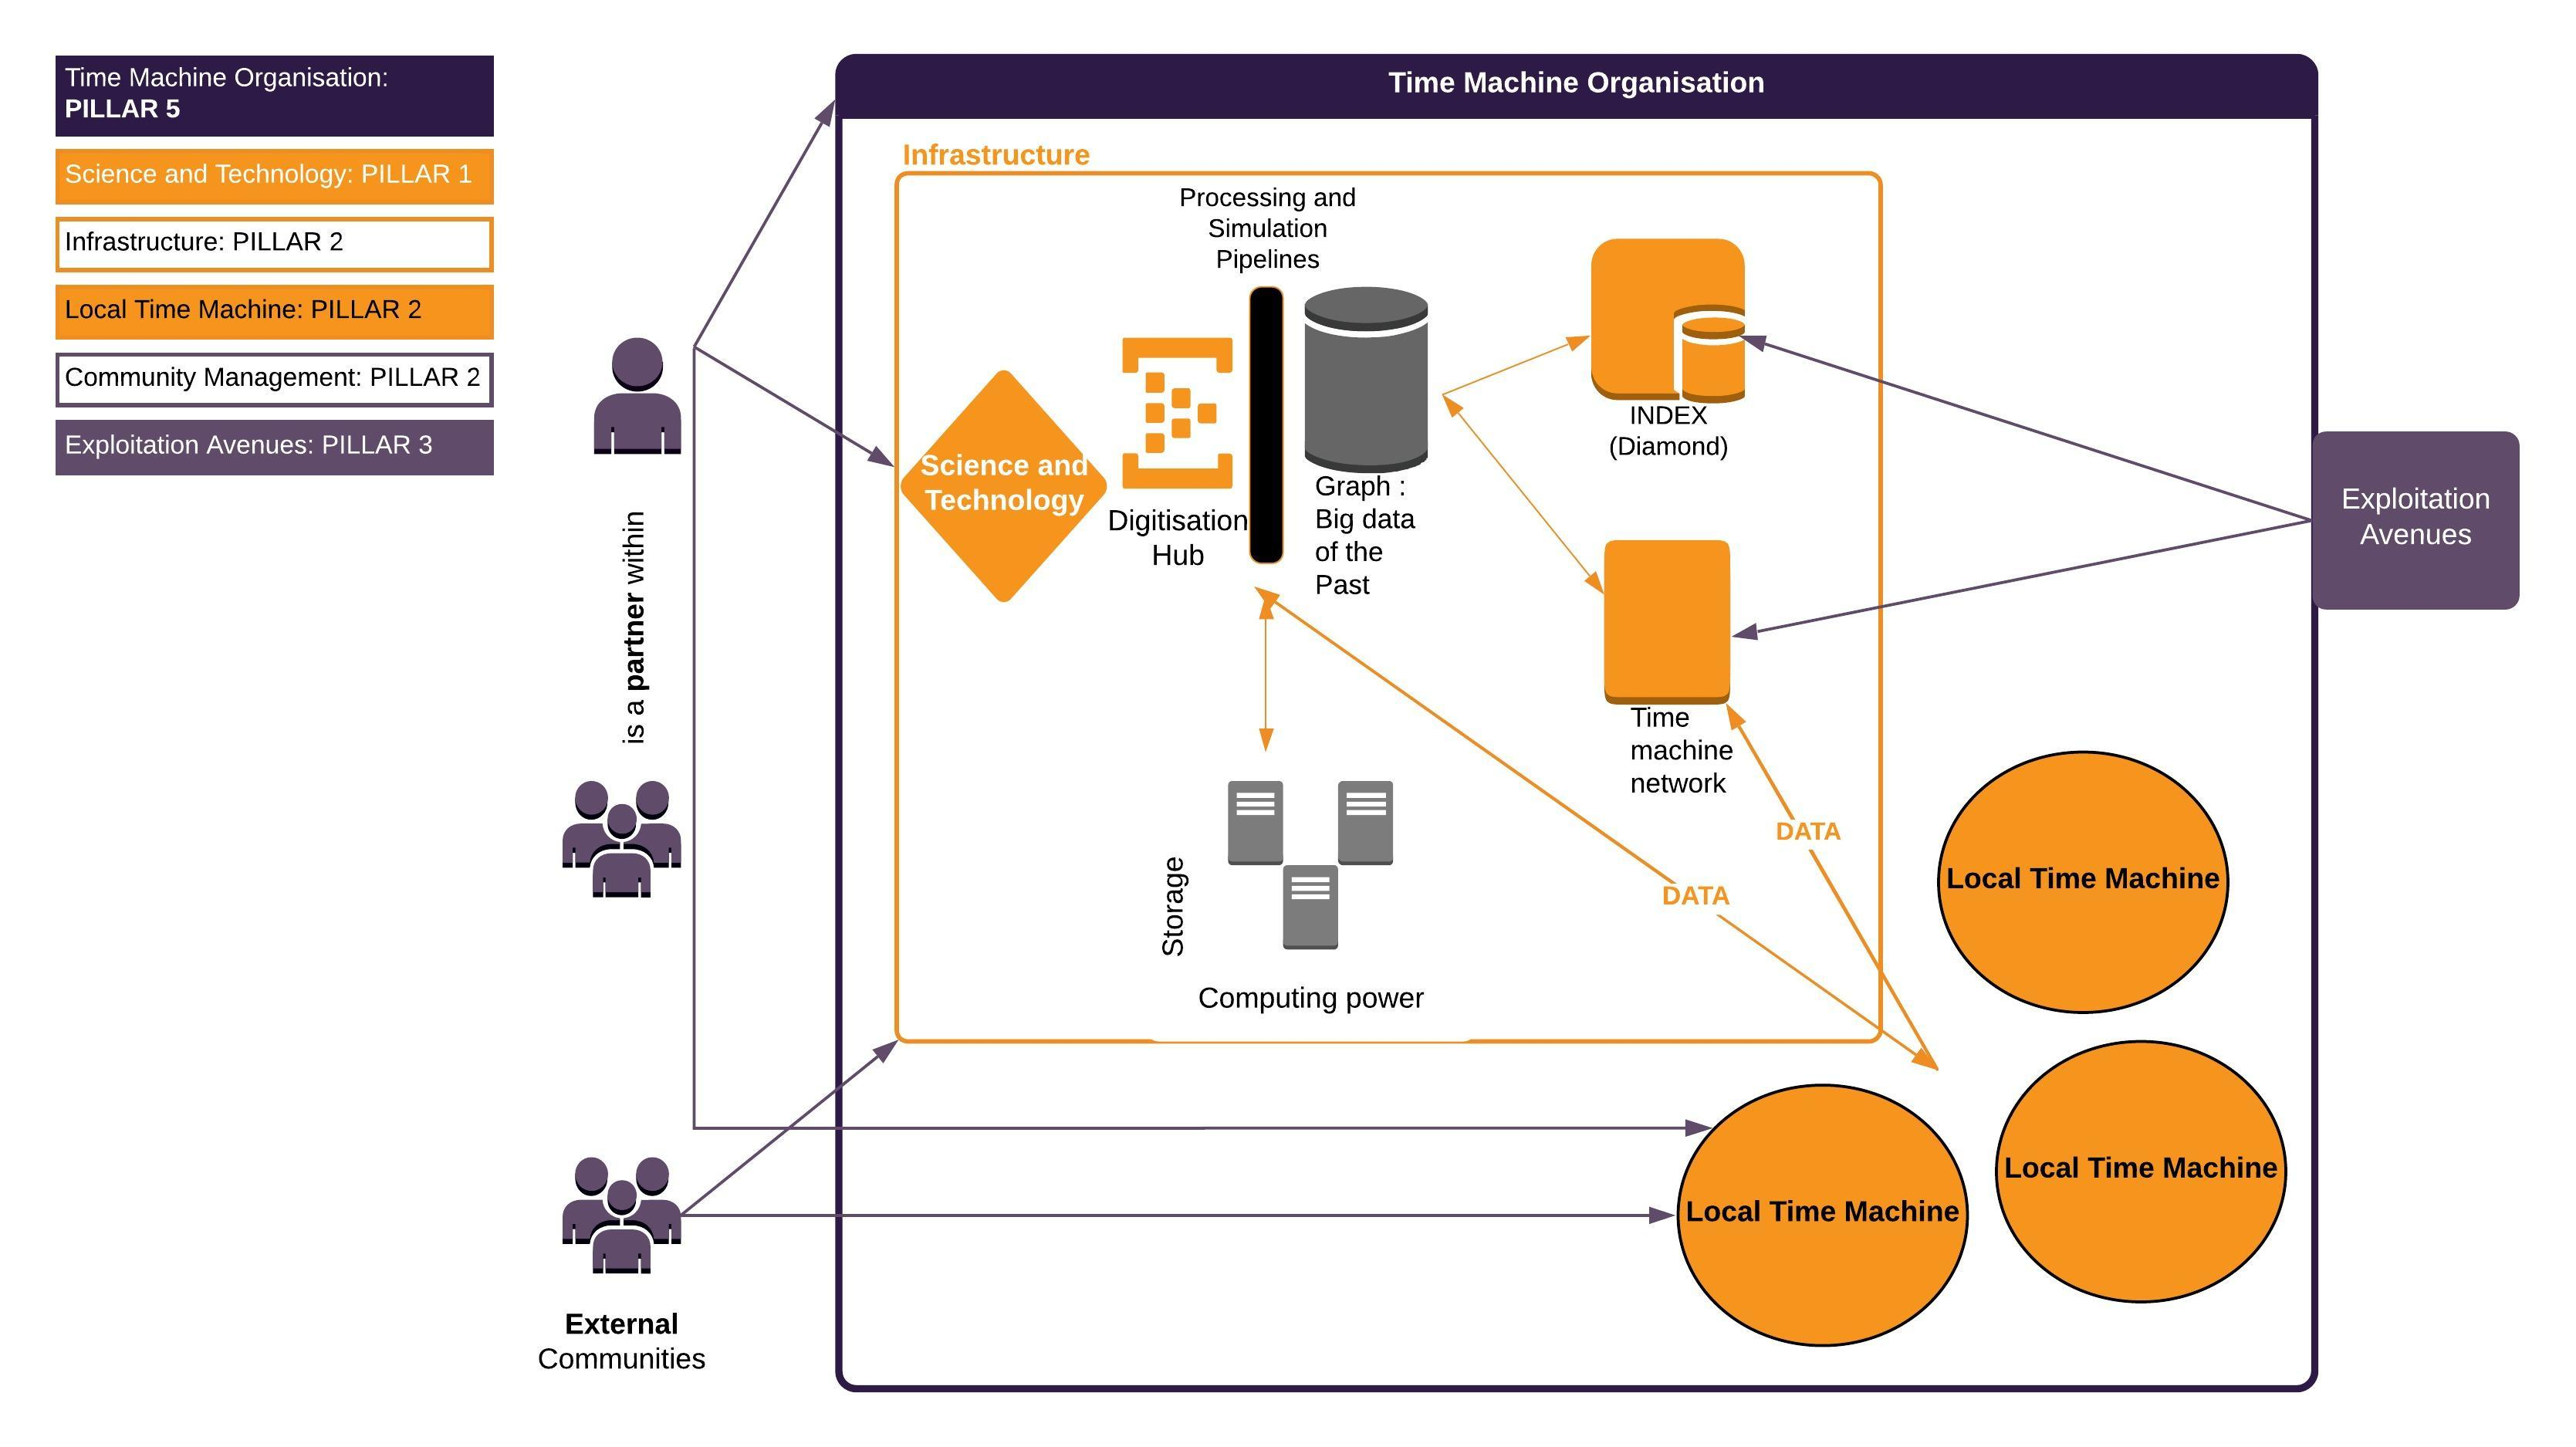
\includegraphics[angle=90, scale=0.9]{tmo.jpeg}
\caption{Les différents composants de la \textit{Time Machine Organisation}, document de travail}
\end{figure}

%==== REPONSES APPORTEES PAR TM AUX ENJEUX DE LA NUMERISATION
\chapter{Quelles réponses aux enjeux de la numérisation ?}

Le projet Time Machine étant encore dans un processus de définition, nous ne pouvons garantir que les propositions énoncées ci-après seront réellement implémentées après la période du \gls{csa}. Toutefois, elles reflètent les premières hypothèses et volontés organisationnelles, qui seront amenées à se concrétiser plus précisément au fil de l'avancement du projet.

\section {Amener différents acteurs à collaborer}
Time Machine est par essence un projet collaboratif qui vise à agréger les données de différentes institutions culturelles et patrimoniales.

Né d'une association de 33 institutions, le consortium compte désormais plus de 300 membres. Pour parvenir à co-construire ce projet, la collaboration est centrale à différents niveaux : entre les  partenaires appelés à concevoir l'organisation du projet et à partager des ressources ; entre le projet et les instances extérieures qu'elles soient politiques, académiques, privées, publiques ; entre le projet et le grand public. Afin de préserver ces relations, différentes démarches ont été entreprises et le déploiement des solutions contenues dans la feuille de route devront contribuer à préserver le futur de cette coopération. 

Conscients de l'importante de la collaboration pour une initiative de cette envergure et par conviction du pouvoir de l'intelligence collective, la collaboration sera intégrée aux futures valeurs du projet. Différents moyens seront mis en place afin de promouvoir l'existence d'espaces d'échanges et encourager un décloisonnement des activités au profit d'une logique de groupe. Un système de label sera par exemple développé afin d'encourager les différents projets composant Time Machine à favoriser cette pratique (des moyens qualitatifs serviront à l'évaluer).

Afin de favoriser l'acceptation, le développement et la mise à jour des futurs standards du réseau, un processus inspiré de celui utilisé pour définir les standards d'internet sera adopté : \gls{rfc}\footnote{Pour en savoir plus : \url{https://en.wikipedia.org/wiki/Request_for_Comments}}. Ce système consiste en la publication en ligne de propositions, dont les thématiques, voir les pistes de réponses, ont d'abord été définies par un comité d'édition en fonction des besoins du projet. Publiées de manière transparentes, elles sont soumises à la validation et aux critiques de la communauté, et ne sont implémentées que lorsque le consensus est atteint. La feuille de route contient de nombreuses propositions de \gls{rfc}s visant à mettre en place l'infrastructure et les opérations.

Le projet s'inscrivant dans une démarche de transparence, les composants techniques, ainsi que toute la documentation du projet seront accessibles sous licences \textit{\gls{cc}}, favorisant leurs réutilisations et le développement de nouveaux services. Le partage des connaissances et les développements technologiques font partie des objectifs du projet, qui s'inscrit dans la démarche d'\gls{os}.

Partenaire de grand réseaux culturels et patrimoniaux (à l'instar d'Europeana), Time Machine s'attachera à mettre en place des moyens dédiés à favoriser synergies et interactions entre ces différents acteurs, favorisant les échanges de bonnes pratiques et contribuant à l'accroissement des activités de ces réseaux et le développement d'outils communs. 

Les communautés de bénévoles spécialistes ou amatrices seront invitées à prendre une part active au sein des projets. Inscrivant Time Machine dans la mouvance des \gls{cs}.

Au sein de chaque Time Machine locale, un espace \textit{Smart Clusters}, servira à rassembler les potentiels futurs exploitants (industries culturelles et créatives, industries touristiques, instances politiques régionales etc.) et les partenaires de Time Machine, afin  d'impliquer les premiers dans la conception de projets, et assurer un ancrage de l'initiative locale au sein de son environnement et le déploiement d'une partie de ses activités autour de particularités et besoins ciblés.

\subsection{\textit{Complément} aux propositions de la feuille de route :}

Les données produites au sein des Time Machines locales étant destinées à alimenter le \gls{graph} du passé, ces dernières constituent un réseau de partenaires (\gls{agr}s) stratégiques, avec lesquels il faut particulièrement soigner la collaboration. La mise en place d'un forum similaire à celui d'Europeana ou \gls{dpla} favorisant les échanges devrait ainsi être considéré. La place des \gls{agr}s thématiques et régionaux déjà existants devra également être réfléchie.

\section {Financement et partenariats public-privé}

Un modèle de franchise sera mis en place, permettant aux différents partenaires de bénéficier de l'infrastructure de Time Machine, de formation et d'aide ciblée tout en contribuant à l'autonomie financière du projet. Ce dernier tiendra compte de différents critères et visera à clarifier les relations entre les Time Machines locales et la future gouvernance. 

Au-delà des partenariats financiers, le réseau mise sur la création de la \textit{Time Machine Infrastructure Alliance}, regroupant des partenaires extérieurs au projet mais intéressés à contribuer au développement de nouvelles technologies, et des philanthropes, qui seront invités à participer par des moyens plus concrets (puissance de calcul informatique, espace de stockage) à la durabilité du projet. 

Les différentes Time Machines locales seront à priori responsables du financement de leurs projets. 

Le consortium étant déjà composé d'un mélange entre partenaires publics et privés, cette spécificité sera conservée au sein de la future \textit{Time Machine Infrastructure Alliance}. Une attention particulière sera portée sur ces partenariats afin de garantir la mission de transparence et d'ouverture que s'est donné le projet. 

Il est possible que des institutions privées souhaitant bénéficier des outils de Time Machine puissent le faire, sans que leurs données soient utilisées pour alimenter le futur \gls{graph} de données du passé, ces dernières devront payer pour ce service en fonction d'une tarification préétablie.

Le financement servant à développer l'infrastructure du projet, n'est pas encore connu, mais le projet est en quête du soutien de l'\gls{ue}.


\section {Droit d'auteur}

Time Machine est amené à traiter deux typologies différentes de données : les privées et les publiques. Les données publiques (produites par des institutions publiques, ou données libres de droit) seront partagées sous licences \textit{\gls{cc}}, de préférence CC0. Les données privées (produites par des particuliers ou des institutions privées, données personnelles, ou données sous droit) seront protégées par des licences plus strictes et leur consultation pourra être sujette à certaines restrictions. Les données à caractère sensible (violentes ou illicites) publiées sous licence \textit{\gls{cc}}, seront également associées à des restrictions d'accès. 

Les différentes licences seront explicitées dans les métadonnées de chaque document. 

Les outils et processus permettant de faire face à ces typologies de données restent encore à déterminer.

\subsection{\textit{Complément} aux propositions de la feuille de route :}

La feuille de route ne mentionne pas précisément le besoin de créer et rendre visible un système de déclarations des droits d'usage pour améliorer l'accès aux ressources. Le traitement des \oe{}uvres orphelines ou hors commerce n'est pas non plus abordé alors que, suite aux exemples étudiés, nous préconiserions l'étude d'une stratégie de gestion des risques pour ces \oe{}uvres au statut légal incertain.

\section {Sortir des silos : enjeux techniques}

Europeana étant partenaire du réseau Time Machine, à priori son modèle de métadonnées (suivant les recommandations du modèle RDF) sera utilisé au sein du projet (pour les données non déduites) et l'architecture de Time Machine sera interopérable avec celle d'Europeana. Un modèle pour les données déduites sera élaboré, s'assurant de faire figurer explicitement les processus de création de ces informations dans leurs métadonnées. Une charte technique, contenant ces différentes spécifications devra être signée par tous les partenaires du réseau Time Machine. Time Machine prendra part aux réflexion menées sur les vocabulaires contrôlés \footnote{Rappel : Lexique servant à organiser les connaissances pour favoriser la recherche d'information} et les ontologies\footnote{\inquote{Rappel : Une ontologie est une façon de modéliser un domaine en identifiant les concepts y afférents et en les organisant les uns par rapport aux autres \cite{delestre_du_2017}.} }

En plus de la standardisation des métadonnées, Time Machine vise à normaliser les protocoles de numérisation, afin de garantir une qualité et une cohérence à travers tous les centres de son futur réseau européen de numérisation. 

Time Machine rendra obligatoire l'utilisation de \gls{iiif} pour les images, veillera au déploiement de différentes \gls{api}s et utilisera le protocole \gls{oai} .

\subsection{\textit{Complément} aux propositions de la feuille de route :}
La qualité de la numérisation devra être suffisamment élevée pour garantir un stockage sur le long-terme des données numérisées et les critères de cette qualité précisément étudiés.

En plus de l'usage de \gls{iiif}, \gls{oai} et autres \gls{api}s pour garantir l'interopérabilité, il serait judicieux d'offrir la possibilité aux futurs exploitants de disposer d'une exportation totale des bases de données (suivant l'exemple de \gls{dpla}).


\section {Sortir des silos : enjeux sur le contenu}

Mise en place d'un système de sélection des données (politique documentaire) s'inspirant des recommandations élaborées par \textit{The National Information Standards Organisation}\footnote{Pour en savoir plus : \url{https://www.niso.org/}.}, qui sont basées sur des critères liés aux besoins de recherche des institutions, unicité des documents, valeur du document etc. Bien qu'ayant vocation à numériser toutes les données du passé, il est probable que certains documents servant de base au développement de la future plateforme soient numérisés en premier (tels que les cadastres, journaux, cartes et plans). Time Machine ne se focalise pas sur un seul format de document et veut développer particulièrement la numérisation 3D.

\subsection{\textit{Complément} aux propositions de la feuille de route :}
Les manques hérités des politiques de numérisation des institutions partenaires, ou les différents biais qui peuvent être amenés à persister dans de nouvelles initiatives, devraient être étudiés et certains projets spécifiquement entrepris afin de rétablir l'équilibre.

Certaines mesures spécifiquement dédiées à faciliter la numérisation de données à partir du 20\up{e} siècle devraient être examinées afin de contribuer à sortir l'Europe de ce \inquote{trou noir} de l'information.


\section {Stockage sur le long-terme - préservation}

La préservation sur le long-terme des données de Time Machine sera prise en compte par le projet, afin que l'énorme travail de numérisation n'encourt pas le risque d'être perdu.

Time Machine propose des solutions de stockage à destination des petites institutions qui ne disposent pas d'espace suffisant sur leurs propres serveurs : les \textit{Time Machine Box}. Ces dernières existent à l'état de prototype et devront être améliorées (elles ne disposent pas encore de copie de sauvegarde).

Les données du projet seront stockées de manière partagée (à travers les ressources de la \textit{Time Machine Infrastructure Alliance}) sur des serveurs  spécialement conçus pour garantir leur préservation durable et prévenir tous risques d'accidents ou de dommages. 

Le poids des jeux de données et l'impact environnemental des serveurs faisant partie des préoccupations du projet, des solutions de stockage innovantes sont aussi envisagées.

\newpage
\section{Résumé des réponses de Time Machine aux enjeux de la numérisation}
\begin{table}[H]
\centering
\begin{tabular}{|l|l|}
\hline
\rowcolor[HTML]{2E1A46} 
{\color[HTML]{FFFFFF} \textbf{Enjeux}}                                                                                   & {\color[HTML]{FFFFFF} \textbf{Réponses de Time Machine}}                                                                                                                                                                                                                                                                                                                                                                                                                                           \\ \hline
{\color[HTML]{2E1A46} \textbf{\begin{tabular}[c]{@{}l@{}}Amener différents\\ acteurs à collaborer\end{tabular}}}         & \begin{tabular}[c]{@{}l@{}}Inscription de la collaboration dans les valeurs du projet et \\ création d'un système de labels. Utilisation des \textit{Request for}\\ \textit{Comments}. Publication et partage des différents développements \\ sous licence \textit{Creative Commons}. Échange avec les réseaux \\ partenaires. Intégration du grand public (sciences citoyennes).\\ Création de \textit{Smart Clusters}. Création d'un forum favorisant les\\ échanges entre les Time Machines locales et la gouvernance.\end{tabular} \\ \hline
{\color[HTML]{2E1A46} \textbf{\begin{tabular}[c]{@{}l@{}}Financement et \\ partenariats \\ public-privé\end{tabular}}} & \begin{tabular}[c]{@{}l@{}}Moyens financier assurés par les partenaires (redevance). \\ Soutien en nature possible à travers la \textit{Time Machine}\\ \textit{Infrastructure Alliance}. Vente de services à l'extérieur du \\ projet. Les Time Machines locales sont responsables du \\ financement de leurs projets. Partenariats public-privé déjà \\ existants et amenés à se développer. Recherche de financement \\ pour l'infrastructure auprès des instances européennes.\end{tabular}                   \\ \hline
{\color[HTML]{2E1A46} \textbf{Droit d'auteur}}                                                                           & \begin{tabular}[c]{@{}l@{}}Favorable à l'usage des licences \textit{Creative Commons}. \\ Restriction d'accès dans le cadre de données privées \\ ou sensibles. Métadonnées explicites. Déploiement \\ d'un système de déclaration des droits d'usage.\end{tabular}                                                                                                                                                                                                                                         \\ \hline
{\color[HTML]{2E1A46} \textbf{\begin{tabular}[c]{@{}l@{}}Sortir des silos : \\ enjeux techniques\end{tabular}}}          & \begin{tabular}[c]{@{}l@{}}Adoption du modèle de métadonnées développé par Europeana \\ et interopérabilité avec sa plateforme. Recours à des \\ vocabulaires contrôlés. Utilisation des différents outils tels que\\ APIs, IIIFs, OAI-PMH. Création de normes de qualité pour la \\ numérisation, amenées à se déployer à travers les futurs centres \\ de numérisation du réseau Time Machine.\end{tabular}                                                                                       \\ \hline
{\color[HTML]{2E1A46} \textbf{\begin{tabular}[c]{@{}l@{}}Sortir des silos : \\ enjeux sur le \\ contenu\end{tabular}}}   & \begin{tabular}[c]{@{}l@{}}Politique documentaire. Intégration des différentes typologies \\ de données et développement spécifique de la 3D. Analyse des\\ manques existants et actions ciblées pour y pallier.\end{tabular}                                                                                                                                                                                                                                                                        \\ \hline
{\color[HTML]{2E1A46} \textbf{\begin{tabular}[c]{@{}l@{}}Stockage sur le \\ long-terme - \\ préservation\end{tabular}}}  & \begin{tabular}[c]{@{}l@{}}Développement de solutions de stockage pour les petites\\ institutions. Le stockage des données sur le long-terme est\\ essentiel. Les données seront stockées pour être préservées \\sur les serveurs de la \textit{Time Machine Infrastructure Alliance}.\end{tabular}                                                                                              \\ \hline
\end{tabular}                                                                                        
\caption{Résumé des réponses de Time Machine aux enjeux de la numérisation}
\end{table}
\newpage



%====== LES INNOVATIONS DU PROJET TIME MACHINE
\chapter{Les innovations du projet}

En quoi Time Machine représente une solution innovante par rapport à d'autres initiatives de numérisation de masse ? Nous vous proposons un retour sur certaines ambitions du projet, qui, selon nous, contribuent à sa popularité toujours croissante parmi les institutions européennes.

\section {Mélanger les acteurs}

Une des forces de Time Machine, est d'avoir cherché à fédérer dès le départ en-dehors du cercle des institutions culturelles et patrimoniales. Représentatif des recherches conduites en humanités numériques, qui favorisent le mélange des pratiques, Time Machine réunit : le monde politique ; les industries créatives et touristiques ; les scientifiques de tous horizons ;  les réseaux et infrastructures existants ;  et le grand public. Tous ces acteurs sont invités à la création d'un projet commun, s'affranchissant des barrières et n'ayant pas crainte d'inviter les futurs exploitants à participer à la création de l'infrastructure.

S'offrant comme un objet d'étude malléable, le projet nourrit une ambition suffisamment grande (la numérisation du passé européen sous toutes ces formes), pour que chacun puisse envisager d'en bénéficier. 

L'élargissement des différentes typologies de partenariats est pris en compte par tous les groupes de travail du projet, qui veillent à demeurer les plus inclusifs possibles.


\section {Innovations technologiques }

Porté par l'\gls{epfl} dont la renommée scientifique n'est plus à démontrer, Time Machine promet d'être à la pointe de la recherche en \gls{ia}, mais également de contribuer à l'émergence et la démocratisation de nouvelles technologies, permettant à ses partenaires publics et privés d'en bénéficier. Rapide retour sur certaines de ces ambitions technologiques :

\begin{enumerate}
\item \textbf{Données enrichies et données déduites}

L'automatisation des processus d'extraction des informations contenues dans les documents numérisés constitue le premier développement technologique, permettant la construction du \gls{graph} de données du passé : le \textit{\gls{bigd}} du passé.

Les données numérisées sont ensuite complétées de données déduites à l'aide de trois moteurs de simulation : \textit{4D Simulation Engine}\footnote{Ce moteur permet de simuler tous les présents et passés possibles liés à une donnée numérisée, prenant compte du temps et de l'espace.}, \textit{Universal Representation Engine}\footnote{Permet la reconstitution d'espaces ou éléments physiques en fonction d'informations issues dans les données (textes, images, vidéos, 3D). Ce moteur est capable de reconstruire un bâtiment en se basant uniquement sur sa description, son origine géographique et son âge.}, \textit{Large-scale Inference Engine}\footnote{Permet de déduire des informations en reliant toutes les données de la base, ce moteur d'inférence permet de corroborer les informations déduites par le \textit{4D Simulation Engine}}. Ainsi les technologies de l'\gls{ia} permettront aux données du passé d'acquérir le même poids que les données de notre présent numérique. 

L'introduction de ces données \inquote{déduites} et toutes les transformations technologiques qui en découlent constituent un des changements majeurs apporté par Time Machine.


\begin{figure}[H]% force à placer l'image au sein de notre balise figure
%\centering
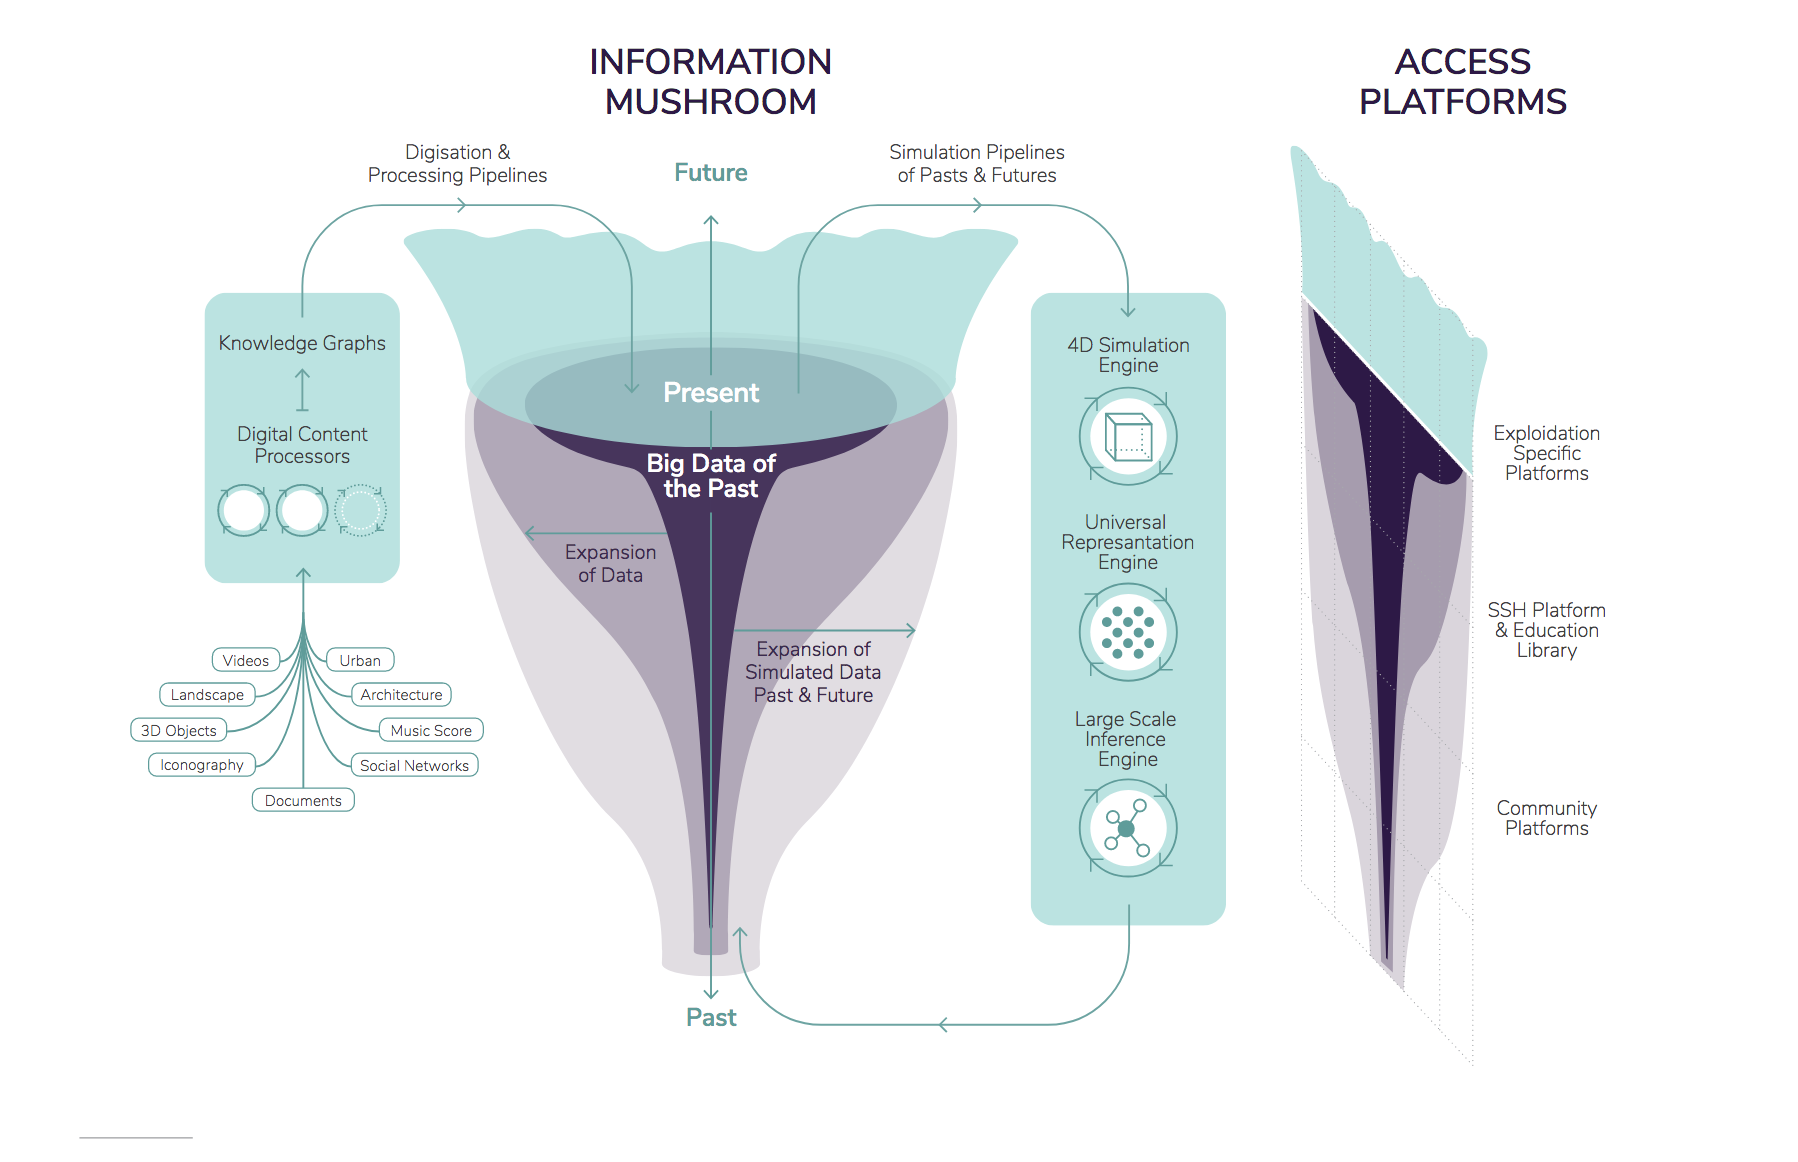
\includegraphics[scale=0.5]{simulation.jpg}
\caption{Représentation schématique des processeurs de contenus et des moteurs d'inférence \textit{© Copyright 2019 Time Machine}}
\end{figure}
\newpage
\item \textbf{Le facteur temps}

En ajoutant la temporalité aux outils de découverte traditionnellement déployés par les \gls{glam}s, Time Machine enrichira l'expérience utilisateur. Son moteur de recherche diachronique ouvrant de nouvelles perspectives de recherches et de valorisation des collections.

\item \textbf{3D et photogrammétrie}

Le \gls{dhlab} s'est spécialisé ces dernières années dans la reconstruction 3D du patrimoine. La \gls{photo} sera au centre des activités de la future initiative qui ne résume pas l'acte de numérisation du patrimoine aux objets 2D, mais promet de mettre l'accent sur la numérisation du patrimoine bâti et des collections muséales.

 Au même titre que Time Machine vise à organiser des centres de numérisation à travers l'Europe afin d'harmoniser les coûts et assurer un certain niveau de qualité, la photogrammétrie bénéficiera de son réseau de spécialistes européens.

\item \textbf{Archivage dans l'ADN}

Les données 3D sont très lourdes et l'ampleur du projet est telle, que de nouvelles solutions de stockage doivent être trouvées afin de permettre une préservation et une consultation de qualité. 

Le projet travaille avec différents partenaires actifs dans cette thématique, dont les propositions futuristes influenceront probablement notre monde de données de demain. L'archivage de données dans l'ADN fait partie de ces technologies prometteuses, permettant de stocker de manière stable et durable des informations, tout en minimisant l'impact écologique alloué à leur préservation. 

\item \textbf{Outils de numérisation}

La marché de la numérisation est encore dans une phase de construction, de nouvelles technologies seront amenées à améliorer les performances obtenues et à s'adapter à la fragilité de certaines typologies de documents. La tomographie\footcite{arte_tomography_nodate} constitue un outil des plus prometteurs, permettant de numériser un objet sans l'ouvrir et d'y déceler des particularités (liées aux fibres du papier etc.) jusqu'alors non visibles par une numérisation plus traditionnelle. Similaire à une radiographie, l'outil est sensible au taux de fer présent dans l'encre des manuscrits et permet d'obtenir des images en coupe de l'intégralité d'un volume. Time Machine promet de contribuer à la recherche sur ces nouveaux outils, et à leurs déploiements. 

\end{enumerate}

%====== RISQUES ET OPPORTUNITES POUR LE PROJET TIME MACHINE

\chapter{Risques et opportunités}

Au-delà des réponses aux enjeux de la numérisation, Time Machine doit faire face à certains risques et opportunités qui découlent de son contexte de création, mais sont aussi induits par les évolutions technologiques et les nouveaux services que le projet se propose de déployer.

\section {Plateforme, usages et accessibilité}

La masse des documents numérisés permet à la fois des recherches orientées, mais offre aussi de nouvelles méthodes de découvertes \inquote{\textit{[...]across genres and disciplines, as well as across institutional and national borders}.\footcite[p.123]{thylstrup_politics_2018}}. 

Au-delà de l'objectif de création de ce corpus de données, se pose la question de son accessibilité. Comment s'assurer que le travail mis en place par Time Machine puisse convenir aux usages des futurs utilisateurs ? Les nouvelles générations semblent peu enclines à la lecture, mais sont entraînées à la communication interactive\footcite{dufrene_numerisation_2013}, seront-elles dès lors à même de s'approprier le contenu et les interfaces de Time Machine ? Comment ne pas se retrouver dépassé par cette masse de données, pour mieux les présenter et les trier ?\footcite{xie_discover_2016}. Avec la numérisation de masse, la capacité humaine de \gls{cur} de ces collections numériques croissantes, semble dépassée. Les capacités cognitives des citoyens ordinaires et la puissance informatique sont de plus en plus sollicitées pour trouver du sens à cette accumulation de données\footcite{thylstrup_politics_2018}. Les fournisseurs de contenu ne peuvent plus se permettre de choisir un outil parmi d'autres, mais se doivent de construire avec tous les standards existants (\gls{api}, \gls{oai}, \gls{rdf} etc.)  pour s'assurer de délivrer leurs données aux plus larges audiences\footcite{dunning_digitising_2009}.

Le projet, à l'instar des précédentes initiatives, propose de réfléchir à de nouvelles formes d'outils de découvertes, promettant de nouvelles expériences aux utilisateurs. \inquote{\textit{An important question for builders of mass digitization projects has therefore been how to build visual and semantic infrastructure that offer the user a sense of meaningful direction as well as a desire to keep browsing.}\footcite[p.110]{thylstrup_politics_2018}}

\subsection{Franchir les barrières territoriales}

S'adressant à une communauté européenne, Time Machine doit être capable de gérer plusieurs langues. Ses utilisateurs souhaiteront pouvoir filtrer les résultats en fonction du langage et effectuer des recherches dans leurs propres idiomes\footcite{xie_discover_2016}. Le déploiement de solutions techniques devra tenir compte des particularités culturelles propres à chaque région et permettre une méthode de partage des données qui traduise automatiquement une requête dans toutes les langues et adresse des résultats provenant de chaque communauté linguistique\footcite{diekema_multilinguality_2012}.

La future plateforme du projet devra veiller à ne pas cloisonner ces résultats par le déploiement de normes occidentales qui préviendraient l'usage des produits à l'extérieur de sa propre communauté\footcite{jones_public_2017}.

\subsection{Être mobile}

La majeure partie du trafic d'Europeana étant générée par des mobiles, et étant donné l'évolution des pratiques et usages, le projet devra développer au plus tôt une telle interface\footcite{xie_discover_2016}\footnote{L'interface mobile de \textit{Diamond} est en cours de développement.}.

\subsection{Favoriser la cocréation}

Pour s'assurer de l'adéquation de la plateforme avec les pratiques des différentes communautés et garantir que ce projet, tourné vers différents publics, ne vienne pas à fonctionner comme la vitrine d'un projet de recherche mené par une communauté professionnelle\footcite{moatti_bibliotheque_2012}, Time Machine se doit de questionner les méthodes de développement traditionnelles et impliquer les usagers dès le début du projet, afin de proposer des services à même de satisfaire leurs besoins interactionnels \footcite[p.7]{dunning_digitising_2009}.

De nombreuses études (instaurées dès la fin des années 1990), ont cherché à comprendre pourquoi les ressources mises en place dans le contexte des humanités numériques n'étaient que peu utilisées par les chercheurs. Ces dernières ont conclu que leurs pratiques ne correspondaient que peu aux recherches empiriques, qui s'intègrent difficilement dans leurs routines de travail. De plus, les usagers semblent se désintéresser rapidement des outils numériques s'ils ne parviennent pas à accéder dès le départ à une information pertinente.\footcite{warwick_digital_2012}\footcite{warwick_studying_2012}. 

Les outils mis en place alors ne s'intéressaient pas du tout aux besoins et usages de leurs utilisateurs, qui étaient considérés comme incapables de comprendre les enjeux du numérique et dès lors de proposer leurs avis

Pour pallier à ce manque d'intérêt et d'adoption des données numériques par les chercheurs en humanités, il faut penser la création des plateformes dans la continuité des pratiques des communautés (ce qui signifie les étudier au préalable et les impliquer dans le processus de création) tout en offrant de nouveaux avantages. \inquote{\textit{If digital resources fit well with what they [users] want to do with them, users will adopt them.\footcite[p.18]{warwick_studying_2012}}}. \inquote{La plateforme fournit une infrastructure ouverte et participative pour des interactions créatrices de valeurs entre des producteurs et des consommateurs externes, dans le cadre des conditions de gouvernance définies par celles-ci.\footcite[p.100]{battu_histoire_2018}}

Les pratiques ne vont pas évoluer d'un coup, il faudra du temps pour que les communautés scientifiques adoptent véritablement ces nouveaux outils. Elles tendent toutefois à évoluer, poussant par exemple les historiens à s'adapter aux nouvelles méthodes d'analyse mises à leur disposition et à développer leurs outils de travail, les faisant prendre conscience de la nécessité de s'impliquer dans les processus de création de ces nouvelles ressources informationnelles. \inquote{If historians do not develop their tools themselves and embrace the goals of digital humanities, they are in danger of having method forced on them that are not compatible with their practice\footcite[p.25]{clavert_histoire_2013}.}

Les données doivent être mises à jour régulièrement, si les utilisateurs ont le sentiment que ces dernières sont dépassées ou datées, ils auront encore plus de difficultés à se les approprier. Leur préservation sur le long-terme doit aussi être garantie, car la recherche scientifique implique de pouvoir réutiliser des jeux de données pour comparer les résultats obtenus. La révolution numérique a instauré le doute concernant la durabilité et la reproductibilité de ces ressources\footcite{clavert_histoire_2013}. Si ces critères de mise à jour et de préservation ne sont pas respectés, il ne sert probablement à rien d'investir dans la création du projet. \inquote{\textit{This is a waste of the (probably) very large amount of money that was spent on its creation. Institutions have only recently begun to develop strategies to deal with this problem.\footcite[p.14]{warwick_studying_2012}}} La pauvreté des informations constitue également une menace, si les jeux de données sont construits uniquement pour un contexte précis, ils ne sauront être utilisés pour d'autres usages. Il faut garantir leur accessibilité intellectuelle afin de prévenir toute mauvaise compréhension des informations\footcite[p.67]{clavert_histoire_2013}.

Au-delà du public scientifique, les voix des communautés et des individus issues du \inquote{grand public} peinent également à être entendues au sein des projets de numérisation de masse \footcite{thelle_persuasive_2011}. La plateforme visant à s'adresser à la plus vaste audience possible, les publics empêchés doivent également être invités à participer au développement des futures interfaces.

Certains auteurs appellent à la construction d'une cyberinfrastructure au service de l'histoire, qui sera coconstruite avec les chercheurs en humanités et s'appuiera sur l'héritage des précédentes initiatives de numérisation, afin d'éviter que le savoir universel demeure détenu, de façon monopolistique, par quelques compagnies privées et puisse bénéficier à tous. Cette cyberinfrastructure devra permettre la création de nouveaux standards capables d'inviter les utilisateurs à chercher de l'information et à la transformer en connaissance\footcite{clavert_histoire_2013}. 

Il semble que Time Machine soit dès lors bien placé pour répondre à ce souhait, pour autant qu'il soit capable d'intégrer ses différents publics-cibles dans ses processus de création et d'inviter le grand-public à se positionner aux côtés de la communauté scientifique.


\subsection{Moteur de recherche ou plateforme de découverte ?}

Time Machine doit se positionner face aux géants de l'information déjà existants, qui ne travaillent pas uniquement à la création de corpus mais à l'indexation du web dans son ensemble. Entre site internet et moteur de recherche, le débat est encore vif et n'apporte que peu de réponse. Certains argumentent qu'un site ne saura rivaliser avec un moteur capable d'en indexer des millions\footcite{moatti_bibliotheque_2012} lorsque d'autres s'interrogent sur la valeur en terme de diffusion, de fonds numérisés ou de moteurs de recherche\footcite{dufrene_numerisation_2013}. Il semble qu'à ce jour, la seule méthode consiste en une forme de collaboration avec ces autres géants, et au déploiement de méthodologie de référencement\footnote{Terme rassemblant toutes les actions visant à améliorer la visibilité d'un site web dans les résultats naturels d'un moteur de recherche. Ces actions impliquent notamment le déploiement de schéma de métadonnées spécifiques, l'usage de mots-clés etc.}, que nous n'aborderons pas plus en détails dans ce présent mémoire.

\section {Crowdsourcing et sciences citoyennes}

Avec l'avènement du web social, de nouveaux moyens de création de ressources informationnelles ont vu le jour, sous la forme du \textit{crowdsourcing} d'abord, reflétant le transfert de processus de travail vers une main d'\oe{}uvre composée d'internautes, puis évoluant vers l'approche plus participative des \gls{cs}. Les entreprises de numérisation de masse et les \gls{glam}s, utilisent traditionnellement les compétences de ces communautés ou individus pour transcrire, corriger ou indexer une sélection de matériel\footcite{coutts_stepping_2017}. 

Le \textit{crowdsourcing} n'est toutefois pas apparu avec l'avénement du numérique, puisque déjà en 1859 la \textit{Philological Society} s'adressait aux citoyens afin de créer ce qui deviendra la première version du \textit{Oxford English Dictionary}\footcite{gupta_enriching_2017}.

De nombreux projets ont recours au \textit{crowdsourcing} pour la création des collections à numériser, invitant les individus à déposer leurs archives personnelles. Cette pratique tend à augmenter l'intérêt et la visibilité de ces initiatives, bien que suscitant des débats sur la qualité et la pertinence de ces nouveaux contenus\footcite{coutts_stepping_2017}. Ces communautés sont également appelées à collaborer dans le déroulement des activités de \gls{photo} liées à la numérisation 3D, qui offrent de nouvelles opportunités à forte valeur ajoutée \inquote{\textit{[...]which has particular intrinsic and instrumental value for themselves, and for their museums in their communities.\footcite[p.22]{chng_crowdsourcing_2019}}}, dans un contexte où les institutions n'ont souvent pas les moyens pour engager des équipes professionnelles \footcite{chng_crowdsourcing_2019}. Certains auteurs appellent à travailler avec les communautés d'expertise déjà existantes afin d'alléger les coûts engendrés par les recherches des détendeurs de droit des \oe{}uvres orphelines, favorisant leur numérisation et garantissant ainsi une marge d'erreur moins grande dans les résultats, puisque ces pratiques intègrent souvent des processus d'auto-vérification\footcite{stobo_i_2018}.

Si le \textit{crowdsourcing} peut prendre une grande variété de formes, en fonction des organisations et du contexte des projets, certains facteurs favorisent leur réussite : accessibilité des plateformes, coût, environnement de travail, ressources humaines etc.\footcite[p.27]{gupta_enriching_2017}. Les projets ayant recours au \textit{crowdsourcing} doivent être pensés dans la durée, puisqu'il est contreproductif de créer une communauté puis de la laisser tomber\footcite[p.15]{warwick_studying_2012}.

S'il faudra encore attendre quelques années pour bien comprendre l'articulation de ces \gls{cs} au sein des projets de numérisation, il est indiscutable qu'elles auront un rôle à jouer. Le modèle économique de Google semble basé sur une certaine idée du \textit{crowdsourcing} faisant appel à l'inventivité et l'intelligence collective du plus grand nombre, \inquote{[...]ces plateformes gratuites rebattent largement les cartes des règles commerciales et des frontières entre le marchand, le public, le commun et leurs différents domaines.\footcite[p.37]{dufrene_numerisation_2013}}. Certains y voient aussi le dernier rempart pour garantir l'accessibilité de toute la connaissance humaine et échapper aux logiques sélectives, dictées par le plébiscite des audiences légitimant certains contenus\footcite[p.107]{mattelart_histoire_2018} : 

\begin{quotation}
Seules des \inquote{sciences citoyennes} qui échappent à l'élitisme tout en se gardant de faire le jeu du populisme peuvent faire contrepoids au projet de société globale de l'information porté par les géants du numérique, leur culture du résultat et du retour sur investissement à court terme. C'est là une condition nécessaire à l'essor de nouveaux usages démocratiques du potentiel du réseau des réseaux.\footcite[p.110]{mattelart_histoire_2018}
\end{quotation}

Time Machine a déjà pris en compte ces communautés dans la création de la feuille de route, il s'agira pour le projet de définir quelle forme et quel rôle attribuer à ces \gls{cs}, garantissant à la fois la préservation d'une continuité démocratique, et porteuses de changement.

\section {Pour un savoir cohérent, égalitaire et éthique}

Au-delà des critères de sélection hérités des politiques documentaires des institutions, Time Machine a l'opportunité de contribuer à créer une connaissance humaine plus juste et égalitaire, qui ne reproduit pas forcément les inégalités hiérarchiques héritées de notre société humaine. Ce défi n'est pas des moindres, puisque jusqu'à présent les plateformes informationnelles ont au contraire servi à renforcer ces mécanismes.

\begin{quotation}
[\textit{Traduction}]
Ce que nous avons constaté dans la pratique, c'est que les plateformes numériques ont la capacité de produire davantage d'homogénéité plutôt que l'inverse, à reproduire les logiques hiérarchiques, inégalités et biais qui structuraient l'existence humaine dans la société avant l'avènement d'internet\footnote{\inquote{\textit{What we have seen in practice is that online platforms have the capacity to produce more homogeneity rather than less, to cultivate and reproduce the hierarchical logics, inequalities, and biases that structured human existence in the world before the internet.}} \cite[p.22]{kim_race_nodate}}.
\end{quotation}

Le monde occidental étant très représenté au sein des acteurs de la numérisation de masse, Time Machine devra porter une attention particulière à la création de liens entre des réseaux de normes et de traditions culturelles différents de son propre milieu, afin de permettre une représentation plus objective de la connaissance qui, elle, s'affranchit aisément des frontières (ce biais impacte également le déploiement d'outils spécifiques à la numérisation, et le développement des plateformes d'accès)\footcite{weiss_examining_2016}\footcite{jones_public_2017}. 

En tant que futur \gls{agr} des collections d'institutions diverses, Time Machine devra veiller à proposer des collections satisfaisantes pour les besoins d'une immense variété de publics. Trouver un équilibre entre la construction de la cohérence et l'exhaustivité à laquelle tend le projet sera l'un des défis de sa future politique documentaire.

De nombreuses questions éthiques sont également soulevées par les initiatives visant à numériser la connaissance universelle. Que doivent-elles faire concernant les objets aux contenus racistes, sexistes, appelant à la haine ou à la suprématie de certains peuples ?\footcite{weiss_examining_2016} Comment garantir que le projet est fidèle aux critères moraux européens ? Si Time Machine veut réussir là où les précédentes initiatives ont échoué, il s'agira d'apporter des réponses à ces questions incontournables et d'offrir davantage qu'une restriction d'accès, comme solution au caractère sensible de certaines données.
\newpage
\section {Résumé des risques et opportunités pour Time Machine}
\begin{table}[H]
\centering
\begin{tabular}{|l|l|}
\hline
\rowcolor[HTML]{2E1A46} 
{\color[HTML]{FFFFFF} \textbf{\begin{tabular}[c]{@{}l@{}}Risques et opportunités\\ pour Time Machine\end{tabular}}}         & {\color[HTML]{FFFFFF} \textbf{Résumé}}                                                                                                                                                                                                                                                                                                                                                                                                                                                                                                                                                                                                                                       \\ \hline
{\color[HTML]{2E1A46} \textbf{\begin{tabular}[c]{@{}l@{}}Plateforme, usages\\ et accessibilité\end{tabular}}}               & \begin{tabular}[c]{@{}l@{}}S'affranchir des barrières territoriales : multilinguisme\\ et prévention contre l'usage de pratiques "occidentales".\\ Être mobile.\\ Favoriser la cocréation : impliquer les futurs usagers dans le\\ développement d'une plateforme ouverte et participative, \\ favorisant des interactions créatrices de valeurs. Veiller aux\\ mises à jour et à l'accessibilité sur le long-terme. Intégrer\\ l'héritage des précédentes initiatives.\\ Moteur de recherche ou plateforme de découverte ? Trouver \\ un positionnement adéquat et déployer des techniques de \\ référencement.\end{tabular}                                                     \\ \hline
{\color[HTML]{2E1A46} \textbf{\begin{tabular}[c]{@{}l@{}}Crowdsourcing et\\ sciences \\ citoyennes\end{tabular}}}           & \begin{tabular}[c]{@{}l@{}}Utiliser les compétences des communautés pour transcrire,\\ corriger ou indexer les collections, sélectionner les documents, \\ participer à la numérisation 3D (photogrammétrie), rechercher \\ les détendeurs des droits d'\oe{}uvres orphelines.\\ Garantir sa réussite, par le développement de plateformes\\ accessibles, une prise en charge des coûts sur le long-terme, un \\ environnement de travail valorisant, des ressources humaines\\ dédiées.\\ Définir le rôle du volontaire entre gardien de la démocratie et de \\ l'accessibilité et briseur des frontières entre marchand, public et\\ commun.\end{tabular} \\ \hline
{\color[HTML]{2E1A46} \textbf{\begin{tabular}[c]{@{}l@{}}Pour un savoir \\ cohérent, égalitaire et\\ éthique\end{tabular}}} & \begin{tabular}[c]{@{}l@{}}Ne pas reproduire les inégalités hiérarchiques de notre société.\\ Créer des passerelles au-delà du monde occidental pour \\ permettre une représentation nouvelle du savoir.\\ Trouver un équilibre entre construction de la cohérence et quête\\ d'exhaustivité.\\ Adresser les questions éthiques posées par la création des \\ collections et les objectifs du projet.\end{tabular}                                                                                                                                                                                                                                                             \\ \hline
\end{tabular}
\caption {Résumé des risques et opportunités pour Time Machine}
\end{table}

%====== POURQUOI NUMERISER EN MASSE

\chapter{\textit{Pourquoi} numériser en masse ? }

Nous avons essayé à travers ce mémoire, de montrer la complexité des entreprises de numérisation de masse. Du passage à l'échelle des premières entreprises de numérisation jusqu'à l'avènement des \gls{bigd}, ces projets ont franchi les portes de leurs institutions pour se mêler à l'agenda politique et prendre une part active dans la définition des standards du web. Porteurs de nombreux intérêts mélangeant biens communs et usages commerciaux, ils semblent rassembler sous la même bannière, des idées à priori opposées et des acteurs issus du monde public et du monde privé. Leurs poids financiers et les débats légaux qu'ils suscitent les poussent à inventer de nouvelles formes de partenariats et confrontent la sphère politique aux usages du numérique. Time Machine, bien que né dans un centre de recherche en humanités digitales, fédère au-delà de son milieu académique, s'affranchissant des barrières nationales, et à travers ses ambitions de recherche et de valorisation, semble incarner les questionnements de tous sur notre société numérique. Le projet, comme ses précurseurs, ne se laisse pas résumer par une seule question. Dernière initiative de la lignée des projets de numérisation de masse, Time Machine entend préserver le passé tout en modifiant l'avenir.

Au-delà des aspects techniques et opérationnels liés à l'envergure de ces projets, il semble urgent de considérer les questions du \textit{pourquoi}, afin de mieux comprendre l'impact d'initiatives de telle ampleur sur l'organisation de notre société et les industries qui la composent. Les questions soulevées sont nombreuses et nous ne prétendrons pas pouvoir leur apporter à toutes un début de réflexion, nous avons préféré introduire ce débat à travers deux questions qui nous semblent peu abordées par la communauté scientifique dans le cadre de tels projets\footnote{Le temps que nous avons eu à disposition pour la rédaction du mémoire étant cependant limité, il est probable que de nombreuses publications n'aient pas été prises en compte dans notre revue de la littérature. Notre impression est dès lors subjective.} : la surveillance de masse et le positionnement de ces initiatives par rapport aux acteurs culturels et patrimoniaux plus traditionnels.

\section {Influence de masse}

Bien que les projets de numérisation de masse se construisent autour de l'objectif de rendre accessible le savoir en ligne, et que les complexités liées à la construction des infrastructures et les questions financières, politiques, éthiques et légales qui en découlent tendent à accaparer toute l'attention, une autre forme de connaissance est acquise de manière plus discrète. Elle est sans doute motivée par des intérêts divergents en fonction des acteurs de chaque initiative et justifiée par le souci de proposer une meilleure expérience aux utilisateurs ou obtenir de nouvelles formes de financement. Nos actes et pensées d'usagers sont néanmoins précieusement récoltés, nous livrant à la merci de nouvelles logiques économiques et régimes politiques : \inquote{\textit{[...]as we collect and connect, we are also ourselves collected and connected.}\footcite[p.138]{thylstrup_politics_2018}}. 
Si les défenseurs de l'innovation argumentent qu'il ne sert à rien de s'effrayer de l'impact de ces collectes de données, qui auraient moins d'effet que les spots publicitaires traditionnels accompagnant les campagnes politiques : \inquote{\textit{We freak out over the unsavory influence of social media on our politics, while TV's partisan influence on elections is far, far greater than Facebook's.}\footcite{kelly_ar_2019}}. Il semble important de nous rappeler que nous avons un rôle à jouer dans la définition éthique des projets de cette envergure.

Les projets de numérisation de masse ont de plus recours aux technologies dites persuasives pour développer l'interface de leurs plateformes\footnote{Les technologies persuasives sont conçues pour modifier les pratiques et comportements des usagers à travers la persuasion et l'influence sociale, sans utiliser la force. Elles s'incarnent souvent dans le graphisme des interfaces et sont motivées par la recherche du \inquote{moindre effort}. Par exemple un usager ayant appris à effectuer des recherches sur Google, sera d'autant plus enclin à utiliser la même méthode pour accéder aux ouvrages de \textit{Google Books}. \cite{thelle_persuasive_2011}}, ces technologies basées sur les principes du \inquote{moindre effort} contribuent à la mise en place de mécanismes de pouvoir invisibles, susceptibles d'influencer notre liberté d'opinion et la démocratie\footcite{thelle_persuasive_2011}. 

Le pouvoir de ces entreprises étant souvent le résultat d'un petit nombre de personnes qui décident pour toutes les autres\footcite{thylstrup_politics_2018}, ce sont néanmoins les utilisateurs finaux qui permettent à ce marché d'exister. Dès lors une prise de conscience de ces enjeux permettrait de rétablir un équilibre entre tous ces intérêts divergents, et contribuerait à garantir que l'emploi de ces technologies se fasse bien au service de la démocratie.


\section {Vers la création d'un nouvel acteur de l'information}

Nous nous sommes interrogée, en introduction de ce mémoire, sur la place occupée par ces projets au sein de la famille des institutions culturelles ayant pour mission de rendre la connaissance accessible à tous (\gls{glam}), puisque les initiatives de numérisation de masse sont d'abord et premièrement motivées par une mission similaire : celle de restituer au monde la connaissance, en s'assurant de son accessibilité dans notre société numérique, à travers la numérisation.

L'étude des différents enjeux de la numérisation et l'analyse d'autres initiatives témoignent que le succès de ces projets n'est pas seulement corrélé aux seules capacités des institutions culturelles et patrimoniales, mais implique un mélange d'acteurs issus du monde privé et du monde public répondant à des communautés de pratiques et à des politiques diverses, s'organisant au sein d'un réseau. L'infrastructure commune aux membres de ce réseau doit être par essence souple et flexible, capable de s'adapter à la diversité de ses partenaires, tout en définissant un certain nombre de standards et de routines permettant une convergence des pratiques. La mise en place de ces standards aboutit à des formes de politiques internes au réseau et contribuent à renforcer son pouvoir vis-à-vis des politiques extérieures. Le pouvoir du réseau se construisant souvent en même temps que le réseau lui-même : \inquote{\textit{through standardization, inventions become commonplace, novelties become mundane, and the local becomes universal.}\footcite[p.31]{thylstrup_politics_2018}}.

Le déploiement d'activités de numérisation de masse offre la perspective de création de nouvelles sources de revenus, attirant industries et entreprises privées au sein de leurs réseaux. Les entreprises culturelles étant depuis toujours empreintes de capitalisme, la numérisation de masse a de facto introduit une nouvelle forme de capitalisme imposée à notre mémoire culturelle : le capitalisme numérique\footcite{thylstrup_politics_2018}. 

Ces initiatives semblent, de plus, contribuer à inscrire les institutions patrimoniales et leurs usagers au sein d'une nouvelle constellation de pouvoir et de politiques : \inquote{\textit{[...] these infrapolitical imaginaries in fact show the complexity of mass digitization projects in their reinscription of users and cultural memory institutions in new constellations of power and politics.} \footcite[p.131]{thylstrup_politics_2018}}.

Plus que de simples plateformes de valorisation visant à rendre les données du passé accessibles, le déploiement de l'infrastructure des projets de numérisation de masse soulève de grandes questions concernant l'éthique, les politiques, le pouvoir et la protection des individus au sein de la sphère numérique. Issues de différents courants politiques, ces initiatives viennent bouleverser l'organisation existante du pouvoir.
\begin{quotation}
[\textit{Traduction}]
La luxuriante dimension des initiatives de numérisation de masse semble émerger des décombres de processus politiques perturbateurs et tumultueux, qui viennent violemment disloquer les frontières établies et les dynamiques de pouvoir, donnant naissance à de nouvelles formes qui doivent encore être interprétées. \footnote{\inquote{\textit{Rather, the productive dimensions of mass digitization emerge from the rubble of disruptive and turbulent political processes that violently dislocate established frontiers and power dynamics and give rise to new ones that are yet to be interpreted.\cite[p.137]{thylstrup_politics_2018}}}} 
\end{quotation}

Difficile en conséquent de considérer ces initiatives comme une simple évolution des activités conduites par les institutions culturelles et patrimoniales. Si ces projets tendent à bouleverser les règles établies et sont suffisamment puissants pour impacter les politiques et proposer une nouvelle forme d'économie, ils se doivent probablement d'être considérés en tant que nouvelle entité (ou acteur de l'information), dont les particularités et caractéristiques doivent encore être pleinement étudiées et comprises, afin de ne pas laisser ce pouvoir émergent se construire en-dehors des règles fondatrices de notre société.



\part*{Conclusion}
\addcontentsline{toc}{part}{Conclusion}
\markboth{Conclusion}{Conclusion} 

Étudier la numérisation de masse, tout en participant à la construction d'une telle initiative a permis de nourrir un intéressant dialogue entre problématiques du terrain et théorie. Les enjeux de la numérisation de masse se dessinant au fil de notre état de l'art et de la création de la feuille de route, l'apport pratique a contribué à élargir le champ initial de la recherche, et la recherche a pu influencer la réalité des propositions. La réalisation de notre mission de stagiaire au sein du projet Time Machine, notre collaboration à l'élaboration des propositions de la feuille de route et la rédaction du présent mémoire, nous ont demandé un important travail de réflexion sur trois axes : la définition des projets de numérisation (contexte, histoire, caractéristiques et enjeux), l'analyse de précédentes initiatives (motivations et réponses apportées aux enjeux identifiés), l'étude du projet Time Machine (réponses apportées aux enjeux, innovations, risques et opportunités, potentiel impact). Nous proposons d'esquisser un bilan des propositions contenues dans ces trois parties de notre mémoire ainsi que des enseignements tirés de notre expérience de stagiaire.

La première partie, entièrement théorique, nous a permis d'abord de retracer l'origine des premières initiatives de numérisation, mêlant développements technologiques et élargissement des activités des institutions culturelles et patrimoniales. Les développements numériques tendant à s'accélérer, les années 1990 voient apparaître les précurseurs des projets de numérisation de masse et les années 2000 marquent la naissance des premières recommandations et directives européennes, appelées à favoriser la croissance de l'économie numérique et à contribuer à l'orientation de ces initiatives d'envergure, la photogrammétrie figurant désormais en bonne place dans les objectifs de numérisation européens. Time Machine s'inscrit ainsi dans la continuité des premiers projets de bibliothèque universelle qui se voyaient également limités par des développements technologiques, dont la taille nécessitait un besoin de standardisation et ne manquaient pas de voir des décisions politiques ou historiques influencer la création de leurs collections. L'histoire nous montre que l'avènement du numérique a très vite impliqué une grande mixité parmi les acteurs des projets, qui se sont confrontés aux questions du droit d'auteur et ont \oe{}uvré au déploiement de solutions politiques.

Dans un deuxième temps, nous nous sommes attelée au \textit{comment} des initiatives de numérisation de masse, à la définition de leurs caractéristiques et aux enjeux reliés. Par nature complexes, ces initiatives ne se laissent pas facilement résumer et semblent gagner en difficultés à mesure que l'on cherche à les comprendre. Nous nous sommes basée sur notre analyse historique et expérience de stagiaire afin de proposer une sélection de cinq enjeux à étudier plus précisément (la collaboration, le financement public-privé, le droit d'auteur, l'interopérabilité, le stockage sur le long-terme). 

Au vu de la taille des projets, appelés à articuler intérêts divers et pratiques multiples, la collaboration apparaît comme un facteur clé de réussite. Une numérisation massive, implique des coûts conséquents dont les institutions publiques ne peuvent, seules, prendre la responsabilité. Des partenariats public-privé semblent inévitables, mais rendent plus difficiles l'inscription de ces projets dans une démarche d'ouverture et de transparence. Les directives actuelles du droit d'auteur ne facilitent pas la circulation des données numériques et préviennent la représentation de celles issues de notre passé le plus récent, Time Machine devra oser la prise de risque s'il ne veut pas être limité par ces barrières. Sortir des \inquote{silos} peut se faire à condition de veiller à une interopérabilité technique et des politiques documentaires à la hauteur des ambitions des projets de numérisation de masse, en arrière-fonds la collaboration semble encore détenir les clés du succès. Appréhender la préservation des données pour en favoriser les usages est essentiel à tout projet de numérisation de masse. Time Machine aura pour tâche de comprendre les nuances propres à chaque enjeu et d'intégrer la matérialité des solutions au sein de son infrastructure. La création de cette infrastructure ne se fera pas sans la mise en place d'un cadre opérationnel à même de réconcilier les pratiques du monde de la documentation, du web et de l'industrie, afin de planifier et exécuter la transformation des données du passé en données numériques.

Notre travail nous permet de conclure que si le projet veut réussir à établir de nouvelles normes et apporter des réponses satisfaisantes à ces différents enjeux, il lui faudra non seulement disposer de grands moyens financiers, mais être capable d'instaurer un dialogue privilégié avec chaque membre de son réseau, tout en composant avec le cadre externe du projet (légal et politique) qui, sans avoir apporté de réponses complètes aux problématiques du droit d'auteur, nourrit de hautes ambitions pour la numérisation du patrimoine européen. Alors que le financement du projet est des plus incertain, Time Machine doit réussir à se positionner comme réseau d'influence, à même d'accroître le soutien politique dont il bénéficie et espérer ainsi briser certaines barrières territoriales et légales qui rendent compliquée la réalisation du \gls{bigd} du passé.

La deuxième partie est consacrée à l'étude des motivations d'autres projets de numérisation de masse (\textit{Google Books}, Europeana, \textit{HathiTrust} et \textit{the Digital Public Library of America}) et aux réponses apportées par ces initiatives aux enjeux de la numérisation. Cette comparaison nous a permis de déduire que les frontières séparant ces projets sont poreuses, chacun se basant sur les réalisations des autres pour construire de nouveaux développements. Les initiatives sont conscientes de cette complémentarité et travaillent ensemble à élaborer de nouvelles solutions aux différents enjeux. Nous concluons cette recherche par le constat que plutôt que de chercher à catégoriser ces initiatives, il semble plus intéressant de les considérer comme un tout, afin de pouvoir déplacer le spectre de la réflexion au niveau de leur ensemble et ne pas seulement s'arrêter sur les détails qui les composent. Time Machine devra lui aussi développer des ponts avec ces grands réseaux, et trouver un équilibre entre le phénomène de mondialisation culturelle qui les accompagne et la préservation des particularités locales et régionales de ses partenaires.

Enfin notre troisième partie, plus concrète, est d'abord pour nous l'occasion de présenter les propositions contenues dans la feuille de route en analysant les réponses apportées aux différents enjeux par Time Machine. Puisque l'agenda, entre les recherches conduites pour le mémoire et les échéances de rendu européennes, n'a pas toujours coïncidé, nous proposons un certain nombre d'amendements. Ils visent à accroître la collaboration avec les \gls{agr}s que sont les Time Machines locales, à mieux prendre en compte les usages du public dans la gestion des droits d'auteur, à favoriser la préservation sur le long-terme par des directives techniques et à compléter les outils destinés à garantir l'interopérabilité afin de sortir de la logique des \inquote{silos}. Nous argumentons ensuite que ce qui distingue Time Machine des autres entreprises de numérisation de masse, est l'intégration de toutes les parties publiques ou privées ou sein d'un même réseau (le projet ne faisant pas la distinction entre collaborateurs internes et futurs exploitants), et le déploiement d'innovations technologiques, pour certaines basées sur l'intelligence artificielle, au service de la création du \gls{bigd} du passé. Fort de ces propositions novatrices, Time Machine accroît sa popularité auprès d'acteurs attirés par les nouvelles perspectives offertes par la démarche inclusive et la crédibilité technologique du projet.

Notre travail d'analyse historique et des enjeux, nous a permis de définir un certain nombre d'éléments constituants des risques ou opportunités. Time Machine devra, au-delà du déploiement d'infrastructures et routines cohérents, proposer une plateforme en accord avec les besoins et attentes des différentes communautés composant son public-cible en évitant les méthodologies limitées au monde occidental, pour ne pas biaiser le développement de ses collections et cloisonner les usages futurs. Favoriser la cocréation devrait permettre à Time Machine de proposer des solutions fédératrices au-delà des frontières territoriales et académiques. Résolument tourné vers le futur, le projet se devra également de refléter les nouvelles pratiques induites par le numérique et proposer au grand public un rôle actif et créateur de valeur, en promouvant les \gls{cs}. Time Machine a l'opportunité de pouvoir donner à l'Europe une plateforme aux contenus égaux et éthiques, ne cherchant pas à refléter l'histoire telle que déjà écrite, mais à en offrir une nouvelle reproduction. 

Nous concluons cette partie sur le constat que si de nombreuses études se consacrent aux enjeux techniques et organisationnels liés aux projets de numérisation de masse, trop peu de chercheurs s'intéressent aux questions du \textit{pourquoi}. Pourtant la portée de ces projets dépasse les frontières du monde culturel et patrimonial et ces réseaux détiennent une forme de pouvoir susceptible d'avoir des répercussions sur notre société. 

Réseau définitivement tourné vers les innovations numériques, Time Machine semble déjà incarner les attentes d'une classe dirigeante européenne inquiète de bénéficier des retombées économiques offertes par ce nouveau monde. S'inscrivant dans le suivi des politiques de mondialisation, et s'adressant à une audience plus large que celle réservée aux institutions culturelles et patrimoniales, le projet ouvre le dialogue au sein des plus hautes sphères du pouvoir européen et suscite avant même le déploiement de son infrastructure, l'intérêt des foules. Ce nouvel acteur des initiatives de numérisation de masse semble déjà détenir une forme de pouvoir. Seules des recherches plus avancées permettront de définir avec assurance si ce dernier est limité aux partenaires de son réseau, où s'étend au-delà et touche la sphère politique. Nous pensons que pour permettre l'étude de ces nouveaux phénomènes et être en adéquation avec leur complexité, il est plus que temps de considérer les acteurs de la numérisations de masse comme de nouvelles entités informationnelles, dont les contours évoluent certes, mais entraînent des répercussions en dehors du milieu des institutions culturelles et patrimoniales, qui viennent ébranler un certain ordre établi.

A l'instar des précédentes initiatives de numérisation de masse, le projet Time Machine semble apporter autant de nouvelles solutions que de questionnements. Si le projet aboutit et réussit une intégration équilibrée de tous ces éléments, il deviendra sans doute un acteur informationnel, politique, économique et culturel de poids. Espérons alors, que la prophétie du \textit{mirrorworld} se trompe lorsqu'elle décrit les futurs services développés comme appelés à devenir des biens payants au même titre que l'eau et l'électricité\footcite{kelly_ar_2019}, et que Time Machine demeurera un outil au service de l'égalité et de la démocratie, libre et gratuit.

%-----------ANNEXES--------------

\appendix
	\part*{Annexes}	
	\addcontentsline{toc}{part}{Annexes}
	\chapter{Prémisses de la numérisation\label{premisse}}
	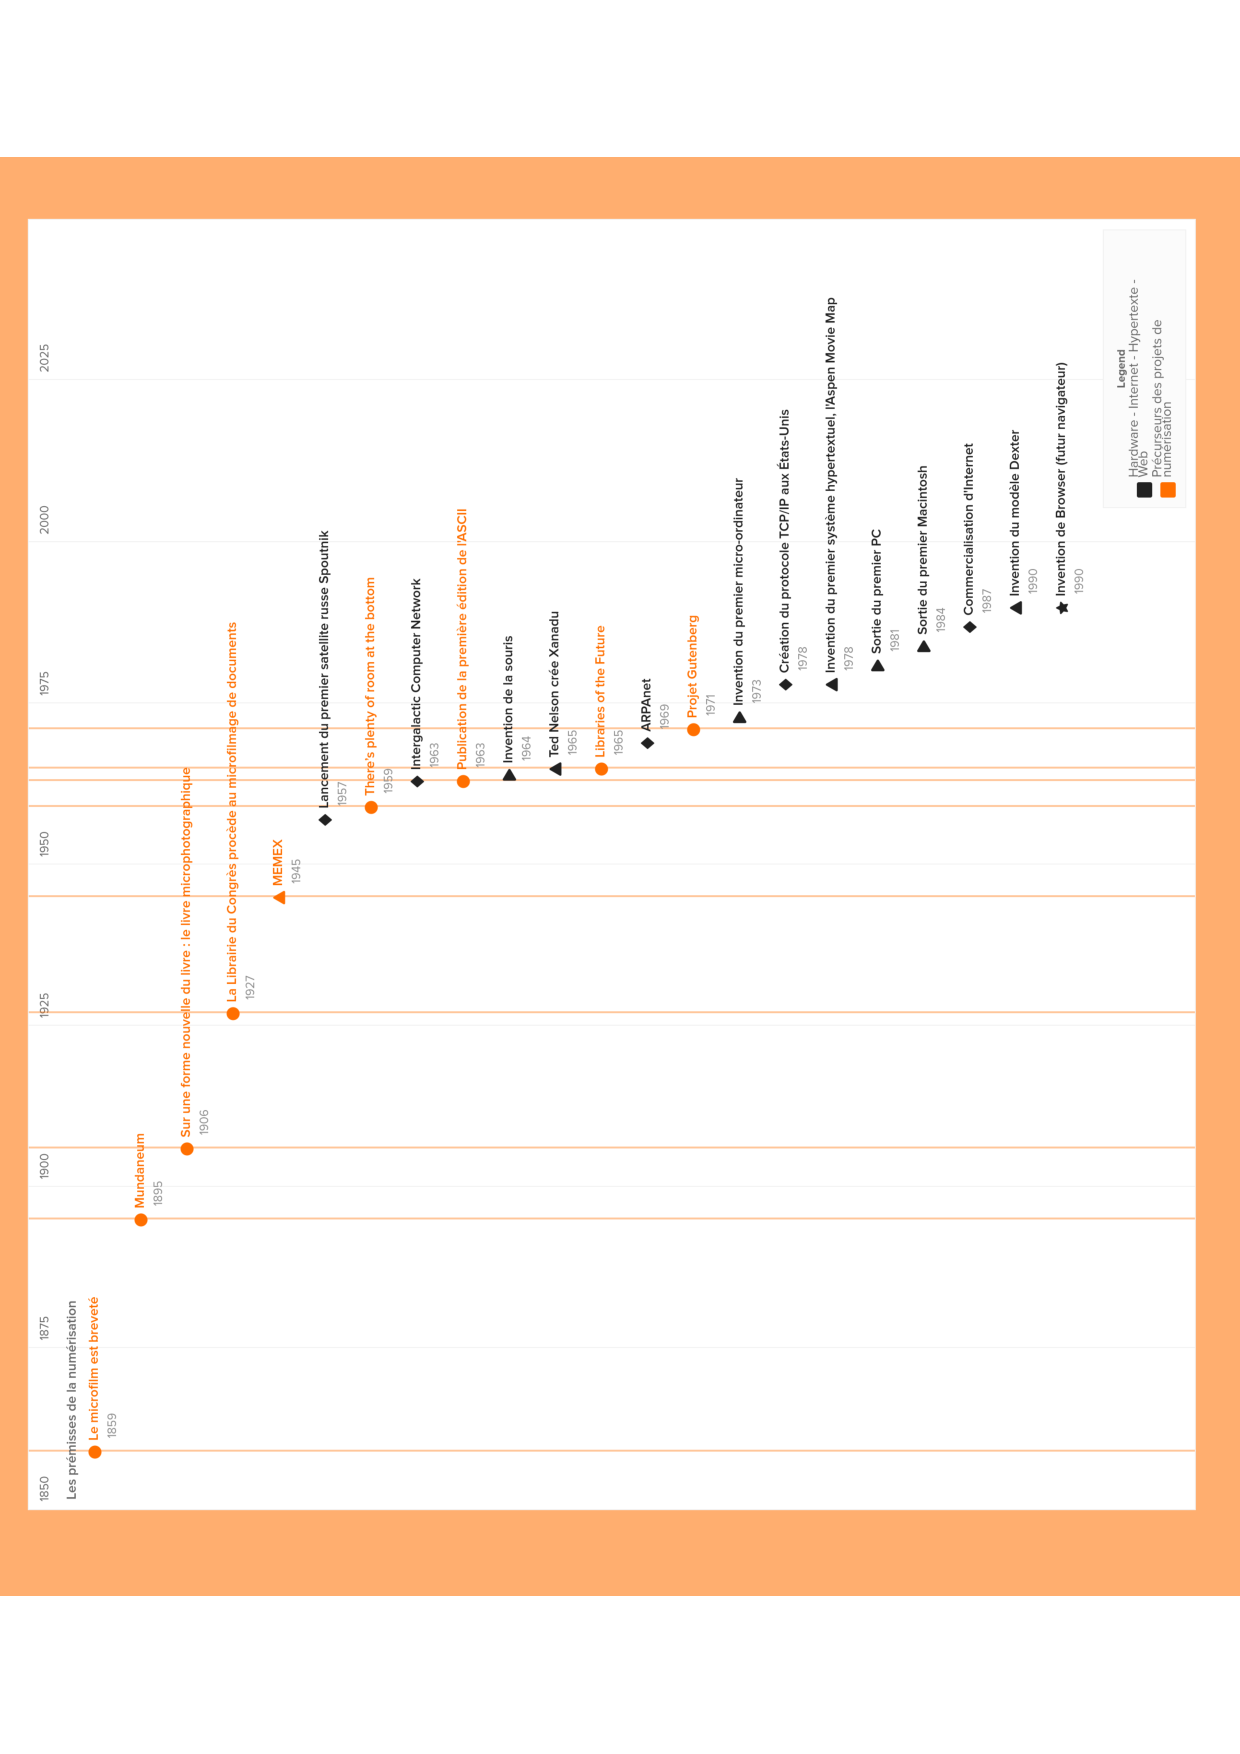
\includepdf[fitpaper,rotateoversize]{annexe/premisse_image.pdf}
	\includepdf[pages=2-3, fitpaper,rotateoversize]{annexe/premisse_texte.pdf}
	\chapter{Factsheet\label{factsheet}}
	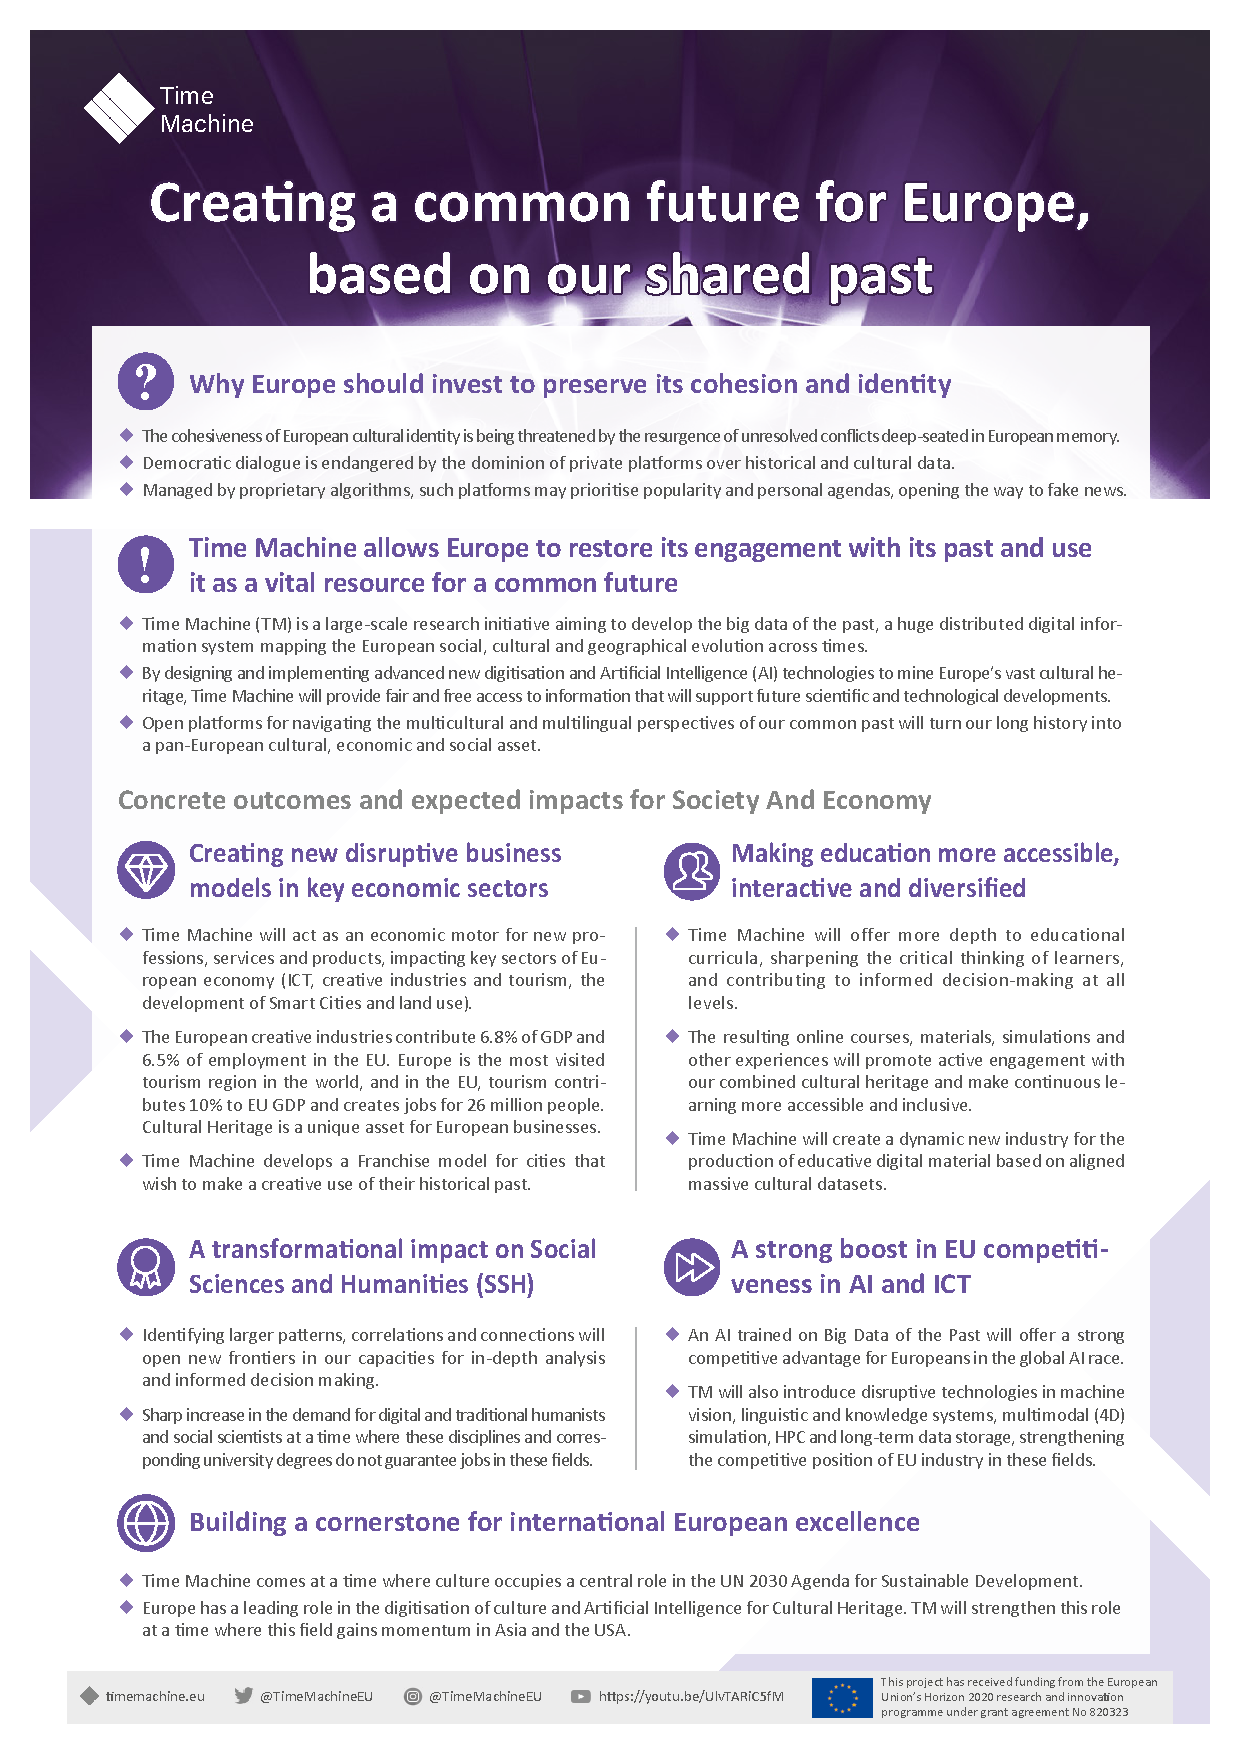
\includepdf[pages={1,2}]{annexe/factsheet.pdf}


\backmatter
%-----------GLOSSAIRE--------------
\printglossary 
%-----------TABLES ET FIGURES--------------
\listoffigures
\listoftables
\tableofcontents
\end{document}






